% Options for packages loaded elsewhere
%DIF LATEXDIFF DIFFERENCE FILE
%DIF DEL C:/Users/timothy.j.miller/Documents/work/SSRTWG/SSRTWG/Project_0/manuscript/manuscript.tex      Fri May  2 15:34:35 2025
%DIF ADD C:/Users/timothy.j.miller/Documents/work/SSRTWG/SSRTWG/Project_0/manuscript/manuscript_R1.tex   Mon Sep 29 11:27:09 2025
\PassOptionsToPackage{unicode}{hyperref}
\PassOptionsToPackage{hyphens}{url}
%DIF 4d4
%DIF < %
%DIF -------
\documentclass[
  12pt,
]{article}
%DIF 8a7-8
\usepackage{xcolor} %DIF > 
\usepackage[margin=1in]{geometry} %DIF > 
%DIF -------
\usepackage{amsmath,amssymb}
%DIF 9c10
%DIF < \usepackage{lmodern}
%DIF -------
\setcounter{secnumdepth}{5} %DIF > 
%DIF -------
\usepackage{iftex}
\ifPDFTeX
  \usepackage[T1]{fontenc}
  \usepackage[utf8]{inputenc}
  \usepackage{textcomp} % provide euro and other symbols
\else % if luatex or xetex
%DIF 16c17
%DIF <   \usepackage{unicode-math}
%DIF -------
  \usepackage{unicode-math} % this also loads fontspec %DIF > 
%DIF -------
  \defaultfontfeatures{Scale=MatchLowercase}
  \defaultfontfeatures[\rmfamily]{Ligatures=TeX,Scale=1}
\fi
%DIF 20a21-24
\usepackage{lmodern} %DIF > 
\ifPDFTeX\else %DIF > 
  % xetex/luatex font selection %DIF > 
\fi %DIF > 
%DIF -------
% Use upquote if available, for straight quotes in verbatim environments
\IfFileExists{upquote.sty}{\usepackage{upquote}}{}
\IfFileExists{microtype.sty}{% use microtype if available
  \usepackage[]{microtype}
  \UseMicrotypeSet[protrusion]{basicmath} % disable protrusion for tt fonts
}{}
\makeatletter
\@ifundefined{KOMAClassName}{% if non-KOMA class
  \IfFileExists{parskip.sty}{%
    \usepackage{parskip}
  }{% else
    \setlength{\parindent}{0pt}
    \setlength{\parskip}{6pt plus 2pt minus 1pt}}
}{% if KOMA class
  \KOMAoptions{parskip=half}}
\makeatother
%DIF 36-45d41
%DIF < \usepackage{xcolor}
%DIF < \IfFileExists{xurl.sty}{\usepackage{xurl}}{} % add URL line breaks if available
%DIF < \IfFileExists{bookmark.sty}{\usepackage{bookmark}}{\usepackage{hyperref}}
%DIF < \hypersetup{
%DIF <   pdftitle={An investigation of factors affecting inferences from and reliability of state-space age-structured assessment models},
%DIF <   pdfauthor={Timothy J. Miller1,2; Greg Britten3; Elizabeth N. Brooks2; Gavin Fay4; Alex Hansell2; Christopher M. Legault2; Chengxue Li2; Brandon Muffley5; Brian C. Stock6; John Wiedenmann7},
%DIF <   hidelinks,
%DIF <   pdfcreator={LaTeX via pandoc}}
%DIF < \urlstyle{same} % disable monospaced font for URLs
%DIF < \usepackage[margin=1in]{geometry}
%DIF -------
\usepackage{graphicx}
\makeatletter
%DIF 48-54c43-52
%DIF < \def\maxwidth{\ifdim\Gin@nat@width>\linewidth\linewidth\else\Gin@nat@width\fi}
%DIF < \def\maxheight{\ifdim\Gin@nat@height>\textheight\textheight\else\Gin@nat@height\fi}
%DIF < \makeatother
%DIF < % Scale images if necessary, so that they will not overflow the page
%DIF < % margins by default, and it is still possible to overwrite the defaults
%DIF < % using explicit options in \includegraphics[width, height, ...]{}
%DIF < \setkeys{Gin}{width=\maxwidth,height=\maxheight,keepaspectratio}
%DIF -------
\newsavebox\pandoc@box %DIF > 
\newcommand*\pandocbounded[1]{% scales image to fit in text height/width %DIF > 
  \sbox\pandoc@box{#1}% %DIF > 
  \Gscale@div\@tempa{\textheight}{\dimexpr\ht\pandoc@box+\dp\pandoc@box\relax}% %DIF > 
  \Gscale@div\@tempb{\linewidth}{\wd\pandoc@box}% %DIF > 
  \ifdim\@tempb\p@<\@tempa\p@\let\@tempa\@tempb\fi% select the smaller of both %DIF > 
  \ifdim\@tempa\p@<\p@\scalebox{\@tempa}{\usebox\pandoc@box}% %DIF > 
  \else\usebox{\pandoc@box}% %DIF > 
  \fi% %DIF > 
} %DIF > 
%DIF -------
% Set default figure placement to htbp
%DIF 56d54
%DIF < \makeatletter
%DIF -------
\def\fps@figure{htbp}
\makeatother
%DIF 59-62c56-66
%DIF < \setlength{\emergencystretch}{3em} % prevent overfull lines
%DIF < \providecommand{\tightlist}{%
%DIF <   \setlength{\itemsep}{0pt}\setlength{\parskip}{0pt}}
%DIF < \setcounter{secnumdepth}{5}
%DIF -------
% definitions for citeproc citations %DIF > 
\NewDocumentCommand\citeproctext{}{} %DIF > 
\NewDocumentCommand\citeproc{mm}{% %DIF > 
  \begingroup\def\citeproctext{#2}\cite{#1}\endgroup} %DIF > 
\makeatletter %DIF > 
 % allow citations to break across lines %DIF > 
 \let\@cite@ofmt\@firstofone %DIF > 
 % avoid brackets around text for \cite: %DIF > 
 \def\@biblabel#1{} %DIF > 
 \def\@cite#1#2{{#1\if@tempswa , #2\fi}} %DIF > 
\makeatother %DIF > 
%DIF -------
\newlength{\cslhangindent}
\setlength{\cslhangindent}{1.5em}
\newlength{\csllabelwidth}
\setlength{\csllabelwidth}{3em}
%DIF 67-71c71-75
%DIF < \newlength{\cslentryspacingunit} % times entry-spacing
%DIF < \setlength{\cslentryspacingunit}{\parskip}
%DIF < \newenvironment{CSLReferences}[2] % #1 hanging-ident, #2 entry spacing
%DIF <  {% don't indent paragraphs
%DIF <   \setlength{\parindent}{0pt}
%DIF -------
\newenvironment{CSLReferences}[2] % #1 hanging-indent, #2 entry-spacing %DIF > 
 {\begin{list}{}{% %DIF > 
  \setlength{\itemindent}{0pt} %DIF > 
  \setlength{\leftmargin}{0pt} %DIF > 
  \setlength{\parsep}{0pt} %DIF > 
%DIF -------
  % turn on hanging indent if param 1 is 1
  \ifodd #1
%DIF 74-75c78-79
%DIF <   \let\oldpar\par
%DIF <   \def\par{\hangindent=\cslhangindent\oldpar}
%DIF -------
   \setlength{\leftmargin}{\cslhangindent} %DIF > 
   \setlength{\itemindent}{-1\cslhangindent} %DIF > 
%DIF -------
  \fi
  % set entry spacing
%DIF 78-80c82-83
%DIF <   \setlength{\parskip}{#2\cslentryspacingunit}
%DIF <  }%
%DIF <  {}
%DIF -------
  \setlength{\itemsep}{#2\baselineskip}}} %DIF > 
 {\end{list}} %DIF > 
%DIF -------
\usepackage{calc}
%DIF 82-84c85-87
%DIF < \newcommand{\CSLBlock}[1]{#1\hfill\break}
%DIF < \newcommand{\CSLLeftMargin}[1]{\parbox[t]{\csllabelwidth}{#1}}
%DIF < \newcommand{\CSLRightInline}[1]{\parbox[t]{\linewidth - \csllabelwidth}{#1}\break}
%DIF -------
\newcommand{\CSLBlock}[1]{\hfill\break\parbox[t]{\linewidth}{\strut\ignorespaces#1\strut}} %DIF > 
\newcommand{\CSLLeftMargin}[1]{\parbox[t]{\csllabelwidth}{\strut#1\strut}} %DIF > 
\newcommand{\CSLRightInline}[1]{\parbox[t]{\linewidth - \csllabelwidth}{\strut#1\strut}} %DIF > 
%DIF -------
\newcommand{\CSLIndent}[1]{\hspace{\cslhangindent}#1}
%DIF 86a89-91
\setlength{\emergencystretch}{3em} % prevent overfull lines %DIF > 
\providecommand{\tightlist}{% %DIF > 
  \setlength{\itemsep}{0pt}\setlength{\parskip}{0pt}} %DIF > 
%DIF -------
\usepackage{url}
\usepackage{setspace}
%\singlespacing
%\onehalfspacing
\doublespacing
\usepackage{lineno}
\linenumbers
\usepackage[belowskip=0pt,aboveskip=0pt]{caption}
\usepackage{relsize}
\usepackage{float}
\usepackage{lscape}
\usepackage{longtable}
\usepackage{amsmath,rotating}
\usepackage[scanall]{psfrag}
\usepackage{bm}
\usepackage{caption,graphics}
\usepackage{graphicx}
\usepackage{sectsty}
\usepackage{color}
\usepackage{fancyhdr}
\usepackage{xspace}
\usepackage{textcomp}
\usepackage{upgreek}
\renewcommand\figurename{Fig.}
\captionsetup{labelsep=period, singlelinecheck=false}
\newcommand{\changesize}[1]{\fontsize{#1pt}{#1pt}\selectfont}
\renewcommand{\arraystretch}{1.5}
%\renewcommand\theadfont{}

\newcommand{\Fmsy}{\ensuremath{F_{\text{MSY}}}\xspace}
\newcommand{\Fspr}[1]{\ensuremath{F_{\text{{#1}\%}}}\xspace}
\newcommand{\afrb}{Alaska Fishery Research Bulletin\xspace}
\newcommand{\ajms}{African Journal of Marine Science\xspace}
\newcommand{\amb}{Advances in Marine Biology\xspace}
\newcommand{\bms}{Bulletin of Marine Science\xspace}
\newcommand{\bjssf}{Bulletin of the Japanese Society of Scientific Fisheries\xspace}
\newcommand{\cb}{Conservation Biology\xspace}
\newcommand{\cjfas}{Canadian Journal of Fisheries and Aquatic Sciences\xspace}
\newcommand{\ea}{Ecological Applications\xspace}
\newcommand{\eer}{Evolutionary Ecology Research\xspace}
\newcommand{\elet}{Ecology Letters\xspace}
\newcommand{\emod}{Ecological Modelling\xspace}
\newcommand{\ebf}{Environmental Biology of Fishes\xspace}
\newcommand{\ff}{Fish and Fisheries\xspace}
\newcommand{\fo}{Fisheries Oceanography\xspace}
\newcommand{\fr}{Fisheries Research\xspace}
\newcommand{\fb}{Fishery Bulletin\xspace}
\newcommand{\ijms}{ICES Journal of Marine Science\xspace}
\newcommand{\iccat}{Collective Volume of Scientific Papers ICCAT\xspace}
\newcommand{\jae}{Journal of Animal Ecology\xspace}
\newcommand{\jai}{Journal of Applied Ichthyology\xspace}
\newcommand{\jdc}{Journal Du Conseil International Pour L'exploration De La Mer\xspace}
\newcommand{\jdcp}{Journal Du Conseil Permanent International Pour L'exploration De La Mer\xspace}
\newcommand{\jembe}{Journal of Experimental Marine Biology and Ecology\xspace}
\newcommand{\jfb}{Journal of Fish Biology\xspace}
\newcommand{\jsr}{Journal of Sea Research\xspace}
\newcommand{\jtb}{Journal of Theoretical Biology\xspace}
\newcommand{\jfrbc}{Journal of the Fisheries Research Board of Canada\xspace}
\newcommand{\jnwafs}{Journal of Northwest Atlantic Fisheries Science\xspace}
\newcommand{\mcf}{Marine and Coastal Fisheries: Dynamics, Management, and Ecosystem Science\xspace}
\newcommand{\mb}{Marine Biology\xspace}
\newcommand{\meps}{Marine Ecology Progress Series\xspace}
\newcommand{\mfr}{Marine Fisheries Review\xspace}
\newcommand{\mpb}{Marine Pollution Bulletin\xspace}
\newcommand{\najfm}{North American Journal of Fisheries Management\xspace}
\newcommand{\nzjmfr}{New Zealand Journal of Marine and Freshwater Research\xspace}
\newcommand{\pnas}{Proceedings of the National Academy of Sciences USA\xspace}
\newcommand{\rpvrciemm}{Rapports et Proc\`es-Verbaux des R\'eunions. Conseil Internationale pour l'Exploration de la Mer\xspace}
\newcommand{\rpvrcpiemm}{Rapports et Proc\`es-Verbaux des R\'eunions. Conseil Permanent Internationale pour l'Exploration de la Mer\xspace}
\newcommand{\rfbf}{Reviews in Fish Biology and Fisheries\xspace}
\newcommand{\sajms}{South African Journal of Marine Science\xspace}
\newcommand{\tafs}{Transactions of the American Fisheries Society\xspace}

\newcommand{\anzjs}{Australian \& New Zealand Journal of Statistics\xspace}
\newcommand{\as}{Applied Statistics\xspace}
\newcommand{\csda}{Computational Statistics \& Data Analysis\xspace}
\newcommand{\ees}{Environmental and Ecological Statistics\xspace}
\newcommand{\jas}{Journal of Applied Statistics\xspace}
\newcommand{\jabes}{Journal of Agricultural, Biological, and Environmental Statistics\xspace}
\newcommand{\jasa}{Journal of the American Statistical Association\xspace}
\newcommand{\jrssb}{Journal of the Royal Statistical Society. Series B\xspace}
\newcommand{\sm}{Statistics in Medicine}

\usepackage{booktabs}
\usepackage{longtable}
\usepackage{array}
\usepackage{multirow}
\usepackage{wrapfig}
\usepackage{float}
\usepackage{colortbl}
\usepackage{pdflscape}
\usepackage{tabu}
\usepackage{threeparttable}
\usepackage{threeparttablex}
\usepackage[normalem]{ulem}
\usepackage{makecell}
\usepackage{xcolor}
%DIF 183-185c189-196
%DIF < \ifLuaTeX
%DIF <   \usepackage{selnolig}  % disable illegal ligatures
%DIF < \fi
%DIF -------
\usepackage{bookmark} %DIF > 
\IfFileExists{xurl.sty}{\usepackage{xurl}}{} % add URL line breaks if available %DIF > 
\urlstyle{same} %DIF > 
\hypersetup{ %DIF > 
  pdftitle={An investigation of factors affecting inferences from and reliability of state-space age-structured assessment models}, %DIF > 
  pdfauthor={Timothy J. Miller1,2; Greg Britten3; Elizabeth N. Brooks2; Gavin Fay4; Alex Hansell2; Christopher M. Legault2; Chengxue Li2; Brandon Muffley5; Brian C. Stock6; John Wiedenmann7}, %DIF > 
  hidelinks, %DIF > 
  pdfcreator={LaTeX via pandoc}} %DIF > 
%DIF -------

\title{An investigation of factors affecting inferences from and
reliability of state-space age-structured assessment models}
\author{Timothy J. Miller\textsuperscript{1,2} \and Greg
Britten\textsuperscript{3} \and Elizabeth N.
Brooks\textsuperscript{2} \and Gavin Fay\textsuperscript{4} \and Alex
Hansell\textsuperscript{2} \and Christopher M.
Legault\textsuperscript{2} \and Chengxue
Li\textsuperscript{2} \and Brandon Muffley\textsuperscript{5} \and Brian
C. Stock\textsuperscript{6} \and John Wiedenmann\textsuperscript{7}}
\date{\DIFdelbegin \DIFdel{02 May}\DIFdelend \DIFaddbegin \DIFadd{29 September}\DIFaddend , 2025}
%DIF PREAMBLE EXTENSION ADDED BY LATEXDIFF
%DIF UNDERLINE PREAMBLE %DIF PREAMBLE
\RequirePackage[normalem]{ulem} %DIF PREAMBLE
\RequirePackage{color}\definecolor{RED}{rgb}{1,0,0}\definecolor{BLUE}{rgb}{0,0,1} %DIF PREAMBLE
\providecommand{\DIFadd}[1]{{\protect\color{blue}\uwave{#1}}} %DIF PREAMBLE
\providecommand{\DIFdel}[1]{{\protect\color{red}\sout{#1}}} %DIF PREAMBLE
%DIF SAFE PREAMBLE %DIF PREAMBLE
\providecommand{\DIFaddbegin}{} %DIF PREAMBLE
\providecommand{\DIFaddend}{} %DIF PREAMBLE
\providecommand{\DIFdelbegin}{} %DIF PREAMBLE
\providecommand{\DIFdelend}{} %DIF PREAMBLE
\providecommand{\DIFmodbegin}{} %DIF PREAMBLE
\providecommand{\DIFmodend}{} %DIF PREAMBLE
%DIF FLOATSAFE PREAMBLE %DIF PREAMBLE
\providecommand{\DIFaddFL}[1]{\DIFadd{#1}} %DIF PREAMBLE
\providecommand{\DIFdelFL}[1]{\DIFdel{#1}} %DIF PREAMBLE
\providecommand{\DIFaddbeginFL}{} %DIF PREAMBLE
\providecommand{\DIFaddendFL}{} %DIF PREAMBLE
\providecommand{\DIFdelbeginFL}{} %DIF PREAMBLE
\providecommand{\DIFdelendFL}{} %DIF PREAMBLE
\newcommand{\DIFscaledelfig}{0.5}
%DIF HIGHLIGHTGRAPHICS PREAMBLE %DIF PREAMBLE
\RequirePackage{settobox} %DIF PREAMBLE
\RequirePackage{letltxmacro} %DIF PREAMBLE
\newsavebox{\DIFdelgraphicsbox} %DIF PREAMBLE
\newlength{\DIFdelgraphicswidth} %DIF PREAMBLE
\newlength{\DIFdelgraphicsheight} %DIF PREAMBLE
% store original definition of \includegraphics %DIF PREAMBLE
\LetLtxMacro{\DIFOincludegraphics}{\includegraphics} %DIF PREAMBLE
\newcommand{\DIFaddincludegraphics}[2][]{{\color{blue}\fbox{\DIFOincludegraphics[#1]{#2}}}} %DIF PREAMBLE
\newcommand{\DIFdelincludegraphics}[2][]{% %DIF PREAMBLE
\sbox{\DIFdelgraphicsbox}{\DIFOincludegraphics[#1]{#2}}% %DIF PREAMBLE
\settoboxwidth{\DIFdelgraphicswidth}{\DIFdelgraphicsbox} %DIF PREAMBLE
\settoboxtotalheight{\DIFdelgraphicsheight}{\DIFdelgraphicsbox} %DIF PREAMBLE
\scalebox{\DIFscaledelfig}{% %DIF PREAMBLE
\parbox[b]{\DIFdelgraphicswidth}{\usebox{\DIFdelgraphicsbox}\\[-\baselineskip] \rule{\DIFdelgraphicswidth}{0em}}\llap{\resizebox{\DIFdelgraphicswidth}{\DIFdelgraphicsheight}{% %DIF PREAMBLE
\setlength{\unitlength}{\DIFdelgraphicswidth}% %DIF PREAMBLE
\begin{picture}(1,1)% %DIF PREAMBLE
\thicklines\linethickness{2pt} %DIF PREAMBLE
{\color[rgb]{1,0,0}\put(0,0){\framebox(1,1){}}}% %DIF PREAMBLE
{\color[rgb]{1,0,0}\put(0,0){\line( 1,1){1}}}% %DIF PREAMBLE
{\color[rgb]{1,0,0}\put(0,1){\line(1,-1){1}}}% %DIF PREAMBLE
\end{picture}% %DIF PREAMBLE
}\hspace*{3pt}}} %DIF PREAMBLE
} %DIF PREAMBLE
\LetLtxMacro{\DIFOaddbegin}{\DIFaddbegin} %DIF PREAMBLE
\LetLtxMacro{\DIFOaddend}{\DIFaddend} %DIF PREAMBLE
\LetLtxMacro{\DIFOdelbegin}{\DIFdelbegin} %DIF PREAMBLE
\LetLtxMacro{\DIFOdelend}{\DIFdelend} %DIF PREAMBLE
\DeclareRobustCommand{\DIFaddbegin}{\DIFOaddbegin \let\includegraphics\DIFaddincludegraphics} %DIF PREAMBLE
\DeclareRobustCommand{\DIFaddend}{\DIFOaddend \let\includegraphics\DIFOincludegraphics} %DIF PREAMBLE
\DeclareRobustCommand{\DIFdelbegin}{\DIFOdelbegin \let\includegraphics\DIFdelincludegraphics} %DIF PREAMBLE
\DeclareRobustCommand{\DIFdelend}{\DIFOaddend \let\includegraphics\DIFOincludegraphics} %DIF PREAMBLE
\LetLtxMacro{\DIFOaddbeginFL}{\DIFaddbeginFL} %DIF PREAMBLE
\LetLtxMacro{\DIFOaddendFL}{\DIFaddendFL} %DIF PREAMBLE
\LetLtxMacro{\DIFOdelbeginFL}{\DIFdelbeginFL} %DIF PREAMBLE
\LetLtxMacro{\DIFOdelendFL}{\DIFdelendFL} %DIF PREAMBLE
\DeclareRobustCommand{\DIFaddbeginFL}{\DIFOaddbeginFL \let\includegraphics\DIFaddincludegraphics} %DIF PREAMBLE
\DeclareRobustCommand{\DIFaddendFL}{\DIFOaddendFL \let\includegraphics\DIFOincludegraphics} %DIF PREAMBLE
\DeclareRobustCommand{\DIFdelbeginFL}{\DIFOdelbeginFL \let\includegraphics\DIFdelincludegraphics} %DIF PREAMBLE
\DeclareRobustCommand{\DIFdelendFL}{\DIFOaddendFL \let\includegraphics\DIFOincludegraphics} %DIF PREAMBLE
%DIF AMSMATHULEM PREAMBLE %DIF PREAMBLE
\makeatletter %DIF PREAMBLE
\let\sout@orig\sout %DIF PREAMBLE
\renewcommand{\sout}[1]{\ifmmode\text{\sout@orig{\ensuremath{#1}}}\else\sout@orig{#1}\fi} %DIF PREAMBLE
\makeatother %DIF PREAMBLE
%DIF END PREAMBLE EXTENSION ADDED BY LATEXDIFF

\begin{document}
\maketitle

\(^1\)corresponding author:
\href{mailto:timothy.j.miller@noaa.gov}{\nolinkurl{timothy.j.miller@noaa.gov}}\\
\(^2\)Northeast Fisheries Science Center, Woods Hole Laboratory, 166
Water Street, Woods Hole, MA 02543 USA\\
\(^3\)Biology Department, Woods Hole Oceanographic Institution, 266
Woods Hole Rd. Woods Hole, MA, USA\\
\(^4\)Department of Fisheries Oceanography, School for Marine Science
and Technology, University of Massachusetts Dartmouth, 836 S Rodney
French Boulevard, New Bedford, MA 02740, USA\\
\(^5\)Mid-Atlantic Fishery Management Council, 800 North State Street,
Suite 201, Dover, DE 19901 USA\\
\(^6\)Institute of Marine Research, Nye Flødevigveien 20, 4817 His,
Norway\\
\(^7\)Department of Ecology, Evolution, and Natural Resources. Rutgers
University\\

\pagebreak

\textbf{keywords:} stock assessment, state-space, model selection, bias,
convergence, retrospective patterns

\DIFdelbegin %DIFDELCMD < \hypertarget{abstract}{%
%DIFDELCMD < \subsection*{Abstract}\label{abstract}}
%DIFDELCMD < %%%
\DIFdelend \DIFaddbegin \subsection*{\DIFadd{Abstract}}\label{abstract}
\DIFaddend \addcontentsline{toc}{subsection}{Abstract}

State-space models are increasingly used for stock assessment, and
evaluations of their statistical reliability and best practices for
selecting among process error configurations are needed. We simulated 72
operating models that varied fishing pressure and observation error
across process errors in recruitment, survival, selectivity,
catchability, and/or natural mortality. We fit estimating models with
different assumptions on the process error source and whether median
natural mortality or a stock-recruit relationship were estimated.
Estimating models without a stock-recruit relationship that assumed the
correct process error source and median natural mortality had high
convergence rates and low bias. Bias was also low under many incorrect
process error assumptions when there was contrast in fishing pressure
and low observation error. Marginal AIC most accurately distinguished
process errors on recruitment, survival, and selectivity, and other
process error sources when variability was greater. Retrospective
patterns were generally small but were sizable for recruitment when
observation error was high. These results help establish the statistical
reliability of state space assessment models and pave the way for the
next-generation of fisheries stock assessment.

\pagebreak

\DIFdelbegin %DIFDELCMD < \hypertarget{introduction}{%
%DIFDELCMD < \section*{Introduction}\label{introduction}}
%DIFDELCMD < %%%
\DIFdelend \DIFaddbegin \section*{\DIFadd{Introduction}}\label{introduction}
\DIFaddend \addcontentsline{toc}{section}{Introduction}

Application of state-space models in fisheries stock assessment and
management has expanded dramatically within International Council for
the Exploration of the Sea (ICES), Canada, and the Northeast US (Nielsen
and Berg 2014; Cadigan 2016; Pedersen and Berg 2017; Stock and Miller
2021). State-space models latent population characteristics as
statistical time series with periodic observations that also may have
error due to sampling or other sources of measurement error. Traditional
assessment models may use state-space approaches to account for temporal
variability in population characteristics (Legault and Restrepo 1999;
Methot and Wetzel 2013), but these models treat the annual parameters as
penalized fixed effects parameters where the variance parameters
controlling the penalties are assumed known (Thorson and Minto 2015).
Modern state-space models can estimate the annually varying parameters
as random effects with variance parameters estimated using maximum
marginal likelihood or corresponding Bayesian approaches. These latter
approaches are considered best practice and a recommended for the next
generation of stock assessment models (Hoyle et al. 2022; Punt 2023).

State-space stock assessment models, with nonlinear functions of latent
parameters and multiple types of observations with varying
distributional assumptions, are one of the most complex examples of this
analytical approach. Statistical aspects of state-space models and their
application within fisheries have been studied extensively, but previous
work has focused primarily on linear and Gaussian state-space models
(Aeberhard et al. 2018; \DIFaddbegin {\DIFaddend Auger-Méthé et al.\DIFaddbegin } \DIFaddend 2021). Therefore, current
understanding of the reliability of state-space models does not extend
to usage for stock assessment.

As state-space models provide greater flexibility by allowing multiple
processes to vary as random effects (Nielsen and Berg 2014; Aeberhard et
al. 2018; Stock et al. 2021), one of the most immediate questions
regards the implications of mis-specification among alternative sources
of process error. Incorrect treatment of population attributes as
temporally varying (Trijoulet et al. 2020; Liljestrand et al. 2024)
could lead to misidentification of stock status and biased population
estimates, ultimately impacting fisheries management decisions (Legault
and Palmer 2016; Szuwalski et al. 2018; Cronin-Fine and Punt 2021).
Furthermore, biological, fishery, and observational processes are often
confounded in catch-at-age data, which may adversely affect ability to
distinguish between true process variability and observational error (Li
et al. In review; Punt et al. 2014; Stewart and Monnahan 2017;
Cronin-Fine and Punt 2021; Fisch et al. 2023).

Li et al. (2024) conducted a full-factorial simulation-estimation study
to assess model reliability when confounding random-effects processes
(numbers-at-age, fishery selectivity, and natural mortality) were
included. Their results suggest that while state-space models can
generally identify sources of process error, overly complex models, even
when misspecified (i.e., incorporating process error that did not exist
in reality), often performed similarly to correctly specified models,
with little to no bias in key management quantities. Similarly,
Liljestrand et al. (2024) found little downside in assuming process
error in recruitment or selectivity, even when it was absent.

Despite mounting efforts, several limitations remain. First, confounding
processes that can be treated as random effects in the model were not
thoroughly examined or tested within a simulation-estimation framework.
Second, previous studies relied on operating models conditioned on
specific fisheries, limiting their generalizability (Li et al. In
review; Liljestrand et al. 2024). In particular, the effects of
observation error and underlying fishing history have not been fully
isolated in simulation study designs, making it challenging to
disentangle the interplay between process and observation error
magnitudes, as demonstrated in Fisch et al. (2023). Third, explicitly
modeling stock-recruit relationships (SRRs) as mechanistic drivers of
population dynamics is promising (Fleischman et al. 2013; Pontavice et
al. 2022), but reliability of inferences within integrated state-space
age-structured models has not been evaluated. Evidence from other
studies suggests that when both process and observation errors are
unknown, estimating density dependence parameters becomes highly
uncertain (Knape 2008; Polansky et al. 2009). In particular, Knape
(2008) demonstrated that stronger density dependence becomes
increasingly difficult to estimate in the presence of observation error.
Therefore, it is crucial to assess whether density dependence mechanisms
can be estimated with sufficient precision for use in fisheries
management (Auger-Méthé et al. 2016). Finally, although the importance
of autocorrelation in process errors is recognized, investigations of
the ability to distinguish state-space assessment models with and
without autocorrelation and whether such misspecification is detrimental
to estimation of important population metrics are lacking (Johnson et
al. 2016; Xu et al. 2019).

In the present study, we conduct a simulation study with operating
models (OMs) varying by degree of observation error, source and
variability of process error, and fishing history. The simulations from
these OMs are fitted with estimation models (EMs) that make alternative
assumptions for sources of process error, whether a SRR was estimated,
and whether natural mortality is estimated. Given the confounding nature
of process errors, developing diagnostic tools to detect model
misspecification is of great scientific interest and could aid the next
generation of stock assessments (\DIFaddbegin {\DIFaddend Auger-Méthé et al.\DIFaddbegin } \DIFaddend 2021). We evaluate
whether convergence and Akaike Information Criterion (AIC) can correctly
determine the source of process error and the existence of a SRR. We
also evaluate when retrospective patterns occur and the degree of bias
in \DIFdelbegin \DIFdel{the }\DIFdelend outputs of the assessment model that are important for management.

\DIFdelbegin %DIFDELCMD < \hypertarget{methods}{%
%DIFDELCMD < \section*{Methods}\label{methods}}
%DIFDELCMD < %%%
\DIFdelend \DIFaddbegin \section*{\DIFadd{Methods}}\label{methods}
\DIFaddend \addcontentsline{toc}{section}{Methods}

We used the Woods Hole Assessment Model (WHAM) to configure OMs and EMs
in our simulation study (Miller and Stock 2020; Stock and Miller 2021).
WHAM is an R package freely available via a github repository and is
built on the Template Model Builder package (Kristensen et al. 2016).
For this study we used
\href{https://github.com/timjmiller/wham/tree/77bbd946e4881216a439933473d1c58b21c270c3}{version
1.0.6.9000, commit 77bbd94}. WHAM has also been used to configure OMs
and EMs for closed loop simulations evaluating index-based assessment
methods (Legault et al. 2023) and is currently used or accepted for use
in management of numerous NEUS fish stocks (e.g., NEFSC 2022a, 2022b;
NEFSC 2024).

We completed a simulation study with a number of OMs that can be
categorized based on where process error random effects were assumed:
recruitment (R, assumed present in all models), apparent survival
(denoted R+S), natural mortality (R+M), fleet selectivity (R+Sel), or
index catchability (R+q). We refer to the (R+S) OMs as modeling apparent
survival because on logscale the random effects (\(\epsilon_{a,y}\)) are
additive to the total mortality (F+M) between numbers at age, thus they
modify the survival term. However, as Stock and Miller (2021) note,
these random effects can be due to events other than mortality, such as
immigration, emigration, missreported catch, and other sources of
misspecification. For each OM, assumptions about the magnitude of the
variance of process errors and observations are required and the values
we used were based on a review of the range of estimates from Northeast
Unite States (NEUS) assessments using WHAM.

In total, we configured 72 OMs with alternative assumptions about the
source and magnitude of process errors, magnitude of observation error
in indices and age composition data, and contrast in fishing pressure
over time. We fitted 20 EMs to observations generated from each of 100
simulations where process errors were also simulated. Each EM differed
in assumptions about the source of process errors, whether natural
mortality (or the median for models with process error in natural
mortality) was estimated, and whether a Beverton-Holt SRR was estimated
within the EM. Details of each of the OMs and EMs are described below.

We did not use the log-normal bias-correction feature for process errors
or observations described by (Stock and Miller 2021) for OMs and EMs to
simplify interpretation of the study results (Li et al. In review). All
code we used to perform the simulation study and summarize results can
be found at
\url{https://github.com/timjmiller/SSRTWG/tree/main/Project_0/code}.

\DIFdelbegin %DIFDELCMD < \hypertarget{operating-models}{%
%DIFDELCMD < \subsection*{Operating models}\label{operating-models}}
%DIFDELCMD < %%%
\DIFdelend \DIFaddbegin \subsection*{\DIFadd{Operating models}}\label{operating-models}
\DIFaddend \addcontentsline{toc}{subsection}{Operating models}

\DIFdelbegin %DIFDELCMD < \hypertarget{population}{%
%DIFDELCMD < \subsubsection*{Population}\label{population}}
%DIFDELCMD < %%%
\DIFdelend \DIFaddbegin \subsubsection*{\DIFadd{Population}}\label{population}
\DIFaddend \addcontentsline{toc}{subsubsection}{Population}

The population consists of 10 age classes, ages 1 to 10+, with the last
being a plus group that accumulates ages 10 and older. We assume
spawning occurs annually 1/4 of the way through the year. The maturity
at age was a logistic curve with \(a_{50}\) = 2.89 and slope = 0.88
(Figure \ref{om_inputs_fig}, top left).

Weight at age was generated with a von Bertalanffy growth function \[
L_a = L_{\infty}\left(1 - e^{-k(a - t_0)}\right)
\] where \(t_0 = 0\), \(L_\infty = 85\), and \(k = 0.3\), and a L-W
relationship such that \[
W_a = \theta_1 L_a^{\theta_2}
\] where \(\theta_1 = e^{-12.1}\) and \(\theta_2 = 3.2\) (Figure
\ref{om_inputs_fig}, top right).

We assumed a Beverton-Holt SRR with constant pre-recruit mortality
parameters for all OMs. All biological inputs to calculations of
spawning biomass per recruit (i.e., weight, maturity, and natural
mortality at age) are constant in the apparent survival (R+S)
selectivity (R+Sel), and survey catchability (R+q) process error OMs.
Therefore, steepness and unfished recruitment are also constant over the
time period for those OMs (Miller and Brooks 2021). We specified
unfished recruitment equal to \(e^{10}\) and
\(\Fmsy = F_{40\%} = 0.348\), which equates to a steepness of 0.69 and
\(a=0.60\) and \(b = 2.4 \times 10^{-5}\) for the Beverton-Holt
parameterization \[
N_{1,y} = \frac{a \text{SSB}_{y-1}}{1 + b \text{SSB}_{y-1}} 
\] (Figure \ref{om_inputs_fig}, bottom right). We assumed a value of 0.2
for the natural mortality rate in OMs without process errors on natural
mortaliyt and for the median rate for OMs with process errors on natural
mortality.

We used two fishing scenarios for OMs. In the first scenario, the stock
experiences overfishing at 2.5\Fmsy for the first 20 years followed by
fishing at \Fmsy for the last 20 years (denoted
\(2.5\Fmsy \rightarrow \Fmsy\)). In the second scenario, the stock is
fished at \Fmsy for the entire time period (40 years). The magnitude of
the overfishing assumptions is based on average estimates of overfishing
for NEUS groundfish stocks from Wiedenmann et al. (2019) and similar to
the approach in Legault et al. (2023).

We specified initial population abundance at age at the equilibrium
distribution that corresponds to fishing at either
\(F = 2.5\times \Fmsy\) or \(F = \Fmsy\). This implies that, for a
deterministic model, the abundance at age would not change from the
first year to the next.

For OMs with time-varying random effects for M , steepness is not
constant. However, we used the same \(a\) and \(b\) parameters as other
OMs, which equates to a steepness and R0 at the median of the time
series process for M. For OMs with time-varying random effects for
fishery selectivity, \Fmsy is also not constant, but since we use the
same F history as other OMs, this corresponds to \Fmsy at the mean
selectivity parameters.

\DIFdelbegin %DIFDELCMD < \hypertarget{fleets}{%
%DIFDELCMD < \subsubsection*{Fleets}\label{fleets}}
%DIFDELCMD < %%%
\DIFdelend \DIFaddbegin \subsubsection*{\DIFadd{Fleets}}\label{fleets}
\DIFaddend \addcontentsline{toc}{subsubsection}{Fleets}

We assumed a single fleet operating year round for catch observations
with logistic selectivity for the fleet (\(a_{50} = 5\) and slope = 1;
Figure \ref{om_inputs_fig}, bottom left). This selectivity was used to
define \Fmsy for the Beverton-Holt SRR parameters above. We assumed a
logistic-normal distribution with no correlation on the multivariate
normal scale for the age-composition observations for the fleet.

\DIFdelbegin %DIFDELCMD < \hypertarget{indices}{%
%DIFDELCMD < \subsubsection*{Indices}\label{indices}}
%DIFDELCMD < %%%
\DIFdelend \DIFaddbegin \subsubsection*{\DIFadd{Indices}}\label{indices}
\DIFaddend \addcontentsline{toc}{subsubsection}{Indices}

Two time series of fishery-independent surveys in numbers are generated
for the entire 40 year period with one occurring in the spring (0.25 of
each year) and one in the fall (0.75 of each year). Catchability of both
surveys are assumed to be 0.1. Like the fishing fleet, we assumed
logistic selectivity for both indices (\(a_{50} = 5\) and slope = 1) and
a logistic-normal distribution with no correlation on the multivariate
normal scale for the age-composition observations.

\DIFdelbegin %DIFDELCMD < \hypertarget{observation-uncertainty}{%
%DIFDELCMD < \subsubsection*{Observation Uncertainty}\label{observation-uncertainty}}
%DIFDELCMD < %%%
\DIFdelend \DIFaddbegin \subsubsection*{\DIFadd{Observation Uncertainty}}\label{observation-uncertainty}
\DIFaddend \addcontentsline{toc}{subsubsection}{Observation Uncertainty}

The standard deviation for log-aggregate catch was 0.1. Two levels of
observation error variance (high and low) were specified for indices and
all age composition observations (both indices and catch). The low
uncertainty specification assumed a standard deviation of 0.1 for both
series of log-aggregate index observations, and the standard deviation
of the logistic-normal for age composition observations was 0.3. In the
high uncertainty specification, the standard deviation for log-aggregate
indices was 0.4 and that for the age composition observations was 1.5.
For all EMs, the standard deviation for log-aggregate observations was
assumed known whereas that for the logistic-normal age composition
observations was estimated.

\DIFdelbegin %DIFDELCMD < \hypertarget{operating-models-with-random-effects-on-numbers-at-age}{%
%DIFDELCMD < \subsubsection*{Operating models with random effects on numbers at
%DIFDELCMD < age}\label{operating-models-with-random-effects-on-numbers-at-age}}
%DIFDELCMD < %%%
\DIFdelend \DIFaddbegin \subsubsection*{\DIFadd{Operating models with random effects on numbers at
age}}\label{operating-models-with-random-effects-on-numbers-at-age}
\DIFaddend \addcontentsline{toc}{subsubsection}{Operating models with random
effects on numbers at age}

For operating models with random effects on recruitment and(or) apparent
survival (R, R+S), we assumed marginal standard deviations for
recruitment of \(\sigma_R \in \{0.5,1.5\}\) and marginal standard
deviations for older age classes of \(\sigma_{2+} \in \{0,0.25, 0.5\}\).
The full factorial combination of these process error assumptions (2x3
levels) and scenarios for fishing history (2 levels) and observation
error (2 levels) scenarios described above results in 24 different R
(\(\sigma_{2+} = 0\)) and R+S operating models (Table
\ref{naa_om_table}).

\DIFdelbegin %DIFDELCMD < \hypertarget{operating-models-with-random-effects-on-natural-mortality}{%
%DIFDELCMD < \subsubsection*{Operating models with random effects on natural
%DIFDELCMD < mortality}\label{operating-models-with-random-effects-on-natural-mortality}}
%DIFDELCMD < %%%
\DIFdelend \DIFaddbegin \subsubsection*{\DIFadd{Operating models with random effects on natural
mortality}}\label{operating-models-with-random-effects-on-natural-mortality}
\DIFaddend \addcontentsline{toc}{subsubsection}{Operating models with random
effects on natural mortality}

All R+M OMs treat natural mortality as constant across age, but with
annually varying random effects. WHAM treats natural mortality as a
log-transformed parameter \[
\log M_{y,a} = \mu_{M} + \epsilon_{M,y}
\] that is a linear combination of a mean log-natural mortality
parameter that is constant across ages (\(\mu_{M} = \log(0.2)\)) and any
annual random effects are marginally distributed as
\(\epsilon_{M,y} \sim \text{N}\left(0,\sigma_M^2\right)\). The marginal
standard deviations we assumed for log natural mortality random effects
were \(\sigma_M \in \{0.1, 0.5\}\) and the random effects were either
uncorrelated or first-order autoregressive (AR1,
\(\rho_M \in \{0,0.9\}\)). Uncorrelated random effects were also
included on recruitment with \(\sigma_R = 0.5\) (hence, we denote these
OMs as R+M). The full factorial combination of these process error
assumptions and fishing history (2 levels) and observation error (2
levels) scenarios described above results in 16 different R+M OMs (Table
\ref{M_om_table}).

\DIFdelbegin %DIFDELCMD < \hypertarget{operating-models-with-random-effects-on-fleet-selectivity}{%
%DIFDELCMD < \subsubsection*{Operating models with random effects on fleet
%DIFDELCMD < selectivity}\label{operating-models-with-random-effects-on-fleet-selectivity}}
%DIFDELCMD < %%%
\DIFdelend \DIFaddbegin \subsubsection*{\DIFadd{Operating models with random effects on fleet
selectivity}}\label{operating-models-with-random-effects-on-fleet-selectivity}
\DIFaddend \addcontentsline{toc}{subsubsection}{Operating models with random
effects on fleet selectivity}

WHAM treats selectivity parameter \(s\) as a logit-transformed parameter
\[
\log\left(\frac{p_{s,y}-l_{s}}{u_{s}-p_{s,y}}\right) = \mu_s + \epsilon_{s,y}
\] that is a linear combination of a mean \(\mu_s\) and any annual
random effects marginally distributed as
\(\epsilon_{s,y} \sim \text{N}\left(0,\sigma_s^2\right)\), where the
lower and upper bounds of the parameter (\(l_s\) and \(u_s\)) can be
specified by the user. All selectivity parameters (\(a_{50}\) and slope
parameters) were bounded by 0 and 10 for all OMs and EMs. The marginal
standard deviations we assumed for logit scale random effects were
\(\sigma_s \in \{0.1, 0.5\}\) and AR1 autocorrelation parameters of
\(\rho_s \in \{0,0.9\}\). Like R+M OMs, the full factorial combination
of these process error assumptions (2x2 levels) and scenarios described
above for fishing history (2 levels) and observation error (2 levels)
results in 16 different R+Sel OMs (Table \ref{sel_om_table}).

\DIFdelbegin %DIFDELCMD < \hypertarget{operating-models-with-random-effects-on-index-catchability}{%
%DIFDELCMD < \subsubsection*{Operating models with random effects on index
%DIFDELCMD < catchability}\label{operating-models-with-random-effects-on-index-catchability}}
%DIFDELCMD < %%%
\DIFdelend \DIFaddbegin \subsubsection*{\DIFadd{Operating models with random effects on index
catchability}}\label{operating-models-with-random-effects-on-index-catchability}
\DIFaddend \addcontentsline{toc}{subsubsection}{Operating models with random
effects on index catchability}

Like selectivity parameters, WHAM treats catchability for an index \(i\)
as a logit-transformed parameter \[
\log\left(\frac{q_{i,y}-l_{i}}{u_{i}-q_{i,y}}\right) = \mu_i + \epsilon_{i,y}
\] that is a linear combination of a mean \(\mu_i\) and any annual
random effects marginally distributed as
\(\epsilon_{i,y} \sim \text{N}\left(0,\sigma_i^2\right)\) where the
lower and upper bounds of the catchability (\(l_i\) and \(u_i\)) can be
specified by the user. We assumed bounds of 0 and 1000 for all OMs and
EMs. For all OMs and EMs with process errors on catchability, the
temporal variation only applies to the first index, which could be
interpreted as capturing some unmeasured seasonal process that affects
availability to the survey. The marginal standard deviations we assumed
for logit scale random effects were \(\sigma_i \in \{0.1, 0.5\}\) and
AR1 autocorrelation parameters of \(\rho_i \in \{0,0.9\}\). Like R+M and
R+Sel OMs, the full factorial combination of these process error
assumptions and fishing history (2 levels) and observation error (2
levels) scenarios described above results in 16 different R+q OMs (Table
\ref{q_om_table}).

\DIFdelbegin %DIFDELCMD < \hypertarget{estimation-models}{%
%DIFDELCMD < \subsection*{Estimation models}\label{estimation-models}}
%DIFDELCMD < %%%
\DIFdelend \DIFaddbegin \subsection*{\DIFadd{Estimation models}}\label{estimation-models}
\DIFaddend \addcontentsline{toc}{subsection}{Estimation models}

For each of the data sets simulated from an OM, 20 EMs were fit. A total
of 32 different EMs were fit across OMs where the subset of 20 depended
on the source of process error in the OM (Table \ref{em_table}). The EMs
have different assumptions about the source of process error (R+S, R+M,
R+Sel, R+q) and whether or not 1) there is temporal autocorrelation, 2)
a Beverton-Holt SRR is estimated, and 3) the natural mortality rate
(\(\mu_M\), the constant or mean on log scale for R+M EMs) is estimated.
For simplicity we refer to the derived estimate \(e^{\mu_M}\) as the
median natural mortality rate regardless of whether natural mortality
random effects are estimated in the EM.

Subsets of 20 EMs in Table \ref{em_table} were fit to simulate data sets
from each of the OM process error categories. For R and R+S OMs, fitted
EMs had matching process error assumptions as well as R+Sel, R+M, and
R+q assumptions without autocorrelation. Similarly, For other OM process
error categories, we fit EMs with matching process error assumptions as
well as other process error types without autocorrelation. The maturity
at age, weight at age for catch and SSB, and observation error variance
of aggregate catch and indices were all assumed known at the true
values. However, the variance parameters for the logistic-normal
distributions for age composition observations were estimated in the
EMs. As such, EMs would either be configured completely correctly for
the OM, or there could be mis-specification in assumptions of process
error autocorrelation, the type of process error, or the SRR
(Beverton-Holt or none).

\DIFdelbegin %DIFDELCMD < \hypertarget{measures-of-reliability}{%
%DIFDELCMD < \subsection*{Measures of reliability}\label{measures-of-reliability}}
%DIFDELCMD < %%%
\DIFdelend \DIFaddbegin \subsection*{\DIFadd{Measures of reliability}}\label{measures-of-reliability}
\DIFaddend \addcontentsline{toc}{subsection}{Measures of reliability}

\DIFdelbegin %DIFDELCMD < \hypertarget{convergence}{%
%DIFDELCMD < \subsubsection*{Convergence}\label{convergence}}
%DIFDELCMD < %%%
\DIFdelend \DIFaddbegin \subsubsection*{\DIFadd{Convergence}}\label{convergence}
\DIFaddend \addcontentsline{toc}{subsubsection}{Convergence}

The first measure of reliability we investigated was frequency of
convergence when fitting each EM to the simulated data sets. There are
various ways to assess convergence of the fit (e.g., Carvalho et al.
2021; Kapur et al. 2025), but given the importance of estimates of
uncertainty when using assessment models in management, we estimated
\DIFdelbegin \DIFdel{probablity }\DIFdelend \DIFaddbegin \DIFadd{probability }\DIFaddend of convergence as measured by occurrence of a
positive-definite hessian matrix at the optimized negative
log-likelihood that could be inverted \DIFaddbegin \DIFadd{(i.e., providing hessian-based
standard error estimates)}\DIFaddend . We also provide results in the Supplementary
Materials for \DIFdelbegin \DIFdel{the maximum }\DIFdelend \DIFaddbegin \DIFadd{convergence defined by the maximum absolute gradient
\textless{} \(1^{-6}\) and the maximum }\DIFaddend of the absolute \DIFdelbegin \DIFdel{values among all
gradients }\DIFdelend \DIFaddbegin \DIFadd{gradient values
}\DIFaddend for all fits of a given EM to all simulated data sets from a given OM
that produced hessian-based standard errors for all estimated fixed
effects. This provides an indication of how poor the calculated
gradients can be, but still presumably converged adequately enough for
parameter inferences.
\DIFdelbegin \DIFdel{We used the Clopper-Pearson exact method for
constructing 95\% confidence intervals of the probabilities of
convergence (Clopper and Pearson 1934; Thulin 2014).
}\DIFdelend 

\DIFdelbegin %DIFDELCMD < \hypertarget{aic-for-model-selection}{%
%DIFDELCMD < \subsubsection*{AIC for model selection}\label{aic-for-model-selection}}
%DIFDELCMD < %%%
\DIFdelend \DIFaddbegin \subsubsection*{\DIFadd{AIC for model selection}}\label{aic-for-model-selection}
\DIFaddend \addcontentsline{toc}{subsubsection}{AIC for model selection}

We \DIFdelbegin \DIFdel{estimated the probability of selection }\DIFdelend \DIFaddbegin \DIFadd{also investigated the reliability of AIC-based model selection for
two purposes. First, we analyzed selection }\DIFaddend of each process error model
structure (R, R+S, R+M, R+Sel, R+q) using marginal AIC. For a given \DIFdelbegin \DIFdel{operating model}\DIFdelend \DIFaddbegin \DIFadd{OM
simulated data set}\DIFaddend , we compared AIC for EMs \DIFdelbegin \DIFdel{that were all configured the
same for }\DIFdelend \DIFaddbegin \DIFadd{with different process error
assumption conditional on whether }\DIFaddend median natural mortality \DIFdelbegin \DIFdel{(known or estimated) and the
SRR
(}\DIFdelend \DIFaddbegin \DIFadd{rate and the
}\DIFaddend Beverton-Holt \DIFdelbegin \DIFdel{or none). }%DIFDELCMD < 

%DIFDELCMD < %%%
\DIFdel{We also estimated the probability of correctly selecting }\DIFdelend \DIFaddbegin \DIFadd{stock-recruit relationship were estimated. We tabulated
the models providing the lowest AIC across simulated data sets. Second,
we analyzed AIC-based selection }\DIFaddend between EMs with \DIFaddbegin \DIFadd{and without the
}\DIFaddend Beverton-Holt \DIFdelbegin \DIFdel{SRR assumed and models without the
SRR (null model).
We made these comparisons between models that otherwise assumedthe same
process error structure as the operating model and both of the compared
models either estimate median natural mortality or assume it is known}\DIFdelend \DIFaddbegin \DIFadd{stock-recruit relationship assumed}\DIFaddend . Contrast in fishing
pressure and time series with recruitment at low stock size has been
shown to improve estimation of SRR parameters (Magnusson and Hilborn
2007; Conn et al. 2010). Our preliminary inspections \DIFdelbegin \DIFdel{of the proportions of simulations where the correct
recruitment model was chosen }\DIFdelend \DIFaddbegin \DIFadd{indicated generally
poor performance of AIC in determining the Beverton-Holt model }\DIFaddend for a
given set of OM factors (including contrast in fishing pressure)\DIFdelbegin \DIFdel{indicated generally poor performance of
AIC}\DIFdelend .
Therefore, we \DIFdelbegin \DIFdel{fit logistic regression models to the indicator of Beverton-Holt models having lower AIC as a function }\DIFdelend \DIFaddbegin \DIFadd{also considered the effect of }\DIFaddend of the log-standard
deviation of the true log(SSB) (similar to the log of the coefficient of
variation for SSB) \DIFaddbegin \DIFadd{on model selection }\DIFaddend since simulations with realized
SSB producing low and high \DIFdelbegin \DIFdel{recruitments }\DIFdelend \DIFaddbegin \DIFadd{recruitment }\DIFaddend would have larger variation in
realized SSB.

All model selection results condition \DIFdelbegin \DIFdel{on whether all of the
compared
estimating models completed the }\DIFdelend \DIFaddbegin \DIFadd{only on completion of the
}\DIFaddend optimization process without failure \DIFaddbegin \DIFadd{for all of the compared EMs}\DIFaddend . We did
not condition on convergence as defined \DIFdelbegin \DIFdel{by a gradient threshold or
invertibity of the hessian }\DIFdelend \DIFaddbegin \DIFadd{above }\DIFaddend because optimization could
correctly determine an inappropriate process error assumption by
estimating variance parameters at the lower bound of zero. Such an
optimization could indicate poor convergence but the likelihood would be
equivalent to that without the mis-specified random effects and the AIC
would be appropriately higher because more (variance) parameters were
estimated. All other measures of reliability described below (bias and
Mohn's \(\rho\)) use these same criteria for inclusion of EM fits in the
summarized results.

\DIFdelbegin %DIFDELCMD < \hypertarget{bias}{%
%DIFDELCMD < \subsubsection*{Bias}\label{bias}}
%DIFDELCMD < %%%
\DIFdelend \DIFaddbegin \subsubsection*{\DIFadd{Bias}}\label{bias}
\DIFaddend \addcontentsline{toc}{subsubsection}{Bias}

\DIFaddbegin \DIFadd{We also investigated bias in estimation of various model attributes as a
measure of reliability. }\DIFaddend For a given model attribute we calculated the
relative error \DIFdelbegin \[
\DIFdel{\text{RE}\left(\theta_i\right) = \frac{\widehat \theta_i - \theta_i}{\theta_i}
}\]%DIFAUXCMD
\DIFdelend \DIFaddbegin \begin{equation}\DIFadd{\label{relerror}
\text{RE}\left(\theta_i\right) = \frac{\widehat \theta_i - \theta_i}{\theta_i}
}\end{equation}\DIFaddend  from fitting a given estimating model to simulated data
set \(i\) configured for a given OM where \(\widehat \theta_i\) and
\(\theta_i\) are the estimated and true values for simulation \(i\). We
\DIFdelbegin \DIFdel{estimated
bias as the median of the relative errors across all simulations for a
given OM and EM combination. We constructed 95\% confidence intervals
for the median relative bias using the binomial distribution approach as
in Miller and Hyun (2018) and Stock and Miller (2021). We present
results for bias in }\DIFdelend \DIFaddbegin \DIFadd{analyzed simulation results for estimates of }\DIFaddend terminal year estimates of
SSB and recruitment, Beverton-Holt stock recruit parameters (\(a\) and
\(b\)), and median natural mortality rate.
\DIFdelbegin \DIFdel{Results for terminal year fishing mortality were
strongly negatively correlated with those for SSB and are provided in
the Supplementary Materials.
}\DIFdelend 

\DIFdelbegin %DIFDELCMD < \hypertarget{mohns-rho}{%
%DIFDELCMD < \subsubsection*{\texorpdfstring{Mohn's
%DIFDELCMD < \(\rho\)}{Mohn's \textbackslash rho}}\label{mohns-rho}}
%DIFDELCMD < %%%
\DIFdelend \DIFaddbegin \subsubsection*{\texorpdfstring{Mohn's
\(\rho\)}{Mohn's \textbackslash rho}}\label{mohns-rho}
\DIFaddend \addcontentsline{toc}{subsubsection}{Mohn's \(\rho\)}

\DIFaddbegin \DIFadd{Finally, we investigated presence of retrospective patterns in fitted
models as a measure of reliability. }\DIFaddend We calculated Mohn's \(\rho\) for
SSB, \DIFdelbegin \DIFdel{fully-selected fishing mortality }\DIFdelend \DIFaddbegin \DIFadd{fishing mortality (averaged over all age classes)}\DIFaddend , and recruitment
for each EM \DIFaddbegin \DIFadd{fit to each OM simulated data set }\DIFaddend (Mohn 1999). We fit
\DIFdelbegin \DIFdel{7 peels for each EM and calculated median 95\% confidence intervals for }\DIFdelend \DIFaddbegin \DIFadd{\(P = 7\) peels to each simulated data set and calculated }\DIFaddend Mohn's
\(\rho\) \DIFdelbegin \DIFdel{using
the same methods as
that for
relative bias}\DIFdelend \DIFaddbegin \DIFadd{for a given attribute \(\theta\) as
}\begin{equation}\DIFadd{\label{mohns_rho}
\rho\left(\theta\right) = \frac{1}{P}\sum^P_{p=1} \frac{\widehat \theta_{Y-p,Y-p} - \widehat\theta_{Y-p,Y}}{\widehat\theta_{Y-p,Y}}
}\end{equation} \DIFadd{where \(\widehat \theta_{i,j}\) is the estimate for
attribute \(\theta\) in year \(i\) from a model fit using data up to
year \(j\)}\DIFaddend .

\DIFdelbegin %DIFDELCMD < \hypertarget{results}{%
%DIFDELCMD < \section*{Results}\label{results}}
%DIFDELCMD < \addcontentsline{toc}{section}{%%%
\DIFdel{Results}\DIFdelend \DIFaddbegin \subsubsection*{\DIFadd{Summarizing results across OM and EM
attributes}}\label{summarizing-results-across-om-and-em-attributes}
\addcontentsline{toc}{subsubsection}{\DIFadd{Summarizing results across OM and
EM attributes}\DIFaddend }

\DIFdelbegin %DIFDELCMD < \hypertarget{convergence-performance}{%
%DIFDELCMD < \subsection*{Convergence performance}\label{convergence-performance}}
%DIFDELCMD < %%%
\addcontentsline{toc}{subsection}{\DIFdel{Convergence performance}}
%DIFAUXCMD
%DIFDELCMD < 

%DIFDELCMD < %%%
\DIFdel{For many R and R+S OMs, convergence rate declined when either the median
natural mortality rate or the Beverton-Holt SRR was estimated even when
the process error assumptions of the EMs and OMs matched (Figure
\ref{hessian_SE_convergence}, A). When there was high observation error
and constant fishing pressure (\(F = F_{\text{MSY}}\) for all 40 years), convergence was poor for of all }\DIFdelend \DIFaddbegin \DIFadd{The measures of central tendency and variability of observed values for
specific OM and EM attributes (e.g., low or high observation error) that
we described above can indicate scenarios that provide better or poorer
reliability. However, the OM and EM attributes that we investigated are
numerous, so we used two methods to summarize the most important factors
for differences in results. The first method was fitting regression
models with the response being each of the measures of reliability
described above and predictor variables were defined based on OM and EM
characteristics (e.g., MacKinnon et al. 1995; Wang et al. 2017; Harwell
et al. 2018). For the binary indicators of convergence and AIC-based
selection of a stock-recruit relationship, we performed logistic
regressions. For indicators of AIC-based selection of }\DIFaddend EM process error
\DIFdelbegin \DIFdel{configurations other than R EMs when fitted to
R OMs (\(\sigma_{2+} = 0\)) regardless of
whether median natural mortality and
SRRs were estimated. Convergence of R EMs was high for all R and R+S OMs except when there was high
observation error and constant fishing pressure, }\DIFdelend \DIFaddbegin \DIFadd{type (multiple categories) we performed multinomial regressions. For
other measures of reliability we fit linear regression models to
transformed responses. Because relative errors (Eq. \ref{relerror}) }\DIFaddend and
\DIFdelbegin \DIFdel{when median natural
mortality and SRRs were estimated. R+S EMs fit to R OMs exhibited poor
convergence regardless of whether natural mortality or a SRR was
estimated. R+S EMs fit to R+S OMs had highest convergence rates when
there was contrast in fishing pressure and low observation error .
Convergence rates were high for
all EMs when fit to
data from R+S OMs
with lower observation error except those where median natural mortality
and/or SRRs were estimated.
}\DIFdelend \DIFaddbegin \DIFadd{Mohn's \(\rho\) for the various parameters are bounded below at -1, we
used a transformation of these values
}\begin{equation}\DIFadd{\label{bias_regression_response}
y_i = \log\left[f\left(\widehat \theta_i,\theta_i\right)+1\right]
}\end{equation} \DIFadd{where \(f\) is either the relative error (Eq.
\ref{relerror}) or Mohn's \(\rho\) (Eq. \ref{mohns_rho}) for simulation
\(i\), so that values are unbounded. For relative errors, \(y_i\) is the
log-scale error. We omitted simulation estimates equal to zero (RE =
-1). For all regressions we fit separate models with individual factors
included, with all factors combined, with including all second order
interactions, and including all third order interactions. For the
multinomial regression, we used the }{\color{blue}%DIFAUXCMD
\verb|vglm| %
}%DIFAUXCMD
\DIFadd{function from the VGAM
package (Yee 2008; Yee 2015). We tabulated percent reduction in residual
deviance for each of regression fits. We did not perform formal
statistical analyses of effects of OM and EM attributes on results
(e.g., ANOVA) because of the lack of independence of the
``observations'' that results from fitting multiple EMs to each
simulated data set.
}\DIFaddend 

\DIFdelbegin \DIFdel{Convergence of all EMs fitted to R+M OMs was highest when the OMs had
higher natural mortality process error variability, low observation
error, and
contrast in fishing pressure (Figure
\ref{hessian_SE_convergence}, B) }\DIFdelend \DIFaddbegin \DIFadd{The second method involved fitting classification and regression trees
(Breiman et al. 1984) to show how the OM and EM attributes, and their
interactions, split the values for each measure of reliability (e.g.,
Gonzalez et al. 2018; Collier et al. 2022). We used classification trees
for categorical measures (convergence and AIC) and regression trees for
the other measures with continuous scales (relative error and Mohn's
\(\rho\)). The response variables were the same as the regressions for
the deviance reduction analyses. We used the }{\color{blue}%DIFAUXCMD
\verb|rpart| %
}%DIFAUXCMD
\DIFadd{function in
the rpart package (}\url{https://cran.r-project.org/package=rpart}\DIFadd{) to
fit trees. Full trees were determined using default settings except that
we increased the number of cross-validations to 100. For clarity, we
pruned the full trees to show just the primary branches}\DIFaddend .
\DIFaddbegin 

\DIFadd{We also provide detailed results for all measures of reliability at each
combination of OM and EM attributes in the Supplementary Materials. For
confidence intervals of probability of convergence, we used the
Clopper-Pearson exact method (Clopper and Pearson 1934; Thulin 2014).
For AIC selection of process error configuration we provide estimates of
the proportions of simulations where each EM type was selected. For AIC
selection of the stock-recruit relationship, we provide predicted
probabilities from logistic regressions as a function of SSB variability
for each OM and EM type. We estimated bias as the median of the relative
errors across all simulations for a given OM and EM combination. We
constructed 95\% confidence intervals for the median relative bias, and
Mohn's \(\rho\) using the binomial distribution approach as in Miller
and Hyun (2018) and Stock and Miller (2021). For each EM we calculated
median and 95\% confidence intervals using the same methods as that for
relative bias.
}

\section*{\DIFadd{Results}}\label{results}
\addcontentsline{toc}{section}{\DIFadd{Results}}

\subsection*{\DIFadd{Convergence performance}}\label{convergence-performance}
\addcontentsline{toc}{subsection}{\DIFadd{Convergence performance}}

\DIFadd{For probability of convergence, EM process error assumption was the
single attribute that resulted in the largest percent reduction in
deviance for all OM process error types other than }\DIFaddend R+\DIFdelbegin \DIFdel{M EMs that estimated autocorrelation
of process errors had poor convergencefor R+M OMs when there was low
natural mortality process error variability regardless of
autocorrelation of the
simulated process errors. R+}\DIFdelend S \DIFdelbegin \DIFdel{EMs fitted to data
generated from R+M OMs always converged poorly whether or not median
natural mortality and the Beverton-Holt SRR were estimated. }%DIFDELCMD < 

%DIFDELCMD < %%%
\DIFdel{The R+S EMs, in particular,
had poor convergence when fit to data
generated from R+Sel OMs with lower selectivity process error variability or higher observation error (Figure \ref{hessian_SE_convergence}, C). }\DIFdelend \DIFaddbegin \DIFadd{OMs where the EM
M assumption explained the most residual deviance (Table
\ref{convergence_PRD_table}). However, including interactions of OM and
EM factors also provided large reductions in residual deviance,
suggesting successful convergence depended on a combination OM and EM
attributes. Classification trees for each OM process error type, all had
the primary branch defined using the same attribute that provided the
largest reduction in deviance (Figure \ref{conv_class}). EMs that
assumed }\DIFaddend R+\DIFdelbegin \DIFdel{Sel EMs generally converged better
than other EMs for }\DIFdelend \DIFaddbegin \DIFadd{S process errors converged poorly for all OMs that were
simulated with the alternative process error assumptions (R, }\DIFaddend R+\DIFdelbegin \DIFdel{Sel OMs with higher process error variability, lower observation error, and contrast in fishing pressure regardless of
whether median natural mortality or a SRR was estimated.
}%DIFDELCMD < 

%DIFDELCMD < %%%
\DIFdel{For }\DIFdelend \DIFaddbegin \DIFadd{M, }\DIFaddend R+\DIFdelbegin \DIFdel{q OMs,
convergence of }\DIFdelend \DIFaddbegin \DIFadd{Sel,
an }\DIFaddend R+q \DIFdelbegin \DIFdel{EMs was generally better than that of
other EMs when there was contrast }\DIFdelend \DIFaddbegin \DIFadd{OMs). For all trees, branches based on the OM fishing mortality
history showed better convergence when the OM included a change }\DIFaddend in
fishing pressure\DIFdelbegin \DIFdel{(Figure
(\ref{hessian_SE_convergence}, D). Convergence of R+S EMs was generally
worse than that of all other EMs across all OMs whether or not }\DIFdelend \DIFaddbegin \DIFadd{. Branches based on whether the Beverton-Holt
stock-recruit model was assumed or not, showed better convergence when
it was not estimated and branches based on whether the EM estimated the
}\DIFaddend median natural mortality \DIFdelbegin \DIFdel{or a SRR was
estimated. Again, convergence probability
generally declined for all EMs when median natural mortality or a SRR
was estimated}\DIFdelend \DIFaddbegin \DIFadd{rate showed better convergence when it was
treated as known. For certain R+M and R+Sel OMs, better convergence was
also observed when there was lower observation uncertainty}\DIFaddend .

\DIFaddbegin \DIFadd{When convergence is defined by a gradient threshold, the primary factor
explaining deviance reduction is the same for all OM process error
types, but there are some differences in deviance reduction for
secondary factors (Table \ref{convergence_gradient_PRD_table}), and
probability of convergence, overall, was lower (Figure
\ref{conv_gradient_class}). }\DIFaddend We found a wide range of maximum absolute
values of gradients for models that \DIFdelbegin \DIFdel{converged }\DIFdelend \DIFaddbegin \DIFadd{had invertible hessians }\DIFaddend (Figure
\ref{hess_grad}). The largest value observed for a given EM and OM
combination was typically \(<10^{-3}\), but many converged models had
values greater than 1. For many OMs, EMs that assumed the correct
process error type and did not estimate median natural mortality or the
Beverton-Holt SRR produced the lowest gradient values.

\DIFdelbegin %DIFDELCMD < \hypertarget{aic-performance-for-process-error-structure}{%
%DIFDELCMD < \subsection*{AIC performance for process error
%DIFDELCMD < structure}\label{aic-performance-for-process-error-structure}}
%DIFDELCMD < %%%
\DIFdelend \DIFaddbegin \subsection*{\DIFadd{AIC performance}}\label{aic-performance}
\DIFaddend \addcontentsline{toc}{subsection}{AIC performance\DIFdelbegin \DIFdel{for process error
structure}\DIFdelend }

\DIFdelbegin \DIFdel{Marginal AIC accurately determined }\DIFdelend \DIFaddbegin \subsubsection*{\DIFadd{Process error structure}}\label{process-error-structure}
\addcontentsline{toc}{subsubsection}{\DIFadd{Process error structure}}

\DIFadd{For AIC selection of }\DIFaddend the correct process error \DIFdelbegin \DIFdel{assumptions
in EMs when data were generated from R and }\DIFdelend \DIFaddbegin \DIFadd{configuration, the
magnitude of observation and process error were the attributes that
resulted in the largest percent reductions in deviance across OM process
error types other than R OMs (Table \ref{AIC_PE_PRD_table}). Both
variance of apparent survival random effects (\(\sigma_{2+}\)) and
degree of observation error explained the largest reductions for }\DIFaddend R+S \DIFdelbegin \DIFdel{OMs}\DIFdelend \DIFaddbegin \DIFadd{and
R+Sel OMs, whereas variance of process errors provided the largest
reductions in R+M and R+q OMs. Comparatively, none of the OM or EM
attributes explained particularly large reductions in deviance for R
OMs, but fishing history, whether a stock-recruit model was estimated}\DIFaddend ,
\DIFdelbegin \DIFdel{regardless of whether median natural mortality or a SRR was estimated(Figure
\ref{pe_aic},
A). Attempting to estimate }\DIFdelend \DIFaddbegin \DIFadd{and whether }\DIFaddend median natural mortality \DIFdelbegin \DIFdel{or a
SRR separately had a negligible effect on the accuracy of determining
the correct process error assumption.
When both were estimated, there
was a noticeable reduction in accuracy when OMs had a constant fishing
pressure, low observation error, and larger variability in recruitment
process errors.
}\DIFdelend \DIFaddbegin \DIFadd{was known or estimated provided
similar and the largest reductions. Inclusion of second and third order
interactions, did not provide large reductions in deviance for any of
the OM process error types.
}\DIFaddend 

For \DIFdelbegin \DIFdel{R+M OMs, marginal AIC only accurately determined the correct process
error model and correlation structure when observation error was low and
variability in natural mortality process errors was high (Figures
\ref{pe_aic}, B). Of these OMs, estimating the median natural mortality
rate only reduced the accuracy of AIC when natural mortality process
errors were independent and fishing pressure was constant. For OMswith
poor model selection accuracy,
AIC most frequently selected EMs with
process errors in catchability (R+q)or selectivity (R+Sel). Selection
of R+S EMs was generally unlikely.
}%DIFDELCMD < 

%DIFDELCMD < %%%
\DIFdel{Marginal AIC most accurately determined the correct source of process
error and correlation structure for R +Sel OMs with low }\DIFdelend \DIFaddbegin \DIFadd{all OM process error types other than R OMs, the attributes defining
the primary branches of classification trees matched those that provided
the largest reductions in deviance (Figure \ref{AIC_PE_class}). Across
all OMs, AIC was more accurate for the process error type when process
error variability was greater and when observation error was lower. No
branches were estimated for classification trees fit to the R OMs,
likely because accuracy was high across all simulations (0.94), although
inspection of the fine-scale results shows there is some degradation in
AIC selection when a stock recruit relationship and median natural
mortality rate are estimated for R OMs with constant fishing pressure
and high }\DIFaddend observation error (\DIFdelbegin \DIFdel{Figures \ref{pe_aic}, C).
When there was low variability in selectivity
process errors and high observation error, }\DIFdelend \DIFaddbegin \DIFadd{Figure \ref{pe_aic}, top left).
}

\subsubsection*{\DIFadd{Stock-recruit
relationship}}\label{stock-recruit-relationship}
\addcontentsline{toc}{subsubsection}{\DIFadd{Stock-recruit relationship}}

\DIFadd{Logistic regressions for AIC selection of the Beverton-Holt stock
recruit relationship, showed OM fishing history and variation in SSB
(\(\log \text{SD}_{\text{SSB}}\)) provided substantial reductions in
deviance for }\DIFaddend R+\DIFdelbegin \DIFdel{q or }\DIFdelend \DIFaddbegin \DIFadd{M, }\DIFaddend R+\DIFdelbegin \DIFdel{S EMs were more
likely to have the best AIC. Whether median natural morality or SRRs
were estimated appeared to have little effect on the performance of AIC.
}%DIFDELCMD < 

%DIFDELCMD < %%%
\DIFdel{Marginal AIC most accurately determined the correct source of process
error and correlation structure for }\DIFdelend \DIFaddbegin \DIFadd{Sel, and }\DIFaddend R+q OMs \DIFdelbegin \DIFdel{with high variability in
catchability process errors (Figures \ref{pe_aic},D).
The R }\DIFdelend \DIFaddbegin \DIFadd{(Table \ref{AIC_SRR_PRD_table}).
For R OMs, fishing history provided the largest reduction in deviance
whereas none of the attributes individually provided large reductions in
deviance for R}\DIFaddend +\DIFdelbegin \DIFdel{q OMswith
low variability in catchability process errors and high observation
error had the least model selection accuracy. However, for these OMs,
the marginal AIC accurately determined the correct source of process
error (but not correlation structure) except when OMs assumed a constant
fishing pressure and EMs estimated both median natural morality and the SRR.
}%DIFDELCMD < 

%DIFDELCMD < \hypertarget{aic-performance-for-the-stock-recruit-relationship}{%
%DIFDELCMD < \subsection*{AIC performance for the stock-recruit
%DIFDELCMD < relationship}\label{aic-performance-for-the-stock-recruit-relationship}}
%DIFDELCMD < %%%
\addcontentsline{toc}{subsection}{\DIFdel{AIC performance for the stock-recruit
relationship}}
%DIFAUXCMD
%DIFDELCMD < 

%DIFDELCMD < %%%
\DIFdel{Our comparisons of model performance conditioned on assuming the true
process error configuration is known (EM and OM process error types
match) and we focus on results where the EMs assume median natural
mortality is known because there was little difference in results when
the EMs estimated this parameter. Broadly, we found generally poor
accuracy of AIC in selecting models assuming a Beverton-Holt SRR over
the null model without an SRR for all }\DIFdelend \DIFaddbegin \DIFadd{S }\DIFaddend OMs. However, \DIFdelbegin \DIFdel{we also found
increased accuracy of AIC in determining the Beverton-Holt SRR when the
simulated population exhibited greater variation in spawning biomass for nearly every OM (Figure \ref{sr_aic}).
}%DIFDELCMD < 

%DIFDELCMD < %%%
\DIFdel{With }\DIFdelend \DIFaddbegin \DIFadd{inclusion of all attributes provided
larger reductions in deviance than the sum of individual contributions
for both }\DIFaddend R and R+S \DIFdelbegin \DIFdel{process error assumptions, probability of
lowest AIC for
the B-H SRR as a function of SSB variability were greatest for OMs with
contrast in fishing pressure and lower process variability in
recruitment (Figure \ref{sr_aic}, A). The largest }\DIFdelend \DIFaddbegin \DIFadd{OMs. For all OM process error types, inclusion of
interaction terms provided relatively little reduction in residual
deviance.
}

\DIFadd{Attributes defining the primary branches of classification trees for AIC
selection of the stock-recruit assumption were the same as those
explaining the largest reductions in deviance for the logistic
regression models (Figure \ref{AIC_SRR_class}). All branches based on
}\DIFaddend variation in SSB \DIFdelbegin \DIFdel{occurred in OMs with larger recruitment variability (\(\sigma_R = 1.5\);
Figure \ref{sr_aic}, A, right column group), but the same high AIC
accuracy was achieved for OMs with lower recruitment variability at
lower levels of SSB variation. The level of observation
error had little
effect on AIC accuracy .
}%DIFDELCMD < 

%DIFDELCMD < %%%
\DIFdel{For R +M OMs, probability of lowest AIC for the Beverton-Holt SRR
increased steeply with variation in SSB whether it was induced by
}\DIFdelend \DIFaddbegin \DIFadd{showed better accuracy with larger variability in SSB
and all branches based on fishing history showed better accuracy when
there was contrast in fishing pressure. Branched based on OM observation
error or recruitment variability showed better accuracy when they were
lower. For R OMs, a combination of lower recruitment variability,
}\DIFaddend contrast in fishing \DIFdelbegin \DIFdel{or variation in natural mortality process error.
(Figure \ref{sr_aic}, B). There was little difference in AIC
accuracy whether the natural mortality process errors were correleted and,
similar to R+S OMs, there was also little effect due to level of
observation error. }%DIFDELCMD < 

%DIFDELCMD < %%%
\DIFdelend \DIFaddbegin \DIFadd{pressure, and higher SSB variability produced AIC
accuracy over 0.8. }\DIFaddend For R+\DIFdelbegin \DIFdel{Sel OMs, contrast in fishing pressure over time was the primary
source of variation in SSB and these are the OMs where AIC accuracy for
the Beverton-Holt SRR was greatest (Figure \ref{sr_aic}, C). There was
little effect of variability or correlation of selectivity process
errors or the level of observation error on AIC accuracy .
}%DIFDELCMD < 

%DIFDELCMD < %%%
\DIFdel{Like the }\DIFdelend \DIFaddbegin \DIFadd{S OMs, lower recruitment variability and
observation error and higher SSB variability produced AIC accuracy of
0.79. For }\DIFaddend R+\DIFdelbegin \DIFdel{Sel OMs, the greatest accuracy for AIC in selecting the
Beverton-Holt SRR occurred for }\DIFdelend \DIFaddbegin \DIFadd{M, R+Sel, and }\DIFaddend R+q \DIFdelbegin \DIFdel{OMs where there was contrast in
fishing pressure over time which is also where there was the greatest
variation in SSB (Figure \ref{sr_aic},D). There was also little effect
of variability or correlation of catchability process errors or the
level of observation error on AIC accuracy}\DIFdelend \DIFaddbegin \DIFadd{OM,s accuracy of 0.87 to 0.94 was observed
just with higher SSB variability}\DIFaddend .

\DIFdelbegin %DIFDELCMD < \hypertarget{bias-1}{%
%DIFDELCMD < \subsection*{Bias}\label{bias-1}}
%DIFDELCMD < %%%
\DIFdelend \DIFaddbegin \subsection*{\DIFadd{Bias}}\label{bias-1}
\DIFaddend \addcontentsline{toc}{subsection}{Bias}

\DIFdelbegin %DIFDELCMD < \hypertarget{spawning-stock-biomass-and-recruitment}{%
%DIFDELCMD < \subsubsection*{Spawning stock biomass and
%DIFDELCMD < recruitment}\label{spawning-stock-biomass-and-recruitment}}
%DIFDELCMD < \addcontentsline{toc}{subsubsection}{%%%
\DIFdelend \DIFaddbegin \paragraph*{\DIFadd{Spawning stock biomass}}\label{spawning-stock-biomass}
\addcontentsline{toc}{paragraph}{\DIFaddend Spawning stock biomass\DIFdelbegin \DIFdel{and
recruitment}\DIFdelend }

\DIFdelbegin \DIFdel{For R OMs (\(\sigma_{2+} = 0\)), there was no indication of bias (95\%confidence intervals included 0) in terminal year SSB }\DIFdelend \DIFaddbegin \DIFadd{Regression models for log-scale errors in SSB that included the various
OM and EM factors showed little reduction in deviance (\textless{}
4.3\%) }\DIFaddend for any of the \DIFdelbegin \DIFdel{estimating models regardless of process error assumptions, except when
no SR assumption was made, recruitment variability was low, and there
was contrast in fishing mortality and high observation error (Figure
\ref{SSB_rel_error}, A). However, errors in terminal SSB estimates were highly variable when }\DIFdelend \DIFaddbegin \DIFadd{factors across all OM process error types (Table
\ref{bias_SSB_PRD_table}). The attributes producing the largest
reductions were the treatment of }\DIFaddend median natural mortality \DIFdelbegin \DIFdel{was estimated and there
was constant fishing pressure and high observation error (Figure
\ref{SSB_rel_error}, A,
second row).
}%DIFDELCMD < 

%DIFDELCMD < %%%
\DIFdel{For }\DIFdelend \DIFaddbegin \DIFadd{(for R, }\DIFaddend R+\DIFdelbegin \DIFdel{S OMs, the EMs with matching process error assumptions generally
produced unbiased estimation of terminal SSB except when median natural
mortality was estimated and there was high observation error. In }\DIFdelend \DIFaddbegin \DIFadd{M,
}\DIFaddend R+\DIFdelbegin \DIFdel{S OMswith low observation error, EMs with incorrect process error assumptions
typically provided biased estimation of terminal year SSB. Estimating
the Beverton-Holt SRR had little discernible effect on bias of terminal
year SSB estimation whereas estimating median M tended to produce more
variability in errors in terminal SSB estimation similar to ROMs.
}%DIFDELCMD < 

%DIFDELCMD < %%%
\DIFdel{For R}\DIFdelend \DIFaddbegin \DIFadd{Sel, and R}\DIFaddend +\DIFdelbegin \DIFdel{M OMswith low variability in natural mortality process errors,
low observation error and contrast in fishing motality over time all EMs
produced low variability in SSB estimation error that indicated
unbiasedness (Figure \ref{SSB_rel_error}, B, third row). However, larger variability in natural mortality process errors increased bias of EMs
without the correct process error type. Estimating median natural
mortality increased variability of SSB estimation error particularly for
OMs with high observation error and constant fishing pressure over time. It also increased bias in SSB estimation for many R}\DIFdelend \DIFaddbegin \DIFadd{q OMs), EM process error type (R}\DIFaddend +\DIFdelbegin \DIFdel{M OMs. Like R}\DIFdelend \DIFaddbegin \DIFadd{S OMs) and fishing history
(all OM types). Including second interactions provided larger further
reductions in residual deviance, between 6 and 15\%. Including third
order interactions also provided large further reductions for R, R+S,
}\DIFaddend and R+\DIFdelbegin \DIFdel{S OMs , estimating a SRR had little discernible effect on SSB bias}\DIFdelend \DIFaddbegin \DIFadd{q OMs (between 5 and 11\%)}\DIFaddend .

For \DIFdelbegin \DIFdel{R+Sel OMs, there was no evidence of bias for any EMs when
variability in selectivity process error and observation error was low,
and }\DIFdelend \DIFaddbegin \DIFadd{generally all regression trees, all branches based on fishing
history and level of observation error showed lower bias in SSB }\DIFaddend with
contrast in fishing \DIFdelbegin \DIFdel{mortality (Figure \ref{SSB_rel_error}, C).
The largest bias occurred for any EMs that estimated median natural
mortality when the OMs had high observation error, constant fishing
pressure, and greater variability in selectivity process errors
(\(\sigma_{\text{Sel}} = 0.5\)) or low selectivity process errors
(\(\sigma_{\text{Sel}} = 0.1\)) and low }\DIFdelend \DIFaddbegin \DIFadd{and lower }\DIFaddend observation error. \DIFdelbegin \DIFdel{However,
there was no evidence of SSB bias for correctly specified }\DIFdelend \DIFaddbegin \DIFadd{For branches based on
treatment of median natural mortality rate, bias was generally lower
when it was known rather than estimated. For some }\DIFaddend R+Sel \DIFdelbegin \DIFdel{EMs when observation error was low and variation in selectivity process errors
was larger, whether median natural mortality was estimated or not
(Figure \ref{SSB_rel_error}, C, third row). We only observed an effect
of estimating the
}\DIFdelend \DIFaddbegin \DIFadd{and R+q OMs,
less bias in SSB was shown when the EM process error configuration was
correct.
}

\subsubsection*{\DIFadd{Stock-recruit
parameters}}\label{stock-recruit-parameters}
\addcontentsline{toc}{subsubsection}{\DIFadd{Stock-recruit parameters}}

\DIFadd{Regression models for transformed relative errors of estimates of both
the }\DIFaddend Beverton-Holt \DIFdelbegin \DIFdel{SRR for }\DIFdelend \DIFaddbegin \DIFadd{\(a\) and \(b\) parameters showed none of the factors
explained large percent reductions in deviance (Table
\ref{bias_SR_pars_PRD_table}). The OM fishing history provided the
largest reduction for most OM process error types for both parameters,
but percent reductions were less than 5.6\% except for }\DIFaddend R+Sel OMs \DIFdelbegin \DIFdel{that had high
observation error and contrast in fishing pressure where
estimating the SRR produced less biased SSB estimation for many EMs (Figure
\ref{SSB_rel_error}, C, top row).
}%DIFDELCMD < 

%DIFDELCMD < %%%
\DIFdel{All EMs fit to data from }\DIFdelend \DIFaddbegin \DIFadd{where
the percent reductions were 11.37\% and 7.97\% for the \(a\) and \(b\)
parameters, respectively and for just the \(b\) parameter for }\DIFaddend R+q OMs
\DIFdelbegin \DIFdel{with low observation error and contrast
in
fishing pressure exhibited little evidence of bias in terminal SSB
estimation except for R+M EMs when there was no AR1 correlation in
catchability process errors (Figure \ref{SSB_rel_error}, D). Many EMs
also performed well in R+q OMs with low observation error, but no
contrast in fishing pressure.
}\DIFdelend \DIFaddbegin \DIFadd{(10\%). The EM process error assumption provided similar reductions in
deviance for both parameters for R OMs. Including interactions also did
not produce important reductions in deviance (increase of .
}

\DIFadd{For regression trees of log-scale error in Beverton-Holt \(a\) and \(b\)
parameters, lower bias was indicated with contrast in OM fishing
pressure for all branches in trees for each OM process error type
(Figures \ref{SR_a_bias_regtree} and \ref{SR_b_bias_regtree}). }\DIFaddend For \DIFaddbegin \DIFadd{all
branches based on recruitment variability in trees for }\DIFaddend R \DIFdelbegin \DIFdel{+q OMs with high observation error and contrast in fishing pressure, EMs that estimated the Beverton-Holt
SRR exhibited less SSB bias than those that did not. Estimating median
natural mortality in the EMs only resulted in much more variable SSB
estimation errors when there was no contrast in fishing pressure (Figure
\ref{SSB_rel_error}, D, first and third rows). }%DIFDELCMD < 

%DIFDELCMD < %%%
\DIFdel{For all
OM process error types, relative errors in terminal year
recruitment were generally more variable than SSB, but effects of R }\DIFdelend and R+S \DIFdelbegin \DIFdel{OM and EM attributes on bias (i.e,
negative or positive or none)
were similar (Figure \ref{R_rel_error}, A). Furthermore, for EM
configurations where bias in terminal SSB was evident, median relative
errors in recruitment
often indicated stronger bias in recruitment of
the same sign. }%DIFDELCMD < 

%DIFDELCMD < \hypertarget{beverton-holt-parameters}{%
%DIFDELCMD < \subsubsection*{Beverton-Holt
%DIFDELCMD < parameters}\label{beverton-holt-parameters}}
%DIFDELCMD < %%%
\addcontentsline{toc}{subsubsection}{\DIFdel{Beverton-Holt parameters}}
%DIFAUXCMD
%DIFDELCMD < 

%DIFDELCMD < %%%
\DIFdelend \DIFaddbegin \DIFadd{OMs,
lower bias in both \(a\) and \(b\) was observed with less recruitment
variability. For R OMs with contrast in fishing pressure and greater
recruitment variability EMs that assumed the incorrect R+M process
errors produced lower bias in both \(a\) and \(b\) than other process
error assumptions. }\DIFaddend Across all OMs, there was generally less bias and(or)
lower variability in estimation of the \DIFdelbegin \DIFdel{Beverton Holt }\DIFdelend \(a\) parameter than the \(b\)
parameter \DIFdelbegin \DIFdel{. In R and R+S OMs, EMs with the correct assumptions about
process errors provided the least biased estimation of Beverton-Holt SRR
parameters when there was a change in fishing pressure over time and
lower variability of recruitment process errors, but there was little
effect of estimating }\DIFdelend \DIFaddbegin \DIFadd{(Figure \ref{SR_rel_error}).
}

\subsubsection*{\DIFadd{Median natural mortality
rate}}\label{median-natural-mortality-rate}
\addcontentsline{toc}{subsubsection}{\DIFadd{Median natural mortality rate}}

\DIFadd{Fitted regression models for log-scale errors in }\DIFaddend median natural
mortality \DIFdelbegin \DIFdel{and a small increase in bias for those OMs that had high observation error (Figure
\ref{SR_rel_error}, A). For other Rand R}\DIFdelend \DIFaddbegin \DIFadd{rate showed largest percent reductions in residual deviance
for R}\DIFaddend +S \DIFdelbegin \DIFdel{OMs, estimating natural
mortality often resulted in less biased estimation of SRR parameters.
There was generally large variability in relative errors of the SRR
parameter estimates, but the lowest variability occurred with low
variability in recruitment and little or no variability in survival
process errors (\(\sigma_{2+} \in \{0,0.25\}\)), and contrast in fishing
pressure. }%DIFDELCMD < 

%DIFDELCMD < %%%
\DIFdel{In R+M OMs, the most accurate estimation of SRR parameters for all }\DIFdelend \DIFaddbegin \DIFadd{and R\_M models (Table \ref{bias_median_M_PRD_table}). The
largest reductions for a single attribute was the }\DIFaddend EM process error
\DIFdelbegin \DIFdel{assumptions occurred when there was a change in fishing
pressure, greater variability in natural mortality process errors, and lower observation error (Figure \ref{SR_rel_error}, B) . Relative to the
R, and R}\DIFdelend \DIFaddbegin \DIFadd{assumption (\textgreater20\%) and fishing history (\textgreater15\%) for
R}\DIFaddend +S OMs\DIFdelbegin \DIFdel{, there was even less effect of estimating median natural
mortality on estimation bias for the SRR parameters. }%DIFDELCMD < 

%DIFDELCMD < %%%
\DIFdel{Bias for
SRR parameters was large and variability in relative errors was
greatest for most EMs fit to }\DIFdelend \DIFaddbegin \DIFadd{. Fishing history also provided \textgreater10\% reduction for
}\DIFaddend R+\DIFdelbegin \DIFdel{Sel OMswith constant fishing pressure
(Figure \ref{SR_rel_error}, C). Less bias in parameter estimation
occurred for OMs with a change in fishing pressure and the best accuracy
occurred for those OMs that had low observation error and more variable
and uncorrelated selectivity process errors, and when the EMs had with
the correct process error assumption. There was little effect of
estimating natural mortality on relative errors for SRR parameters.
}%DIFDELCMD < 

%DIFDELCMD < %%%
\DIFdel{Like }\DIFdelend \DIFaddbegin \DIFadd{M OMs, but reductions for all factors in R, }\DIFaddend R+Sel\DIFdelbegin \DIFdel{OMs, relative errors in SRR parameters for }\DIFdelend \DIFaddbegin \DIFadd{, and }\DIFaddend R+q OMs were
\DIFdelbegin \DIFdel{more
accurate for most EM process error types when OMs had contrast in
fishing pressure and lower observation error (Figure \ref{SR_rel_error},
D). However, the best accuracy occurred for those OMs that had lower
variability in catchability process errors. The worst accuracy of SRR
parameter estimation regardless of EM type occurred when }\DIFdelend \DIFaddbegin \DIFadd{relatively low (\textless6\%). Interactions of OM and EM factors also
provided substantial further reductions for }\DIFaddend R+\DIFdelbegin \DIFdel{q OMs had low
observation error and constant fishing pressure (Figure
\ref{SR_rel_error}, D, fourth row}\DIFdelend \DIFaddbegin \DIFadd{S and R+M OMs (between 8
and 15 \% for second order interactions}\DIFaddend ).

\DIFdelbegin %DIFDELCMD < \hypertarget{median-natural-mortality-rate}{%
%DIFDELCMD < \subsubsection*{Median natural mortality
%DIFDELCMD < rate}\label{median-natural-mortality-rate}}
%DIFDELCMD < %%%
\addcontentsline{toc}{subsubsection}{\DIFdel{Median natural mortality rate}}
%DIFAUXCMD
%DIFDELCMD < 

%DIFDELCMD < %%%
\DIFdel{Across all OMs and EMs there was little effect of estimating SRRs on the
bias in estimation of }\DIFdelend \DIFaddbegin \DIFadd{Regression trees with branches based on fishing history showed lower
bias in }\DIFaddend median natural mortality \DIFdelbegin \DIFdel{(Figure
\ref{M_rel_error}). Median natural mortality rate was estimated
accurately by all EM process error types for all R OMs except those with high observation error and constant fishing pressure, in which case
relative errors were high (Figure \ref{M_rel_error}, A,
\(\sigma_{2+} = 0\)). For R+S OMs estimation of median natural mortality
rate was most accurate when observation error was low and there was
}\DIFdelend \DIFaddbegin \DIFadd{rate with }\DIFaddend contrast in fishing pressure
and \DIFdelbegin \DIFdel{the EM process error type was correct.
}%DIFDELCMD < 

%DIFDELCMD < %%%
\DIFdelend \DIFaddbegin \DIFadd{branches based on level of observation error showed lower bias with
more precise observations (Figure \ref{med_M_bias_regtree}). }\DIFaddend For R \DIFdelbegin \DIFdel{+M OMs, median natural mortality was estimated most accurately,
regardless of EM process error type, when OMs had a change in fishing
pressure and low observation error (Figure \ref{M_rel_error}, B). However, those R +M OMsthat also had greatest variability in AR1
correlated natural mortality process errors only had unbiased estimation
when the }\DIFdelend \DIFaddbegin \DIFadd{OMs,
branches based on }\DIFaddend EM process error \DIFdelbegin \DIFdel{type was correct .
}%DIFDELCMD < 

%DIFDELCMD < %%%
\DIFdel{All EM process error types accurately estimated median natural mortality
rate for R }\DIFdelend \DIFaddbegin \DIFadd{assumption showed lower bias with EMs
assuming the correct R and the incorrect R}\DIFaddend +\DIFdelbegin \DIFdel{Sel OMs that had contrast in fishing pressure, low
observation error, and low selectivity process error variability (Figure
\ref{M_rel_error}, C). When selectivity process error variability
increased, the incorrect EM process errors produce more biased
estimation of median natural mortality rate. The least accurate
estimation occurred for all EM process error types when observation
error was high and fishing pressure was constant.
}%DIFDELCMD < 

%DIFDELCMD < %%%
\DIFdel{Like }\DIFdelend \DIFaddbegin \DIFadd{S assumption. For R+S and }\DIFaddend R+\DIFdelbegin \DIFdel{Sel OMs, all }\DIFdelend \DIFaddbegin \DIFadd{M
OMs, branches based on }\DIFaddend EM process error \DIFdelbegin \DIFdel{types produced accurate estimation
of median natural mortality rate when fit to R+q OMs with contrast in
fishing pressure, low observation error and low catchability process
error variability (Figure \ref{M_rel_error}, D). Most }\DIFdelend \DIFaddbegin \DIFadd{showed only the correct }\DIFaddend EM
process error \DIFdelbegin \DIFdel{types produced biased estimation of median natural mortality when R+q
OMs had high observaiton error and constant fishing pressure}\DIFdelend \DIFaddbegin \DIFadd{assumption with less bias}\DIFaddend .

\DIFdelbegin %DIFDELCMD < \hypertarget{mohns-rho-1}{%
%DIFDELCMD < \subsection*{\texorpdfstring{Mohn's
%DIFDELCMD < \(\rho\)}{Mohn's \textbackslash rho}}\label{mohns-rho-1}}
%DIFDELCMD < %%%
\DIFdelend \DIFaddbegin \subsection*{\texorpdfstring{Mohn's
\(\rho\)}{Mohn's \textbackslash rho}}\label{mohns-rho-1}
\DIFaddend \addcontentsline{toc}{subsection}{Mohn's \(\rho\)}

\DIFaddbegin \subsubsection*{\DIFadd{Deviance reduction and regression
trees}}\label{deviance-reduction-and-regression-trees}
\addcontentsline{toc}{subsubsection}{\DIFadd{Deviance reduction and regression
trees}}

\DIFadd{Fits of glms showed little explanatory power of any of the OM an EM
attributes for }\DIFaddend Mohn's \DIFdelbegin \DIFdel{\(\rho\) for SSBwas small in absolute value for all R and R+S
OMs, regardless of EM process error types, and whether median natural
mortality rate or SRRs were estimated (Figure \ref{mohns_rho_ssb}, A). The strongest retrospective patterns (highest absolute Mohn's \(\rho\)
values) occurred in OMs with the largest apparent survival process error
variability, high observation error, and contrast in fishing pressure,
but only for EMs with the incorrect process error type and where median
natural mortality rate was assumed known (median \(\rho\) was
approximately -0.15) . For R+M, R+Sel, and R+q OMs, }\DIFdelend \DIFaddbegin \DIFadd{rho for SSB, F, and R. Note that the factors that
showed the largest reductions in deviance (which were very small) often
do not comport with factors that show differences in median }\DIFaddend Mohn's \DIFdelbegin \DIFdel{\(\rho\) was
also small in absolute value, but
median values were all closer to 0
than the largest valuesin the R and R+S OMs (Figure
\ref{mohns_rho_ssb},B-D). For these OMs, there was no noticeable effect
of estimation of median natural mortality rate or SRRs on }\DIFdelend \DIFaddbegin \DIFadd{rho
results. This is because the glms and regression trees are reducing
residual variance and there could be large variability in values, but
the medians are less sensitive to extreme values. For example we can see
that there is large }\DIFaddend Mohn's \DIFdelbegin \DIFdel{\(\rho\) for any EM process error types.
}%DIFDELCMD < 

%DIFDELCMD < %%%
\DIFdel{Mohn's \(\rho\) for recruitment was small in absolute value for all }\DIFdelend \DIFaddbegin \DIFadd{rho for R in }\DIFaddend R OMs with \DIFdelbegin \DIFdel{low variability
in recruitment process errors, regardless of EM
process error type, and whether median natural mortality rate or SRRs
were estimated (Figure \ref{mohns_rho_R}, A). However, R and R+S OMs
with greater recruitment process variability and higher observation
error had median Mohn's \(\rho\) for recruitment greater than zero for
most EMs even when the EM process error type was correct. In R+S OMs
with lower observation error, EMs with the correct process error type
exhibited better median Mohn's \(\rho\) close to 0 than EMs with the
incorrect process error type. For R+M, R+Sel, and R+q OMs, results for
Mohn's \(\rho\) for recruitment are similar to those for SSB, but
the
range in median values and variation in Mohn's \(\rho\) values for a
given OM are generally larger for recruitment (Figure \ref{mohns_rho_R},
B-D}\DIFdelend \DIFaddbegin \DIFadd{larger variability
assumed in recruitment and higher observation error (Figure X), but
these factors suggest little reduction in residual deviance (Table X}\DIFaddend ).

\DIFdelbegin %DIFDELCMD < \hypertarget{discussion}{%
%DIFDELCMD < \section*{Discussion}\label{discussion}}
%DIFDELCMD < %%%
\DIFdelend \DIFaddbegin \section*{\DIFadd{Discussion}}\label{discussion}
\DIFaddend \addcontentsline{toc}{section}{Discussion}

\DIFdelbegin %DIFDELCMD < \hypertarget{convergence-1}{%
%DIFDELCMD < \subsection*{Convergence}\label{convergence-1}}
%DIFDELCMD < %%%
\DIFdelend \DIFaddbegin \subsection*{\DIFadd{Convergence}}\label{convergence-1}
\DIFaddend \addcontentsline{toc}{subsection}{Convergence}

Analyses of model convergence across simulations can be useful for
understanding the utility of alternative convergence criteria used in
applications to real data for directing the practitioner to more
appropriate random effects configurations. It is common during the
assessment model fitting process to check that the maximum absolute
gradient component is less than some threshold prior to inspecting the
Hessian of the optimized likelihood for invertibility (Carvalho et al.
2021). However, there is no accepted standard for the gradient threshold
(e.g., Lee et al. 2011; Hurtado-Ferro et al. 2014; Rudd and Thorson
2018) and some thresholds would exclude models that in fact have an
invertible Hessian. We found the Hessian at the optimized log-likelihood
can often be invertible when the maximum absolute gradient was much
larger than what would perceived to be a sensible threshold.

Li et al. (2024) found that convergence rate could be a useful
diagnostic especially for separating the correct model from overly
complex models. However, the criteria for convergence used in their
study may also lead to limited ability to distinguish the correct model
from overly simplistic models, a pattern that was also noted by
Liljestrand et al. (2024) in which one process error may absorb all
sources of process error when the magnitude of other process errors are
low.

Often poor convergence result when parameter estimates are at their
bounds (Carvalho et al. 2021), and this also applies to variance
parameters for random effects with state-space assessment models. Even
when the Hessian is invertible, parameters that are poorly informed will
have extremely large variance estimates. This further inspection can
lead to a more appropriate and often more parsimonious model
configuration where the problematic parameters are not estimated. For
example, process error variance parameters that are estimated close to 0
indicates that the random effects are estimated to have little or no
variability and removing these process errors is warranted. Generally,
our results suggest we can expect lower probability of convergence of
state-space assessment models when estimating natural mortality or SRRs
because of the difficulty distinguishing these parameters from others
being estimated in assessment model with data that are typically
available. Our experiments did not aim to emulate the practitioner
decision process in developing model configurations (e.g.~removing a
source of process error and refitting the model when process error
variance parameters were estimated close to 0). Evaluating the efficacy
of such a decision process when applying EMs might be important in
closed loop simulations (e.g.~MSE) aimed at quantifying management
performance.

A factor affecting the convergence criteria, particularly for maximum
likelihood estimation of models with random effects, is numerical
accuracy. All optimizations performed in these simulations are of the
Laplace approximation of the marginal likelihood and, therefore,
gradients and Hessians are also with respect to this approximation (see
TMB::sdreport in the Template Model Builder package). Functionality
within the Template Model Builder package exists (i.e.,
TMB::checkConsistency) to check the validity of the Laplace
approximation and the utility of this as a diagnostic for state-space
assessment models should be explored further. Furthermore, numerical
methods are used to calculate and invert the Hessian for variance
estimation for models with random effects. Along with our results, the
potential lack of accuracy imposed by these approximations, suggests at
least investigating whether the Hessian is positive definite when the
calculated absolute gradients are not terribly large (e.g, \(< 1\)).

\DIFdelbegin %DIFDELCMD < \hypertarget{aic}{%
%DIFDELCMD < \subsection*{AIC}\label{aic}}
%DIFDELCMD < %%%
\DIFdelend \DIFaddbegin \subsection*{\DIFadd{AIC}}\label{aic}
\DIFaddend \addcontentsline{toc}{subsection}{AIC}

Of the OM process error configurations we considered, we found AIC to be
accurate for selecting models with process errors on recruitment and
apparent survival (R and R+S). Fitting models to other OMs rarely
preferred R+S EMs, and R and R+S EMs were nearly always selected for the
matching OMs; a similar result was reported by Liljestrand et al.
(2024). For other sources of process error, accuracy of AIC was improved
when there was larger variability in the process errors and/or lower
observation error.

Across all OM process error configurations, AIC performed poorly in
identifying that the presence of the Beverton-Holt SRR in the OM unless
there was contrast in fishing pressure possibly in combination with
other factors such as lower variability in recruitment process errors
(in R and R+S models) or greater variation in natural mortality process
errors (for R+M OMs, Fig. \ref{sr_aic}). As such, properly accounting
for process error in natural mortality could be important (Li et al.
2024) when evaluating SRRs in state-space models. Curiously, we did not
find a marked effect of the level of observation error on ability to
detect the SRR, but it is possible that AIC would perform better if
observations have even lower uncertainty than we considered.

Although we did not compare models with alternative SRRs (e.g., Ricker
and Beverton-Holt), we do not expect AIC to perform any better
distinguishing between relationships. Our finding that AIC tended to
choose simpler recruitment models in most cases contrasts with the noted
bias in AIC for more complex models (Shibata 1976; Katz 1981; Kass and
Raftery 1995), but, whereas those findings apply to the much more common
comparison of models that are fit to raw and independent observations,
here we are comparing state-space models which account for observation
error and estimate process errors in latent variables.

Our results comport with those of \DIFaddbegin {\DIFaddend de Valpine and Hastings\DIFaddbegin } \DIFaddend (2002) who
found AIC could not distinguish among state-space SRRs that were fit
just to SSB and recruitment observations (i.e., not an assessment
model). Similarly, Britten et al. (In review) found AIC could not
reliably distinguish alternative environmental effects on SRR
parameters. However, Miller et al. (2016) did find AIC to prefer a SRR
with environmental effects when applied to data for the SNEMA yellowtail
flounder stock and AIC also selected an environmental covariate on a SRR
for the most recent stock assessment of Georges Bank yellowtail flounder
(NEFSC 2025). Both of these yellowtail flounder stocks have large
changes in stock size and the values of environmental covariates over
time. Additionally, this species is well-observed by the bottom trawl
survey that is used for an index in assessment models.

\DIFdelbegin %DIFDELCMD < \hypertarget{bias-2}{%
%DIFDELCMD < \subsection*{Bias}\label{bias-2}}
%DIFDELCMD < %%%
\DIFdelend \DIFaddbegin \subsection*{\DIFadd{Bias}}\label{bias-2}
\DIFaddend \addcontentsline{toc}{subsection}{Bias}

As expected, bias in all parameters and assessment output was generally
improved with lower observation error. Estimation of SRR parameters was
reliable in ideal scenarios of low observation error and contrast in
fishing for some R+Sel and R+M OMs, but generally estimation was biased
and(or) highly variable. We found substantial bias in estimated SRR
parameters in R and R+S OMs particularly with high variability in
recruitment and apparent survival process errors, suggesting that
practitioners should be cautious when fitted assessment models have
these properties.

On the other hand, estimation of median natural mortality was reliable
in many OM scenarios with contrast in fishing pressure, consistent with
Hoenig et al. (2025). In some OMs, when EMs estimated the SRR parameters
and median natural mortality, bias for those parameters was improved.
Conversely, for some R+Sel and R+q OMs where there was bias in natural
mortality due to high observation error, estimating the SRR reduced the
bias in median natural mortality rate. However, estimating median
natural mortality did cause poor accuracy in SSB estimation in many OMs
without contrast in fishing pressure over time and with higher
observation error. Thus, estimating median natural mortality should be
approached with caution in state-space assessment models, particularly
given its significant impact on determination of reference point and
stock status (Li et al. 2024).

\DIFdelbegin %DIFDELCMD < \hypertarget{retrospective-patterns}{%
%DIFDELCMD < \subsection*{Retrospective patterns}\label{retrospective-patterns}}
%DIFDELCMD < %%%
\DIFdelend \DIFaddbegin \subsection*{\DIFadd{Retrospective patterns}}\label{retrospective-patterns}
\DIFaddend \addcontentsline{toc}{subsection}{Retrospective patterns}

Incorrect EM process error assumptions did not produce strong
retrospective patterns for SSB for any OMs regardless of whether median
natural mortality or a SRR was estimated, but some weak retrospective
patterns occur when observation error was high and there was contrast in
fishing pressure. However, retrospective patterns tended to be more
variable for recruitment and were sometimes large even when the EM was
correct. Therefore, we recommend emphasis on inspection of retrospective
patterns primarily for SSB and \(F\), but further research on
retrospective patterns in other assessment model parameters, management
quantities such as biological reference points, and projections may be
beneficial (Brooks and Legault 2016).

The general lack of retrospective patterns with mis-specified process
errors is perhaps to be expected. Retrospective patterns are often
induced in simulation studies by rapid changes in a quantity such as
index catchability, natural mortality, or perceived catch during years
toward the end of the time series (Legault 2009; Miller and Legault
2017; Huynh et al. 2022; Breivik et al. 2023). In our simulations, the
process errors changing over time may have trends in particular
simulations, particularly when strong autocorrelation is imposed, but
the random effects have no trend on average across simulations.
Szuwalski et al. (2018) and \DIFdelbegin \DIFdel{lietal24 }\DIFdelend \DIFaddbegin \DIFadd{Li et al. (2024) }\DIFaddend also found relatively small
retrospective patterns when the source of mis-specification was temporal
variation in demography attributes. Indeed, it is common for the
flexibility provided by temporal random effects to reduce retrospective
patterns (Miller et al. 2018; Stock et al. 2021; Stock and Miller 2021),
though it does not necessarily indicate a more accurate assessment model
(Perretti et al. 2020; Li et al. 2024; Liljestrand et al. 2024). Our
results together with the existing literature seem to suggest that when
a strong retrospective pattern is observed in an assessment it is more
likely to be due to a mis-specification of a rapid shift in some model
attribute rather than whether a particular process is assumed to be
randomly varying temporally.

\DIFdelbegin %DIFDELCMD < \hypertarget{conclusions}{%
%DIFDELCMD < \subsection*{Conclusions}\label{conclusions}}
%DIFDELCMD < %%%
\DIFdelend \DIFaddbegin \subsection*{\DIFadd{Conclusions}}\label{conclusions}
\DIFaddend \addcontentsline{toc}{subsection}{Conclusions}

Our simulation study examined the importance of several factors for
reliable inferences from state-space age-structured assessment models.
Contrast in fishing pressure \DIFdelbegin \DIFdel{was consistently
an important factor across
}\DIFdelend \DIFaddbegin \DIFadd{and lower observation error consistently
improved }\DIFaddend all measures of reliability we examined. AIC accurately
distinguished models with process errors on recruitment only (R) or on
recruitment and apparent survival (R+S). \DIFdelbegin \DIFdel{Accuracy for other process error types required
a strong signal (high process variability) with low noise (low
observation uncertainty). }\DIFdelend Therefore, we expect
practitioners will find R+S configurations to provide satisfactory
diagnostics across a range of life history and data quality scenarios.
\DIFdelbegin \DIFdel{AIC generally performed poorly
for selecting the SRR, but performance was improved with }\DIFdelend \DIFaddbegin \DIFadd{Accurate AIC selection of the Beverton-Holt stock-recruit relationship
generally required a combination of }\DIFaddend low recruitment variability\DIFdelbegin \DIFdel{and }\DIFdelend \DIFaddbegin \DIFadd{,
}\DIFaddend contrast in fishing pressure \DIFdelbegin \DIFdel{. Some }\DIFdelend \DIFaddbegin \DIFadd{and large variation in SSB over time.
However, when the Beverton-Holt was correctly assumed, some }\DIFaddend bias in
estimation in at least one of the \DIFdelbegin \DIFdel{SRR parameters existed in nearly all OM-EM
combinations}\DIFdelend \DIFaddbegin \DIFadd{parameters existed regardless of any
of the other OM and EM configurations}\DIFaddend . Because bias in terminal SSB and
retrospective patterns were indifferent to whether or not the SRR was
estimated, and convergence was slightly better without the SRR, a
sensible default would be to fit models without an assumed SRR.

\DIFdelbegin %DIFDELCMD < \hypertarget{acknowledgements}{%
%DIFDELCMD < \section*{Acknowledgements}\label{acknowledgements}}
%DIFDELCMD < %%%
\DIFdelend \DIFaddbegin \section*{\DIFadd{Acknowledgements}}\label{acknowledgements}
\DIFaddend \addcontentsline{toc}{section}{Acknowledgements}

This work was funded by NOAA Fisheries Northeast Fisheries Science
Center. We thank Jon Deroba\DIFaddbegin \DIFadd{, 2 anonymous reviewers, and the associate
editor }\DIFaddend for helpful comments on \DIFdelbegin \DIFdel{an earlier version
}\DIFdelend \DIFaddbegin \DIFadd{earlier versions }\DIFaddend of this manuscript \DIFaddbegin \DIFadd{that
markedly improved its clarity}\DIFaddend .

\pagebreak

\section*{References}\label{references}
\addcontentsline{toc}{section}{References}

\protect\phantomsection\label{refs}
\begin{CSLReferences}{1}{0}
\bibitem[\citeproctext]{ref-aeberhardetal18}
Aeberhard, W.H., Flemming, J.M., and Nielsen, A. 2018. Review of
{State}-{Space Models} for {Fisheries Science}. Annual Review of
Statistics and Its Application \textbf{5}(1): 215--235.
doi:\href{https://doi.org/10.1146/annurev-statistics-031017-100427}{10.1146/annurev-statistics-031017-100427}.

\bibitem[\citeproctext]{ref-augeretal16}
Auger-Méthé, M., Field, C., Albertsen, C.M., Derocher, A.E., Lewis,
M.A., Jonsen, I.D., and Mills Flemming, J. 2016. State-space models'
dirty little secrets: Even simple linear {G}aussian models can have
estimation problems. Scientific reports \textbf{6}(1): 26677.
doi:\href{https://doi.org/10.1038/srep26677}{10.1038/srep26677}.

\bibitem[\citeproctext]{ref-augeretal21}
{Auger-Méthé, M., Newman, K., Cole, D., Empacher, F., Gryba, R., King,
A.A., Leos-Barajas, V., Mills Flemming, J., Nielsen, A., Petris, G., and
others}. 2021. A guide to state--space modeling of ecological time
series. Ecological Monographs \textbf{91}(4): e01470.
doi:\href{https://doi.org/10.1002/ecm.1470}{10.1002/ecm.1470}.

\bibitem[\citeproctext]{ref-breimanetal84}
Breiman, L., Friedman, J.H., Olshen, R.A., and Stone, C.J. 1984.
Classification and regression trees. Chapman; Hall/CRC, New York, NY
USA.
doi:\href{https://doi.org/10.1201/9781315139470}{10.1201/9781315139470}.

\bibitem[\citeproctext]{ref-breiviketal23}
Breivik, O.N., Aldrin, M., Fuglebakk, E., and Nielsen, A. 2023.
Detecting significant retrospective patterns in state space fish stock
assessment. Canadian Journal of Fisheries and Aquatic Sciences
\textbf{80}(9): 1509--1518.
doi:\href{https://doi.org/10.1139/cjfas-2022-0250}{10.1139/cjfas-2022-0250}.

\bibitem[\citeproctext]{ref-brittenetalinreview}
Britten, G., Brooks, E.N., and Miller, T.J. In review. Identification
and performance of environmentally-driven stock-recruitment
relationships in state space assessment models. Canadian Journal of
Fisheries and Aquatic Sciences.

\bibitem[\citeproctext]{ref-brookslegault16}
Brooks, E.N., and Legault, C.M. 2016. Retrospective forecasting --
evaluating performance of stock projections for {N}ew {E}ngland
groundfish stocks. Canadian Journal of Fisheries and Aquatic Sciences
\textbf{73}(6): 935--950.
doi:\href{https://doi.org/10.1139/cjfas-2015-0163}{10.1139/cjfas-2015-0163}.

\bibitem[\citeproctext]{ref-cadigan16}
Cadigan, N.G. 2016. A state-space stock assessment model for northern
cod, including under-reported catches and variable natural mortality
rates. Canadian Journal of Fisheries and Aquatic Sciences
\textbf{73}(2): 296--308.
doi:\href{https://doi.org/10.1139/cjfas-2015-0047}{10.1139/cjfas-2015-0047}.

\bibitem[\citeproctext]{ref-carvalhoetal21}
Carvalho, F., Winker, H., Courtney, D., Kapur, M., Kell, L., Cardinale,
M., Schirripa, M., Kitakado, T., Yemane, D., Piner, K.R., Maunder, M.N.,
Taylor, I., Wetzel, C.R., Doering, K., Johnson, K.F., and Methot, R.D.
2021. A cookbook for using model diagnostics in integrated stock
assessments. Fisheries Research \textbf{240}: 105959.
doi:\url{https://doi.org/10.1016/j.fishres.2021.105959}.

\bibitem[\citeproctext]{ref-clopperpearson34}
Clopper, C.J., and Pearson, E.S. 1934. The use of confidence or fiducial
limits illustrated in the case of the binomial. Biometrika
\textbf{26}(4): 404--413.
doi:\href{https://doi.org/10.1093/biomet/26.4.404}{10.1093/biomet/26.4.404}.

\bibitem[\citeproctext]{ref-collieretal22}
Collier, Z.K., Zhang, H., and Soyoye, O. 2022. Alternative methods for
interpreting {M}onte {C}arlo experiments. Communications in Statistics -
Simulation and Computation: 1--16.
doi:\href{https://doi.org/10.1080/03610918.2022.2082474}{10.1080/03610918.2022.2082474}.

\bibitem[\citeproctext]{ref-connetal10}
Conn, P.B., Williams, E.H., and Shertzer, K.W. 2010. When can we
reliably estimate the productivity of fish stocks? Canadian Journal of
Fisheries and Aquatic Sciences \textbf{67}(3): 511--523.
doi:\href{https://doi.org/10.1139/F09-194}{10.1139/F09-194}.

\bibitem[\citeproctext]{ref-croninpunt21}
Cronin-Fine, L., and Punt, A.E. 2021. Modeling time-varying selectivity
in size-structured assessment models. Fisheries Research \textbf{239}:
105927. Elsevier.

\bibitem[\citeproctext]{ref-devalpinehastings02}
{de Valpine, P., and Hastings, A.} 2002. Fitting population models
incorporating process noise and observation error. Ecological Monographs
\textbf{72}(1): 57--76.

\bibitem[\citeproctext]{ref-fischetal23}
Fisch, N., Shertzer, K., Camp, E., Maunder, M., and Ahrens, R. 2023.
Process and sampling variance within fisheries stock assessment models:
Estimability, likelihood choice, and the consequences of incorrect
specification. ICES Journal of Marine Science \textbf{80}(8):
2125--2149.
doi:\href{https://doi.org/10.1093/icesjms/fsad138}{10.1093/icesjms/fsad138}.

\bibitem[\citeproctext]{ref-fleischmanetal13}
Fleischman, S.J., Catalano, M.J., Clark, R.A., and Bernard, D.R. 2013.
An age-structured state-space stock--recruit model for {P}acific salmon
(\emph{{O}ncorhynchus spp}.). Canadian Journal of Fisheries and Aquatic
Sciences \textbf{70}(3): 401--414.
doi:\href{https://doi.org/10.1139/cjfas-2012-0112}{10.1139/cjfas-2012-0112}.

\bibitem[\citeproctext]{ref-gonzalezetal18}
Gonzalez, O., O'Rourke, H.P., Wurpts, I.C., and Grimm, K.J. 2018.
Analyzing {M}onte {C}arlo simulation studies with classification and
regression trees. Structural Equation Modeling: A Multidisciplinary
Journal \textbf{25}(3): 403--413.
doi:\href{https://doi.org/10.1080/10705511.2017.1369353}{10.1080/10705511.2017.1369353}.

\bibitem[\citeproctext]{ref-harwelletal18}
Harwell, M., Kohli, N., and Peralta-Torres, Y. 2018. A survey of
reporting practices of computer simulation studies in statistical
research. The American Statistician \textbf{72}(4): 321--327.
doi:\href{https://doi.org/10.1080/00031305.2017.1342692}{10.1080/00031305.2017.1342692}.

\bibitem[\citeproctext]{ref-hoenigetal25}
Hoenig, J.M., Hearn, W.S., Leigh, G.M., and Latour, R.J. 2025.
Principles for estimating natural mortality rate. Fisheries Research
\textbf{281}: 107195.
doi:\href{https://doi.org/10.1016/j.fishres.2024.107195}{10.1016/j.fishres.2024.107195}.

\bibitem[\citeproctext]{ref-hoyleetal22}
Hoyle, S.D., Maunder, M.N., Punt, A.E., Mace, P.M., Devine, J.A., and
A???mar, Z.T. 2022. Preface: Developing the next generation of stock
assessment software. Fisheries Research \textbf{246}: 106176.
doi:\href{https://doi.org/10.1016/j.fishres.2021.106176}{10.1016/j.fishres.2021.106176}.

\bibitem[\citeproctext]{ref-hurtadoferroetal15}
Hurtado-Ferro, F., Szuwalski, C.S., Valero, J.L., Anderson, S.C.,
Cunningham, C.J., Johnson, K.F., Licandeo, R., McGilliard, C.R.,
Monnahan, C.C., Muradian, M.L., Ono, K., Vert-Pre, K.A., Whitten, A.R.,
and Punt, A.E. 2014. Looking in the rear-view mirror: Bias and
retrospective patterns in integrated, age-structured stock assessment
models. ICES Journal of Marine Science \textbf{72}(1): 99--110.
doi:\href{https://doi.org/10.1093/icesjms/fsu198}{10.1093/icesjms/fsu198}.

\bibitem[\citeproctext]{ref-huynhetal22}
Huynh, Q.C., Legault, C.M., Hordyk, A.R., and Carruthers, T.R. 2022. A
closed-loop simulation framework and indicator approach for evaluating
impacts of retrospective patterns in stock assessments. ICES Journal of
Marine Science \textbf{79}(7): 2003--2016.
doi:\href{https://doi.org/10.1093/icesjms/fsac066}{10.1093/icesjms/fsac066}.

\bibitem[\citeproctext]{ref-johnsonetal16}
Johnson, K.F., Councill, E., Thorson, J.T., Brooks, E., Methot, R.D.,
and Punt, A.E. 2016. Can autocorrelated recruitment be estimated using
integrated assessment models and how does it affect population
forecasts? Fisheries Research \textbf{183}: 222--232.
doi:\href{https://doi.org/10.1016/j.fishres.2016.06.004}{10.1016/j.fishres.2016.06.004}.

\bibitem[\citeproctext]{ref-kapuretal24}
Kapur, M.S., Ducharme-Barth, N., Oshima, M., and Carvalho, F. 2025. Good
practices, trade-offs, and precautions for model diagnostics in
integrated stock assessments. Fisheries Research \textbf{281}: 107206.
doi:\href{https://doi.org/10.1016/j.fishres.2024.107206}{10.1016/j.fishres.2024.107206}.

\bibitem[\citeproctext]{ref-kassraftery95}
Kass, R.E., and Raftery, A.E. 1995. Bayes factors. Journal of the
American Statistical Association \textbf{90}(430): 773--795.
doi:\href{https://doi.org/10.1080/01621459.1995.10476572}{10.1080/01621459.1995.10476572}.

\bibitem[\citeproctext]{ref-katz81}
Katz, R.W. 1981. On some criteria for estimating the order of a {M}arkov
chain. Technometrics \textbf{23}(3): 243--249.
doi:\href{https://doi.org/10.1080/00401706.1981.10486293}{10.1080/00401706.1981.10486293}.

\bibitem[\citeproctext]{ref-knape08}
Knape, J. 2008. Estimability of density dependence in models of time
series data. Ecology \textbf{89}(11): 2994--3000.
doi:\href{https://doi.org/10.1890/08-0071.1}{10.1890/08-0071.1}.

\bibitem[\citeproctext]{ref-kristensenetal16}
Kristensen, K., Nielsen, A., Berg, C.W., Skaug, H., and Bell, B.M. 2016.
{TMB}: Automatic differentiation and {L}aplace approximation. Journal of
Statistical Software \textbf{70}(5): 1--21.
doi:\href{https://doi.org/10.18637/jss.v070.i05}{10.18637/jss.v070.i05}.

\bibitem[\citeproctext]{ref-leeetal11}
Lee, H.-H., Maunder, M.N., Piner, K.R., and Methot, R.D. 2011.
Estimating natural mortality within a fisheries stock assessment model:
An evaluation using simulation analysis based on twelve stock
assessments. Fisheries Research \textbf{109}(1): 89--94.
doi:\href{https://doi.org/10.1016/j.fishres.2011.01.021}{10.1016/j.fishres.2011.01.021}.

\bibitem[\citeproctext]{ref-legault09}
Legault, C.M. 2009. Report of the retrospective working group, 14-16
january 2008. US Department of Commerce Northeast Fisheries Science
Center Reference Document 09-01. US Department of Commerce Northeast
Fisheries Science Center. Woods Hole, MA.

\bibitem[\citeproctext]{ref-legaultpalmer16}
Legault, C.M., and Palmer, M.C. 2016. In what direction should the
fishing mortality target change when natural mortality increases within
an assessment? Canadian Journal of Fisheries and Aquatic Sciences
\textbf{73}(3): 349--357.
doi:\href{https://doi.org/10.1139/cjfas-2015-0232}{10.1139/cjfas-2015-0232}.

\bibitem[\citeproctext]{ref-legaultrestrepo99}
Legault, C.M., and Restrepo, V.R. 1999. A flexible forward
age-structured assessment program. Col. Vol. Sci. Pap. ICCAT
\textbf{49}(2): 246--253.

\bibitem[\citeproctext]{ref-legaultetal23}
Legault, C.M., Wiedenmann, J., Deroba, J.J., Fay, G., Miller, T.J.,
Brooks, E.N., Bell, R.J., Langan, J.A., Cournane, J.M., Jones, A.W., and
Muffley, B. 2023. Data-rich but model-resistant: An evaluation of
data-limited methods to manage fisheries with failed age-based stock
assessments. Canadian Journal of Fisheries and Aquatic Sciences
\textbf{80}(1): 27--42.
doi:\href{https://doi.org/10.1139/cjfas-2022-0045}{10.1139/cjfas-2022-0045}.

\bibitem[\citeproctext]{ref-lietalinreview_a}
Li, C., Deroba, J.J., Berger, A.M., Goethel, D.R., Langseth, B.J.,
Schueller, A.M., and Miller, T.J. In review. Random effects on
numbers-at-age transitions implictly account for movement dynamics and
improve performance within a state-space stock assessment. Canadian
Journal of Fisheries and Aquatic Sciences.

\bibitem[\citeproctext]{ref-lietalinreview}
Li, C., Deroba, J.J., Miller, T.J., Legault, C.M., and Perretti, C. In
review. Guidance on bias-correction of log-normal random effects and
observations in state-space assessment models. Canadian Journal of
Fisheries and Aquatic Sciences.

\bibitem[\citeproctext]{ref-lietal24}
Li, C., Deroba, J.J., Miller, T.J., Legault, C.M., and Perretti, C.T.
2024. An evaluation of common stock assessment diagnostic tools for
choosing among state-space models with multiple random effects
processes. Fisheries Research \textbf{273}: 106968.
doi:\href{https://doi.org/10.1016/j.fishres.2024.106968}{10.1016/j.fishres.2024.106968}.

\bibitem[\citeproctext]{ref-liljestrandetal24}
Liljestrand, E.M., Bence, J.R., and Deroba, J.J. 2024. The effect of
process variability and data quality on performance of a state-space
stock assessment model. Fisheries Research \textbf{275}: 107023.
doi:\href{https://doi.org/10.1016/j.fishres.2024.107023}{10.1016/j.fishres.2024.107023}.

\bibitem[\citeproctext]{ref-mackinnonetal95}
MacKinnon, D.P., Warsi, G., and Dwyer, J.H. 1995. A simulation study of
mediated effect measures. Multivariate Behavioral Research
\textbf{30}(1): 41--62.
doi:\href{https://doi.org/10.1207/s15327906mbr3001/_3}{10.1207/s15327906mbr3001\textbackslash\_3}.

\bibitem[\citeproctext]{ref-magnussonhilborn07}
Magnusson, A., and Hilborn, R. 2007. What makes fisheries data
informative? Fish and Fisheries \textbf{8}(4): 337--358.
doi:\href{https://doi.org/10.1111/j.1467-2979.2007.00258.x}{10.1111/j.1467-2979.2007.00258.x}.

\bibitem[\citeproctext]{ref-methotwetzel13}
Methot, R.D., and Wetzel, C.R. 2013. Stock synthesis: A biological and
statistical framework for fish stock assessment and fishery management.
Fisheries Research \textbf{142}: 86--99.
doi:\href{https://doi.org/10.1016/j.fishres.2012.10.012}{10.1016/j.fishres.2012.10.012}.

\bibitem[\citeproctext]{ref-millerbrooks21}
Miller, T.J., and Brooks, E.N. 2021. Steepness is a slippery slope. Fish
and Fisheries \textbf{22}(3): 634--645.
doi:\href{https://doi.org/10.1111/faf.12534}{10.1111/faf.12534}.

\bibitem[\citeproctext]{ref-milleretal16}
Miller, T.J., Hare, J.A., and Alade, L. 2016. A state-space approach to
incorporating environmental effects on recruitment in an age-structured
assessment model with an application to {S}outhern {N}ew {E}ngland
yellowtail flounder. Canadian Journal of Fisheries and Aquatic Sciences
\textbf{73}(8): 1261--1270.
doi:\href{https://doi.org/10.1139/cjfas-2015-0339}{10.1139/cjfas-2015-0339}.

\bibitem[\citeproctext]{ref-millerhyun18}
Miller, T.J., and Hyun, S.-Y. 2018. Evaluating evidence for alternative
natural mortality and process error assumptions using a state-space,
age-structured assessment model. Canadian Journal of Fisheries and
Aquatic Sciences \textbf{75}(5): 691--703.
doi:\href{https://doi.org/10.1139/cjfas-2017-0035}{10.1139/cjfas-2017-0035}.

\bibitem[\citeproctext]{ref-millerlegault17}
Miller, T.J., and Legault, C.M. 2017. Statistical behavior of
retrospective patterns and their effects on estimation of stock and
harvest status. Fisheries Research \textbf{186}: 109--120.
doi:\href{https://doi.org/10.1016/j.fishres.2016.08.002}{10.1016/j.fishres.2016.08.002}.

\bibitem[\citeproctext]{ref-milleretal18}
Miller, T.J., O'Brien, L., and Fratantoni, P.S. 2018. Temporal and
environmental variation in growth and maturity and effects on management
reference points of {G}eorges {B}ank {A}tlantic cod. Canadian Journal of
Fisheries and Aquatic Sciences \textbf{75}(12): 2159--2171.
doi:\href{https://doi.org/10.1139/cjfas-2017-0124}{10.1139/cjfas-2017-0124}.

\bibitem[\citeproctext]{ref-millerstock20}
Miller, T.J., and Stock, B.C. 2020. The {Woods Hole Assessment Model}
({WHAM}). Available from \url{https://timjmiller.github.io/wham/}.

\bibitem[\citeproctext]{ref-mohn99}
Mohn, R. 1999. The retrospective problem in sequential population
analysis: An investigation using cod fishery and simulated data. ICES
Journal of Marine Science \textbf{56}(4): 473--488.
doi:\href{https://doi.org/10.1006/jmsc.1999.0481}{10.1006/jmsc.1999.0481}.

\bibitem[\citeproctext]{ref-nefsc22}
NEFSC. 2022a. Final report of the haddock research track assessment
working group. {Available} at
https://s3.us-east-1.amazonaws.com/nefmc.org/14b\_EGB\_Research\_Track\_Haddock\_WG\_Report\_DRAFT.pdf.

\bibitem[\citeproctext]{ref-nefsc22a}
NEFSC. 2022b. Report of the {A}merican plaice research track working
group. {Available} at
https://s3.us-east-1.amazonaws.com/nefmc.org/2\_American-Plaice-WG-Report.pdf.

\bibitem[\citeproctext]{ref-nefsc24}
NEFSC. 2024. Butterfish research track assessment report. US Dept Commer
Northeast Fish Sci Cent Ref Doc. 24-03; 191 p.

\bibitem[\citeproctext]{ref-nefsc25}
NEFSC. 2025. Yellowttail flounder research track working group report.
{Available} at
https://d23h0vhsm26o6d.cloudfront.net/10c.-Yellowtail-Flounder-RT-WG-Report.pdf.

\bibitem[\citeproctext]{ref-nielsenberg14}
Nielsen, A., and Berg, C.W. 2014. Estimation of time-varying selectivity
in stock assessments using state-space models. Fisheries Research
\textbf{158}: 96--101.
doi:\href{https://doi.org/10.1016/j.fishres.2014.01.014}{10.1016/j.fishres.2014.01.014}.

\bibitem[\citeproctext]{ref-pedersenberg17}
Pedersen, M.W., and Berg, C.W. 2017. A stochastic surplus production
model in continuous time. Fish and Fisheries \textbf{18}(2): 226--243.
doi:\href{https://doi.org/10.1111/faf.12174}{10.1111/faf.12174}.

\bibitem[\citeproctext]{ref-perrettietal20}
Perretti, C.T., Deroba, J.J., and Legault, C.M. 2020. Simulation testing
methods for estimating misreported catch in a state-space stock
assessment model. ICES Journal of Marine Science \textbf{77}(3):
911--920.
doi:\href{https://doi.org/10.1093/icesjms/fsaa034}{10.1093/icesjms/fsaa034}.

\bibitem[\citeproctext]{ref-polanskyetal09}
Polansky, L., De Valpine, P., Lloyd-Smith, J.O., and Getz, W.M. 2009.
Likelihood ridges and multimodality in population growth rate models.
Ecology \textbf{90}(8): 2313--2320.
doi:\href{https://doi.org/10.1890/08-1461.1}{10.1890/08-1461.1}.

\bibitem[\citeproctext]{ref-dupontaviceetal22}
Pontavice, H. du, Miller, T.J., Stock, B.C., Chen, Z., and Saba, V.S.
2022. Ocean model-based covariates improve a marine fish stock
assessment when observations are limited. ICES Journal of Marine Science
\textbf{79}(4): 1259--1273.
doi:\href{https://doi.org/10.1093/icesjms/fsac050}{10.1093/icesjms/fsac050}.

\bibitem[\citeproctext]{ref-punt23}
Punt, A.E. 2023. Those who fail to learn from history are condemned to
repeat it: A perspective on current stock assessment good practices and
the consequences of not following them. Fisheries Research \textbf{261}:
106642.
doi:\href{https://doi.org/10.1016/j.fishres.2023.106642}{10.1016/j.fishres.2023.106642}.

\bibitem[\citeproctext]{ref-puntetal14}
Punt, A.E., Hurtado-Ferro, F., and Whitten, A.R. 2014. Model selection
for selectivity in fisheries stock assessments. Fisheries Research
\textbf{158}: 124--134.
doi:\href{https://doi.org/10.1016/j.fishres.2013.06.003}{10.1016/j.fishres.2013.06.003}.

\bibitem[\citeproctext]{ref-ruddthorson18}
Rudd, M.B., and Thorson, J.T. 2018. Accounting for variable recruitment
and fishing mortality in length-based stock assessments for data-limited
fisheries. Canadian Journal of Fisheries and Aquatic Sciences
\textbf{75}(7): 1019--1035.
doi:\href{https://doi.org/10.1139/cjfas-2017-0143}{10.1139/cjfas-2017-0143}.

\bibitem[\citeproctext]{ref-shibata76}
Shibata, R. 1976. Selection of the order of an autoregressive model by
{A}kaike's information criterion. Biometrika \textbf{63}(1): 117--126.
doi:\href{https://doi.org/10.1093/biomet/63.1.117}{10.1093/biomet/63.1.117}.

\bibitem[\citeproctext]{ref-stewartmonnahan17}
Stewart, I.J., and Monnahan, C.C. 2017. Implications of process error in
selectivity for approaches to weighting compositional data in fisheries
stock assessments. Fisheries Research \textbf{192}: 126--134.
doi:\href{https://doi.org/10.1016/j.fishres.2016.06.018}{10.1016/j.fishres.2016.06.018}.

\bibitem[\citeproctext]{ref-stockmiller21}
Stock, B.C., and Miller, T.J. 2021. The {W}oods {H}ole {A}ssessment
{M}odel ({WHAM}): {A} general state-space assessment framework that
incorporates time- and age-varying processes via random effects and
links to environmental covariates. Fisheries Research \textbf{240}:
105967.
doi:\href{https://doi.org/10.1016/j.fishres.2021.105967}{10.1016/j.fishres.2021.105967}.

\bibitem[\citeproctext]{ref-stocketal21}
Stock, B.C., Xu, H., Miller, T.J., Thorson, J.T., and Nye, J.A. 2021.
{Implementing two-dimensional autocorrelation in either survival or
natural mortality improves a state-space assessment model for Southern
{N}ew {E}ngland-Mid {A}tlantic yellowtail flounder}. Fisheries Research
\textbf{237}: 105873.
doi:\href{https://doi.org/10.1016/j.fishres.2021.105873}{10.1016/j.fishres.2021.105873}.

\bibitem[\citeproctext]{ref-szuwalskietal18}
Szuwalski, C.S., Ianelli, J.N., and Punt, A.E. 2018. Reducing
retrospective patterns in stock assessment and impacts on management
performance. ICES Journal of Marine Science \textbf{75}(2): 596--609.
doi:\href{https://doi.org/10.1093/icesjms/fsx159}{10.1093/icesjms/fsx159}.

\bibitem[\citeproctext]{ref-thorsonminto15}
Thorson, J.T., and Minto, C. 2015. Mixed effects: A unifying framework
for statistical modelling in fisheries biology. ICES Journal of Marine
Science \textbf{72}(5): 1245--1256.
doi:\href{https://doi.org/10.1093/icesjms/fsu213}{10.1093/icesjms/fsu213}.

\bibitem[\citeproctext]{ref-thulin14}
Thulin, M. 2014. {The cost of using exact confidence intervals for a
binomial proportion}. Electronic Journal of Statistics \textbf{8}(1):
817--840.
doi:\href{https://doi.org/10.1214/14-EJS909}{10.1214/14-EJS909}.

\bibitem[\citeproctext]{ref-trijouletetal20}
Trijoulet, V., Fay, G., and Miller, T.J. 2020. Performance of a
state-space multispecies model: What are the consequences of ignoring
predation and process errors in stock assessments? Journal of Applied
Ecology \textbf{57}(1): 121--135.
doi:\href{https://doi.org/10.1111/1365-2664.13515}{10.1111/1365-2664.13515}.

\bibitem[\citeproctext]{ref-wangetal17}
Wang, S., Cadigan, N.G., and Benoît, H.P. 2017. Inference about
regression parameters using highly stratified survey count data with
over-dispersion and repeated measurements. Journal of Applied Statistics
\textbf{44}(6): 1013--1030.
doi:\href{https://doi.org/10.1080/02664763.2016.1191622}{10.1080/02664763.2016.1191622}.

\bibitem[\citeproctext]{ref-wiedenmannetal19}
Wiedenmann, J., Free, C.M., and Jensen, O.P. 2019. Evaluating the
performance of data-limited methods for setting catch targets through
application to data-rich stocks: A case study using northeast {U.S.}
Fish stocks. Fisheries Research \textbf{209}(1): 129--142.
doi:\href{https://doi.org/10.1016/j.fishres.2018.09.018}{10.1016/j.fishres.2018.09.018}.

\bibitem[\citeproctext]{ref-xuetal19}
Xu, H., Thorson, J.T., Methot, R.D., and Taylor, I.G. 2019. A new
semi-parametric method for autocorrelated age- and time-varying
selectivity in age-structured assessment models. Canadian Journal of
Fisheries and Aquatic Sciences \textbf{76}(2): 268--285.
doi:\href{https://doi.org/10.1139/cjfas-2017-0446}{10.1139/cjfas-2017-0446}.

\bibitem[\citeproctext]{ref-yee08}
Yee, T.W. 2008. The {VGAM} package. R News \textbf{8}(2): 28--39.
Available from
\url{https://journal.r-project.org/articles/RN-2008-014/}.

\bibitem[\citeproctext]{ref-yee15}
Yee, T.W. 2015. Vector generalized linear and additive models: With an
implementation in {R}. Springer, New York, NY USA.
doi:\href{https://doi.org/10.1007/978-1-4939-2818-7}{10.1007/978-1-4939-2818-7}.

\end{CSLReferences}

\pagebreak

\clearpage

\begin{landscape}
\begin{figure}
\begin{center}
\DIFdelbeginFL %DIFDELCMD < 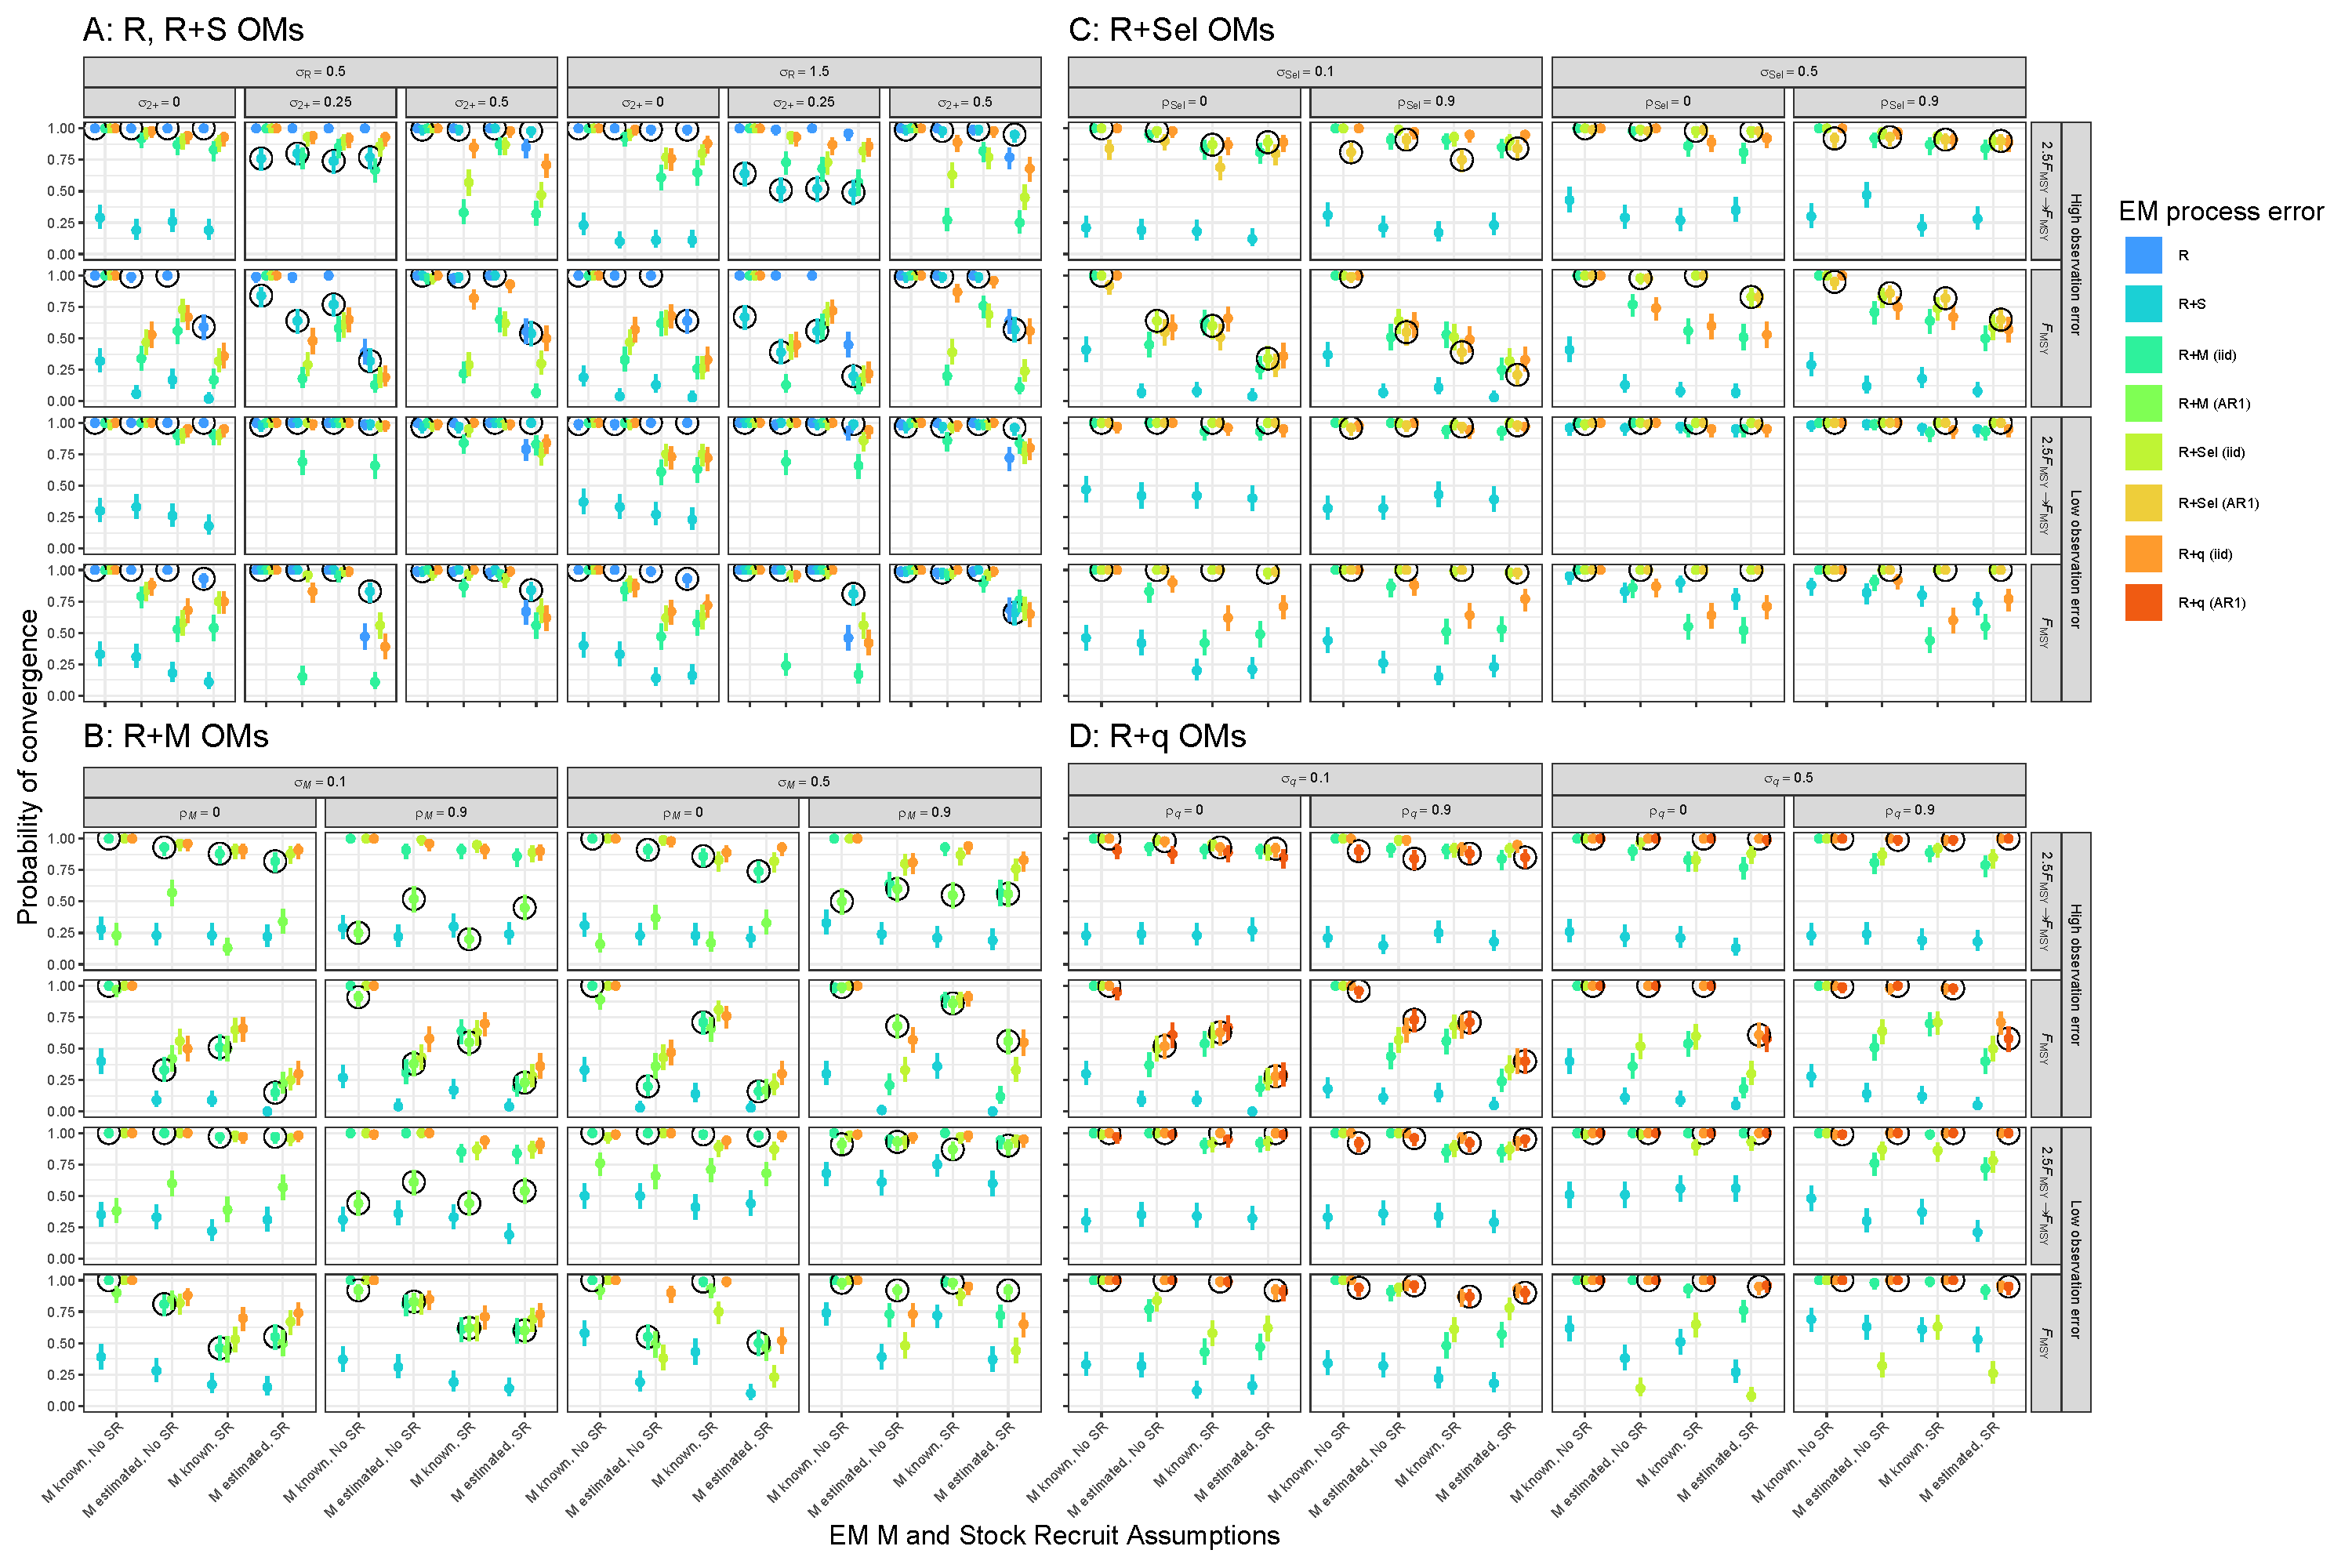
\includegraphics{type_4_convergence_plots}
%DIFDELCMD < %%%
\DIFdelendFL \DIFaddbeginFL 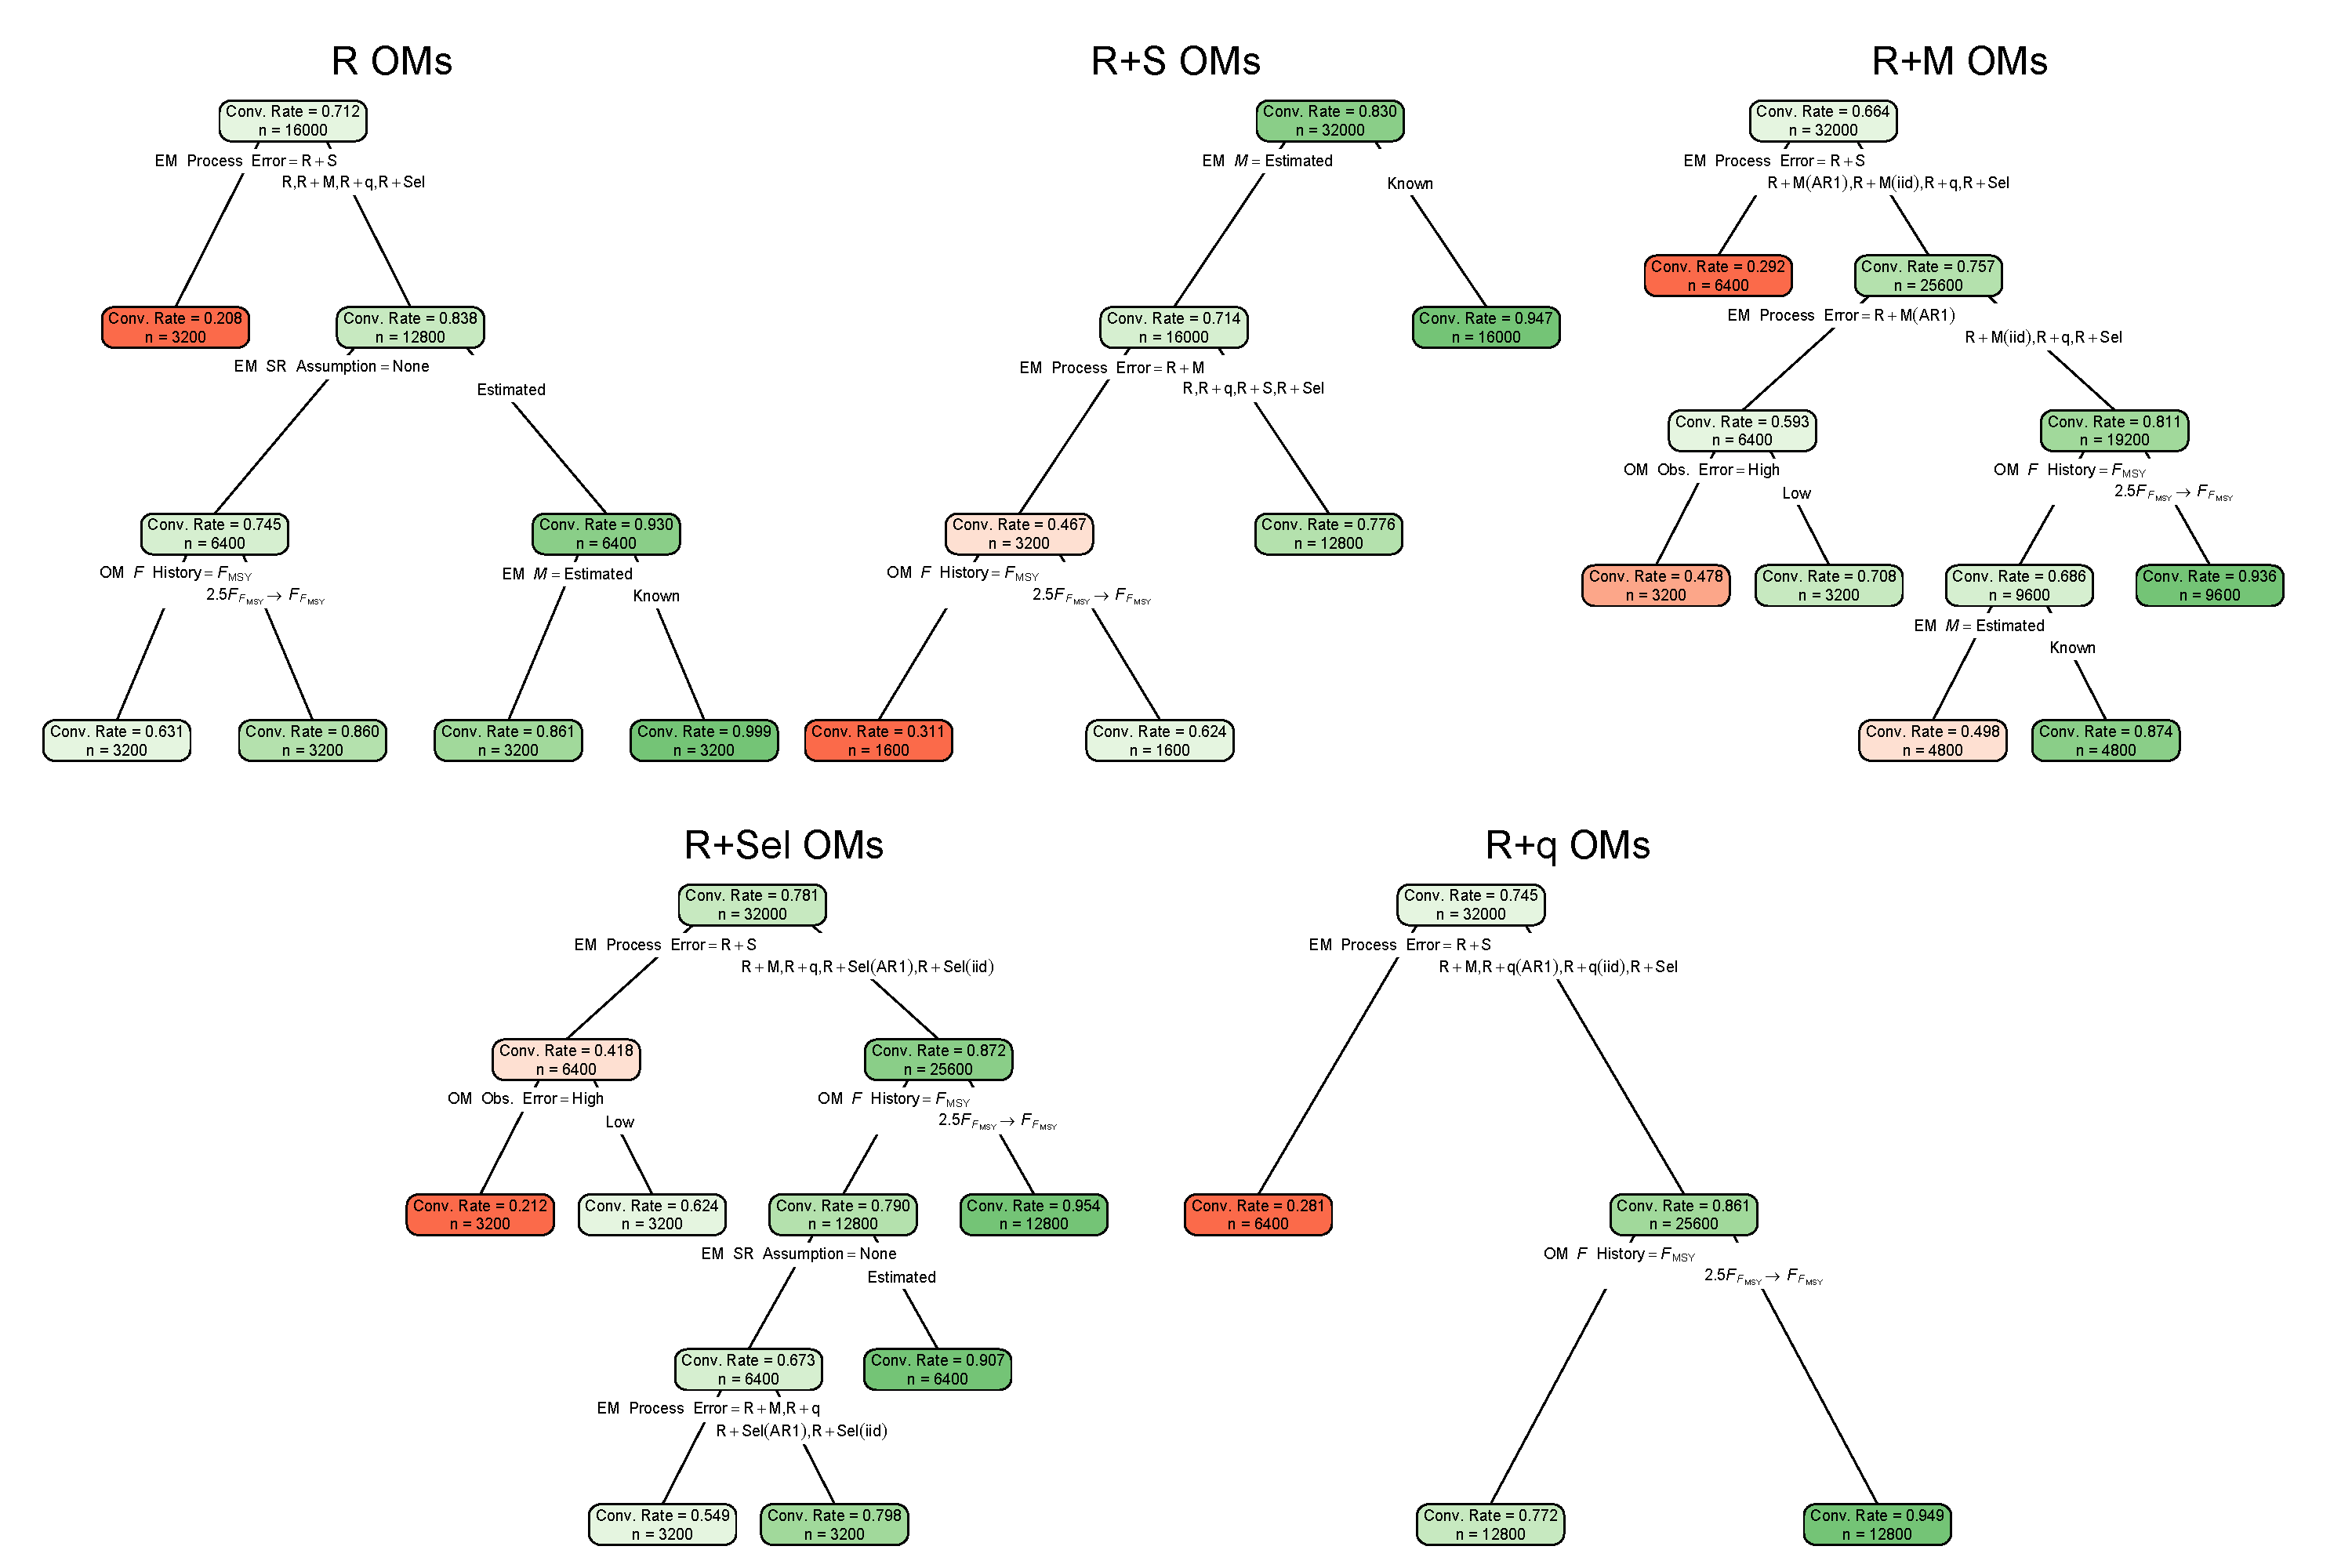
\includegraphics[width = 1.4\textwidth]{convergence_classification_plots}
\DIFaddendFL \end{center}
\caption{\DIFdelbeginFL \DIFdelFL{Estimated probability of fits }\DIFdelendFL \DIFaddbeginFL \DIFaddFL{Classification trees indicating primary factors determining convergence as defined by }\DIFaddendFL providing hessian-based standard errors for \DIFdelbeginFL \DIFdelFL{EMs assuming alternative process error (colored points and lines)}\DIFdelendFL \DIFaddbeginFL \DIFaddFL{R}\DIFaddendFL , \DIFdelbeginFL \DIFdelFL{and median natural mortality (estimated or known) and Beverton-Holt stock-recruit relationships (estimated or not; along x-axis) when fitted to operating models that have }\DIFdelendFL R\DIFdelbeginFL \DIFdelFL{and R}\DIFdelendFL +S\DIFdelbeginFL \DIFdelFL{(A)}\DIFdelendFL , R+\DIFdelbeginFL \DIFdelFL{Sel (B)}\DIFdelendFL \DIFaddbeginFL \DIFaddFL{M}\DIFaddendFL , R+\DIFdelbeginFL \DIFdelFL{M (C), or }\DIFdelendFL \DIFaddbeginFL \DIFaddFL{Sel and }\DIFaddendFL R+q \DIFdelbeginFL \DIFdelFL{(D) process error structures}\DIFdelendFL \DIFaddbeginFL \DIFaddFL{OMs}\DIFaddendFL . \DIFdelbeginFL \DIFdelFL{Circled values indicate results where the EM process error structure matches that of the operating model and vertical lines represent 95\% confidence intervals.}\DIFdelendFL \DIFaddbeginFL \DIFaddFL{Lower or higher convergence rates are indicated by more red or green polygons, respectively}\DIFaddendFL }\DIFdelbeginFL %DIFDELCMD < \label{hessian_SE_convergence}
%DIFDELCMD < %%%
\DIFdelendFL \DIFaddbeginFL \label{conv_class}
\DIFaddendFL \end{figure}
\end{landscape}

\DIFdelbegin %DIFDELCMD < \clearpage
%DIFDELCMD < %%%
\DIFdelend \DIFaddbegin \begin{landscape}
\begin{figure}
\begin{center}
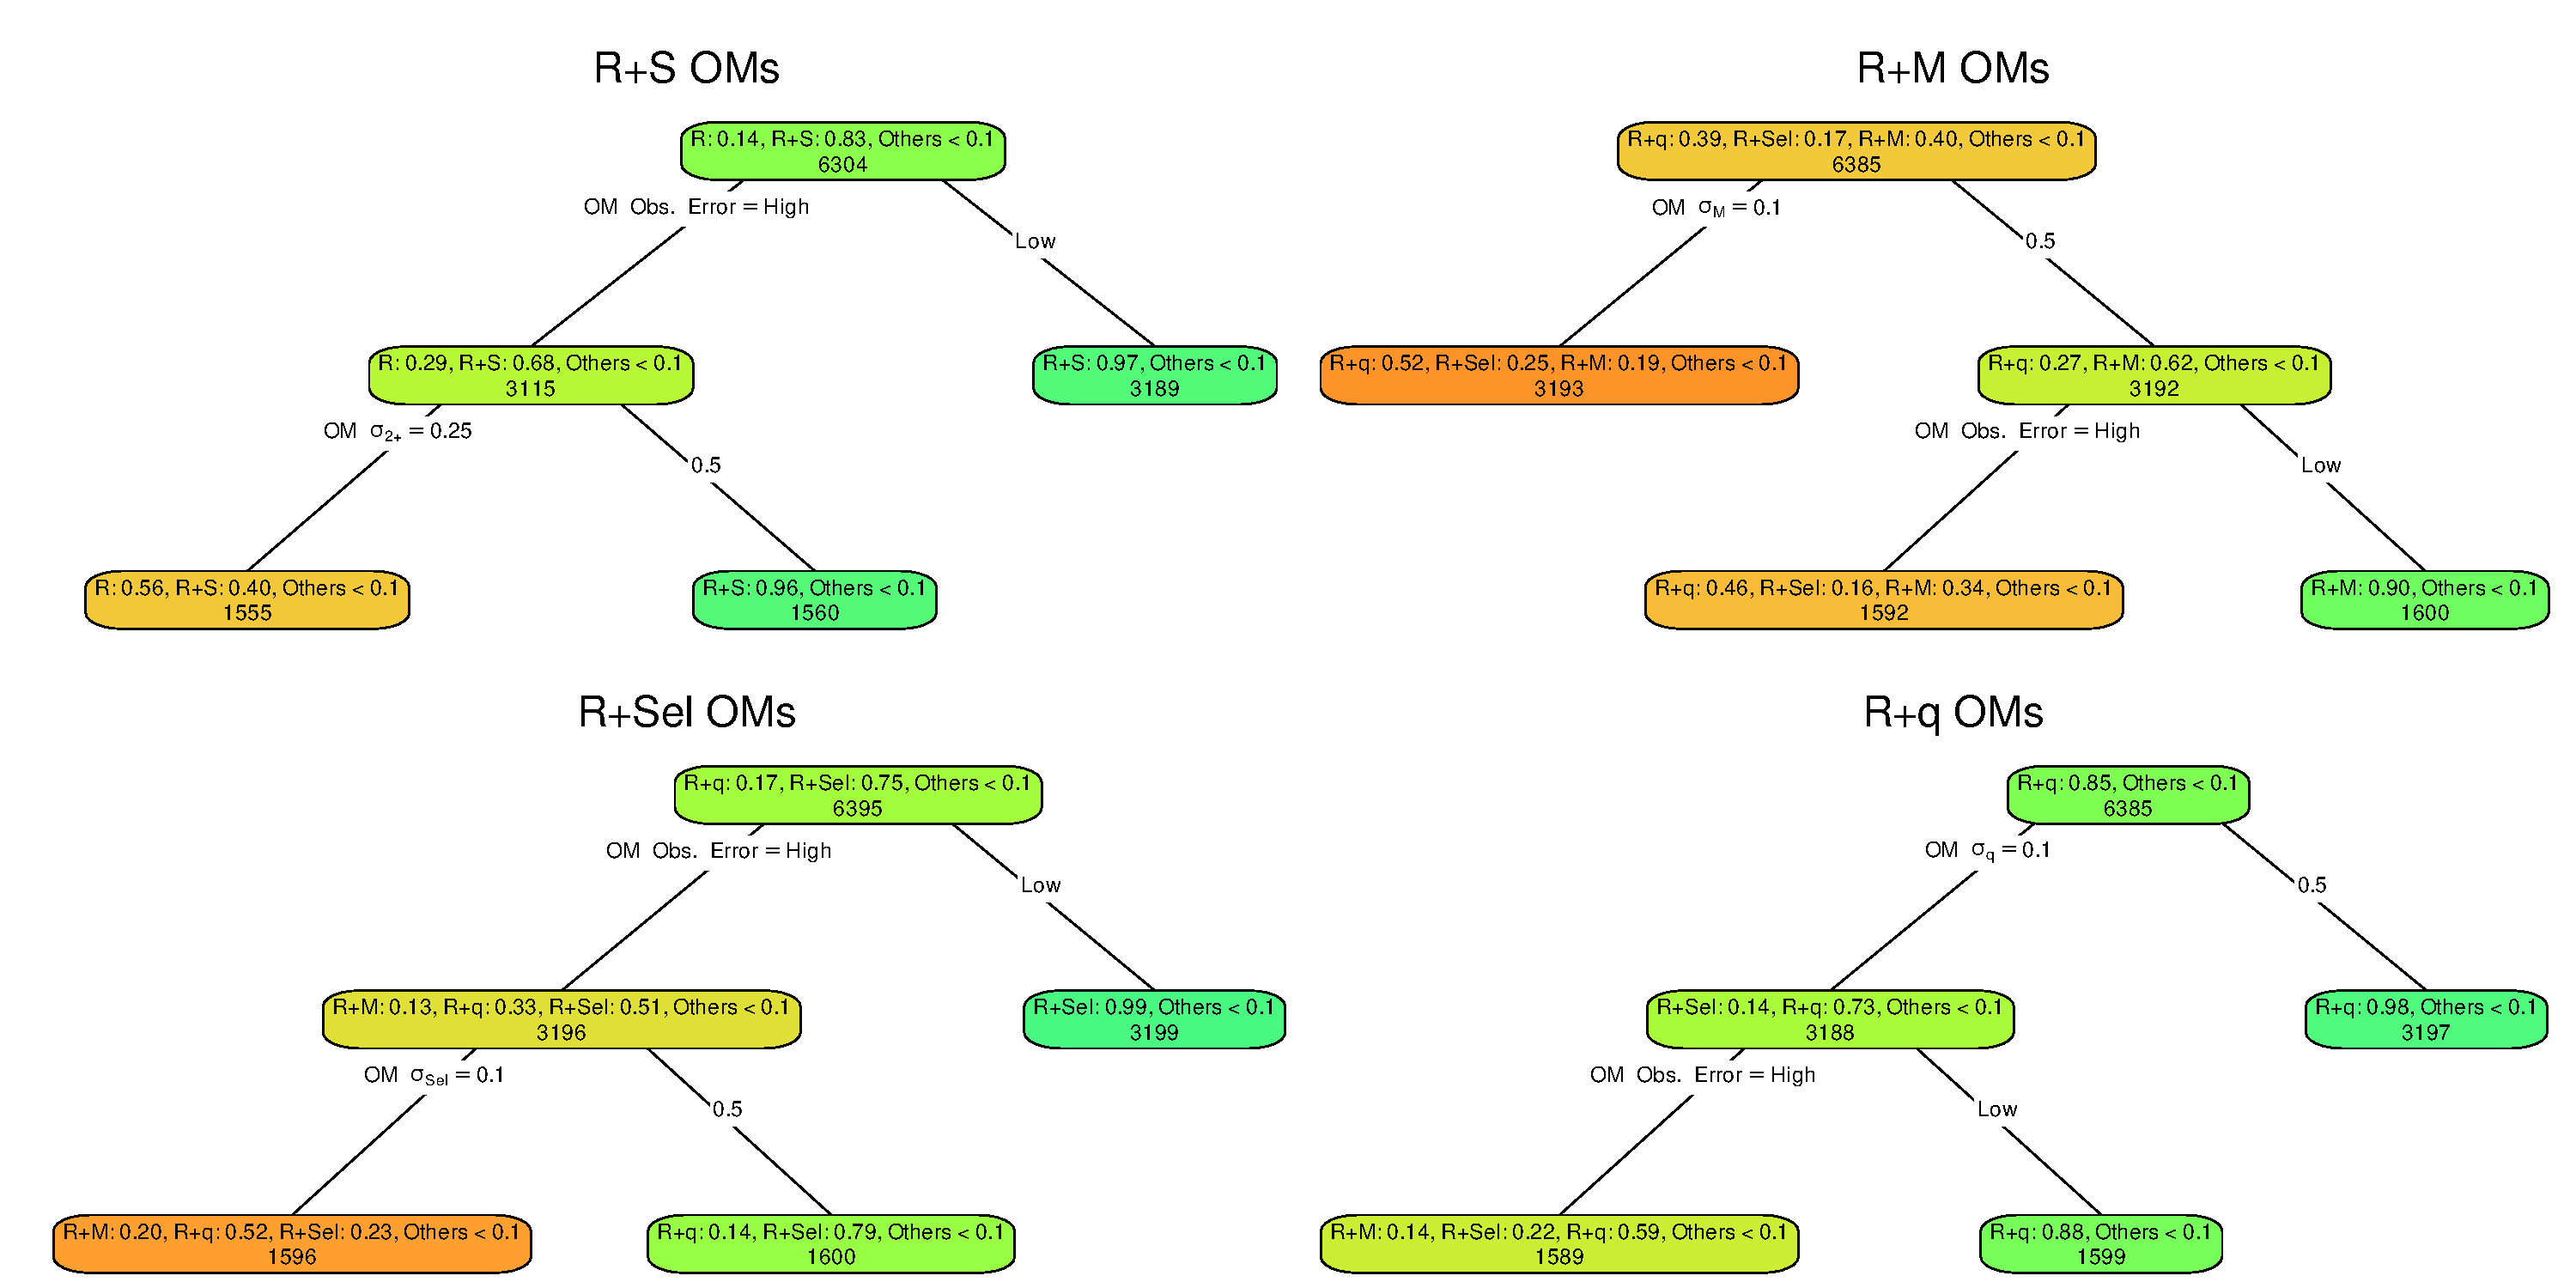
\includegraphics[width = 1.4\textwidth]{AIC_PE_classification_plots}
\end{center}
\caption{\DIFaddFL{Classification trees indicating primary factors determining which EM process error assumption provides the lowest AIC for R+S, R+M, R+Sel and R+q OMs. Each node shows the proportion of EM process error models with lowest AIC (top) and number of observations (bottom) for the corresponding subset. Lower or higher accuracy of the process error assumption are indicated by more red or green polygons, respectively.}}\label{AIC_PE_class}
\end{figure}
\end{landscape}
\DIFaddend 

\begin{landscape}
\begin{figure}
\begin{center}
\DIFdelbeginFL %DIFDELCMD < 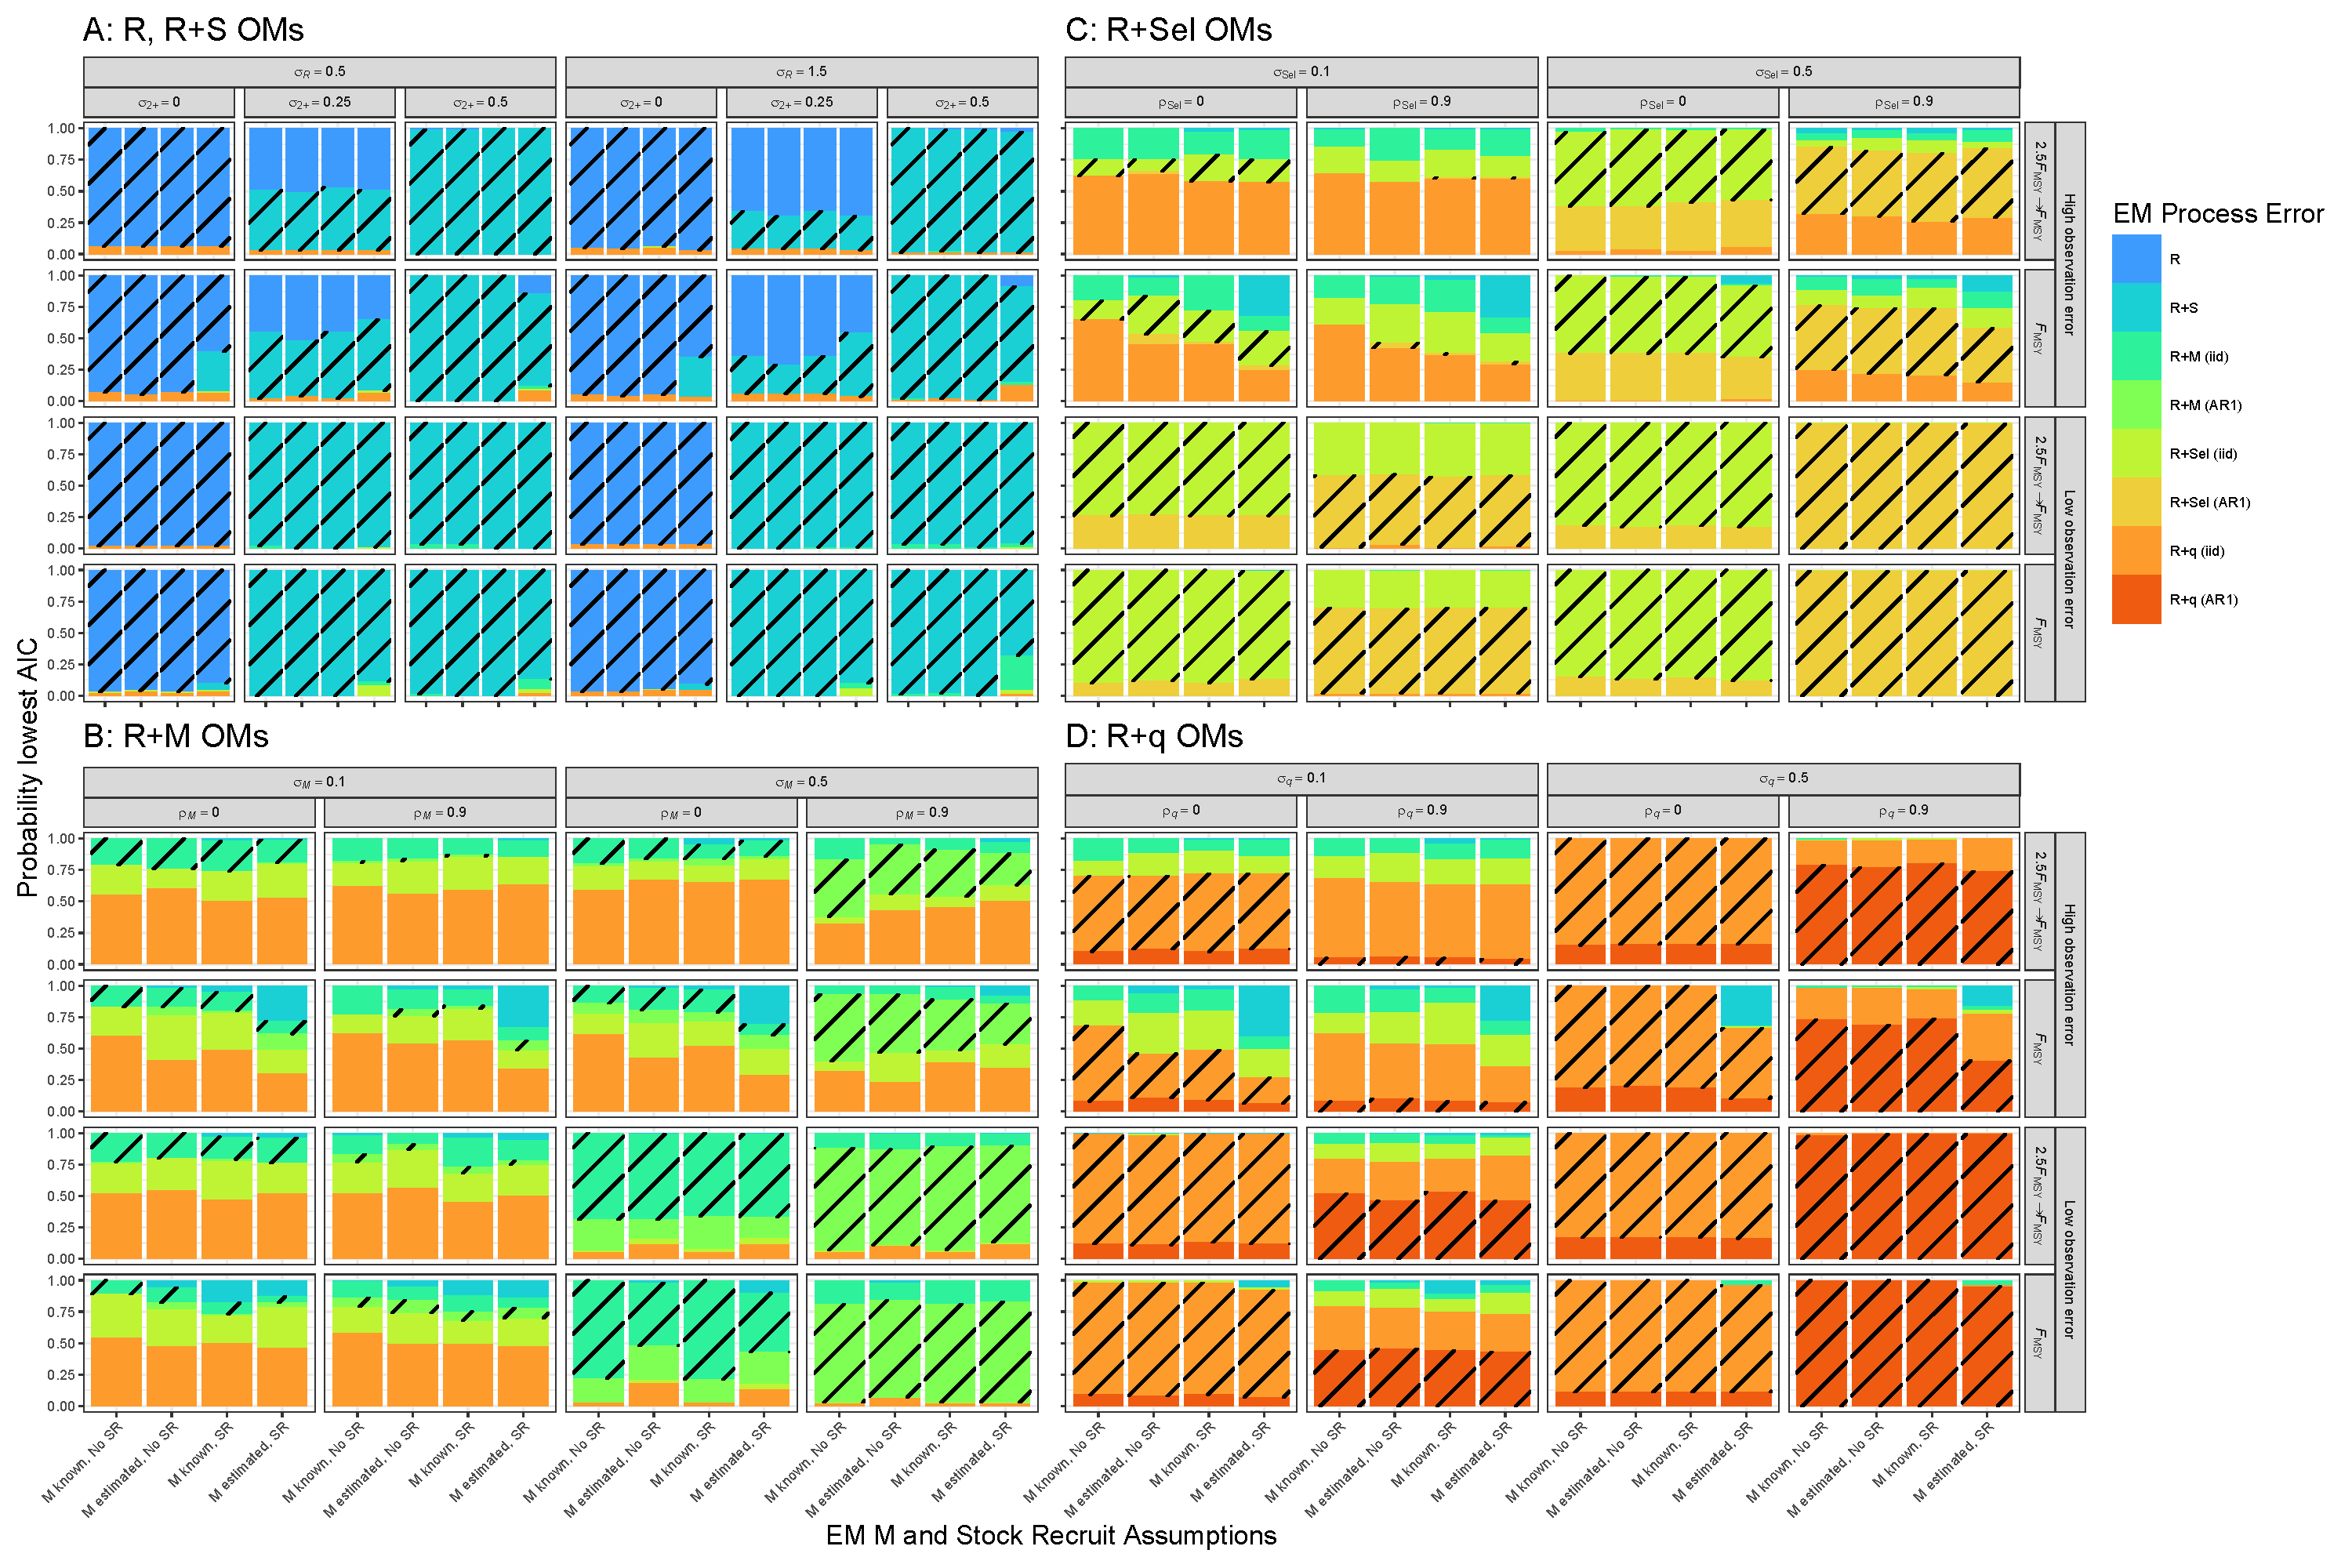
\includegraphics{pe_aic_plots}
%DIFDELCMD < %%%
\DIFdelendFL \DIFaddbeginFL 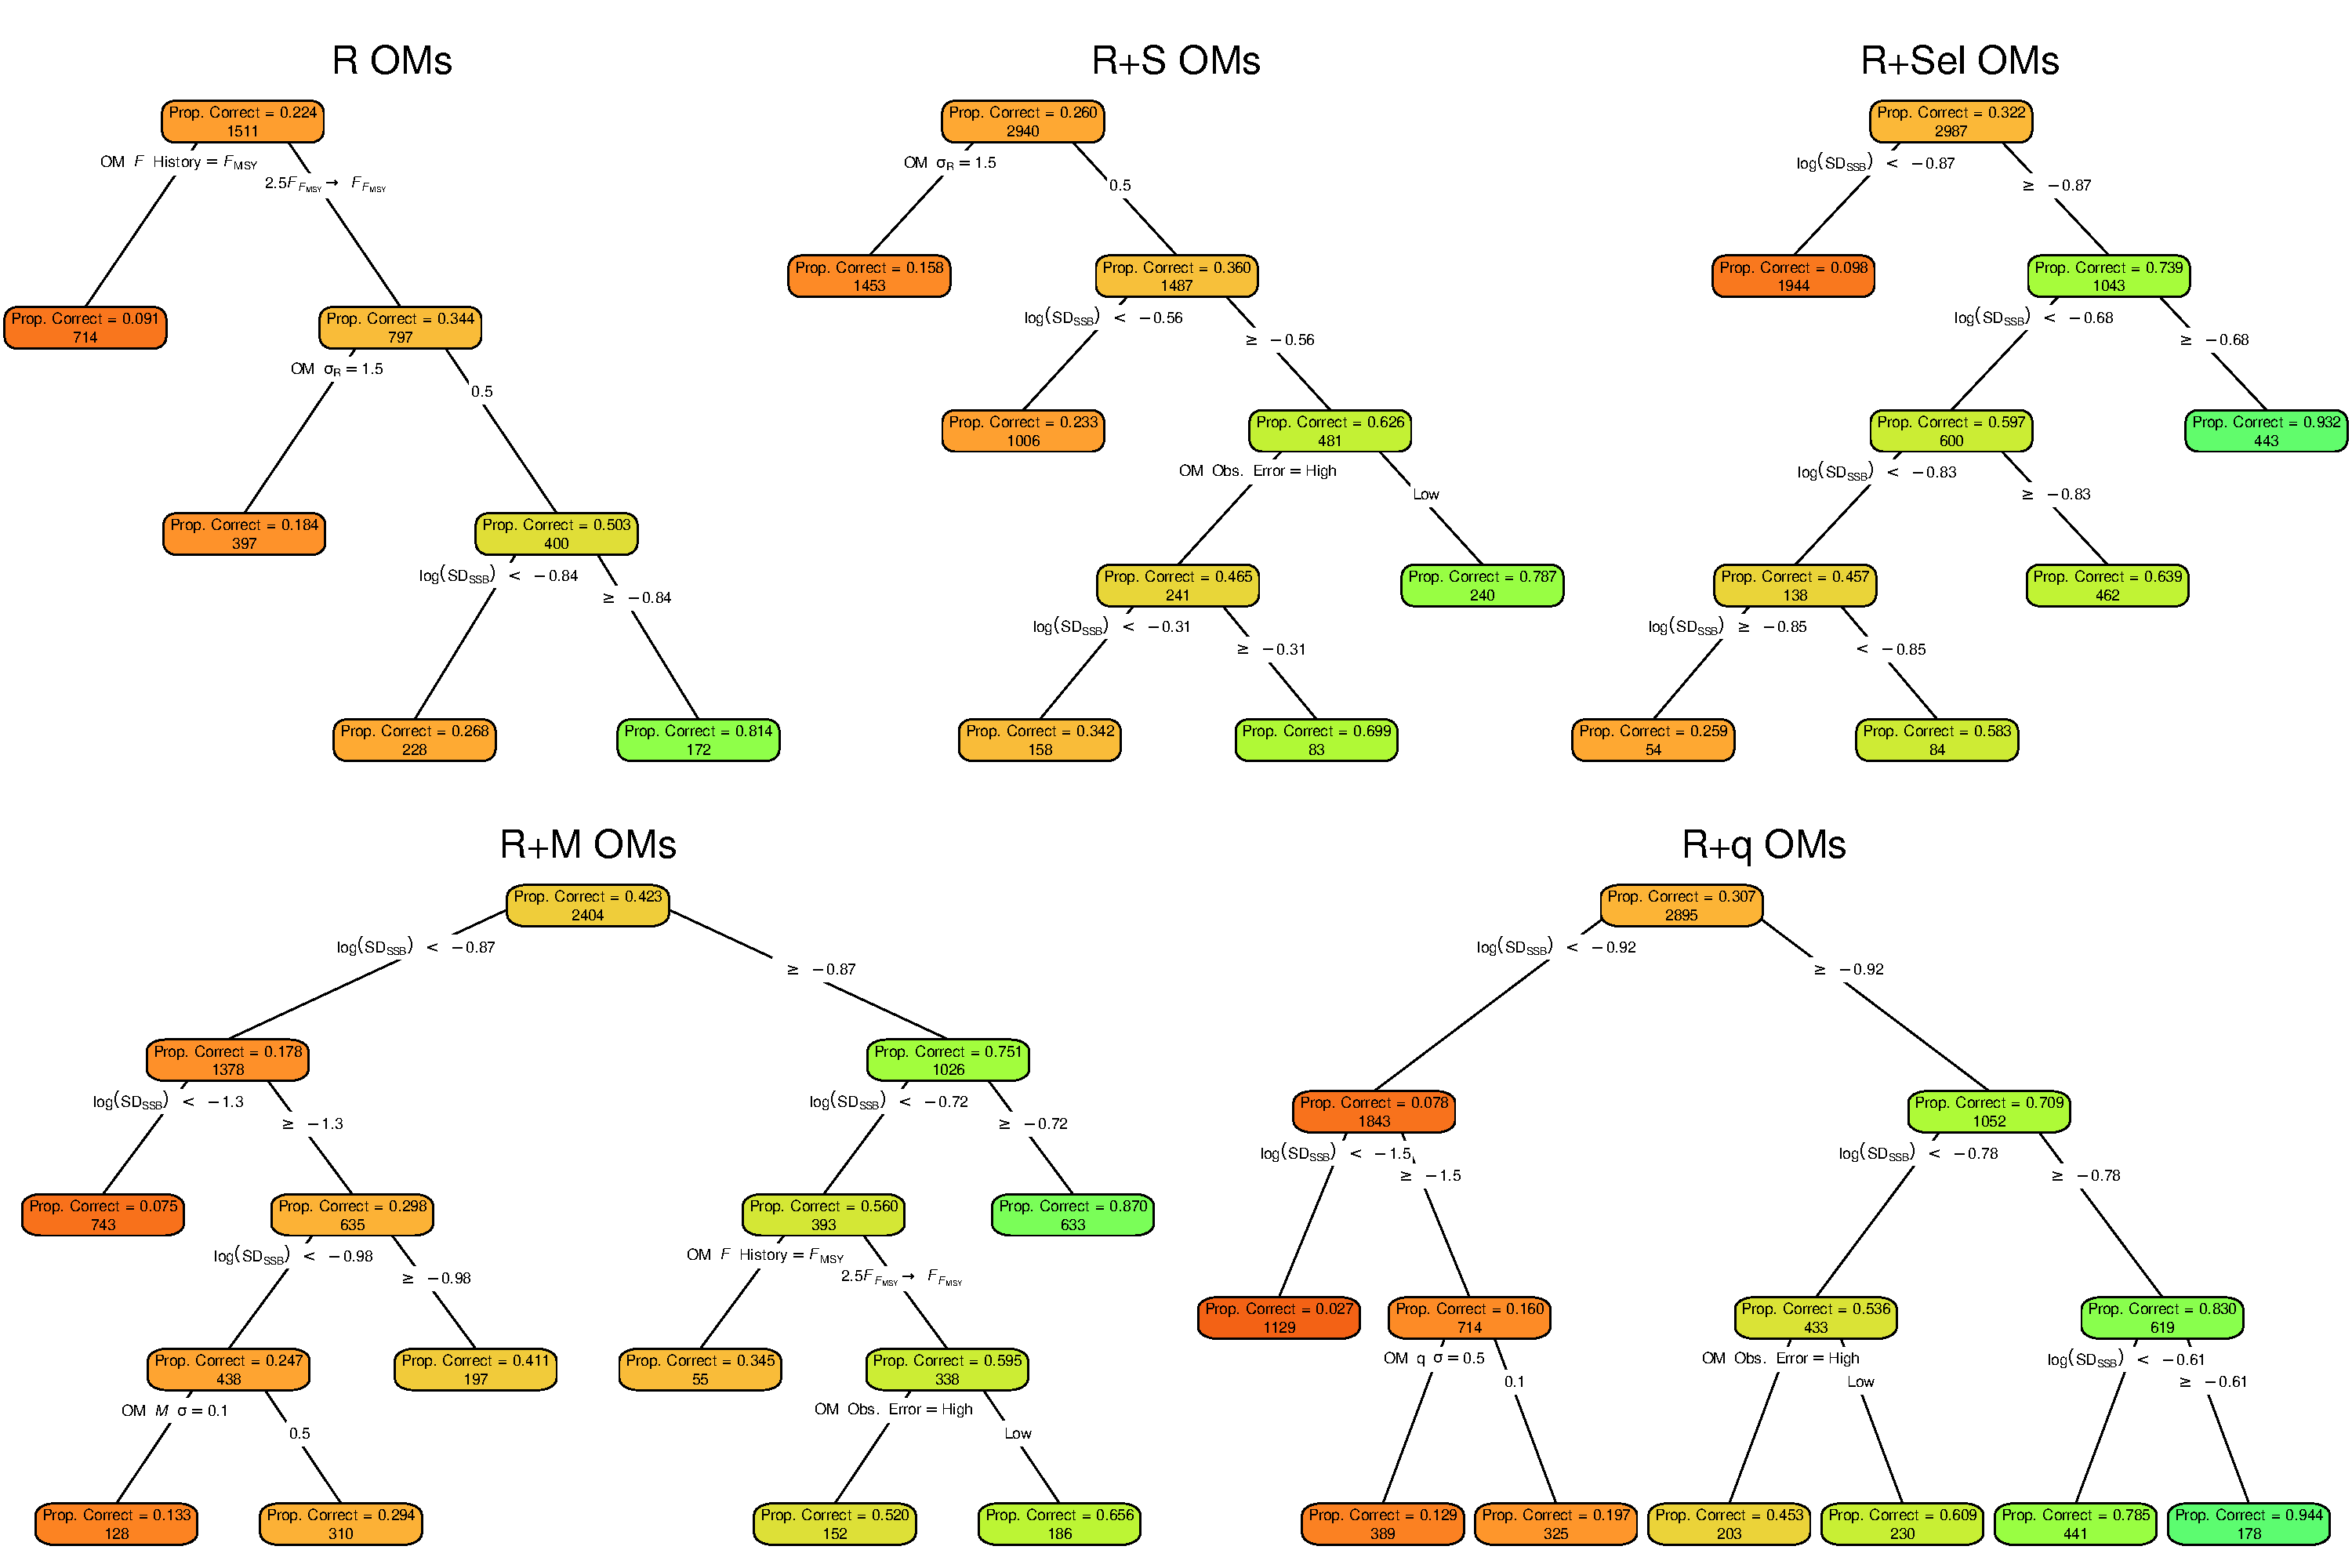
\includegraphics[width = 1.4\textwidth]{AIC_SRR_classification_plots}
\DIFaddendFL \end{center}
\caption{\DIFdelbeginFL \DIFdelFL{Estimated probability of lowest AIC for EMs assuming alternative process error structures }\DIFdelendFL \DIFaddbeginFL \DIFaddFL{Classification trees indicating primary factors determining which EM stock recruitment assumption }\DIFaddendFL (\DIFdelbeginFL \DIFdelFL{colored bars) conditional on alternative assumptions for median natural mortality (estimated }\DIFdelendFL \DIFaddbeginFL \DIFaddFL{none }\DIFaddendFL or \DIFdelbeginFL \DIFdelFL{known) and }\DIFdelendFL Beverton-Holt\DIFdelbeginFL \DIFdelFL{stock-recruit relationships (estimated or not; along x-axis}\DIFdelendFL ) \DIFdelbeginFL \DIFdelFL{when fitted to operating models that have }\DIFdelendFL \DIFaddbeginFL \DIFaddFL{provides the lowest AIC for }\DIFaddendFL R\DIFdelbeginFL \DIFdelFL{and }\DIFdelendFL \DIFaddbeginFL \DIFaddFL{, }\DIFaddendFL R+S\DIFdelbeginFL \DIFdelFL{(A)}\DIFdelendFL , R+\DIFdelbeginFL \DIFdelFL{Sel (B)}\DIFdelendFL \DIFaddbeginFL \DIFaddFL{M}\DIFaddendFL , R+\DIFdelbeginFL \DIFdelFL{M (C), or }\DIFdelendFL \DIFaddbeginFL \DIFaddFL{Sel and }\DIFaddendFL R+q \DIFaddbeginFL \DIFaddFL{OMs. Each node shows the proportion of EMs that assume the stock-recruit relationship with lowest AIC }\DIFaddendFL (\DIFdelbeginFL \DIFdelFL{D}\DIFdelendFL \DIFaddbeginFL \DIFaddFL{top}\DIFaddendFL ) \DIFdelbeginFL \DIFdelFL{process error structures}\DIFdelendFL \DIFaddbeginFL \DIFaddFL{and number of observations (bottom) for the corresponding subset}\DIFaddendFL . \DIFdelbeginFL \DIFdelFL{Striped bars indicate results where }\DIFdelendFL \DIFaddbeginFL \DIFaddFL{Lower or higher accuracy of }\DIFaddendFL the \DIFdelbeginFL \DIFdelFL{EM }\DIFdelendFL process error \DIFdelbeginFL \DIFdelFL{structure matches that of the operating model}\DIFdelendFL \DIFaddbeginFL \DIFaddFL{assumption are indicated by more red or green polygons, respectively}\DIFaddendFL .}\DIFdelbeginFL %DIFDELCMD < \label{pe_aic}
%DIFDELCMD < %%%
\DIFdelendFL \DIFaddbeginFL \label{AIC_SRR_class}
\DIFaddendFL \end{figure}
\end{landscape}

\DIFdelbegin %DIFDELCMD < \clearpage
%DIFDELCMD < %%%
\DIFdelend \DIFaddbegin \begin{landscape}
\begin{figure}
\begin{center}
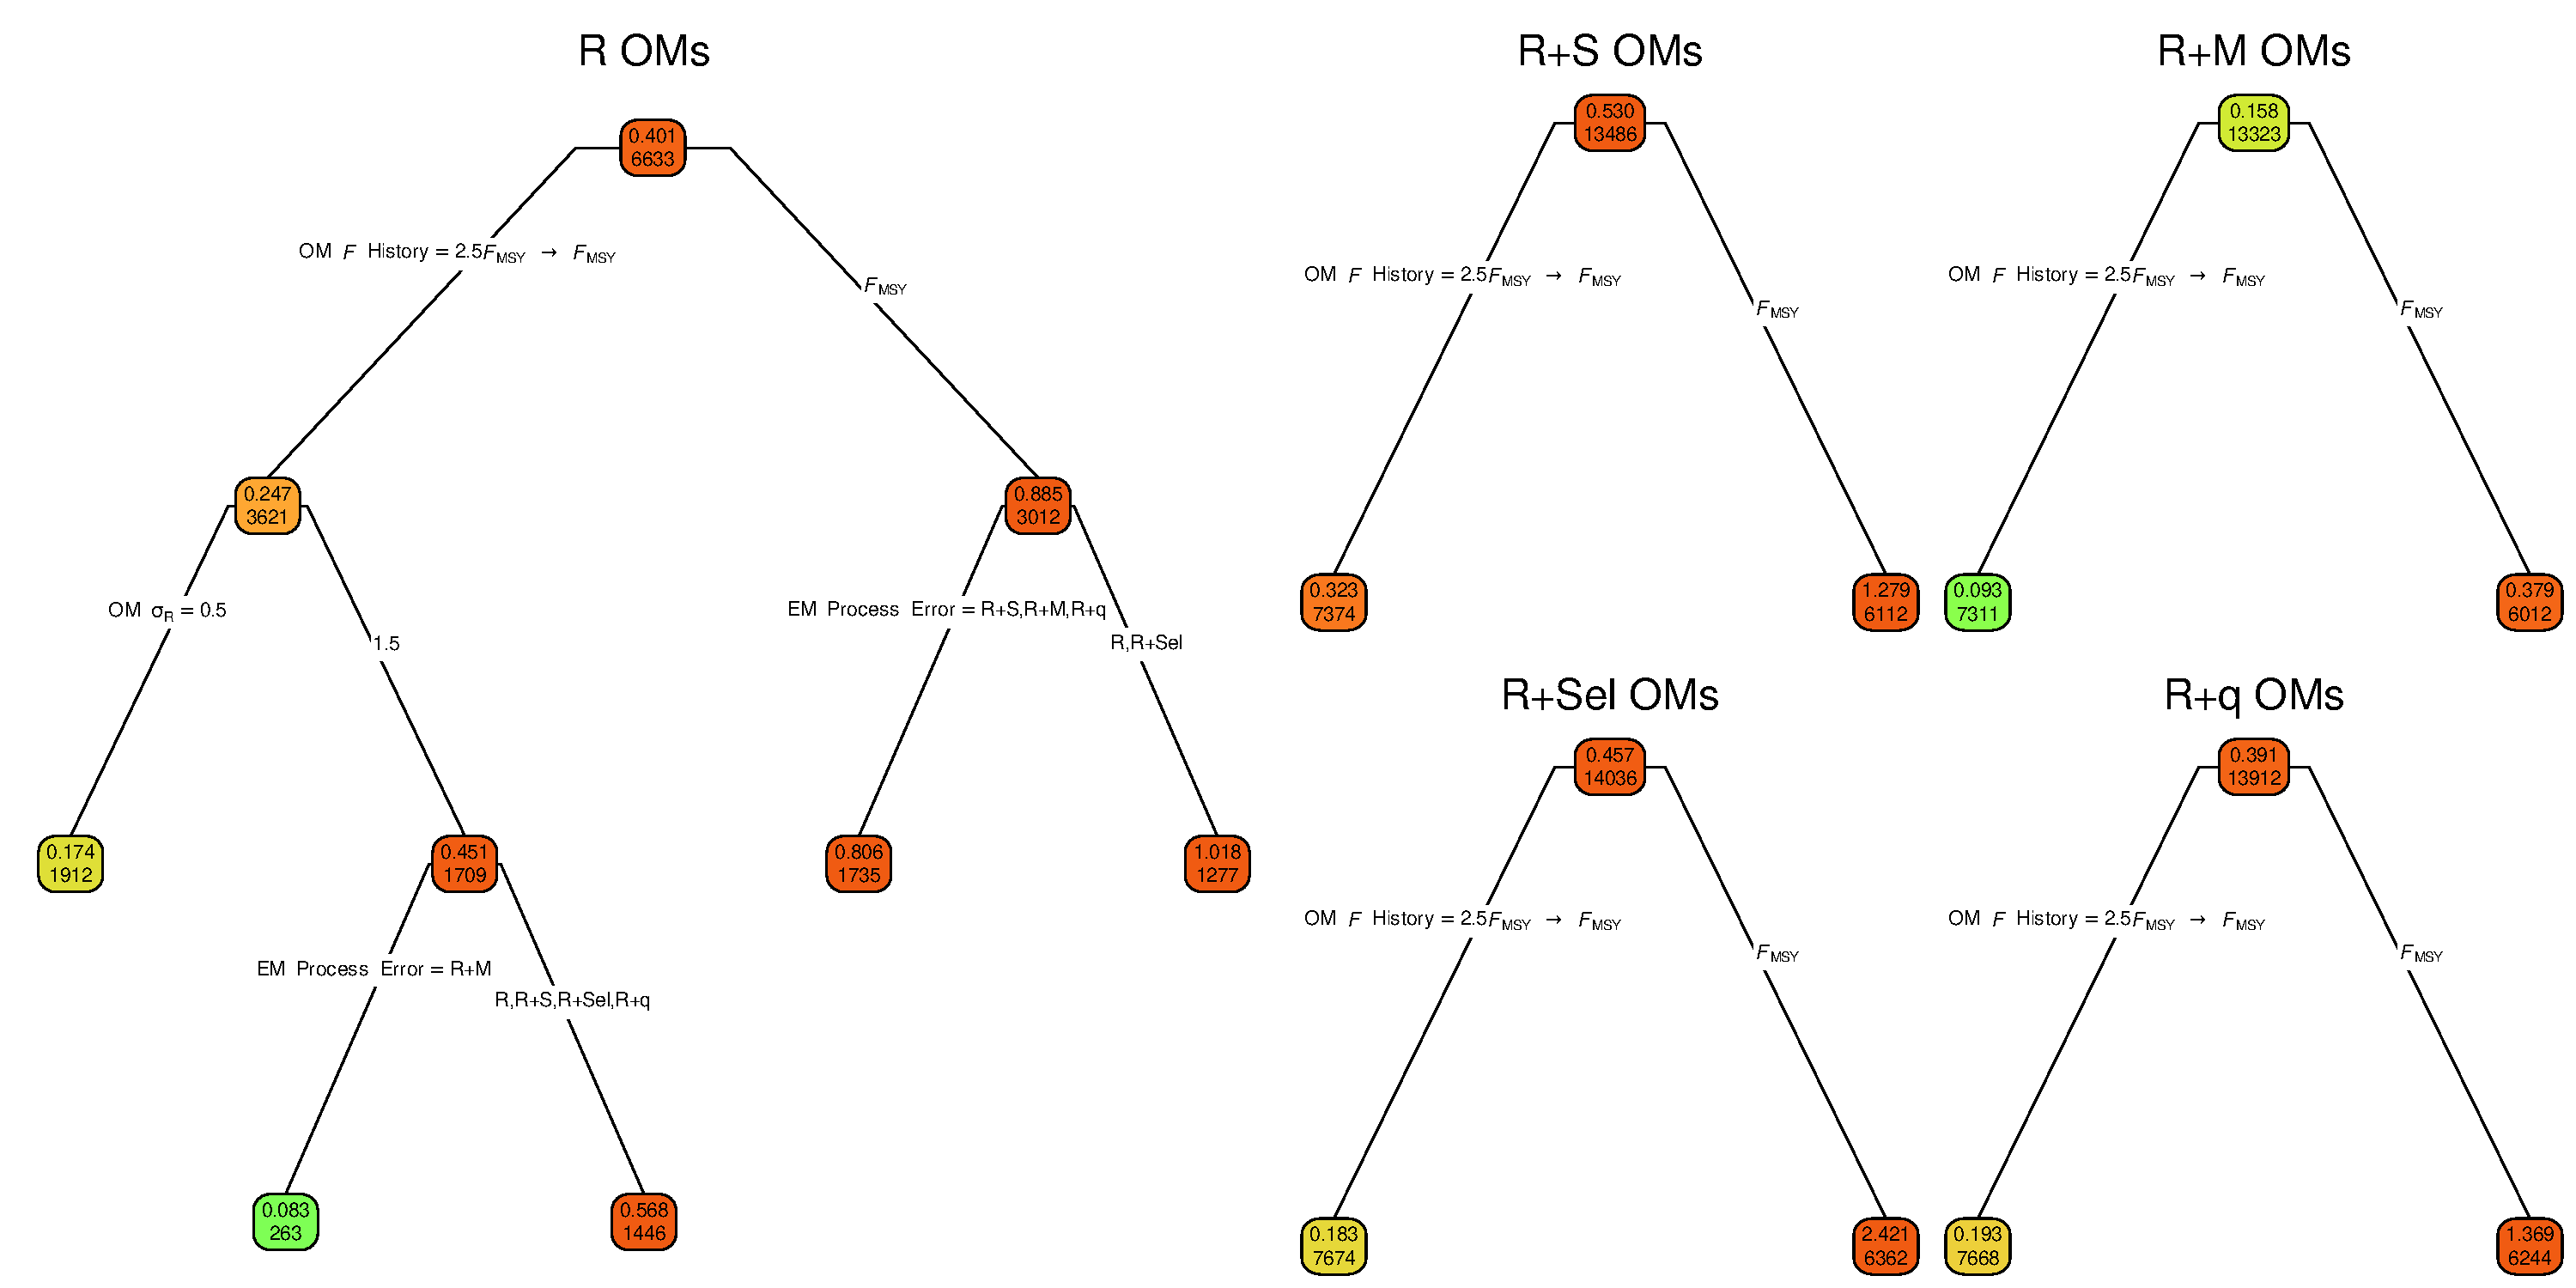
\includegraphics[width = 1.4\textwidth]{SR_a_bias_regtree_plots}
\end{center}
\caption{\DIFaddFL{Regression trees indicating primary factors determining reductions in sums of squares of errors in estimation measured by Eq. \ref{bias_regression_response} for the Beverton-Holt stock-recruit parameter $a$ for R+S, R+M, R+Sel and R+q OMs. Each node shows the median error (top) and number of observations (bottom) for the corresponding subset. Lower or higher median absolute errors of the process error assumption are indicated by more green or red polygons, respectively.}}\label{SR_a_bias_regtree}
\end{figure}
\end{landscape}
\DIFaddend 

\begin{landscape}
\begin{figure}
\begin{center}
\DIFdelbeginFL %DIFDELCMD < 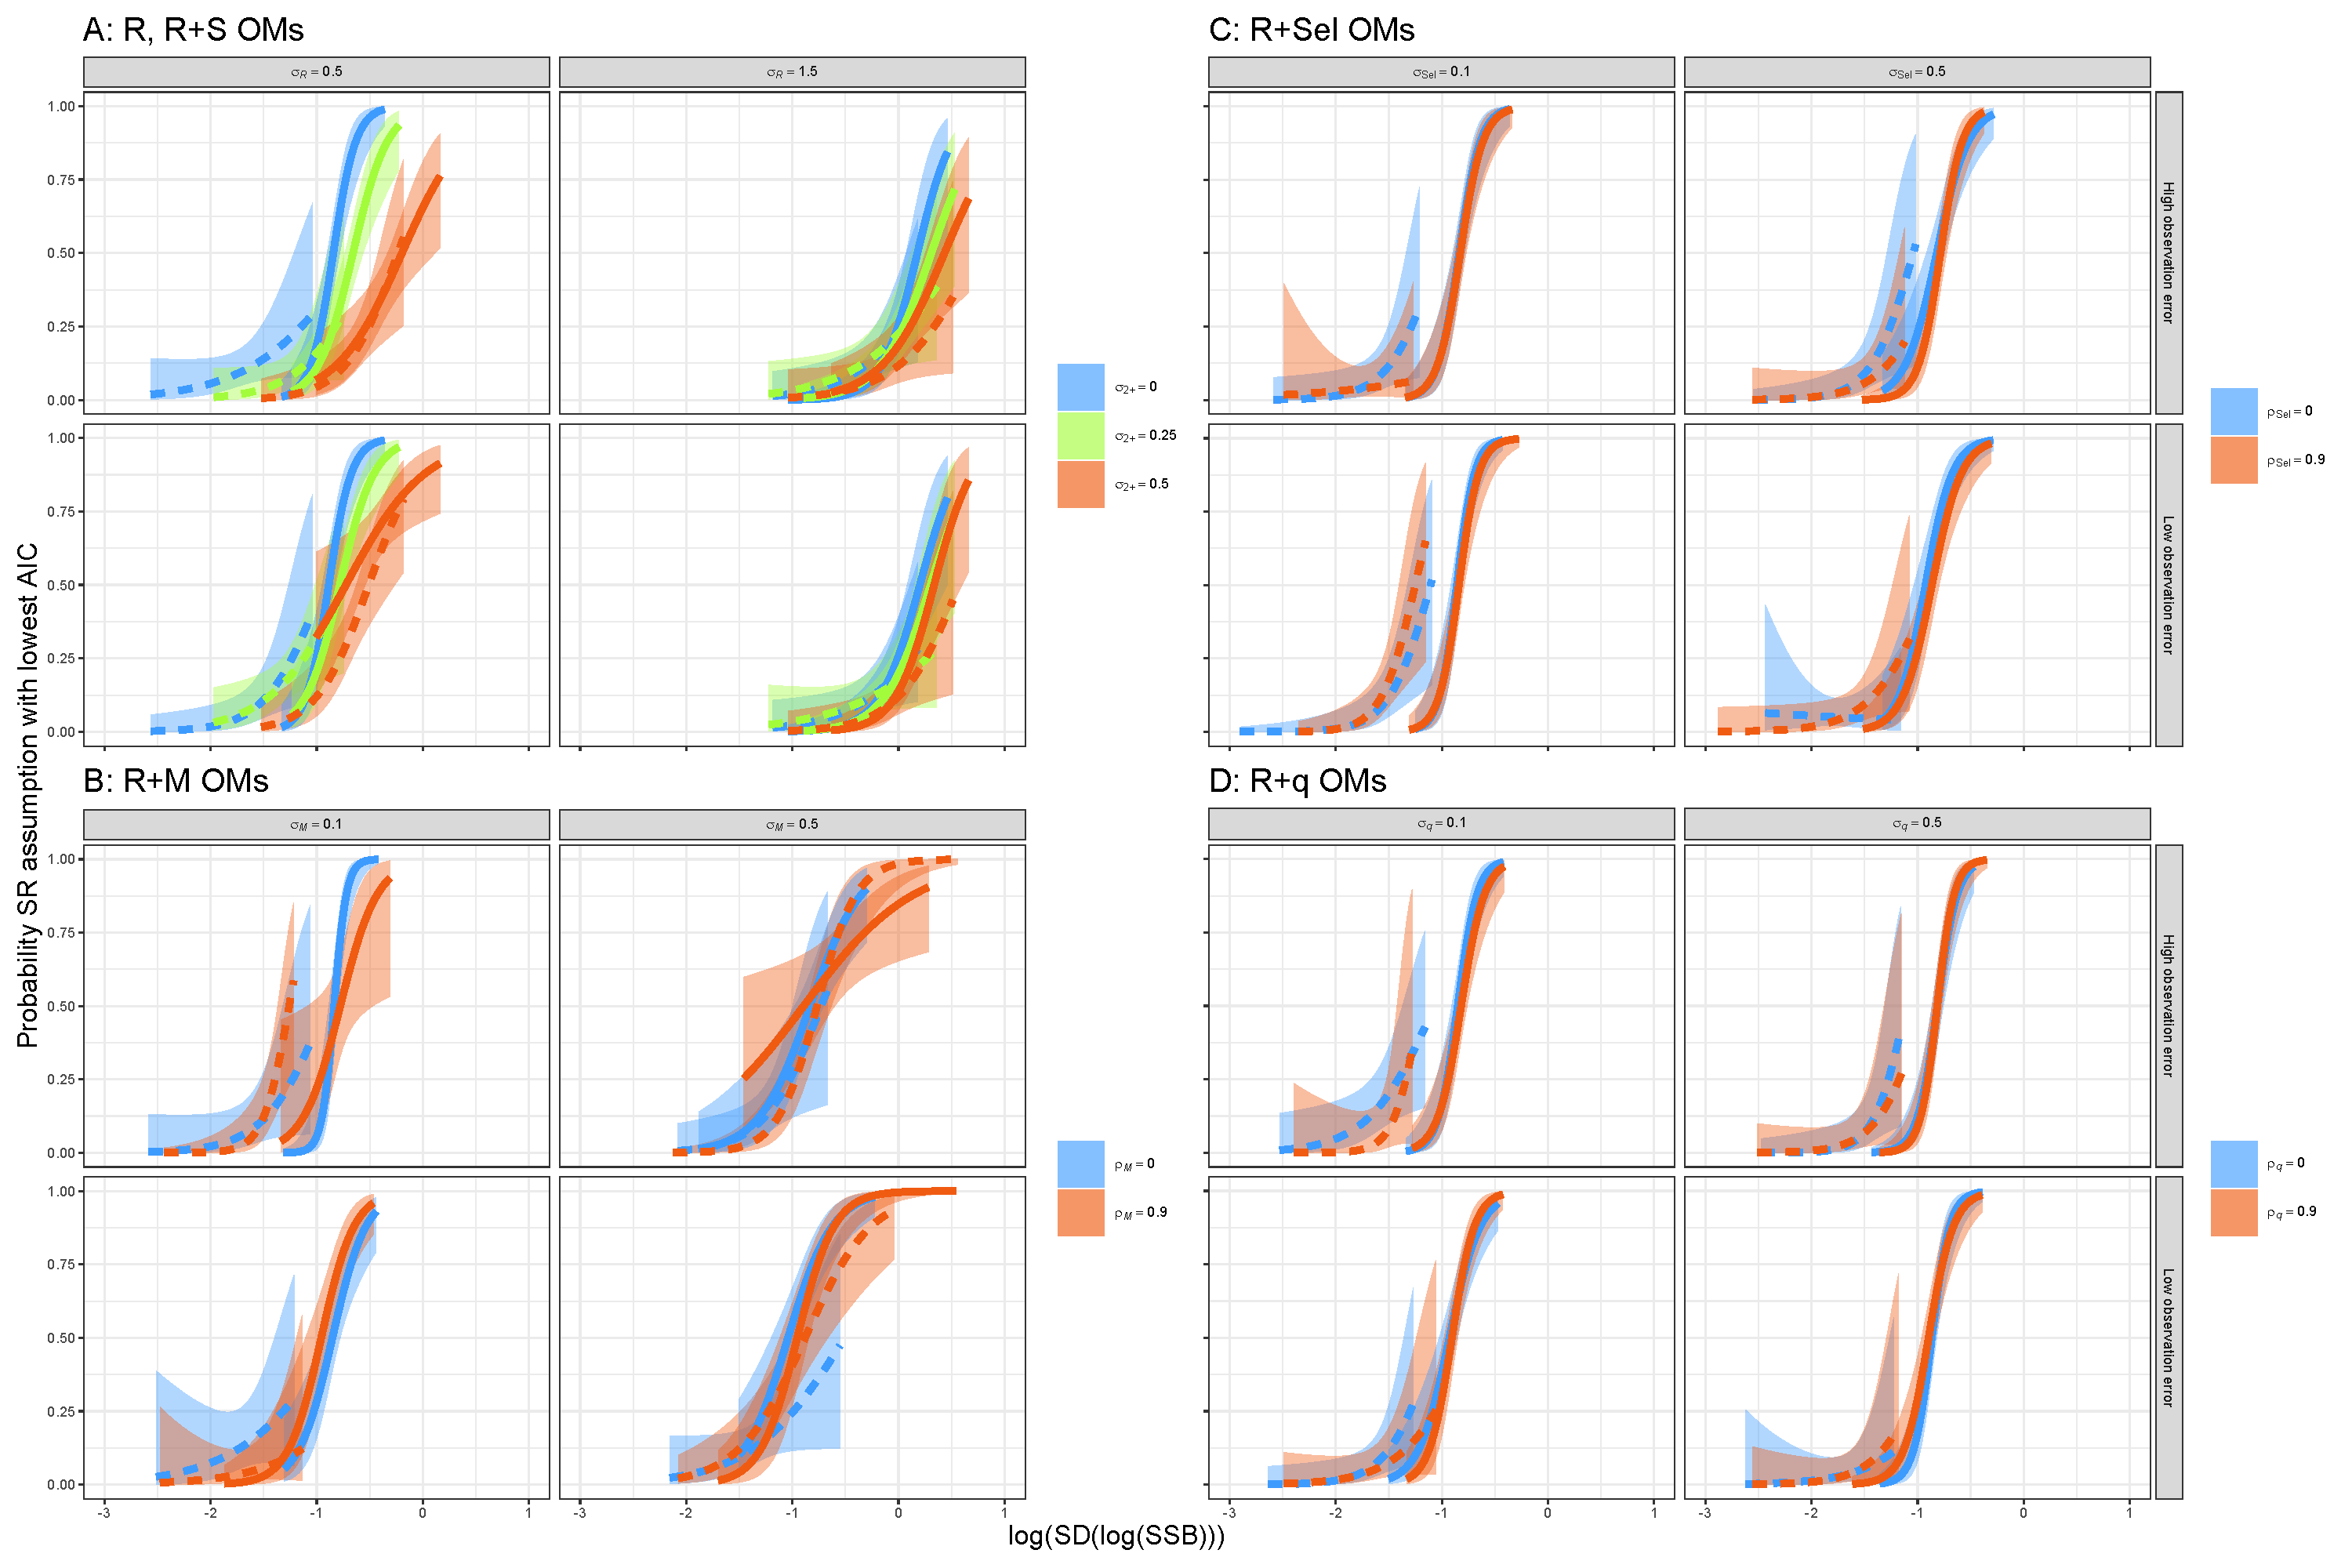
\includegraphics[height = 0.8\textheight]{sr_aic_plots_rev}
%DIFDELCMD < %%%
\DIFdelendFL \DIFaddbeginFL 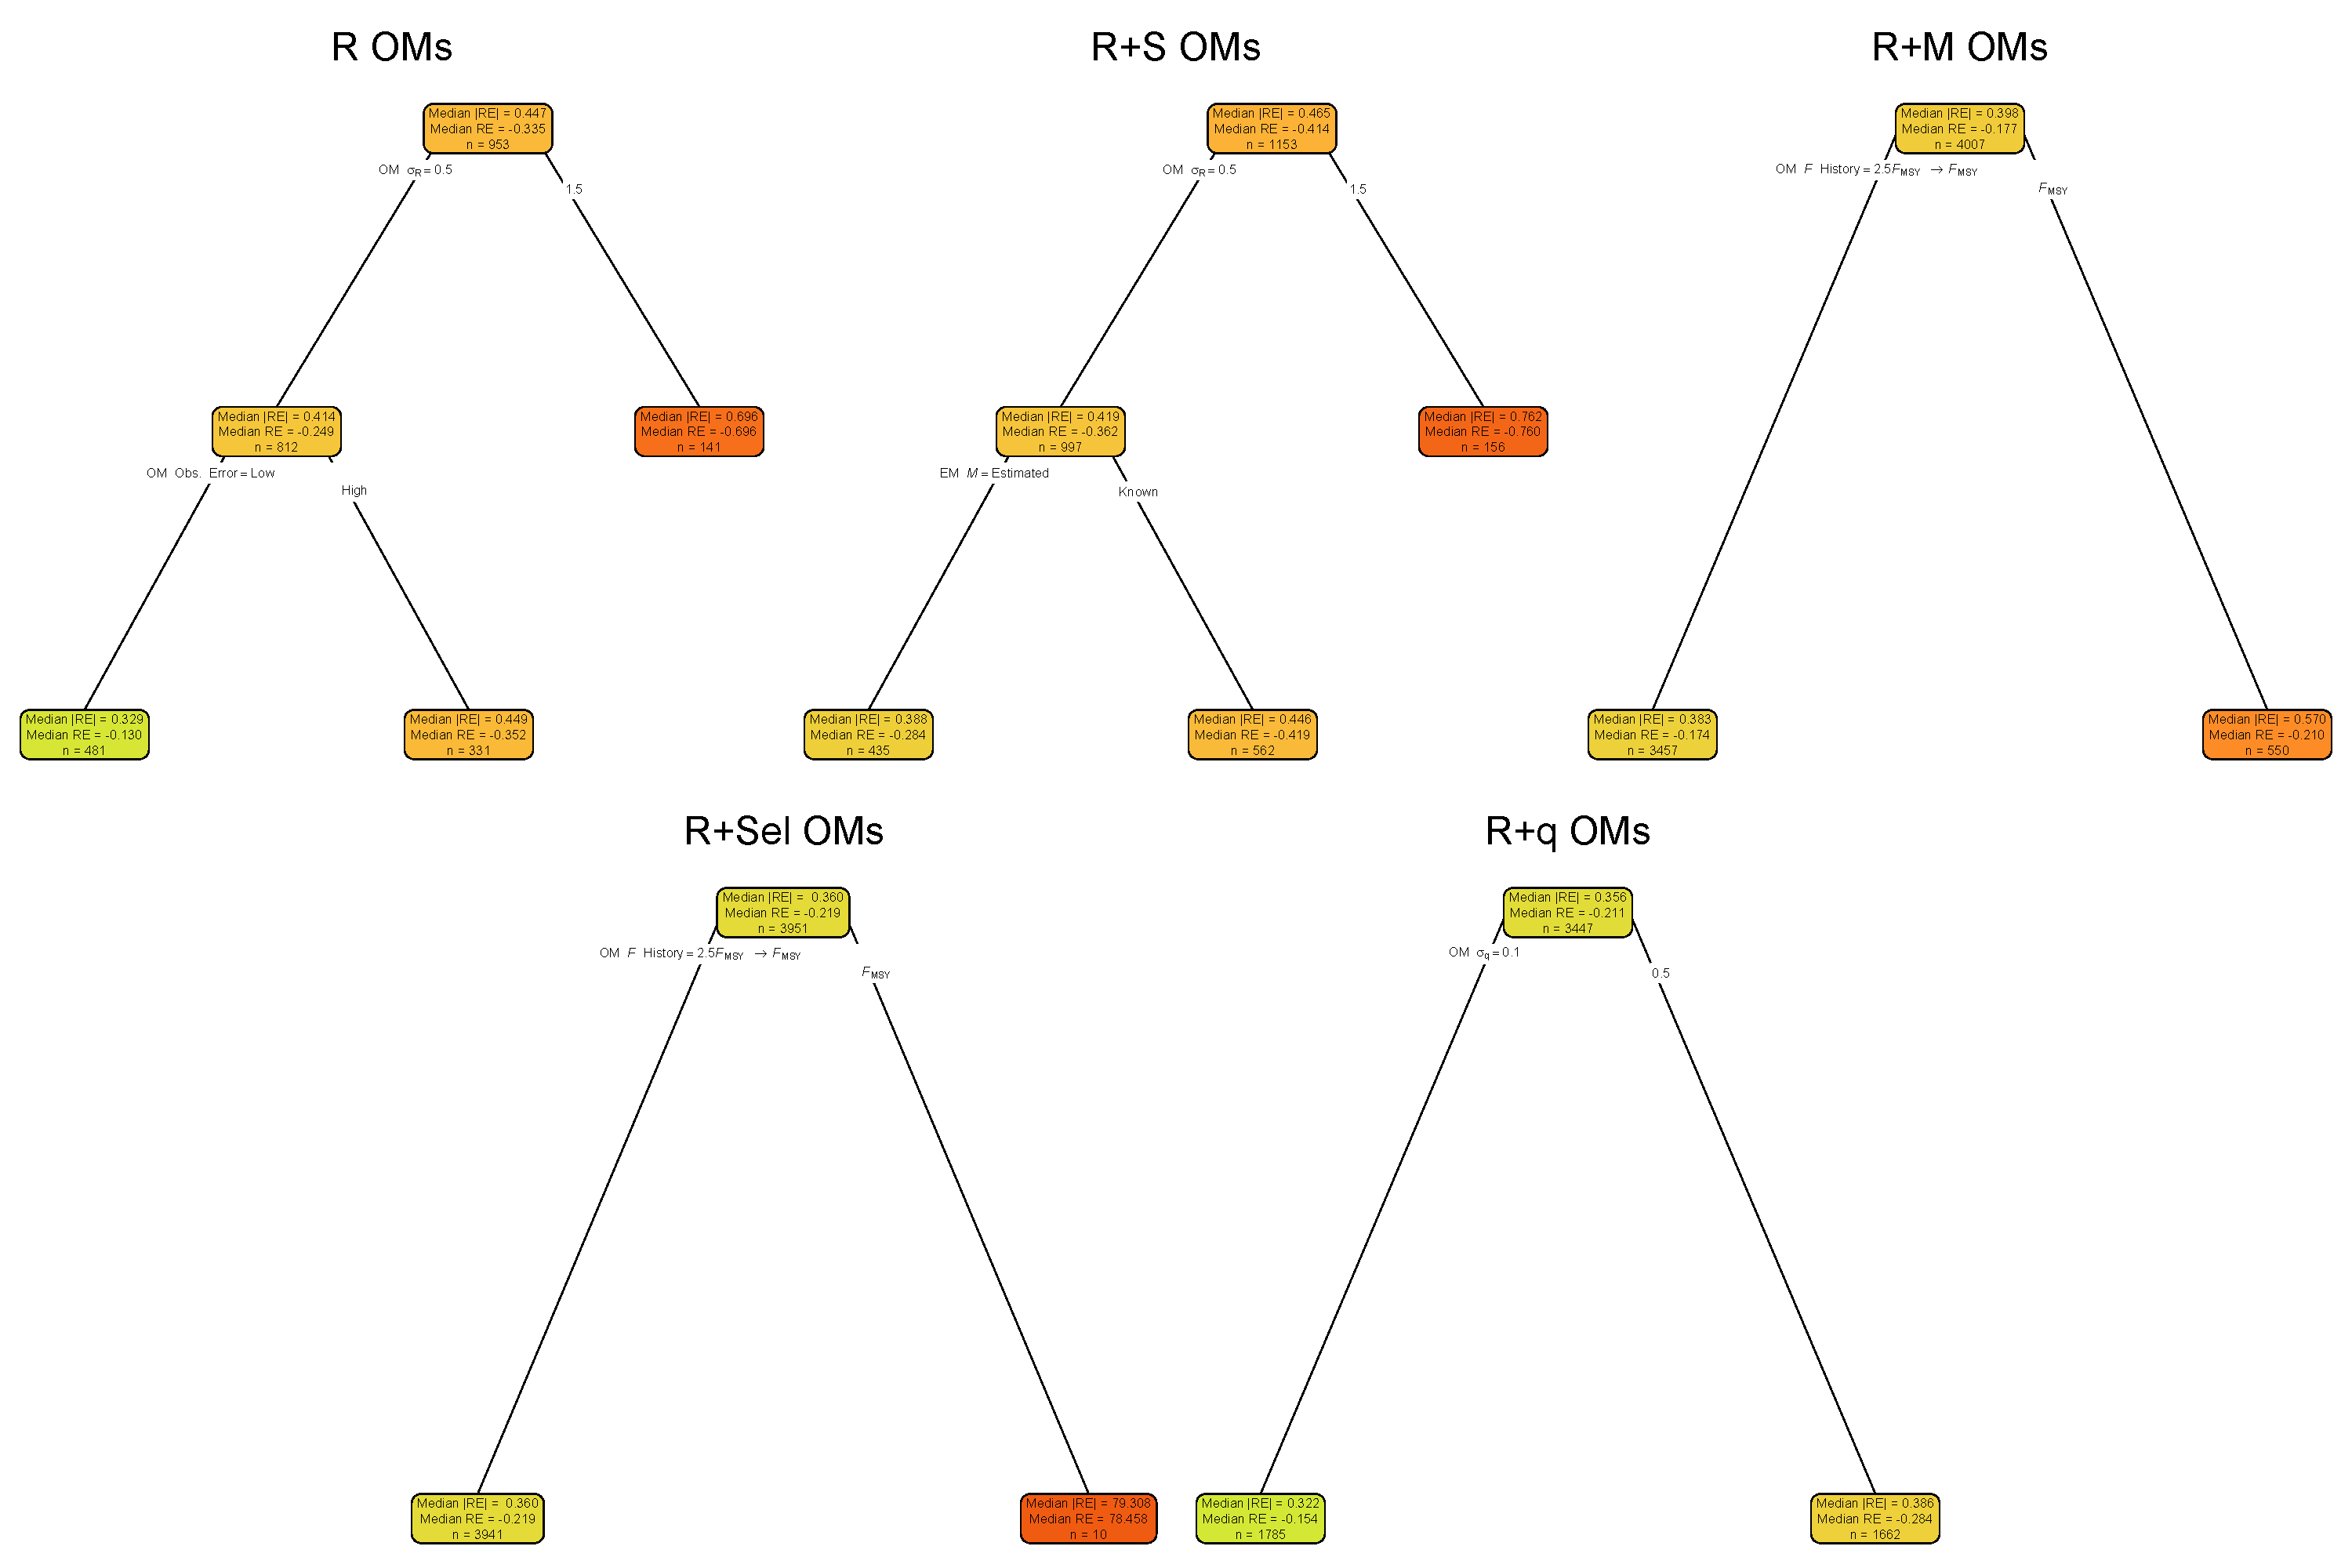
\includegraphics[width = 1.4\textwidth]{SR_b_bias_regtree_plots}
\DIFaddendFL \end{center}
\caption{\DIFdelbeginFL \DIFdelFL{Estimated probability }\DIFdelendFL \DIFaddbeginFL \DIFaddFL{Regression trees indicating primary factors determining reductions in sums }\DIFaddendFL of \DIFdelbeginFL \DIFdelFL{lowest AIC from logistic regression on the log-standard deviation }\DIFdelendFL \DIFaddbeginFL \DIFaddFL{squares }\DIFaddendFL of \DIFdelbeginFL \DIFdelFL{the true log(SSB) }\DIFdelendFL \DIFaddbeginFL \DIFaddFL{errors }\DIFaddendFL in \DIFdelbeginFL \DIFdelFL{each simulation }\DIFdelendFL \DIFaddbeginFL \DIFaddFL{estimation measured by Eq. \ref{bias_regression_response} }\DIFaddendFL for \DIFdelbeginFL \DIFdelFL{estimating model with }\DIFdelendFL \DIFaddbeginFL \DIFaddFL{the }\DIFaddendFL Beverton-Holt stock-recruit \DIFdelbeginFL \DIFdelFL{relationships, rather than the otherwise equivalent EM without the stock-recruit relationship. Results are conditional on median M is known in the EM and alternative assumptions EMs having the correct process error structure: }\DIFdelendFL \DIFaddbeginFL \DIFaddFL{parameter $b$ for }\DIFaddendFL R\DIFdelbeginFL \DIFdelFL{and R}\DIFdelendFL +S\DIFdelbeginFL \DIFdelFL{(A)}\DIFdelendFL , R+\DIFdelbeginFL \DIFdelFL{Sel (B)}\DIFdelendFL \DIFaddbeginFL \DIFaddFL{M}\DIFaddendFL , R+\DIFdelbeginFL \DIFdelFL{M (C), or }\DIFdelendFL \DIFaddbeginFL \DIFaddFL{Sel and }\DIFaddendFL R+q \DIFaddbeginFL \DIFaddFL{OMs. Each node shows the median error }\DIFaddendFL (\DIFdelbeginFL \DIFdelFL{D}\DIFdelendFL \DIFaddbeginFL \DIFaddFL{top}\DIFaddendFL ) \DIFdelbeginFL \DIFdelFL{, }\DIFdelendFL and \DIFdelbeginFL \DIFdelFL{median M is assumed known in the EM. Solid and dashed lines are for OMs with and without temporal contrast in fishing pressure, respectively, and polygons represent 95\% confidence intervals. Range }\DIFdelendFL \DIFaddbeginFL \DIFaddFL{number }\DIFaddendFL of \DIFdelbeginFL \DIFdelFL{results indicates the range of log-standard deviation of log}\DIFdelendFL \DIFaddbeginFL \DIFaddFL{observations }\DIFaddendFL (\DIFdelbeginFL \DIFdelFL{SSB}\DIFdelendFL \DIFaddbeginFL \DIFaddFL{bottom}\DIFaddendFL ) for \DIFdelbeginFL \DIFdelFL{simulations }\DIFdelendFL \DIFaddbeginFL \DIFaddFL{the corresponding subset. Lower or higher median absolute errors }\DIFaddendFL of the \DIFdelbeginFL \DIFdelFL{particular OM}\DIFdelendFL \DIFaddbeginFL \DIFaddFL{process error assumption are indicated by more green or red polygons, respectively}\DIFaddendFL .}\DIFdelbeginFL %DIFDELCMD < \label{sr_aic}
%DIFDELCMD < %%%
\DIFdelendFL \DIFaddbeginFL \label{SR_b_bias_regtree}
\DIFaddendFL \end{figure}
\end{landscape}

\begin{landscape}
\begin{figure}
\begin{center}
\DIFdelbeginFL %DIFDELCMD < 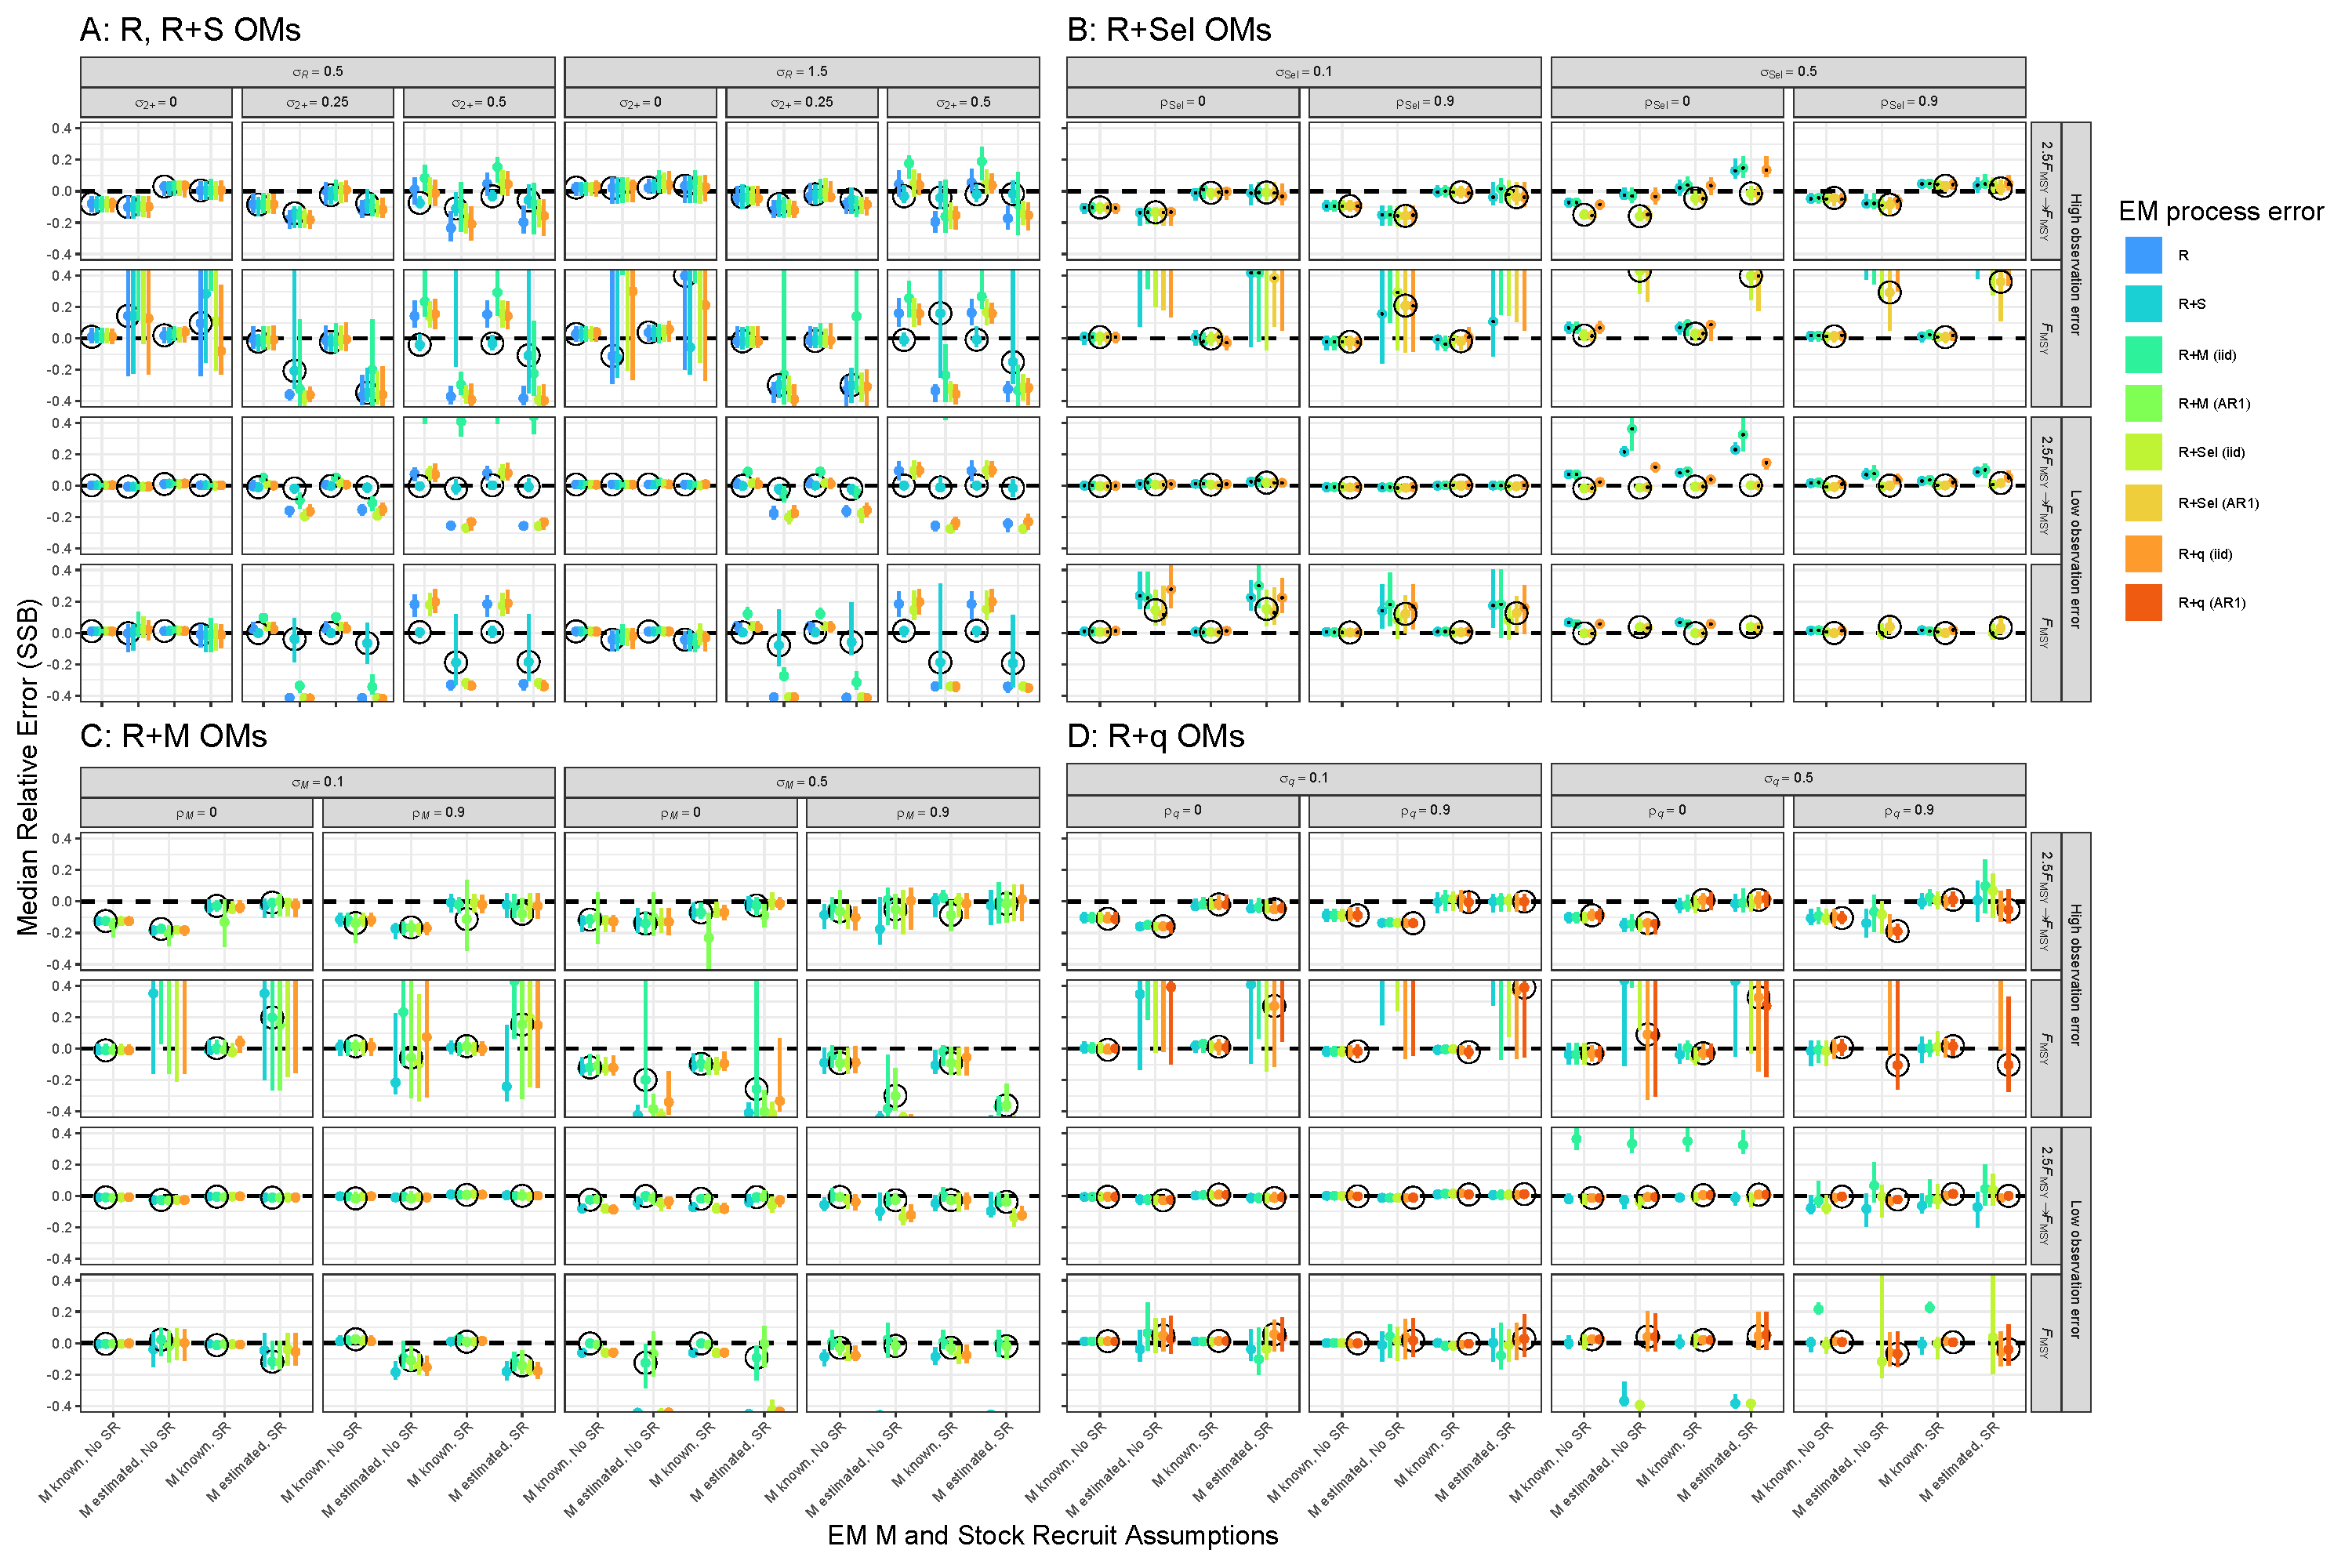
\includegraphics{term_SSB_bias_plots}
%DIFDELCMD < %%%
\DIFdelendFL \DIFaddbeginFL 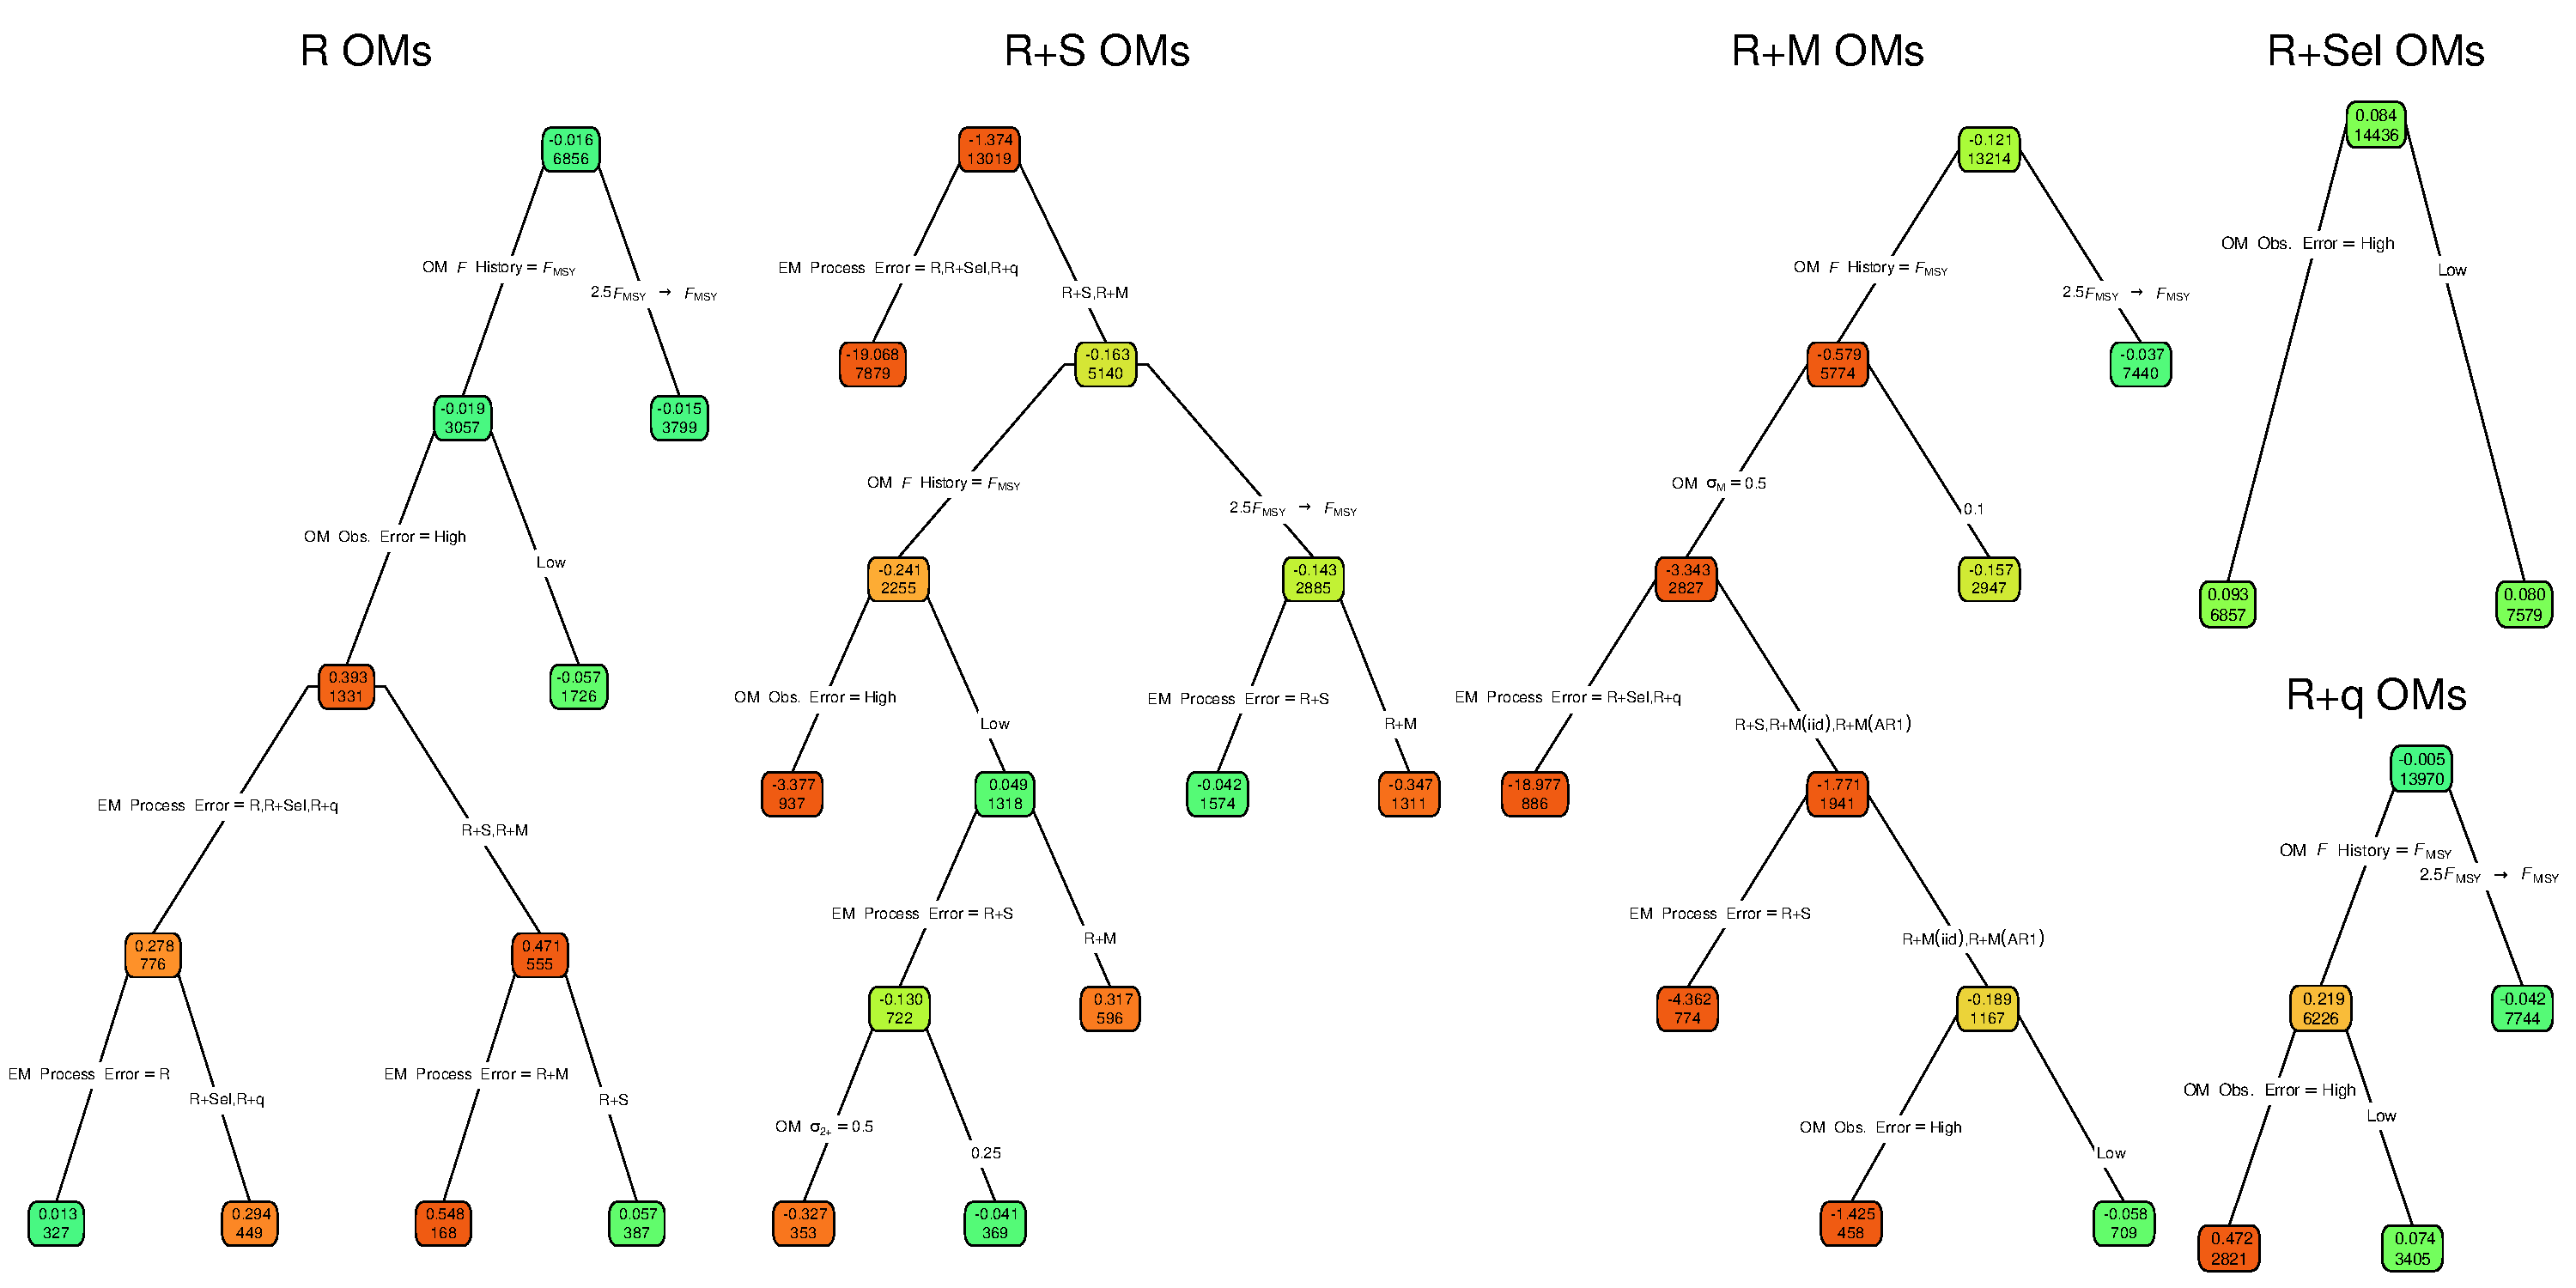
\includegraphics[width = 1.4\textwidth]{med_M_bias_regtree_plots}
\DIFaddendFL \end{center}
\caption{\DIFdelbeginFL \DIFdelFL{Median relative error }\DIFdelendFL \DIFaddbeginFL \DIFaddFL{Regression trees indicating primary factors determining reductions in sums }\DIFaddendFL of \DIFdelbeginFL \DIFdelFL{terminal year SSB }\DIFdelendFL \DIFaddbeginFL \DIFaddFL{squares of errors in estimation measured by Eq. \ref{bias_regression_response} }\DIFaddendFL for \DIFdelbeginFL \DIFdelFL{estimating models fitted to data sets simulated with alternative process error structures: }\DIFdelendFL \DIFaddbeginFL \DIFaddFL{the median natural mortality rate for }\DIFaddendFL R\DIFdelbeginFL \DIFdelFL{and R}\DIFdelendFL +S\DIFdelbeginFL \DIFdelFL{(A)}\DIFdelendFL , R+\DIFdelbeginFL \DIFdelFL{Sel (B)}\DIFdelendFL \DIFaddbeginFL \DIFaddFL{M}\DIFaddendFL , R+\DIFdelbeginFL \DIFdelFL{M (C), or }\DIFdelendFL \DIFaddbeginFL \DIFaddFL{Sel and }\DIFaddendFL R+q \DIFaddbeginFL \DIFaddFL{OMs. Each node shows the median error }\DIFaddendFL (\DIFdelbeginFL \DIFdelFL{D}\DIFdelendFL \DIFaddbeginFL \DIFaddFL{top}\DIFaddendFL ) \DIFaddbeginFL \DIFaddFL{and number of observations (bottom) for the corresponding subset}\DIFaddendFL . \DIFdelbeginFL \DIFdelFL{Circled values indicate results where }\DIFdelendFL \DIFaddbeginFL \DIFaddFL{Lower or higher median absolute errors of }\DIFaddendFL the \DIFdelbeginFL \DIFdelFL{EM }\DIFdelendFL process error \DIFdelbeginFL \DIFdelFL{structure matches that of the operating model and vertical lines represent 95\% confidence intervals}\DIFdelendFL \DIFaddbeginFL \DIFaddFL{assumption are indicated by more green or red polygons, respectively}\DIFaddendFL .}\DIFdelbeginFL %DIFDELCMD < \label{SSB_rel_error}
%DIFDELCMD < %%%
\DIFdelendFL \DIFaddbeginFL \label{med_M_bias_regtree}
\DIFaddendFL \end{figure}
\end{landscape}

\begin{landscape}
\begin{figure}
\begin{center}
\DIFdelbeginFL %DIFDELCMD < 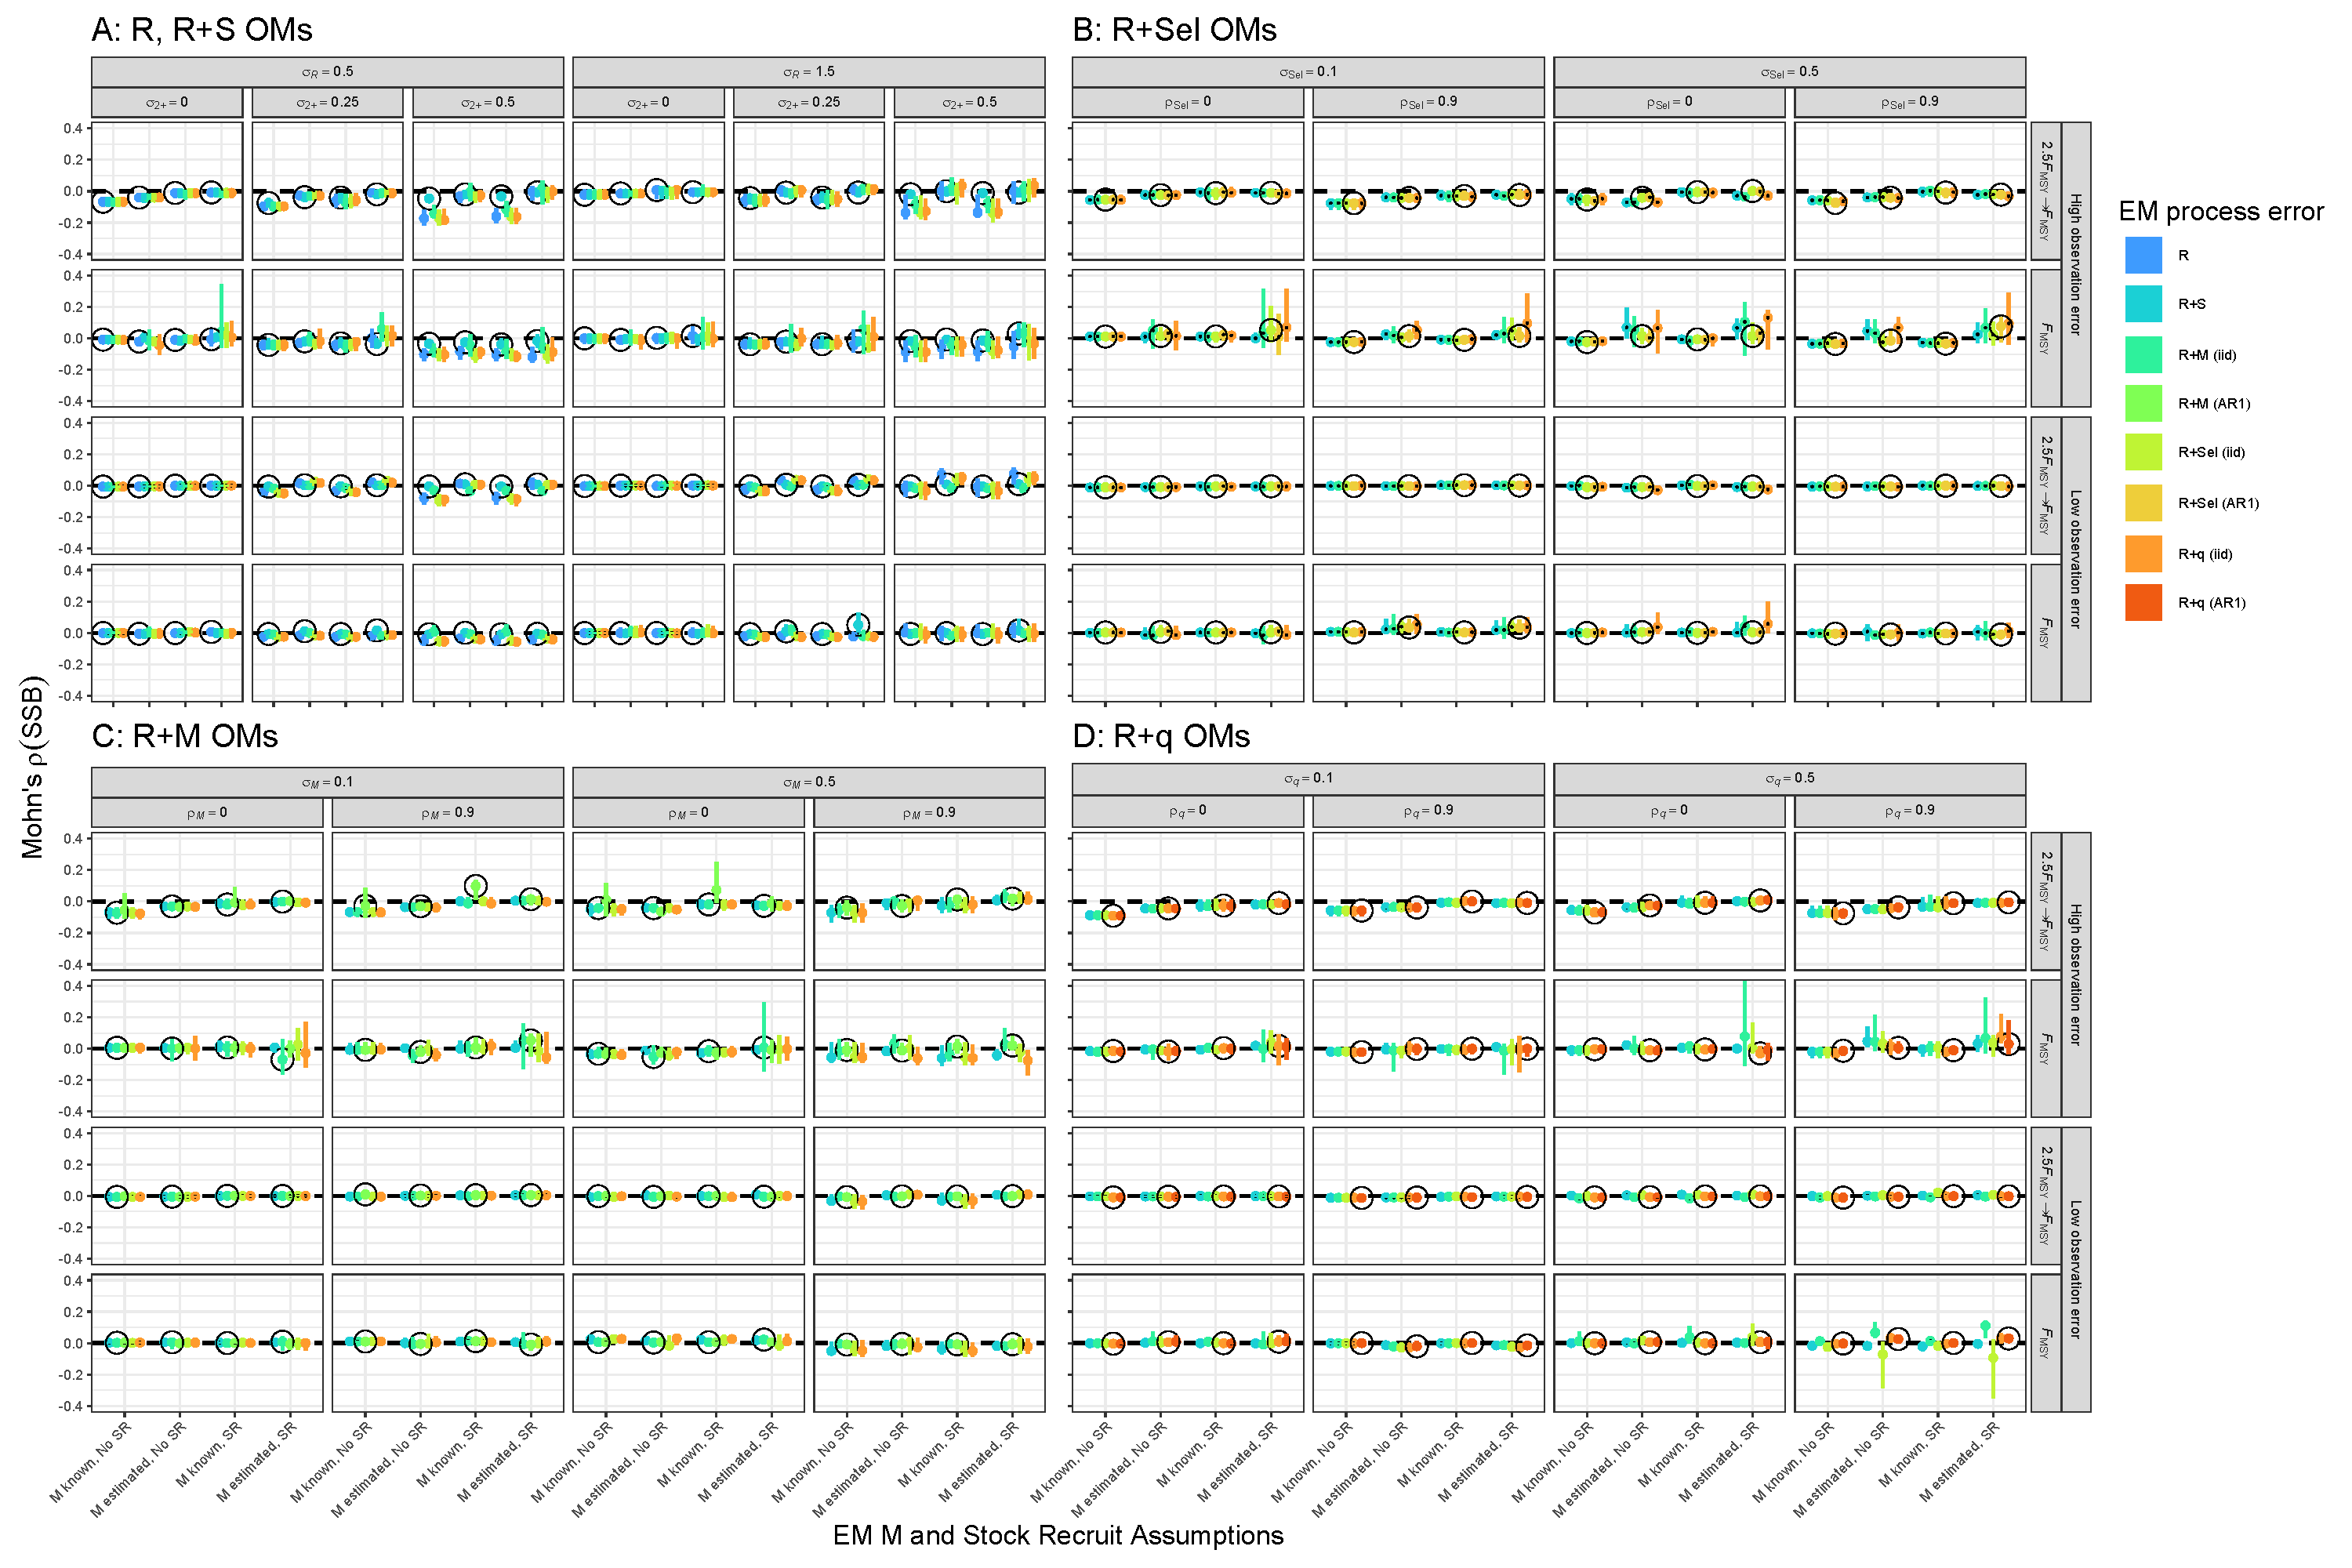
\includegraphics{mohns_rho_ssb_plots}
%DIFDELCMD < %%%
\DIFdelendFL \DIFaddbeginFL 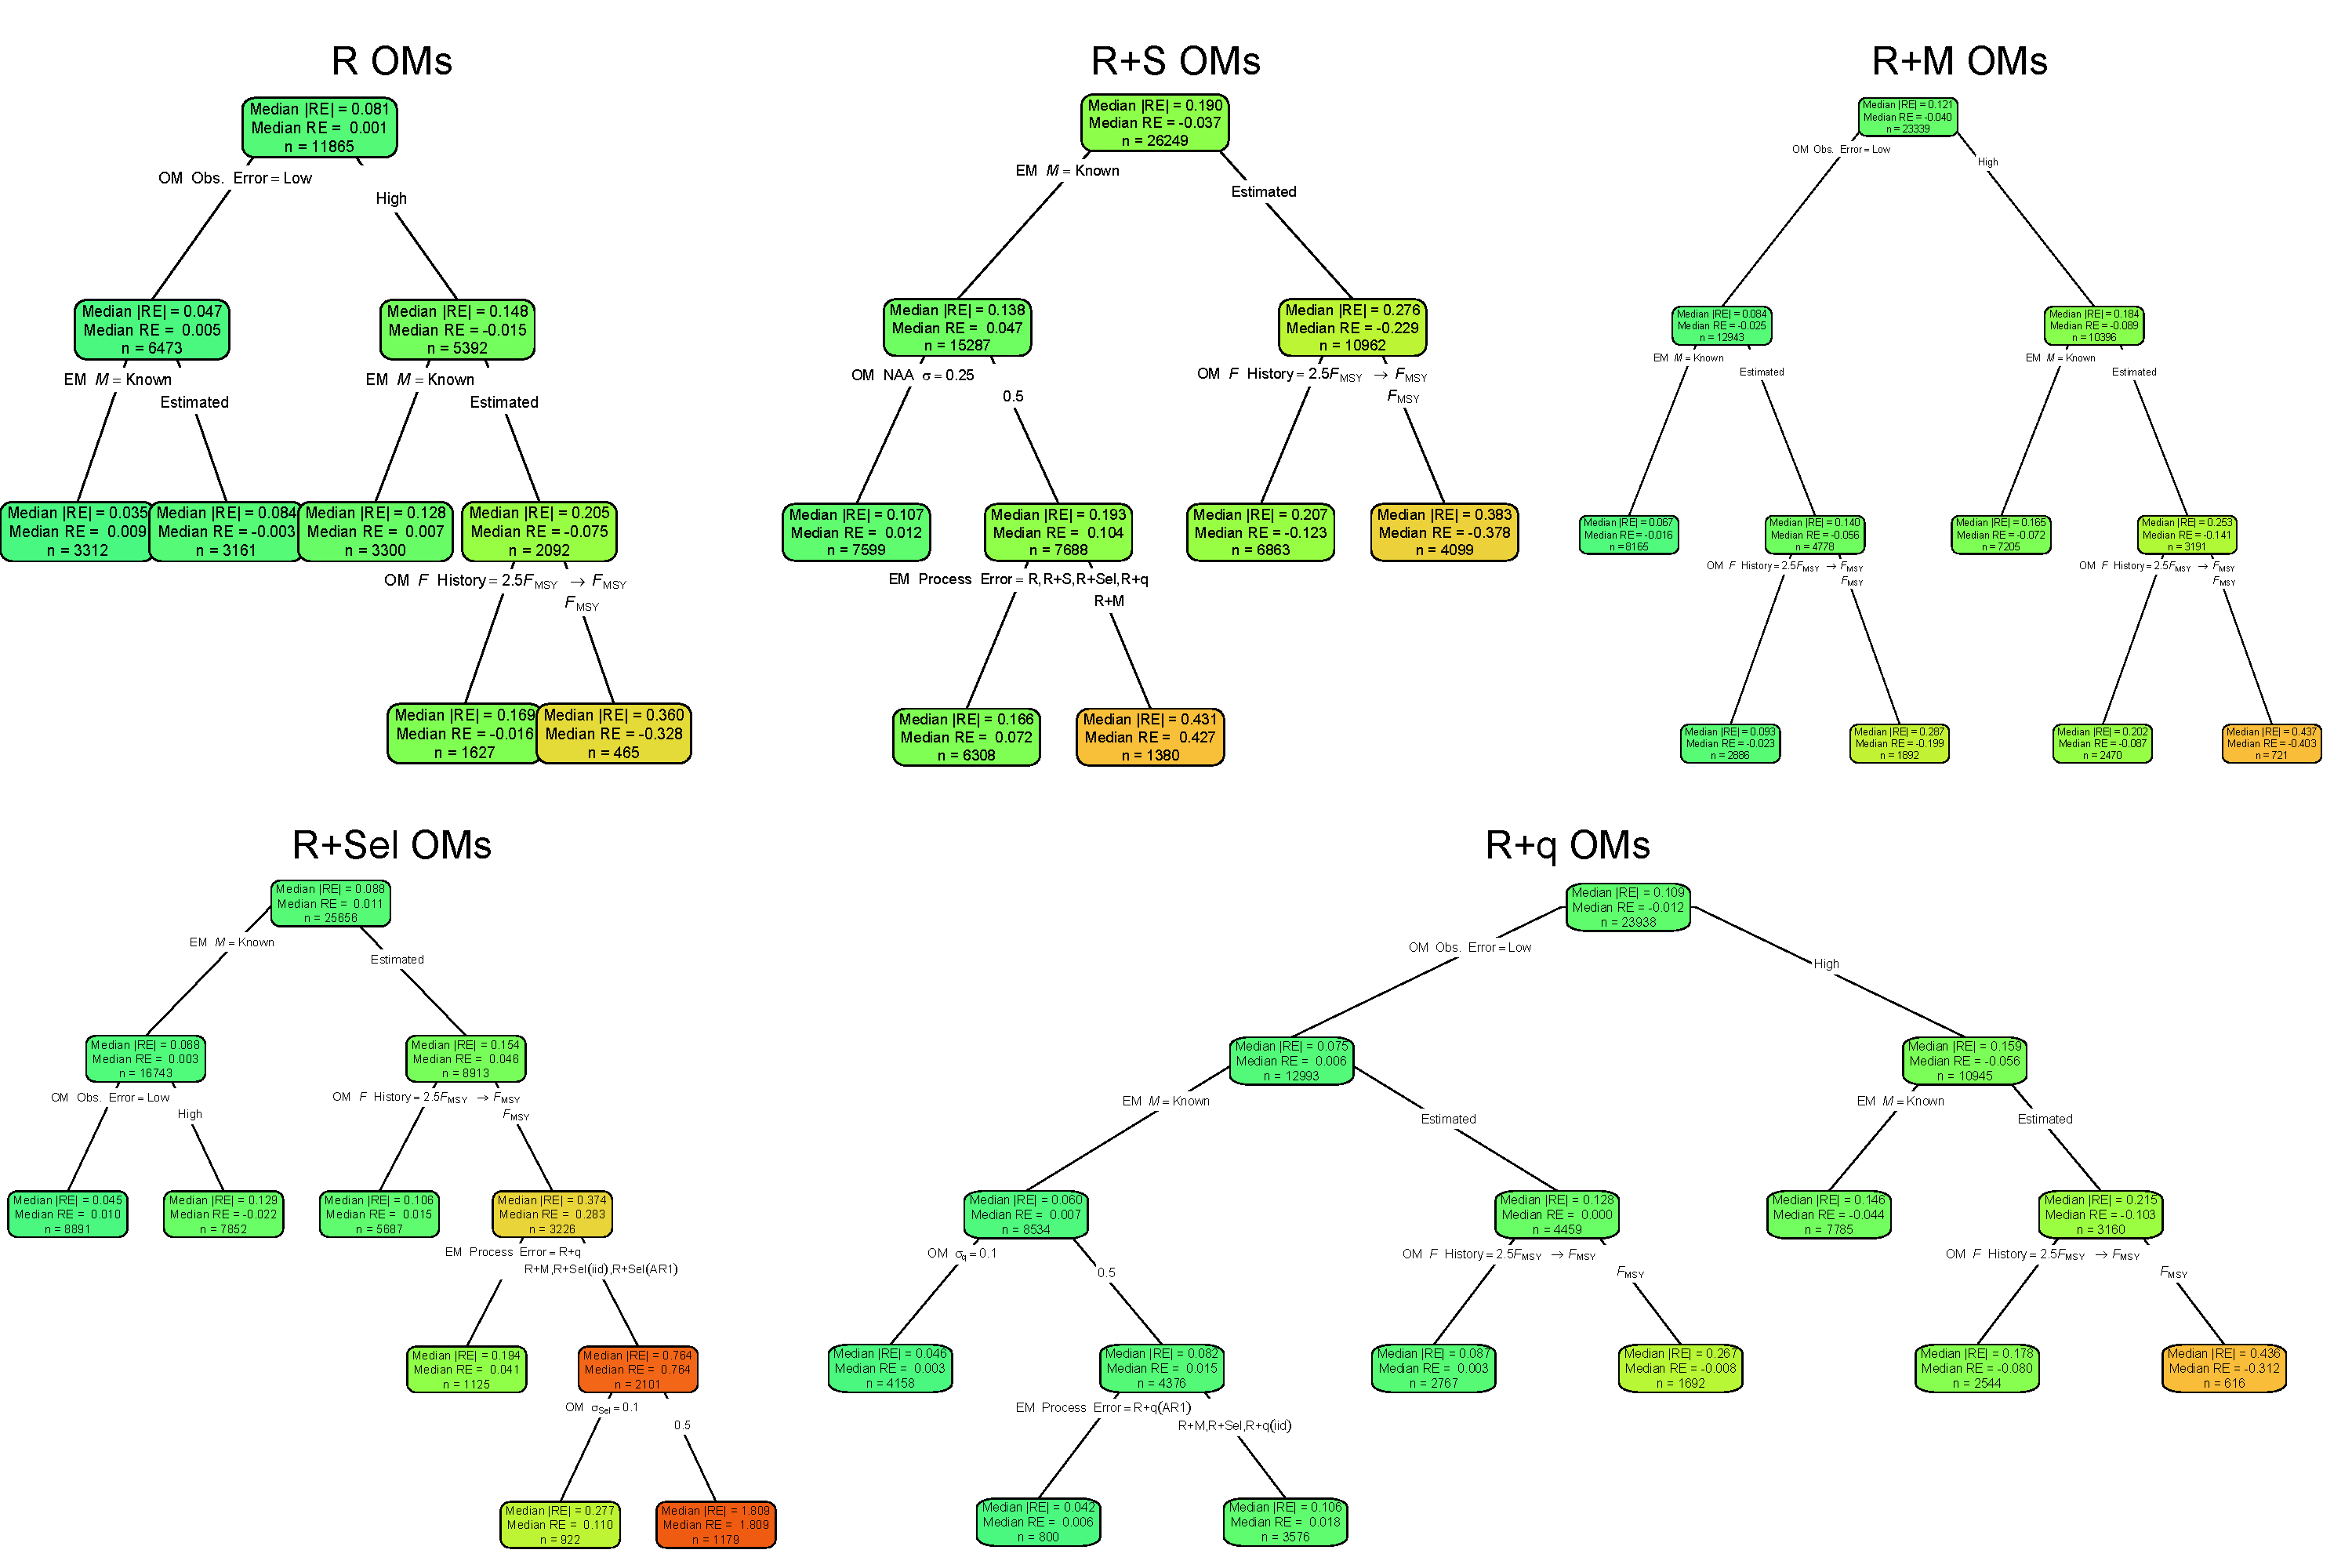
\includegraphics[width = 1.4\textwidth]{SSB_bias_regtree_plots}
\DIFaddendFL \end{center}
\caption{\DIFdelbeginFL \DIFdelFL{Median Mohn's rho }\DIFdelendFL \DIFaddbeginFL \DIFaddFL{Regression trees indicating primary factors determining reductions in sums of squares of errors in estimation measured by Eq. \ref{bias_regression_response} }\DIFaddendFL for \DIFdelbeginFL \DIFdelFL{SSB }\DIFdelendFL \DIFaddbeginFL \DIFaddFL{terminal year spawning stock biomass }\DIFaddendFL for \DIFdelbeginFL \DIFdelFL{estimating models fitted to data sets simulated with alternative process error structures: }\DIFdelendFL R\DIFdelbeginFL \DIFdelFL{and R}\DIFdelendFL +S\DIFdelbeginFL \DIFdelFL{(A)}\DIFdelendFL , R+\DIFdelbeginFL \DIFdelFL{Sel (B)}\DIFdelendFL \DIFaddbeginFL \DIFaddFL{M}\DIFaddendFL , R+\DIFdelbeginFL \DIFdelFL{M (C), or }\DIFdelendFL \DIFaddbeginFL \DIFaddFL{Sel and }\DIFaddendFL R+q \DIFdelbeginFL \DIFdelFL{(D)}\DIFdelendFL \DIFaddbeginFL \DIFaddFL{OMs}\DIFaddendFL . \DIFdelbeginFL \DIFdelFL{Circled values indicate results where }\DIFdelendFL \DIFaddbeginFL \DIFaddFL{Each node shows }\DIFaddendFL the \DIFdelbeginFL \DIFdelFL{EM process }\DIFdelendFL \DIFaddbeginFL \DIFaddFL{median }\DIFaddendFL error \DIFdelbeginFL \DIFdelFL{structure matches that }\DIFdelendFL \DIFaddbeginFL \DIFaddFL{(top) and number }\DIFaddendFL of \DIFaddbeginFL \DIFaddFL{observations (bottom) for }\DIFaddendFL the \DIFdelbeginFL \DIFdelFL{operating model and vertical lines represent 95\% confidence intervals}\DIFdelendFL \DIFaddbeginFL \DIFaddFL{corresponding subset}\DIFaddendFL . \DIFaddbeginFL \DIFaddFL{Median errors closer to or further from zero are indicated by more green or red polygons, respectively.}\DIFaddendFL }\DIFdelbeginFL %DIFDELCMD < \label{mohns_rho_ssb}
%DIFDELCMD < %%%
\DIFdelendFL \DIFaddbeginFL \label{SSB_bias_regtree}
\DIFaddendFL \end{figure}
\end{landscape}

\DIFaddbegin \begin{landscape}
\begin{figure}
\begin{center}
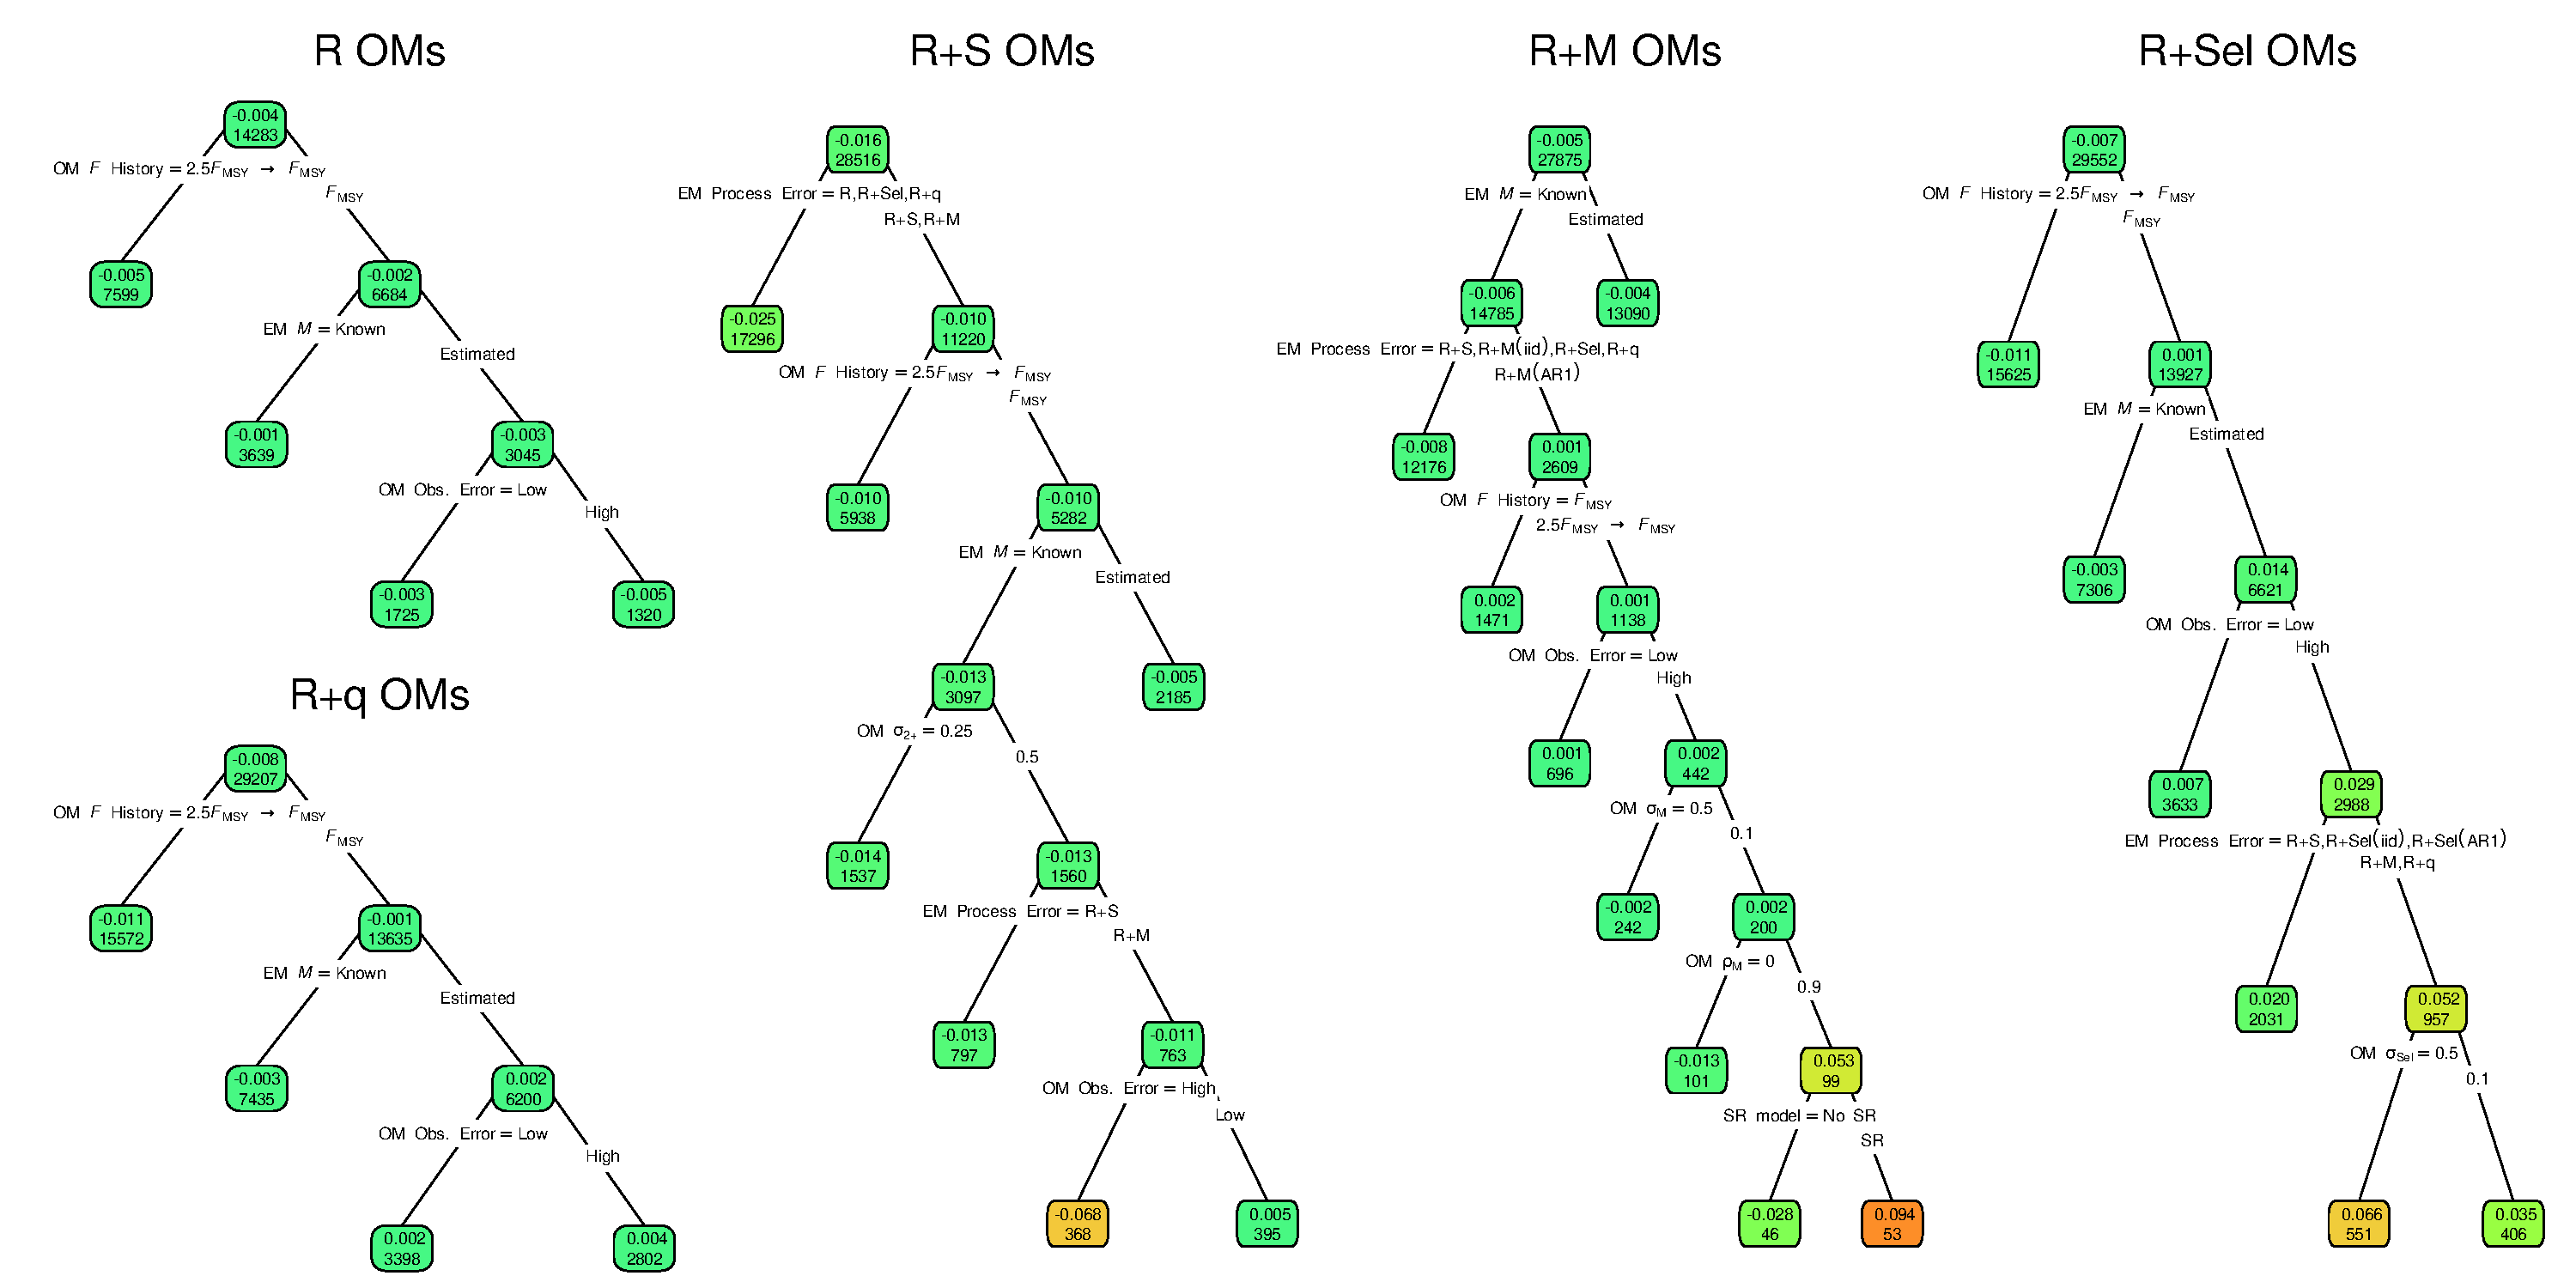
\includegraphics[width = 1.4\textwidth]{SSB_mohns_rho_regtree_plots}
\end{center}
\caption{\DIFaddFL{Regression trees indicating primary factors determining reductions in sums of squares of errors in transformed Mohn's $\rho$ (Eq. \ref{bias_regression_response}) for spawning stock biomass for R+S, R+M, R+Sel and R+q OMs. Each node shows the median Mohn's $\rho$ (top) and number of observations (bottom) for the corresponding subset. Median Mohn's $\rho$ closer to or further from zero are indicated by more green or red polygons, respectively.}}\label{SSB_mohns_rho_regtree}
\end{figure}
\end{landscape}

\DIFaddend \pagebreak

\DIFaddbegin \begin{table}
\caption{\DIFaddFL{For each OM process error type (columns), percent reduction in deviance for logistic regression models fit to indicators of convergence (providing hessian-based standard errors) with each OM and EM factor (rows) included individually, combined, and with second and third order interactions.}}\label{convergence_PRD_table}
{\begin{center}
\begin{tabular}{lrrrrr}
\hline\hline
\multicolumn{1}{l}{\DIFaddFL{Factor}}&\multicolumn{1}{c}{\DIFaddFL{R}}&\multicolumn{1}{c}{\DIFaddFL{R+S}}&\multicolumn{1}{c}{\DIFaddFL{R+M}}&\multicolumn{1}{c}{\DIFaddFL{R+Sel}}&\multicolumn{1}{c}{\DIFaddFL{R+q}}\tabularnewline
\hline
\DIFaddFL{EM Process Error}&\DIFaddFL{27.95}& \DIFaddFL{4.58}&\DIFaddFL{14.68}&\DIFaddFL{17.24}&\DIFaddFL{24.66}\tabularnewline
\DIFaddFL{EM $M$ Assumption}& \DIFaddFL{1.07}&\DIFaddFL{11.43}& \DIFaddFL{2.45}& \DIFaddFL{0.56}& \DIFaddFL{1.46}\tabularnewline
\DIFaddFL{EM SR Assumption}& \DIFaddFL{2.88}& \DIFaddFL{3.30}& \DIFaddFL{1.24}& \DIFaddFL{2.47}& \DIFaddFL{1.59}\tabularnewline
\DIFaddFL{OM Obs. Error}& \DIFaddFL{0.75}& \DIFaddFL{4.64}& \DIFaddFL{2.06}& \DIFaddFL{4.54}& \DIFaddFL{1.60}\tabularnewline
\DIFaddFL{OM $F$ History}& \DIFaddFL{2.32}& \DIFaddFL{3.37}& \DIFaddFL{1.63}& \DIFaddFL{3.30}& \DIFaddFL{2.59}\tabularnewline
\DIFaddFL{OM $\sigma_R$}& \DIFaddFL{0.10}& \DIFaddFL{0.02}&\DIFaddFL{--}&\DIFaddFL{--}&\DIFaddFL{--}\tabularnewline
\DIFaddFL{OM $\sigma_{2+}$ }&\DIFaddFL{--}& \DIFaddFL{0.40}&\DIFaddFL{--}&\DIFaddFL{--}&\DIFaddFL{--}\tabularnewline
\DIFaddFL{OM $\sigma_M$}&\DIFaddFL{--}&\DIFaddFL{--}& \DIFaddFL{0.22}&\DIFaddFL{--}&\DIFaddFL{--}\tabularnewline
\DIFaddFL{OM $\rho_R$}&\DIFaddFL{--}&\DIFaddFL{--}& \DIFaddFL{0.17}&\DIFaddFL{--}&\DIFaddFL{--}\tabularnewline
\DIFaddFL{OM $\sigma_{Sel}$}&\DIFaddFL{--}&\DIFaddFL{--}&\DIFaddFL{--}& \DIFaddFL{1.81}&\DIFaddFL{--}\tabularnewline
\DIFaddFL{OM $\rho_{Sel}$}&\DIFaddFL{--}&\DIFaddFL{--}&\DIFaddFL{--}& \DIFaddFL{0.02}&\DIFaddFL{--}\tabularnewline
\DIFaddFL{OM $\sigma_q$}&\DIFaddFL{--}&\DIFaddFL{--}&\DIFaddFL{--}&\DIFaddFL{--}& \DIFaddFL{0.34}\tabularnewline
\DIFaddFL{OM $\rho_q$}&\DIFaddFL{--}&\DIFaddFL{--}&\DIFaddFL{--}&\DIFaddFL{--}&\DIFaddFL{\textless  0.01}\tabularnewline
\DIFaddFL{All factors}&\DIFaddFL{39.54}&\DIFaddFL{31.46}&\DIFaddFL{24.85}&\DIFaddFL{34.83}&\DIFaddFL{36.31}\tabularnewline
\DIFaddFL{+ All Two Way}&\DIFaddFL{45.03}&\DIFaddFL{39.89}&\DIFaddFL{35.20}&\DIFaddFL{42.81}&\DIFaddFL{43.70}\tabularnewline
\DIFaddFL{+ All Three Way}&\DIFaddFL{47.02}&\DIFaddFL{44.57}&\DIFaddFL{37.88}&\DIFaddFL{45.51}&\DIFaddFL{46.87}\tabularnewline
\hline
\end{tabular}\end{center}
}
\end{table}

\begin{table}
\caption{\DIFaddFL{For each OM process error type (columns), percent reduction in deviance for multinomial logistic regression models fit to indicators of EM process error assumption with lowest AIC with each OM and EM factor (rows) included individually, combined, and with second and third order interactions.}}\label{AIC_PE_PRD_table}
{\begin{center}
\begin{tabular}{lrrrrr}
\hline\hline
\multicolumn{1}{l}{\DIFaddFL{Factor}}&\multicolumn{1}{c}{\DIFaddFL{R}}&\multicolumn{1}{c}{\DIFaddFL{R+S}}&\multicolumn{1}{c}{\DIFaddFL{R+M}}&\multicolumn{1}{c}{\DIFaddFL{R+Sel}}&\multicolumn{1}{c}{\DIFaddFL{R+q}}\tabularnewline
\hline
\DIFaddFL{EM $M$ Assumption}& \DIFaddFL{5.52}& \DIFaddFL{1.05}& \DIFaddFL{0.52}& \DIFaddFL{0.61}& \DIFaddFL{1.32}\tabularnewline
\DIFaddFL{EM SR Assumption}& \DIFaddFL{5.60}& \DIFaddFL{0.75}& \DIFaddFL{1.13}& \DIFaddFL{0.93}& \DIFaddFL{1.95}\tabularnewline
\DIFaddFL{OM Obs. Error}& \DIFaddFL{2.96}&\DIFaddFL{22.46}& \DIFaddFL{3.42}&\DIFaddFL{25.67}& \DIFaddFL{5.03}\tabularnewline
\DIFaddFL{OM $F$ History}& \DIFaddFL{5.77}& \DIFaddFL{0.62}& \DIFaddFL{0.94}& \DIFaddFL{0.91}& \DIFaddFL{2.05}\tabularnewline
\DIFaddFL{OM $\sigma_R$}& \DIFaddFL{0.10}& \DIFaddFL{0.66}&\DIFaddFL{--}&\DIFaddFL{--}&\DIFaddFL{--}\tabularnewline
\DIFaddFL{OM $\sigma_{2+}$ }&\DIFaddFL{--}&\DIFaddFL{16.86}&\DIFaddFL{--}&\DIFaddFL{--}&\DIFaddFL{--}\tabularnewline
\DIFaddFL{OM $\sigma_M$}&\DIFaddFL{--}&\DIFaddFL{--}& \DIFaddFL{9.06}&\DIFaddFL{--}&\DIFaddFL{--}\tabularnewline
\DIFaddFL{OM $\rho_R$}&\DIFaddFL{--}&\DIFaddFL{--}& \DIFaddFL{0.38}&\DIFaddFL{--}&\DIFaddFL{--}\tabularnewline
\DIFaddFL{OM $\sigma_{Sel}$}&\DIFaddFL{--}&\DIFaddFL{--}&\DIFaddFL{--}& \DIFaddFL{7.59}&\DIFaddFL{--}\tabularnewline
\DIFaddFL{OM $\rho_{Sel}$}&\DIFaddFL{--}&\DIFaddFL{--}&\DIFaddFL{--}& \DIFaddFL{0.60}&\DIFaddFL{--}\tabularnewline
\DIFaddFL{OM $\sigma_q$}&\DIFaddFL{--}&\DIFaddFL{--}&\DIFaddFL{--}&\DIFaddFL{--}&\DIFaddFL{13.50}\tabularnewline
\DIFaddFL{OM $\rho_q$}&\DIFaddFL{--}&\DIFaddFL{--}&\DIFaddFL{--}&\DIFaddFL{--}& \DIFaddFL{0.75}\tabularnewline
\DIFaddFL{All factors}&\DIFaddFL{20.98}&\DIFaddFL{46.12}&\DIFaddFL{16.58}&\DIFaddFL{40.83}&\DIFaddFL{25.99}\tabularnewline
\DIFaddFL{+ All Two Way}&\DIFaddFL{22.02}&\DIFaddFL{48.94}&\DIFaddFL{21.63}&\DIFaddFL{44.08}&\DIFaddFL{30.17}\tabularnewline
\DIFaddFL{+ All Three Way}&\DIFaddFL{22.05}&\DIFaddFL{49.98}&\DIFaddFL{22.36}&\DIFaddFL{44.54}&\DIFaddFL{31.38}\tabularnewline
\hline
\end{tabular}\end{center}
}
\end{table}

\begin{table}
\caption{\DIFaddFL{For each OM process error type (columns), percent reduction in deviance for logistic regression models fit to indicators of EM stock-recruit assumption (none or Beverton-Holt) with lowest AIC with each OM and EM factor (rows) included individually, combined, and with second and third order interactions.}}\label{AIC_SRR_PRD_table}
{\begin{center}
\begin{tabular}{lrrrrr}
\hline\hline
\multicolumn{1}{l}{\DIFaddFL{Factor}}&\multicolumn{1}{c}{\DIFaddFL{R}}&\multicolumn{1}{c}{\DIFaddFL{R+S}}&\multicolumn{1}{c}{\DIFaddFL{R+M}}&\multicolumn{1}{c}{\DIFaddFL{R+Sel}}&\multicolumn{1}{c}{\DIFaddFL{R+q}}\tabularnewline
\hline
\DIFaddFL{EM $M$ Assumption}& \DIFaddFL{0.04}& \DIFaddFL{0.21}& \DIFaddFL{0.18}& \DIFaddFL{0.02}& \DIFaddFL{0.01}\tabularnewline
\DIFaddFL{OM Obs. Error}&\DIFaddFL{\textless  0.01}& \DIFaddFL{0.65}& \DIFaddFL{0.14}& \DIFaddFL{0.04}& \DIFaddFL{0.02}\tabularnewline
\DIFaddFL{OM $F$ History}& \DIFaddFL{9.17}& \DIFaddFL{3.79}&\DIFaddFL{13.08}&\DIFaddFL{26.56}&\DIFaddFL{24.60}\tabularnewline
\DIFaddFL{OM $\sigma_R$}& \DIFaddFL{3.54}& \DIFaddFL{4.74}&\DIFaddFL{--}&\DIFaddFL{--}&\DIFaddFL{--}\tabularnewline
\DIFaddFL{OM $\sigma_{2+}$ }&\DIFaddFL{--}& \DIFaddFL{0.14}&\DIFaddFL{--}&\DIFaddFL{--}&\DIFaddFL{--}\tabularnewline
\DIFaddFL{OM $\sigma_M$}&\DIFaddFL{--}&\DIFaddFL{--}& \DIFaddFL{1.14}&\DIFaddFL{--}&\DIFaddFL{--}\tabularnewline
\DIFaddFL{OM $\rho_R$}&\DIFaddFL{--}&\DIFaddFL{--}& \DIFaddFL{0.05}&\DIFaddFL{--}&\DIFaddFL{--}\tabularnewline
\DIFaddFL{OM $\sigma_{Sel}$}&\DIFaddFL{--}&\DIFaddFL{--}&\DIFaddFL{--}& \DIFaddFL{0.02}&\DIFaddFL{--}\tabularnewline
\DIFaddFL{OM $\rho_{Sel}$}&\DIFaddFL{--}&\DIFaddFL{--}&\DIFaddFL{--}& \DIFaddFL{0.17}&\DIFaddFL{--}\tabularnewline
\DIFaddFL{OM $\sigma_q$}&\DIFaddFL{--}&\DIFaddFL{--}&\DIFaddFL{--}&\DIFaddFL{--}& \DIFaddFL{0.36}\tabularnewline
\DIFaddFL{OM $\rho_q$}&\DIFaddFL{--}&\DIFaddFL{--}&\DIFaddFL{--}&\DIFaddFL{--}& \DIFaddFL{0.02}\tabularnewline
\DIFaddFL{$\log\left(\text{SD}_\text{SSB}\right)$}& \DIFaddFL{4.11}& \DIFaddFL{1.59}&\DIFaddFL{33.39}&\DIFaddFL{41.36}&\DIFaddFL{39.23}\tabularnewline
\DIFaddFL{All factors}&\DIFaddFL{31.52}&\DIFaddFL{18.99}&\DIFaddFL{34.23}&\DIFaddFL{43.77}&\DIFaddFL{42.31}\tabularnewline
\DIFaddFL{+ All Two Way}&\DIFaddFL{34.79}&\DIFaddFL{22.24}&\DIFaddFL{35.99}&\DIFaddFL{45.84}&\DIFaddFL{44.04}\tabularnewline
\DIFaddFL{+ All Three Way}&\DIFaddFL{35.41}&\DIFaddFL{23.09}&\DIFaddFL{37.57}&\DIFaddFL{46.39}&\DIFaddFL{44.63}\tabularnewline
\hline
\end{tabular}\end{center}
}
\end{table}

\begin{landscape}
\begin{table}
\caption{\DIFaddFL{For each OM process error type (columns), percent reduction in deviance for linear regression models fit to errors in estimation measured by Eq. \ref{bias_regression_response} for the Beverton-Holt stock recruit relation ship parameters with each OM and EM factor (rows) included individually, combined, and with second and third order interactions.}}\label{bias_SR_pars_PRD_table}
{\begin{center}
\begin{tabular}{lrrrrrcrrrrr}
\hline\hline
\multicolumn{1}{l}{\bfseries \DIFaddFL{Factor}}&\multicolumn{5}{c}{\bfseries \DIFaddFL{Beverton-Holt $a$}}&\multicolumn{1}{c}{\bfseries }&\multicolumn{5}{c}{\bfseries \DIFaddFL{Beverton-Holt $b$}}\tabularnewline
\cline{2-6} \cline{8-12}
\multicolumn{1}{l}{}&\multicolumn{1}{c}{\DIFaddFL{R}}&\multicolumn{1}{c}{\DIFaddFL{R+S}}&\multicolumn{1}{c}{\DIFaddFL{R+M}}&\multicolumn{1}{c}{\DIFaddFL{R+Sel}}&\multicolumn{1}{c}{\DIFaddFL{R+q}}&\multicolumn{1}{c}{}&\multicolumn{1}{c}{\DIFaddFL{R}}&\multicolumn{1}{c}{\DIFaddFL{R+S}}&\multicolumn{1}{c}{\DIFaddFL{R+M}}&\multicolumn{1}{c}{\DIFaddFL{R+Sel}}&\multicolumn{1}{c}{\DIFaddFL{R+q}}\tabularnewline
\hline
\DIFaddFL{EM $M$ Assumption}& \DIFaddFL{0.02}& \DIFaddFL{1.05}& \DIFaddFL{0.02}& \DIFaddFL{0.11}& \DIFaddFL{0.02}&& \DIFaddFL{0.05}& \DIFaddFL{1.06}& \DIFaddFL{0.03}& \DIFaddFL{0.01}& \DIFaddFL{0.40}\tabularnewline
\DIFaddFL{EM Process Error}& \DIFaddFL{2.74}& \DIFaddFL{0.18}& \DIFaddFL{0.20}& \DIFaddFL{1.25}& \DIFaddFL{1.90}&& \DIFaddFL{2.29}& \DIFaddFL{1.21}& \DIFaddFL{0.12}& \DIFaddFL{1.40}& \DIFaddFL{3.06}\tabularnewline
\DIFaddFL{OM Obs. Error}& \DIFaddFL{0.16}&\DIFaddFL{\textless  0.01}& \DIFaddFL{0.01}& \DIFaddFL{0.04}&\DIFaddFL{\textless  0.01}&&\DIFaddFL{\textless  0.01}& \DIFaddFL{0.01}& \DIFaddFL{0.05}& \DIFaddFL{0.01}& \DIFaddFL{0.01}\tabularnewline
\DIFaddFL{OM $F$ History}& \DIFaddFL{3.15}& \DIFaddFL{3.34}& \DIFaddFL{5.60}&\DIFaddFL{11.37}&\DIFaddFL{10.00}&& \DIFaddFL{1.16}& \DIFaddFL{1.17}& \DIFaddFL{2.01}& \DIFaddFL{7.97}& \DIFaddFL{3.87}\tabularnewline
\DIFaddFL{OM $\sigma_R$}& \DIFaddFL{2.31}& \DIFaddFL{0.74}&\DIFaddFL{--}&\DIFaddFL{--}&\DIFaddFL{--}&& \DIFaddFL{1.67}& \DIFaddFL{0.52}&\DIFaddFL{--}&\DIFaddFL{--}&\DIFaddFL{--}\tabularnewline
\DIFaddFL{OM $\sigma_{2+}$ }&\DIFaddFL{--}& \DIFaddFL{0.29}&\DIFaddFL{--}&\DIFaddFL{--}&\DIFaddFL{--}&&\DIFaddFL{--}& \DIFaddFL{0.01}&\DIFaddFL{--}&\DIFaddFL{--}&\DIFaddFL{--}\tabularnewline
\DIFaddFL{OM $\sigma_M$}&\DIFaddFL{--}&\DIFaddFL{--}& \DIFaddFL{0.30}&\DIFaddFL{--}&\DIFaddFL{--}&&\DIFaddFL{--}&\DIFaddFL{--}& \DIFaddFL{0.13}&\DIFaddFL{--}&\DIFaddFL{--}\tabularnewline
\DIFaddFL{OM $\rho_R$}&\DIFaddFL{--}&\DIFaddFL{--}& \DIFaddFL{0.51}&\DIFaddFL{--}&\DIFaddFL{--}&&\DIFaddFL{--}&\DIFaddFL{--}& \DIFaddFL{0.22}&\DIFaddFL{--}&\DIFaddFL{--}\tabularnewline
\DIFaddFL{OM $\sigma_{Sel}$}&\DIFaddFL{--}&\DIFaddFL{--}&\DIFaddFL{--}& \DIFaddFL{0.13}&\DIFaddFL{--}&&\DIFaddFL{--}&\DIFaddFL{--}&\DIFaddFL{--}& \DIFaddFL{0.05}&\DIFaddFL{--}\tabularnewline
\DIFaddFL{OM $\rho_{Sel}$}&\DIFaddFL{--}&\DIFaddFL{--}&\DIFaddFL{--}& \DIFaddFL{0.07}&\DIFaddFL{--}&&\DIFaddFL{--}&\DIFaddFL{--}&\DIFaddFL{--}& \DIFaddFL{0.04}&\DIFaddFL{--}\tabularnewline
\DIFaddFL{OM $\sigma_q$}&\DIFaddFL{--}&\DIFaddFL{--}&\DIFaddFL{--}&\DIFaddFL{--}& \DIFaddFL{0.04}&&\DIFaddFL{--}&\DIFaddFL{--}&\DIFaddFL{--}&\DIFaddFL{--}& \DIFaddFL{0.10}\tabularnewline
\DIFaddFL{OM $\rho_q$}&\DIFaddFL{--}&\DIFaddFL{--}&\DIFaddFL{--}&\DIFaddFL{--}&\DIFaddFL{\textless  0.01}&&\DIFaddFL{--}&\DIFaddFL{--}&\DIFaddFL{--}&\DIFaddFL{--}&\DIFaddFL{\textless  0.01}\tabularnewline
\DIFaddFL{All factors}& \DIFaddFL{8.07}& \DIFaddFL{5.15}& \DIFaddFL{6.73}&\DIFaddFL{12.64}&\DIFaddFL{11.79}&& \DIFaddFL{4.91}& \DIFaddFL{3.75}& \DIFaddFL{2.55}& \DIFaddFL{9.12}& \DIFaddFL{7.22}\tabularnewline
\DIFaddFL{+ All Two Way}& \DIFaddFL{9.96}& \DIFaddFL{7.37}& \DIFaddFL{9.76}&\DIFaddFL{13.59}&\DIFaddFL{13.65}&& \DIFaddFL{7.55}& \DIFaddFL{7.15}& \DIFaddFL{4.32}&\DIFaddFL{10.08}&\DIFaddFL{12.16}\tabularnewline
\DIFaddFL{+ All Three Way}&\DIFaddFL{11.22}& \DIFaddFL{8.15}&\DIFaddFL{11.13}&\DIFaddFL{14.48}&\DIFaddFL{14.87}&& \DIFaddFL{9.78}& \DIFaddFL{9.02}& \DIFaddFL{5.26}&\DIFaddFL{11.08}&\DIFaddFL{14.73}\tabularnewline
\hline
\end{tabular}\end{center}
}
\end{table}
\end{landscape}

\begin{table}
\caption{\DIFaddFL{For each OM process error type (columns), percent reduction in deviance for linear regression models fit to errors in estimation measured by Eq. \ref{bias_regression_response} for the median natural mortality rate parameter with each OM and EM factor (rows) included individually, combined, and with second and third order interactions.}}\label{bias_median_M_PRD_table}
{\begin{center}
\begin{tabular}{lrrrrr}
\hline\hline
\multicolumn{1}{l}{\DIFaddFL{Factor}}&\multicolumn{1}{c}{\DIFaddFL{R}}&\multicolumn{1}{c}{\DIFaddFL{R+S}}&\multicolumn{1}{c}{\DIFaddFL{R+M}}&\multicolumn{1}{c}{\DIFaddFL{R+Sel}}&\multicolumn{1}{c}{\DIFaddFL{R+q}}\tabularnewline
\hline
\DIFaddFL{EM SR assumption}& \DIFaddFL{0.21}& \DIFaddFL{0.38}& \DIFaddFL{0.11}& \DIFaddFL{0.26}& \DIFaddFL{0.43}\tabularnewline
\DIFaddFL{EM Process Error}& \DIFaddFL{1.98}&\DIFaddFL{20.36}& \DIFaddFL{3.16}& \DIFaddFL{0.94}& \DIFaddFL{1.31}\tabularnewline
\DIFaddFL{OM Obs. Error}& \DIFaddFL{4.74}& \DIFaddFL{0.79}& \DIFaddFL{0.40}& \DIFaddFL{2.23}& \DIFaddFL{1.88}\tabularnewline
\DIFaddFL{OM $F$ History}& \DIFaddFL{5.07}&\DIFaddFL{15.11}&\DIFaddFL{10.65}& \DIFaddFL{0.24}& \DIFaddFL{2.38}\tabularnewline
\DIFaddFL{OM $\sigma_R$}&\DIFaddFL{\textless  0.01}& \DIFaddFL{0.01}&\DIFaddFL{--}&\DIFaddFL{--}&\DIFaddFL{--}\tabularnewline
\DIFaddFL{OM $\sigma_{2+}$ }&\DIFaddFL{--}& \DIFaddFL{5.04}&\DIFaddFL{--}&\DIFaddFL{--}&\DIFaddFL{--}\tabularnewline
\DIFaddFL{OM $\sigma_M$}&\DIFaddFL{--}&\DIFaddFL{--}& \DIFaddFL{5.32}&\DIFaddFL{--}&\DIFaddFL{--}\tabularnewline
\DIFaddFL{OM $\rho_R$}&\DIFaddFL{--}&\DIFaddFL{--}& \DIFaddFL{0.85}&\DIFaddFL{--}&\DIFaddFL{--}\tabularnewline
\DIFaddFL{OM $\sigma_{Sel}$}&\DIFaddFL{--}&\DIFaddFL{--}&\DIFaddFL{--}& \DIFaddFL{1.30}&\DIFaddFL{--}\tabularnewline
\DIFaddFL{OM $\rho_{Sel}$}&\DIFaddFL{--}&\DIFaddFL{--}&\DIFaddFL{--}& \DIFaddFL{0.37}&\DIFaddFL{--}\tabularnewline
\DIFaddFL{OM $\sigma_q$}&\DIFaddFL{--}&\DIFaddFL{--}&\DIFaddFL{--}&\DIFaddFL{--}& \DIFaddFL{0.46}\tabularnewline
\DIFaddFL{OM $\rho_q$}&\DIFaddFL{--}&\DIFaddFL{--}&\DIFaddFL{--}&\DIFaddFL{--}& \DIFaddFL{0.06}\tabularnewline
\DIFaddFL{All factors}&\DIFaddFL{12.64}&\DIFaddFL{40.10}&\DIFaddFL{21.29}& \DIFaddFL{5.54}& \DIFaddFL{6.52}\tabularnewline
\DIFaddFL{+ All Two Way}&\DIFaddFL{21.17}&\DIFaddFL{48.12}&\DIFaddFL{36.19}& \DIFaddFL{9.87}&\DIFaddFL{11.71}\tabularnewline
\DIFaddFL{+ All Three Way}&\DIFaddFL{23.03}&\DIFaddFL{50.38}&\DIFaddFL{42.82}&\DIFaddFL{11.58}&\DIFaddFL{14.64}\tabularnewline
\hline
\end{tabular}\end{center}
}
\end{table}

\begin{table}
\caption{\DIFaddFL{For each OM process error type (columns), percent reduction in deviance for linear regression models fit to errors in estimation measured by Eq. \ref{bias_regression_response} for the terminal year spawning biomass with each OM and EM factor (rows) included individually, combined, and with second and third order interactions.}}\label{bias_SSB_PRD_table}
{\begin{center}
\begin{tabular}{lrrrrr}
\hline\hline
\multicolumn{1}{l}{\DIFaddFL{Factor}}&\multicolumn{1}{c}{\DIFaddFL{R}}&\multicolumn{1}{c}{\DIFaddFL{R+S}}&\multicolumn{1}{c}{\DIFaddFL{R+M}}&\multicolumn{1}{c}{\DIFaddFL{R+Sel}}&\multicolumn{1}{c}{\DIFaddFL{R+q}}\tabularnewline
\hline
\DIFaddFL{EM $M$ Assumption}& \DIFaddFL{2.28}& \DIFaddFL{1.15}& \DIFaddFL{1.04}& \DIFaddFL{2.92}& \DIFaddFL{3.26}\tabularnewline
\DIFaddFL{EM SR assumption}& \DIFaddFL{0.10}& \DIFaddFL{0.06}& \DIFaddFL{0.08}& \DIFaddFL{0.06}& \DIFaddFL{0.08}\tabularnewline
\DIFaddFL{EM Process Error}& \DIFaddFL{0.43}& \DIFaddFL{4.28}& \DIFaddFL{0.40}& \DIFaddFL{0.11}& \DIFaddFL{1.05}\tabularnewline
\DIFaddFL{OM Obs. Error}& \DIFaddFL{1.63}& \DIFaddFL{0.07}& \DIFaddFL{0.78}& \DIFaddFL{0.32}&\DIFaddFL{\textless  0.01}\tabularnewline
\DIFaddFL{OM $F$ History}& \DIFaddFL{2.62}& \DIFaddFL{3.15}& \DIFaddFL{1.28}& \DIFaddFL{3.22}& \DIFaddFL{4.72}\tabularnewline
\DIFaddFL{OM $\sigma_R$}& \DIFaddFL{0.03}& \DIFaddFL{0.01}&\DIFaddFL{--}&\DIFaddFL{--}&\DIFaddFL{--}\tabularnewline
\DIFaddFL{OM $\sigma_{2+}$ }&\DIFaddFL{--}& \DIFaddFL{0.93}&\DIFaddFL{--}&\DIFaddFL{--}&\DIFaddFL{--}\tabularnewline
\DIFaddFL{OM $\sigma_M$}&\DIFaddFL{--}&\DIFaddFL{--}& \DIFaddFL{0.18}&\DIFaddFL{--}&\DIFaddFL{--}\tabularnewline
\DIFaddFL{OM $\rho_R$}&\DIFaddFL{--}&\DIFaddFL{--}& \DIFaddFL{0.01}&\DIFaddFL{--}&\DIFaddFL{--}\tabularnewline
\DIFaddFL{OM $\sigma_{Sel}$}&\DIFaddFL{--}&\DIFaddFL{--}&\DIFaddFL{--}& \DIFaddFL{0.16}&\DIFaddFL{--}\tabularnewline
\DIFaddFL{OM $\rho_{Sel}$}&\DIFaddFL{--}&\DIFaddFL{--}&\DIFaddFL{--}& \DIFaddFL{0.04}&\DIFaddFL{--}\tabularnewline
\DIFaddFL{OM $\sigma_q$}&\DIFaddFL{--}&\DIFaddFL{--}&\DIFaddFL{--}&\DIFaddFL{--}& \DIFaddFL{1.02}\tabularnewline
\DIFaddFL{OM $\rho_q$}&\DIFaddFL{--}&\DIFaddFL{--}&\DIFaddFL{--}&\DIFaddFL{--}& \DIFaddFL{0.06}\tabularnewline
\DIFaddFL{All factors}& \DIFaddFL{7.59}& \DIFaddFL{9.86}& \DIFaddFL{3.93}& \DIFaddFL{7.04}&\DIFaddFL{10.64}\tabularnewline
\DIFaddFL{+ All Two Way}&\DIFaddFL{17.99}&\DIFaddFL{25.56}&\DIFaddFL{10.06}&\DIFaddFL{13.44}&\DIFaddFL{22.43}\tabularnewline
\DIFaddFL{+ All Three Way}&\DIFaddFL{23.39}&\DIFaddFL{36.74}&\DIFaddFL{13.76}&\DIFaddFL{16.55}&\DIFaddFL{31.11}\tabularnewline
\hline
\end{tabular}\end{center}
}
\end{table}

\begin{table}
\caption{\DIFaddFL{For each OM process error type (columns), percent reduction in deviance for linear regression models fit to transformed Mohn's $\rho$ values for each simulation (Eq. \ref{bias_regression_response}) for spawning biomass with each OM and EM factor (rows) included individually, combined, and with second and third order interactions.}}\label{mohns_rho_SSB_PRD_table}
{\begin{center}
\begin{tabular}{lrrrrr}
\hline\hline
\multicolumn{1}{l}{\DIFaddFL{Factor}}&\multicolumn{1}{c}{\DIFaddFL{R}}&\multicolumn{1}{c}{\DIFaddFL{R+S}}&\multicolumn{1}{c}{\DIFaddFL{R+M}}&\multicolumn{1}{c}{\DIFaddFL{R+Sel}}&\multicolumn{1}{c}{\DIFaddFL{R+q}}\tabularnewline
\hline
\DIFaddFL{EM $M$ Assumption}&\DIFaddFL{0.79}&\DIFaddFL{0.18}&\DIFaddFL{0.15}&\DIFaddFL{0.95}&\DIFaddFL{1.24}\tabularnewline
\DIFaddFL{EM SR assumption}&\DIFaddFL{\textless  0.01}&\DIFaddFL{0.01}&\DIFaddFL{\textless  0.01}&\DIFaddFL{\textless  0.01}&\DIFaddFL{\textless  0.01}\tabularnewline
\DIFaddFL{EM Process Error}&\DIFaddFL{\textless  0.01}&\DIFaddFL{0.22}&\DIFaddFL{0.14}&\DIFaddFL{0.08}&\DIFaddFL{0.04}\tabularnewline
\DIFaddFL{OM Obs. Error}&\DIFaddFL{0.12}&\DIFaddFL{0.03}&\DIFaddFL{0.05}&\DIFaddFL{0.18}&\DIFaddFL{0.21}\tabularnewline
\DIFaddFL{OM $F$ History}&\DIFaddFL{0.84}&\DIFaddFL{0.14}&\DIFaddFL{0.07}&\DIFaddFL{1.08}&\DIFaddFL{1.56}\tabularnewline
\DIFaddFL{OM $\sigma_R$}&\DIFaddFL{0.01}&\DIFaddFL{0.01}&\DIFaddFL{--}&\DIFaddFL{--}&\DIFaddFL{--}\tabularnewline
\DIFaddFL{OM $\sigma_{2+}$ }&\DIFaddFL{--}&\DIFaddFL{0.02}&\DIFaddFL{--}&\DIFaddFL{--}&\DIFaddFL{--}\tabularnewline
\DIFaddFL{OM $\sigma_M$}&\DIFaddFL{--}&\DIFaddFL{--}&\DIFaddFL{0.01}&\DIFaddFL{--}&\DIFaddFL{--}\tabularnewline
\DIFaddFL{OM $\rho_R$}&\DIFaddFL{--}&\DIFaddFL{--}&\DIFaddFL{\textless  0.01}&\DIFaddFL{--}&\DIFaddFL{--}\tabularnewline
\DIFaddFL{OM $\sigma_{Sel}$}&\DIFaddFL{--}&\DIFaddFL{--}&\DIFaddFL{--}&\DIFaddFL{0.01}&\DIFaddFL{--}\tabularnewline
\DIFaddFL{OM $\rho_{Sel}$}&\DIFaddFL{--}&\DIFaddFL{--}&\DIFaddFL{--}&\DIFaddFL{0.02}&\DIFaddFL{--}\tabularnewline
\DIFaddFL{OM $\sigma_q$}&\DIFaddFL{--}&\DIFaddFL{--}&\DIFaddFL{--}&\DIFaddFL{--}&\DIFaddFL{0.01}\tabularnewline
\DIFaddFL{OM $\rho_q$}&\DIFaddFL{--}&\DIFaddFL{--}&\DIFaddFL{--}&\DIFaddFL{--}&\DIFaddFL{0.01}\tabularnewline
\DIFaddFL{All factors}&\DIFaddFL{1.89}&\DIFaddFL{0.63}&\DIFaddFL{0.43}&\DIFaddFL{2.43}&\DIFaddFL{3.29}\tabularnewline
\DIFaddFL{+ All Two Way}&\DIFaddFL{3.63}&\DIFaddFL{1.10}&\DIFaddFL{0.91}&\DIFaddFL{4.75}&\DIFaddFL{6.22}\tabularnewline
\DIFaddFL{+ All Three Way}&\DIFaddFL{4.27}&\DIFaddFL{1.65}&\DIFaddFL{1.50}&\DIFaddFL{5.73}&\DIFaddFL{7.53}\tabularnewline
\hline
\end{tabular}\end{center}
}
\end{table}

\begin{landscape}
\end{landscape}
\pagebreak

\DIFaddend \setcounter{figure}{0}
\renewcommand\thefigure{S\arabic{figure}}

\setcounter{table}{0}
\renewcommand\thetable{S\arabic{table}}

\DIFdelbegin %DIFDELCMD < \hypertarget{supplementary-materials}{%
%DIFDELCMD < \section*{Supplementary Materials}\label{supplementary-materials}}
%DIFDELCMD < %%%
\DIFdelend \DIFaddbegin \pagebreak

\section*{\DIFadd{Supplementary Materials}}\label{supplementary-materials}
\DIFaddend \addcontentsline{toc}{section}{Supplementary Materials}

\DIFaddbegin \pagebreak

\DIFaddend \begin{figure}[!ht]
\begin{center}
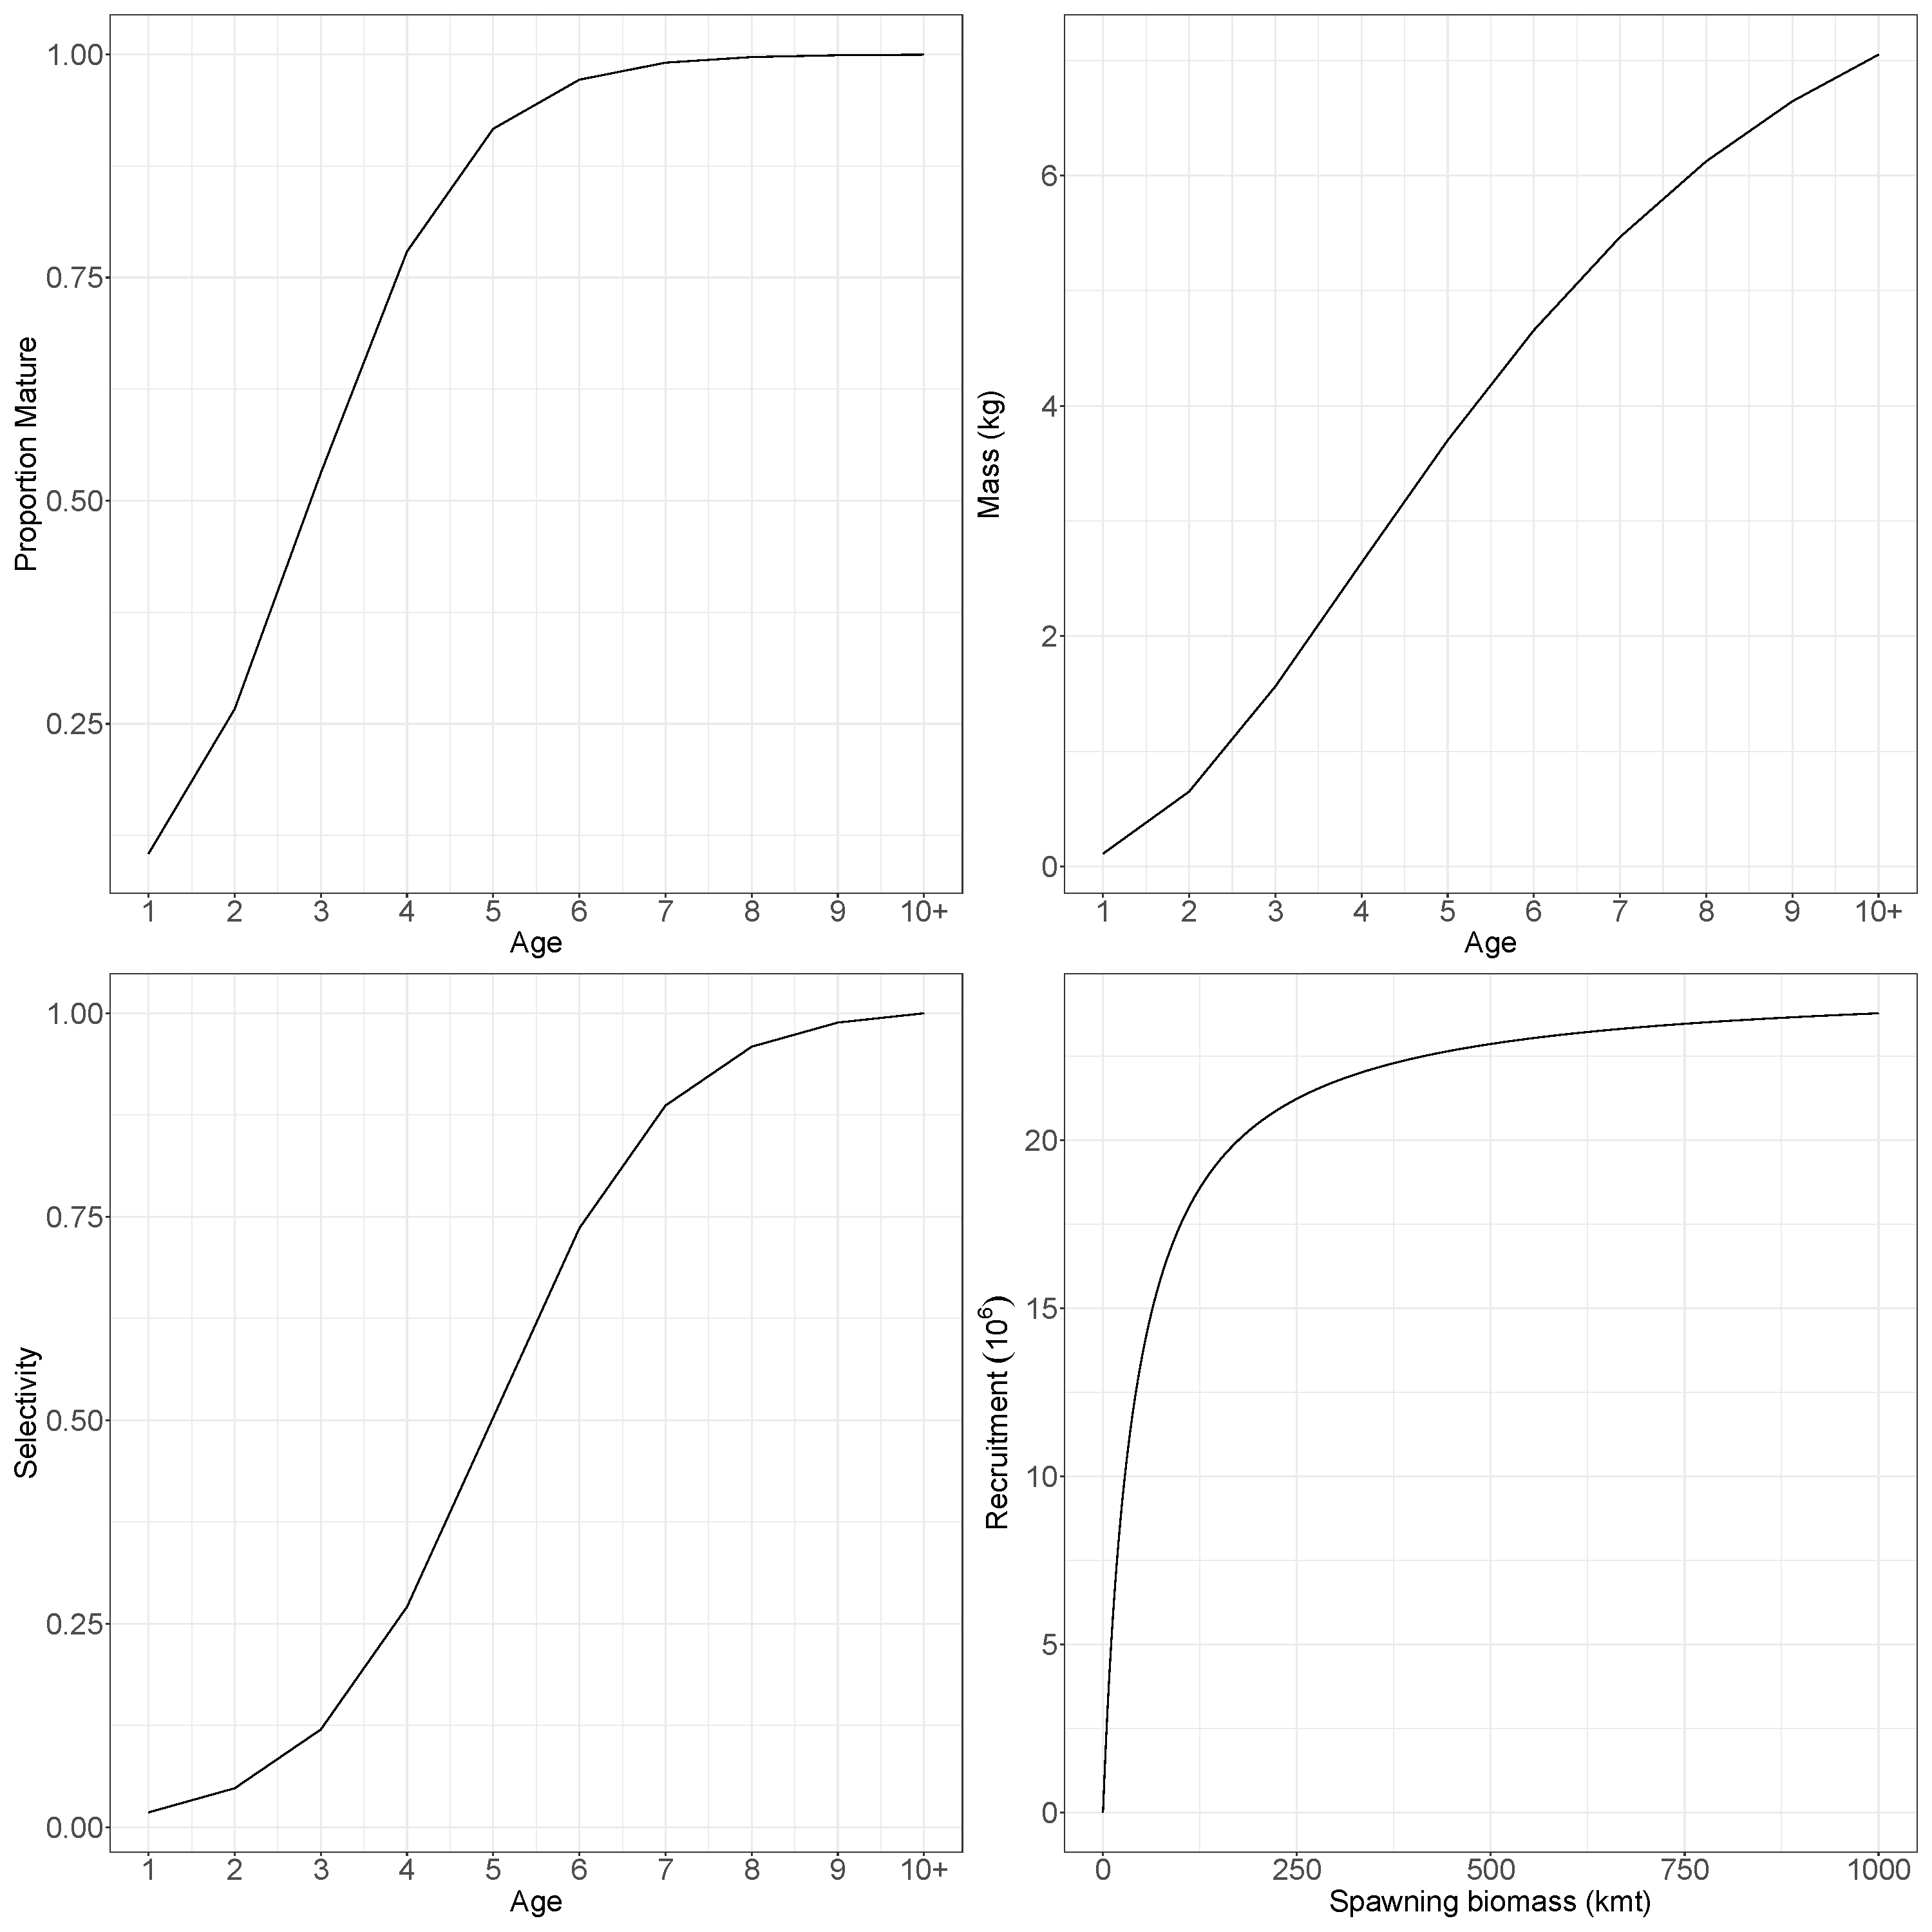
\includegraphics[width = \textwidth]{om_input_plots_figure}
\end{center}
\caption{The proportion mature at age, weight at age, fleet and index selectivity at age, and Beverton-Holt stock-recruit relationship assumed for the population in all operating models. For operating models with random effects on fleet selectivity, this represents the selectivity at the mean of the random effects.}\label{om_inputs_fig}
\end{figure}

\begin{landscape}
\DIFaddbegin \begin{figure}
\begin{center}
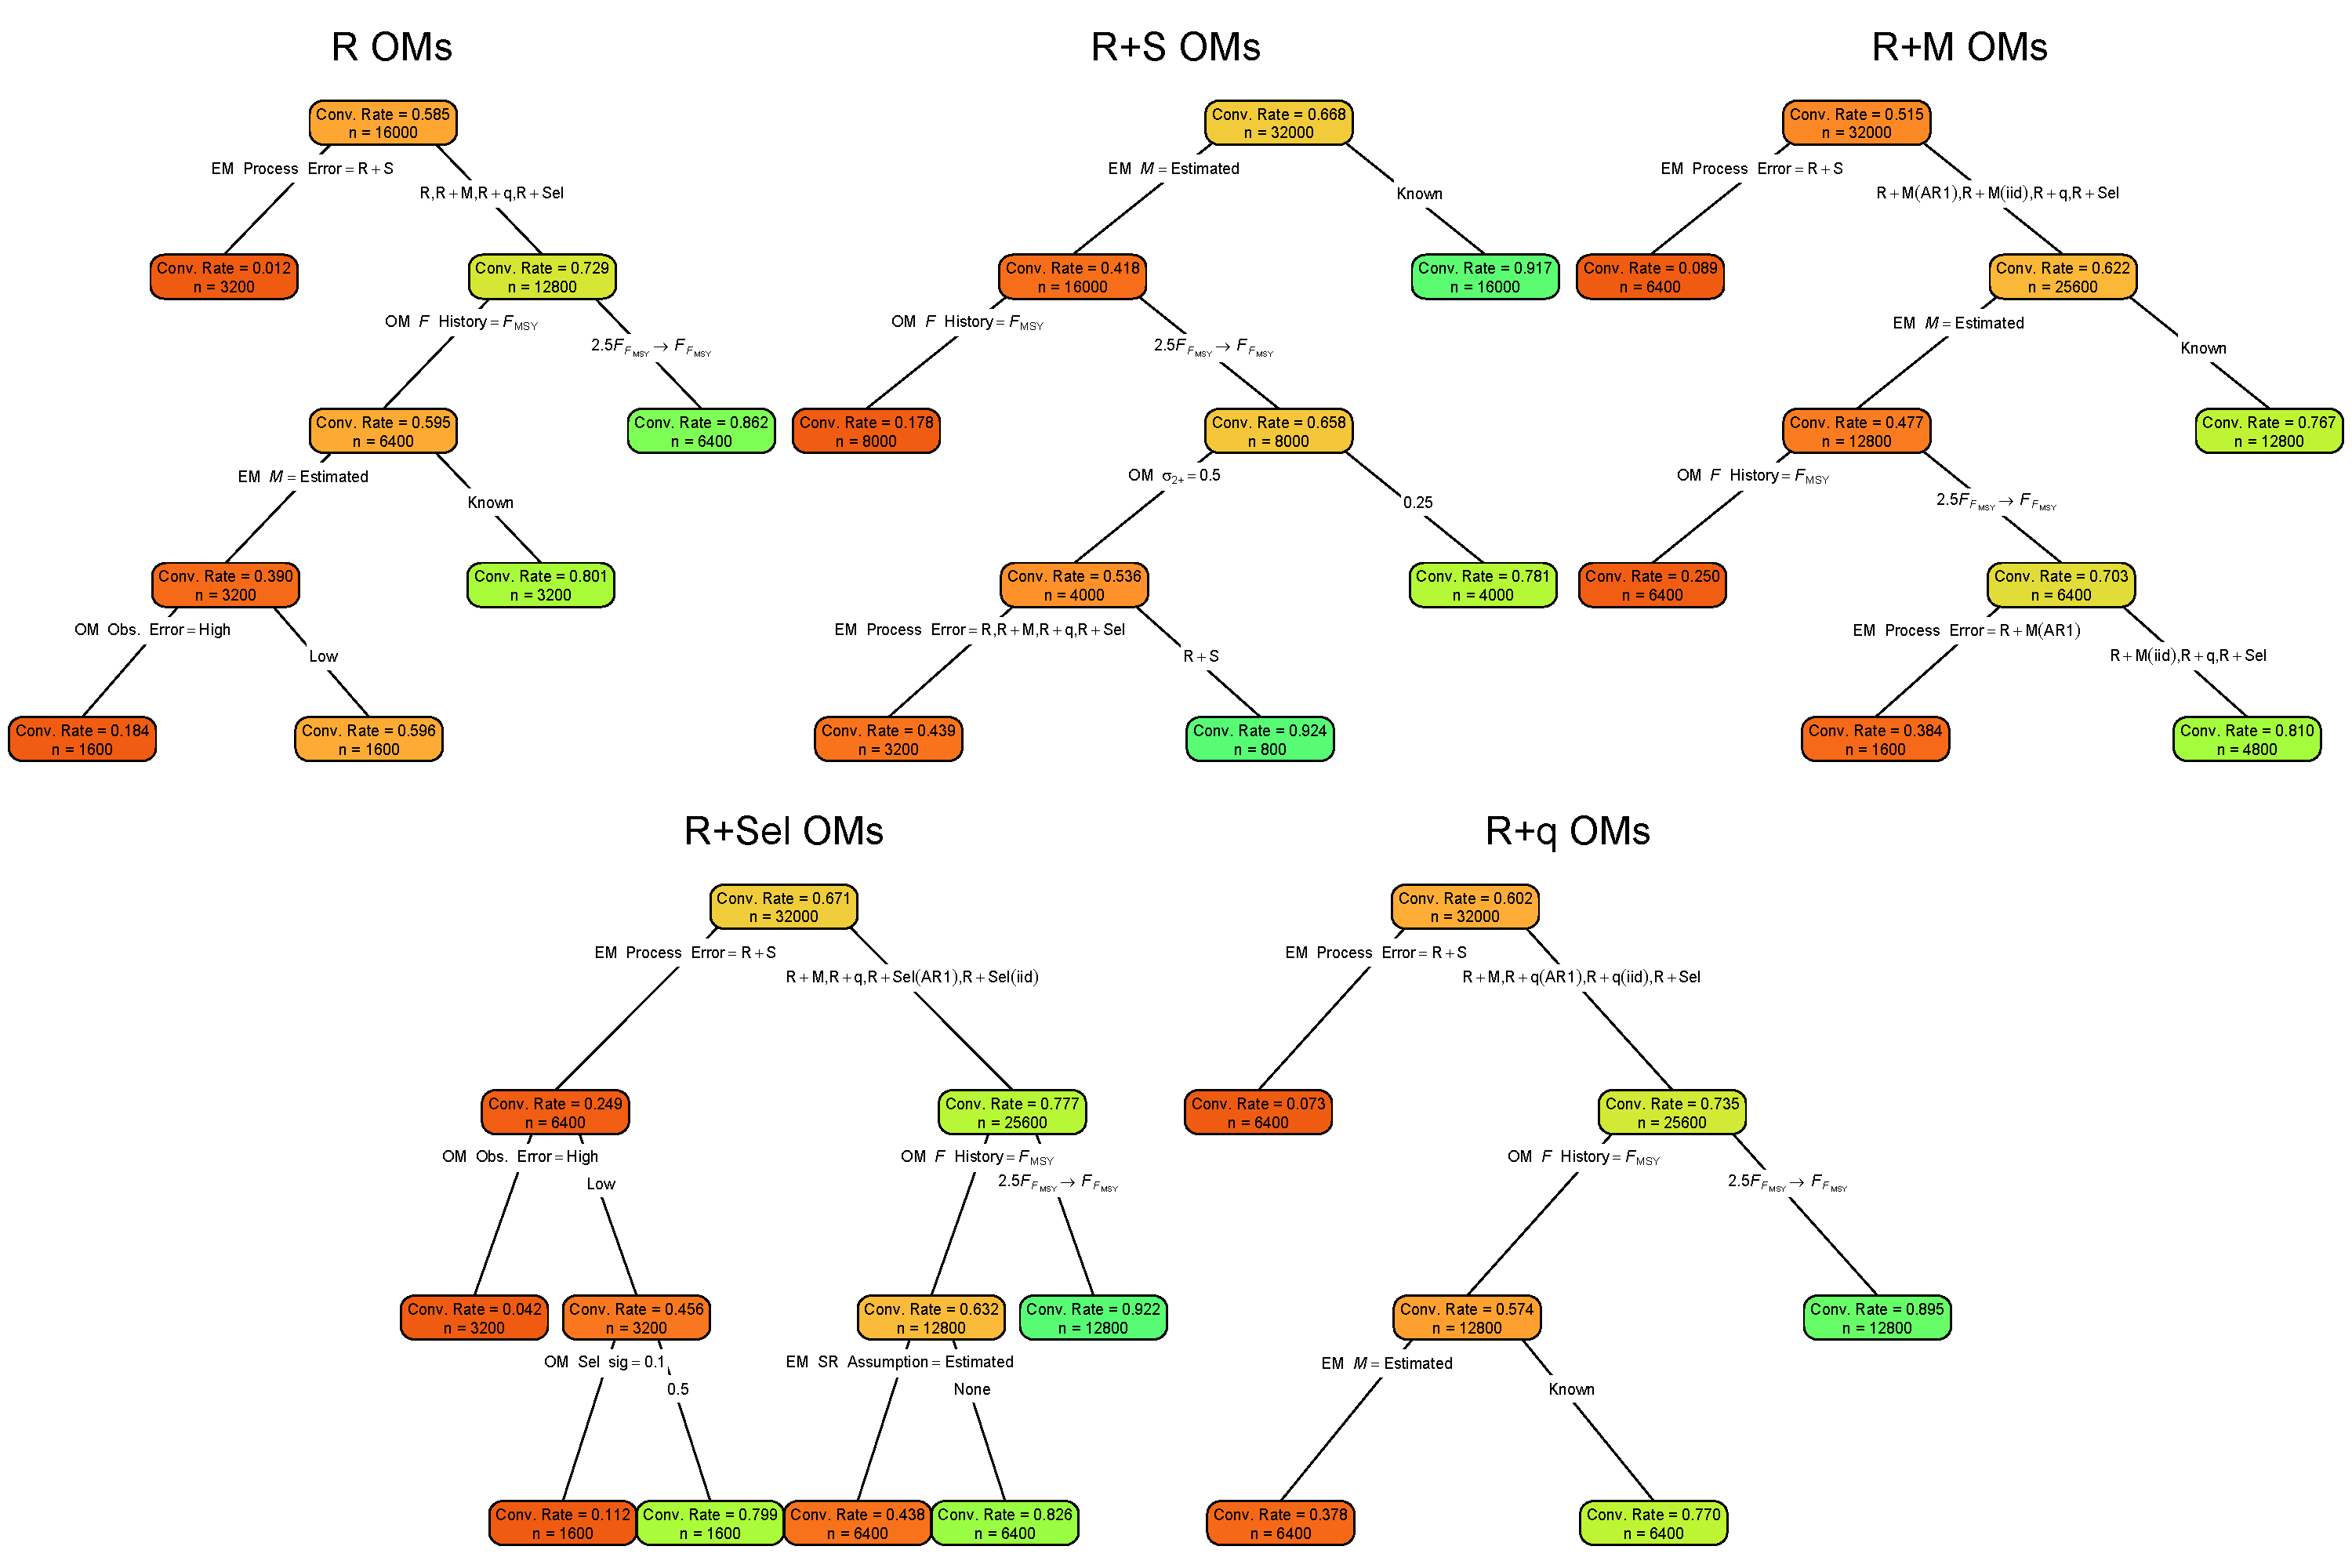
\includegraphics[width = 1.4\textwidth]{convergence_gradient_classification_plots}
\end{center}
\caption{\DIFaddFL{Classification trees indicating primary factors determining convergence as defined by a maximum absolute gradient < $10^{-6}$ for R, R+S, R+M, R+Sel and R+q OMs. Lower or higher convergence rates are indicated by more red or green polygons, respectively}}\label{conv_gradient_class}
\end{figure}
\end{landscape}

\begin{landscape}
\begin{figure}
\begin{center}
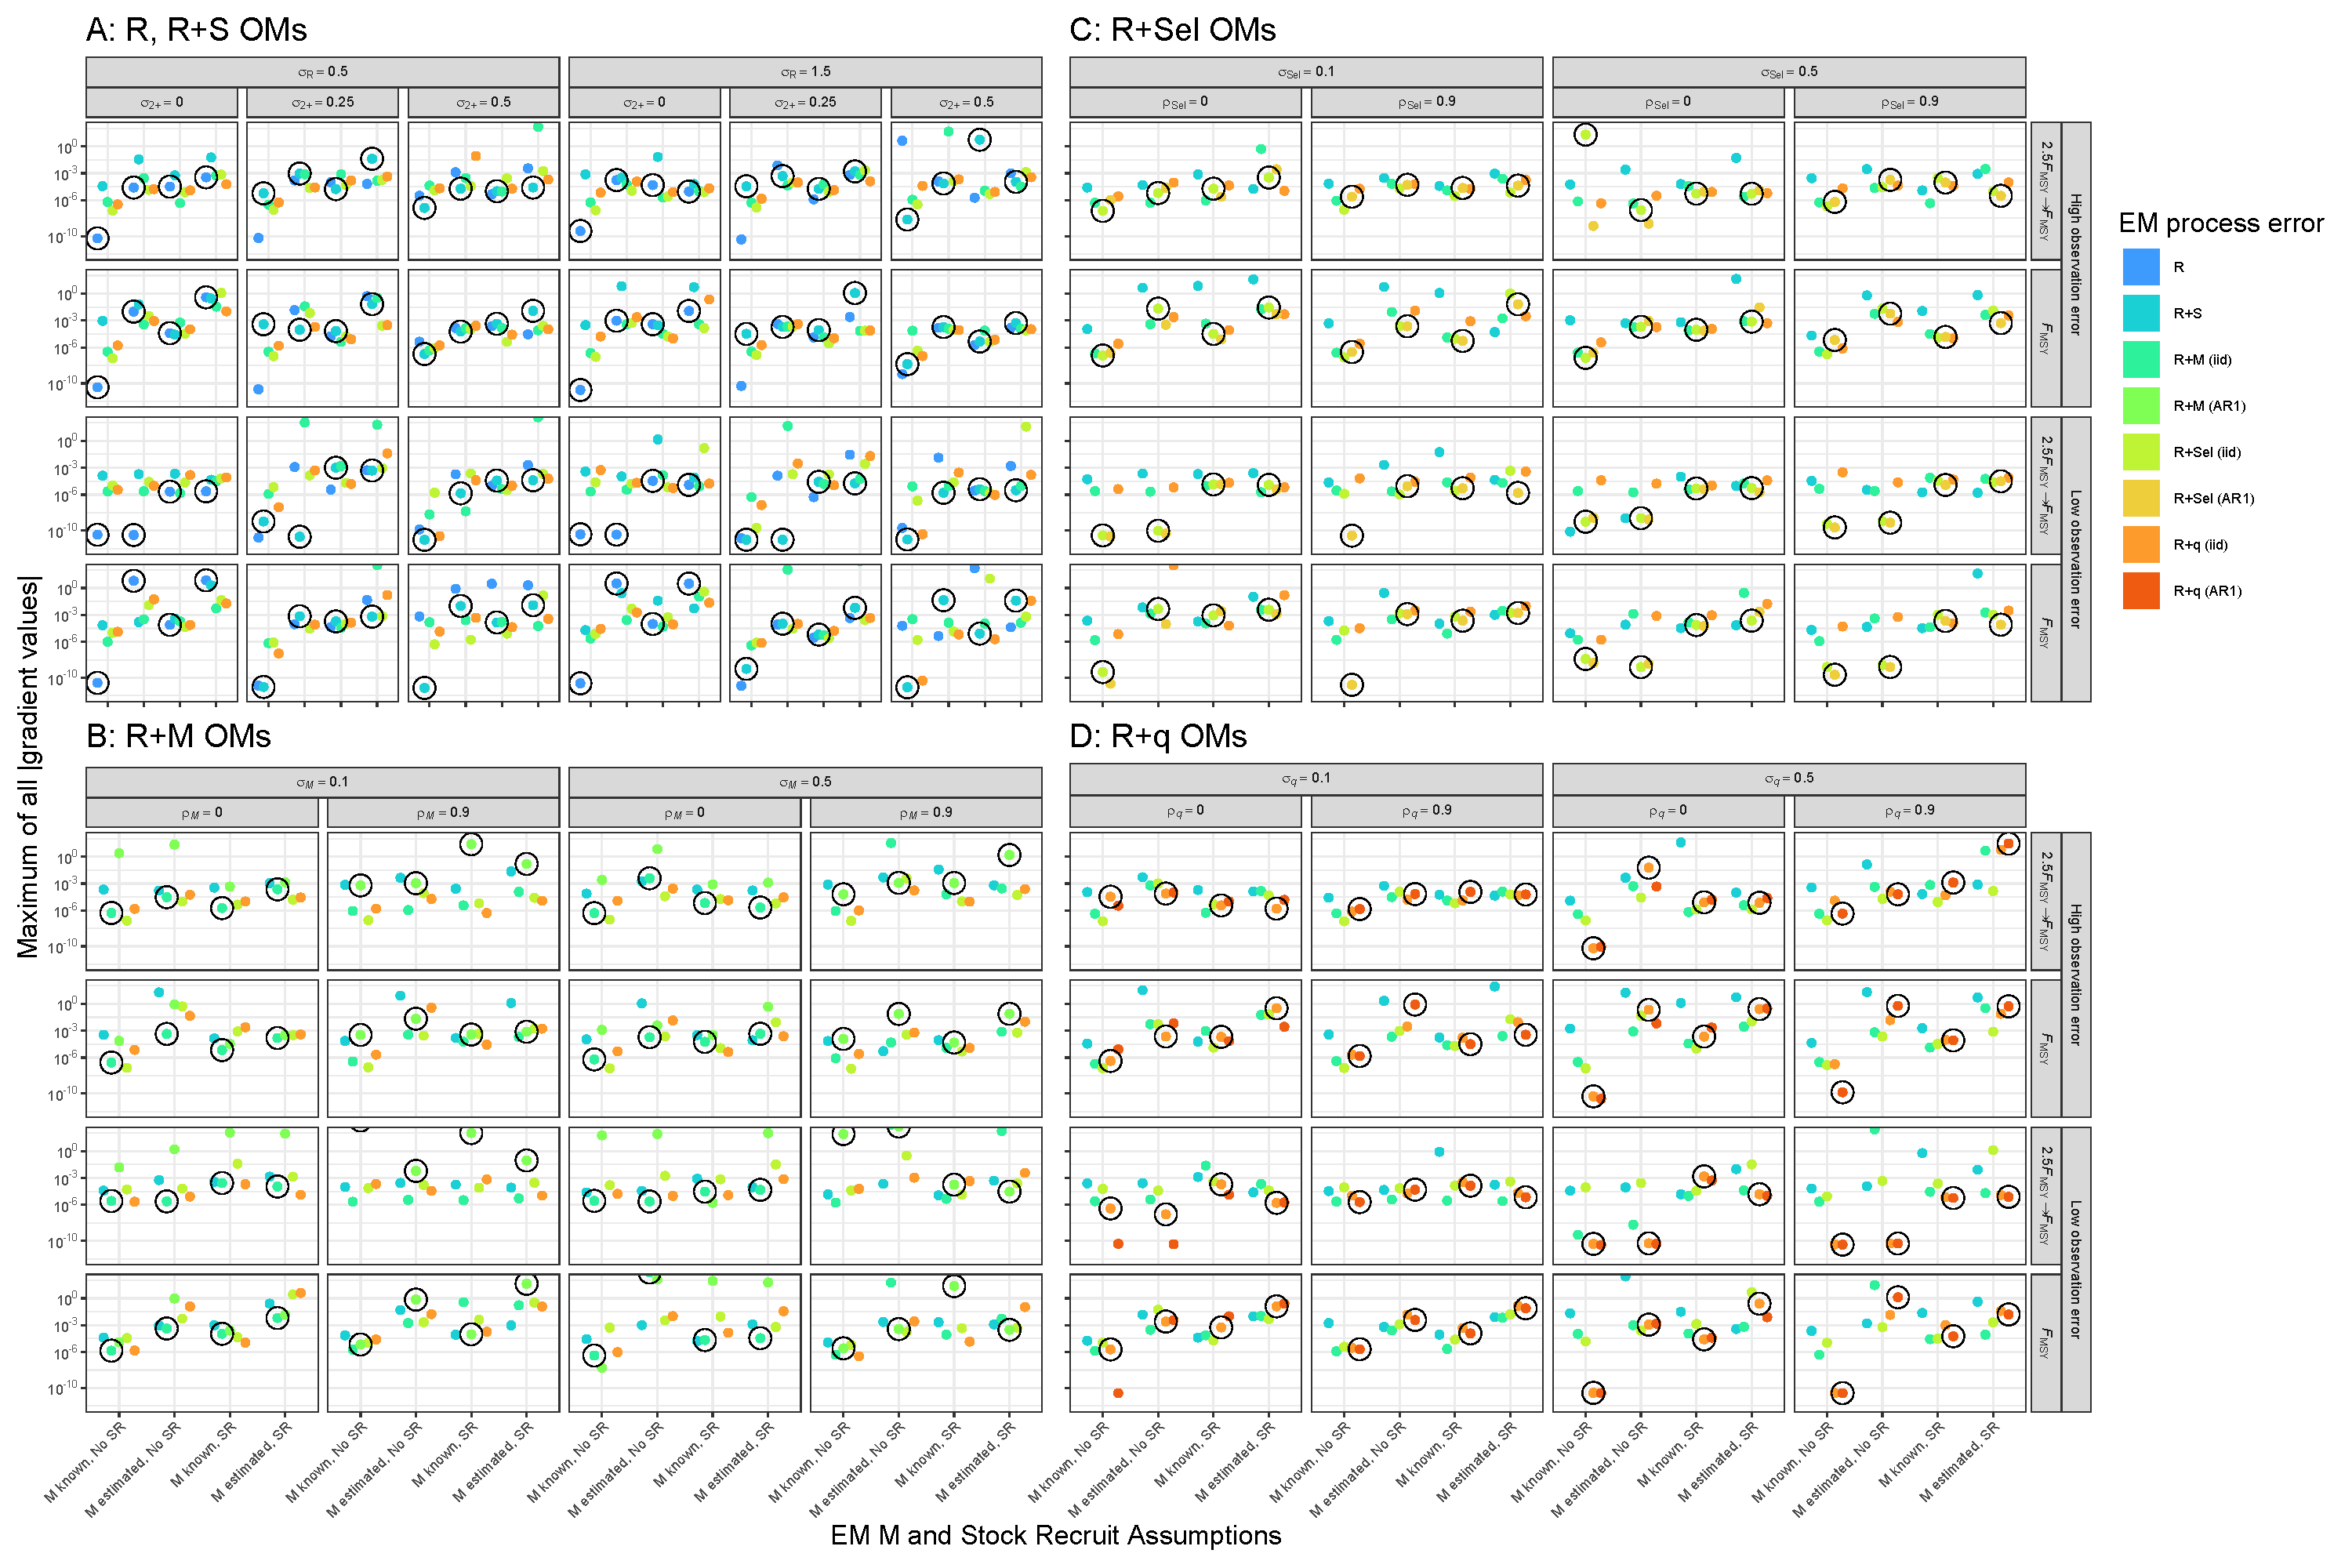
\includegraphics[width = 1.4\textwidth]{hess_grad_convergence_plots}
\end{center}
\caption{\DIFaddFL{The maximum of the absolute values of all gradient values for all fits that provided hessian-based standard errors across all simuated data sets of a given OM configuration (A: R and R+S, B: R+M, C: R+Sel, or D: R+q).  Results are conditional on EM fits with alternative process error type (colored points and lines), median natural mortality (estimated or known) and recruitment assumptions (Beverton-Holt stock-recruit relationship or not). Circled values indicate results where the EM process error structure matches that of the operating model and vertical lines represent 95\% confidence intervals.}}\label{hess_grad}
\end{figure}
\end{landscape}

\DIFaddend \begin{table}
\DIFaddbeginFL \caption{\DIFaddFL{For each OM process error type (columns), percent reduction in deviance for linear regression models fit to errors in estimation measured by Eq. \ref{bias_regression_response} for the terminal year fully-selected fishing mortality with each OM and EM factor (rows) included individually, combined, and with second and third order interactions.}}\label{bias_F_PRD_table}
{\begin{center}
\begin{tabular}{lrrrrr}
\hline\hline
\multicolumn{1}{l}{\DIFaddFL{Factor}}&\multicolumn{1}{c}{\DIFaddFL{R}}&\multicolumn{1}{c}{\DIFaddFL{R+S}}&\multicolumn{1}{c}{\DIFaddFL{R+M}}&\multicolumn{1}{c}{\DIFaddFL{R+Sel}}&\multicolumn{1}{c}{\DIFaddFL{R+q}}\tabularnewline
\hline
\DIFaddFL{EM $M$ Assumption}& \DIFaddFL{2.26}& \DIFaddFL{1.33}& \DIFaddFL{1.26}& \DIFaddFL{2.93}& \DIFaddFL{3.26}\tabularnewline
\DIFaddFL{EM SR assumption}& \DIFaddFL{0.11}& \DIFaddFL{0.07}& \DIFaddFL{0.08}& \DIFaddFL{0.07}& \DIFaddFL{0.09}\tabularnewline
\DIFaddFL{EM Process Error}& \DIFaddFL{0.46}& \DIFaddFL{4.18}& \DIFaddFL{0.38}& \DIFaddFL{0.13}& \DIFaddFL{1.02}\tabularnewline
\DIFaddFL{OM Obs. Error}& \DIFaddFL{1.61}& \DIFaddFL{0.06}& \DIFaddFL{0.86}& \DIFaddFL{0.41}&\DIFaddFL{\textless  0.01}\tabularnewline
\DIFaddFL{OM $F$ History}& \DIFaddFL{2.49}& \DIFaddFL{3.23}& \DIFaddFL{1.42}& \DIFaddFL{3.22}& \DIFaddFL{4.55}\tabularnewline
\DIFaddFL{OM $\sigma_R$}& \DIFaddFL{0.02}& \DIFaddFL{0.02}&\DIFaddFL{--}&\DIFaddFL{--}&\DIFaddFL{--}\tabularnewline
\DIFaddFL{OM $\sigma_{2+}$ }&\DIFaddFL{--}& \DIFaddFL{0.87}&\DIFaddFL{--}&\DIFaddFL{--}&\DIFaddFL{--}\tabularnewline
\DIFaddFL{OM $\sigma_M$}&\DIFaddFL{--}&\DIFaddFL{--}& \DIFaddFL{0.16}&\DIFaddFL{--}&\DIFaddFL{--}\tabularnewline
\DIFaddFL{OM $\rho_R$}&\DIFaddFL{--}&\DIFaddFL{--}& \DIFaddFL{0.01}&\DIFaddFL{--}&\DIFaddFL{--}\tabularnewline
\DIFaddFL{OM $\sigma_{Sel}$}&\DIFaddFL{--}&\DIFaddFL{--}&\DIFaddFL{--}& \DIFaddFL{0.24}&\DIFaddFL{--}\tabularnewline
\DIFaddFL{OM $\rho_{Sel}$}&\DIFaddFL{--}&\DIFaddFL{--}&\DIFaddFL{--}& \DIFaddFL{0.05}&\DIFaddFL{--}\tabularnewline
\DIFaddFL{OM $\sigma_q$}&\DIFaddFL{--}&\DIFaddFL{--}&\DIFaddFL{--}&\DIFaddFL{--}& \DIFaddFL{1.03}\tabularnewline
\DIFaddFL{OM $\rho_q$}&\DIFaddFL{--}&\DIFaddFL{--}&\DIFaddFL{--}&\DIFaddFL{--}& \DIFaddFL{0.05}\tabularnewline
\DIFaddFL{All factors}& \DIFaddFL{7.42}& \DIFaddFL{9.96}& \DIFaddFL{4.37}& \DIFaddFL{7.26}&\DIFaddFL{10.43}\tabularnewline
\DIFaddFL{+ All Two Way}&\DIFaddFL{17.63}&\DIFaddFL{25.76}&\DIFaddFL{10.94}&\DIFaddFL{13.88}&\DIFaddFL{22.07}\tabularnewline
\DIFaddFL{+ All Three Way}&\DIFaddFL{22.97}&\DIFaddFL{37.03}&\DIFaddFL{14.74}&\DIFaddFL{17.32}&\DIFaddFL{30.74}\tabularnewline
\hline
\end{tabular}\end{center}
}
\end{table}

\begin{table}
\caption{\DIFaddFL{For each OM process error type (columns), percent reduction in deviance for linear regression models fit to errors in estimation measured by Eq. \ref{bias_regression_response} for the terminal year recruitment with each OM and EM factor (rows) included individually, combined, and with second and third order interactions.}}\label{bias_R_PRD_table}
{\begin{center}
\begin{tabular}{lrrrrr}
\hline\hline
\multicolumn{1}{l}{\DIFaddFL{Factor}}&\multicolumn{1}{c}{\DIFaddFL{R}}&\multicolumn{1}{c}{\DIFaddFL{R+S}}&\multicolumn{1}{c}{\DIFaddFL{R+M}}&\multicolumn{1}{c}{\DIFaddFL{R+Sel}}&\multicolumn{1}{c}{\DIFaddFL{R+q}}\tabularnewline
\hline
\DIFaddFL{EM $M$ Assumption}& \DIFaddFL{1.96}& \DIFaddFL{0.40}& \DIFaddFL{0.69}& \DIFaddFL{3.52}& \DIFaddFL{3.03}\tabularnewline
\DIFaddFL{EM SR assumption}& \DIFaddFL{0.06}& \DIFaddFL{0.02}& \DIFaddFL{0.05}& \DIFaddFL{0.02}& \DIFaddFL{0.05}\tabularnewline
\DIFaddFL{EM Process Error}& \DIFaddFL{0.39}& \DIFaddFL{4.74}& \DIFaddFL{0.41}& \DIFaddFL{0.12}& \DIFaddFL{1.16}\tabularnewline
\DIFaddFL{OM Obs. Error}& \DIFaddFL{1.47}& \DIFaddFL{0.08}& \DIFaddFL{0.64}& \DIFaddFL{0.18}&\DIFaddFL{\textless  0.01}\tabularnewline
\DIFaddFL{OM $F$ History}& \DIFaddFL{2.54}& \DIFaddFL{2.66}& \DIFaddFL{1.11}& \DIFaddFL{4.18}& \DIFaddFL{5.06}\tabularnewline
\DIFaddFL{OM $\sigma_R$}& \DIFaddFL{0.03}& \DIFaddFL{0.01}&\DIFaddFL{--}&\DIFaddFL{--}&\DIFaddFL{--}\tabularnewline
\DIFaddFL{OM $\sigma_{2+}$ }&\DIFaddFL{--}& \DIFaddFL{1.05}&\DIFaddFL{--}&\DIFaddFL{--}&\DIFaddFL{--}\tabularnewline
\DIFaddFL{OM $\sigma_M$}&\DIFaddFL{--}&\DIFaddFL{--}& \DIFaddFL{0.36}&\DIFaddFL{--}&\DIFaddFL{--}\tabularnewline
\DIFaddFL{OM $\rho_R$}&\DIFaddFL{--}&\DIFaddFL{--}& \DIFaddFL{0.02}&\DIFaddFL{--}&\DIFaddFL{--}\tabularnewline
\DIFaddFL{OM $\sigma_{Sel}$}&\DIFaddFL{--}&\DIFaddFL{--}&\DIFaddFL{--}& \DIFaddFL{0.23}&\DIFaddFL{--}\tabularnewline
\DIFaddFL{OM $\rho_{Sel}$}&\DIFaddFL{--}&\DIFaddFL{--}&\DIFaddFL{--}& \DIFaddFL{0.06}&\DIFaddFL{--}\tabularnewline
\DIFaddFL{OM $\sigma_q$}&\DIFaddFL{--}&\DIFaddFL{--}&\DIFaddFL{--}&\DIFaddFL{--}& \DIFaddFL{1.09}\tabularnewline
\DIFaddFL{OM $\rho_q$}&\DIFaddFL{--}&\DIFaddFL{--}&\DIFaddFL{--}&\DIFaddFL{--}& \DIFaddFL{0.06}\tabularnewline
\DIFaddFL{All factors}& \DIFaddFL{6.90}& \DIFaddFL{9.01}& \DIFaddFL{3.43}& \DIFaddFL{8.58}&\DIFaddFL{10.90}\tabularnewline
\DIFaddFL{+ All Two Way}&\DIFaddFL{16.48}&\DIFaddFL{24.64}& \DIFaddFL{9.73}&\DIFaddFL{15.76}&\DIFaddFL{22.75}\tabularnewline
\DIFaddFL{+ All Three Way}&\DIFaddFL{21.46}&\DIFaddFL{35.60}&\DIFaddFL{13.56}&\DIFaddFL{19.07}&\DIFaddFL{31.15}\tabularnewline
\hline
\end{tabular}\end{center}
}
\end{table}

\begin{landscape}
\begin{figure}
\begin{center}
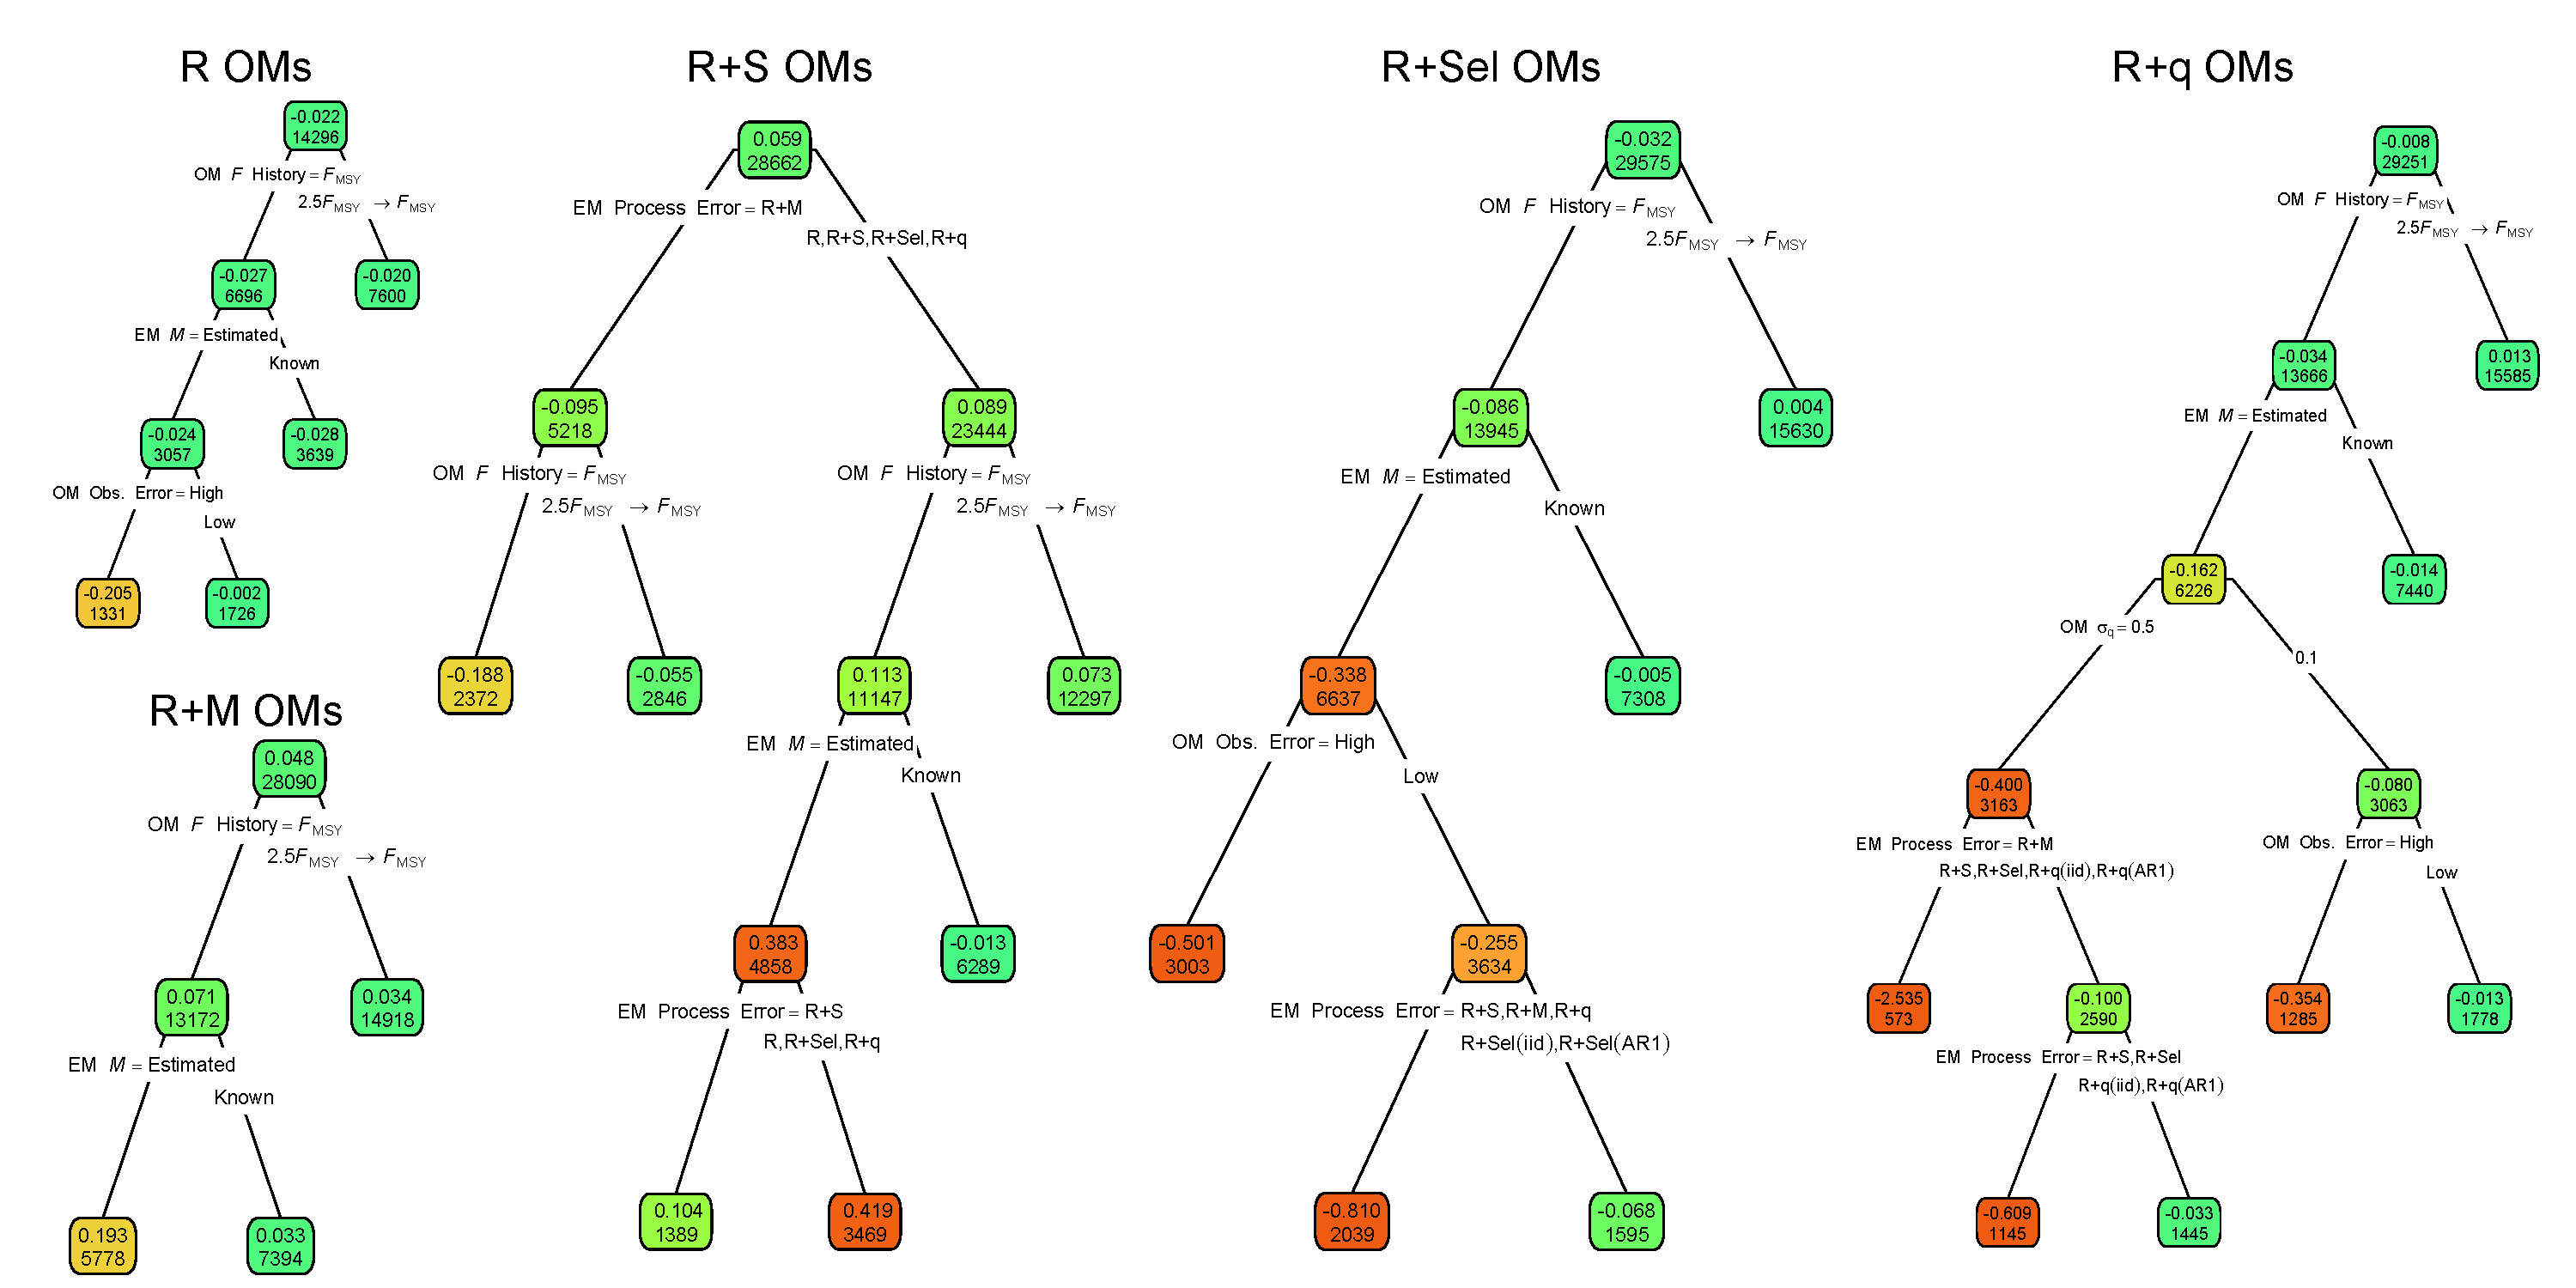
\includegraphics[width = 1.4\textwidth]{F_bias_regtree_plots}
\end{center}
\caption{\DIFaddFL{Regression trees indicating primary factors determining reductions in sums of squares of errors in estimation measured by Eq. \ref{bias_regression_response} for terminal year fully-selected fishing mortality for R+S, R+M, R+Sel and R+q OMs. Each node shows the median error (top) and number of observations (bottom) for the corresponding subset. Median errors closer to or further from zero are indicated by more green or red polygons, respectively.}}\label{F_bias_regtree}
\end{figure}
\end{landscape}

\begin{landscape}
\begin{figure}
\begin{center}
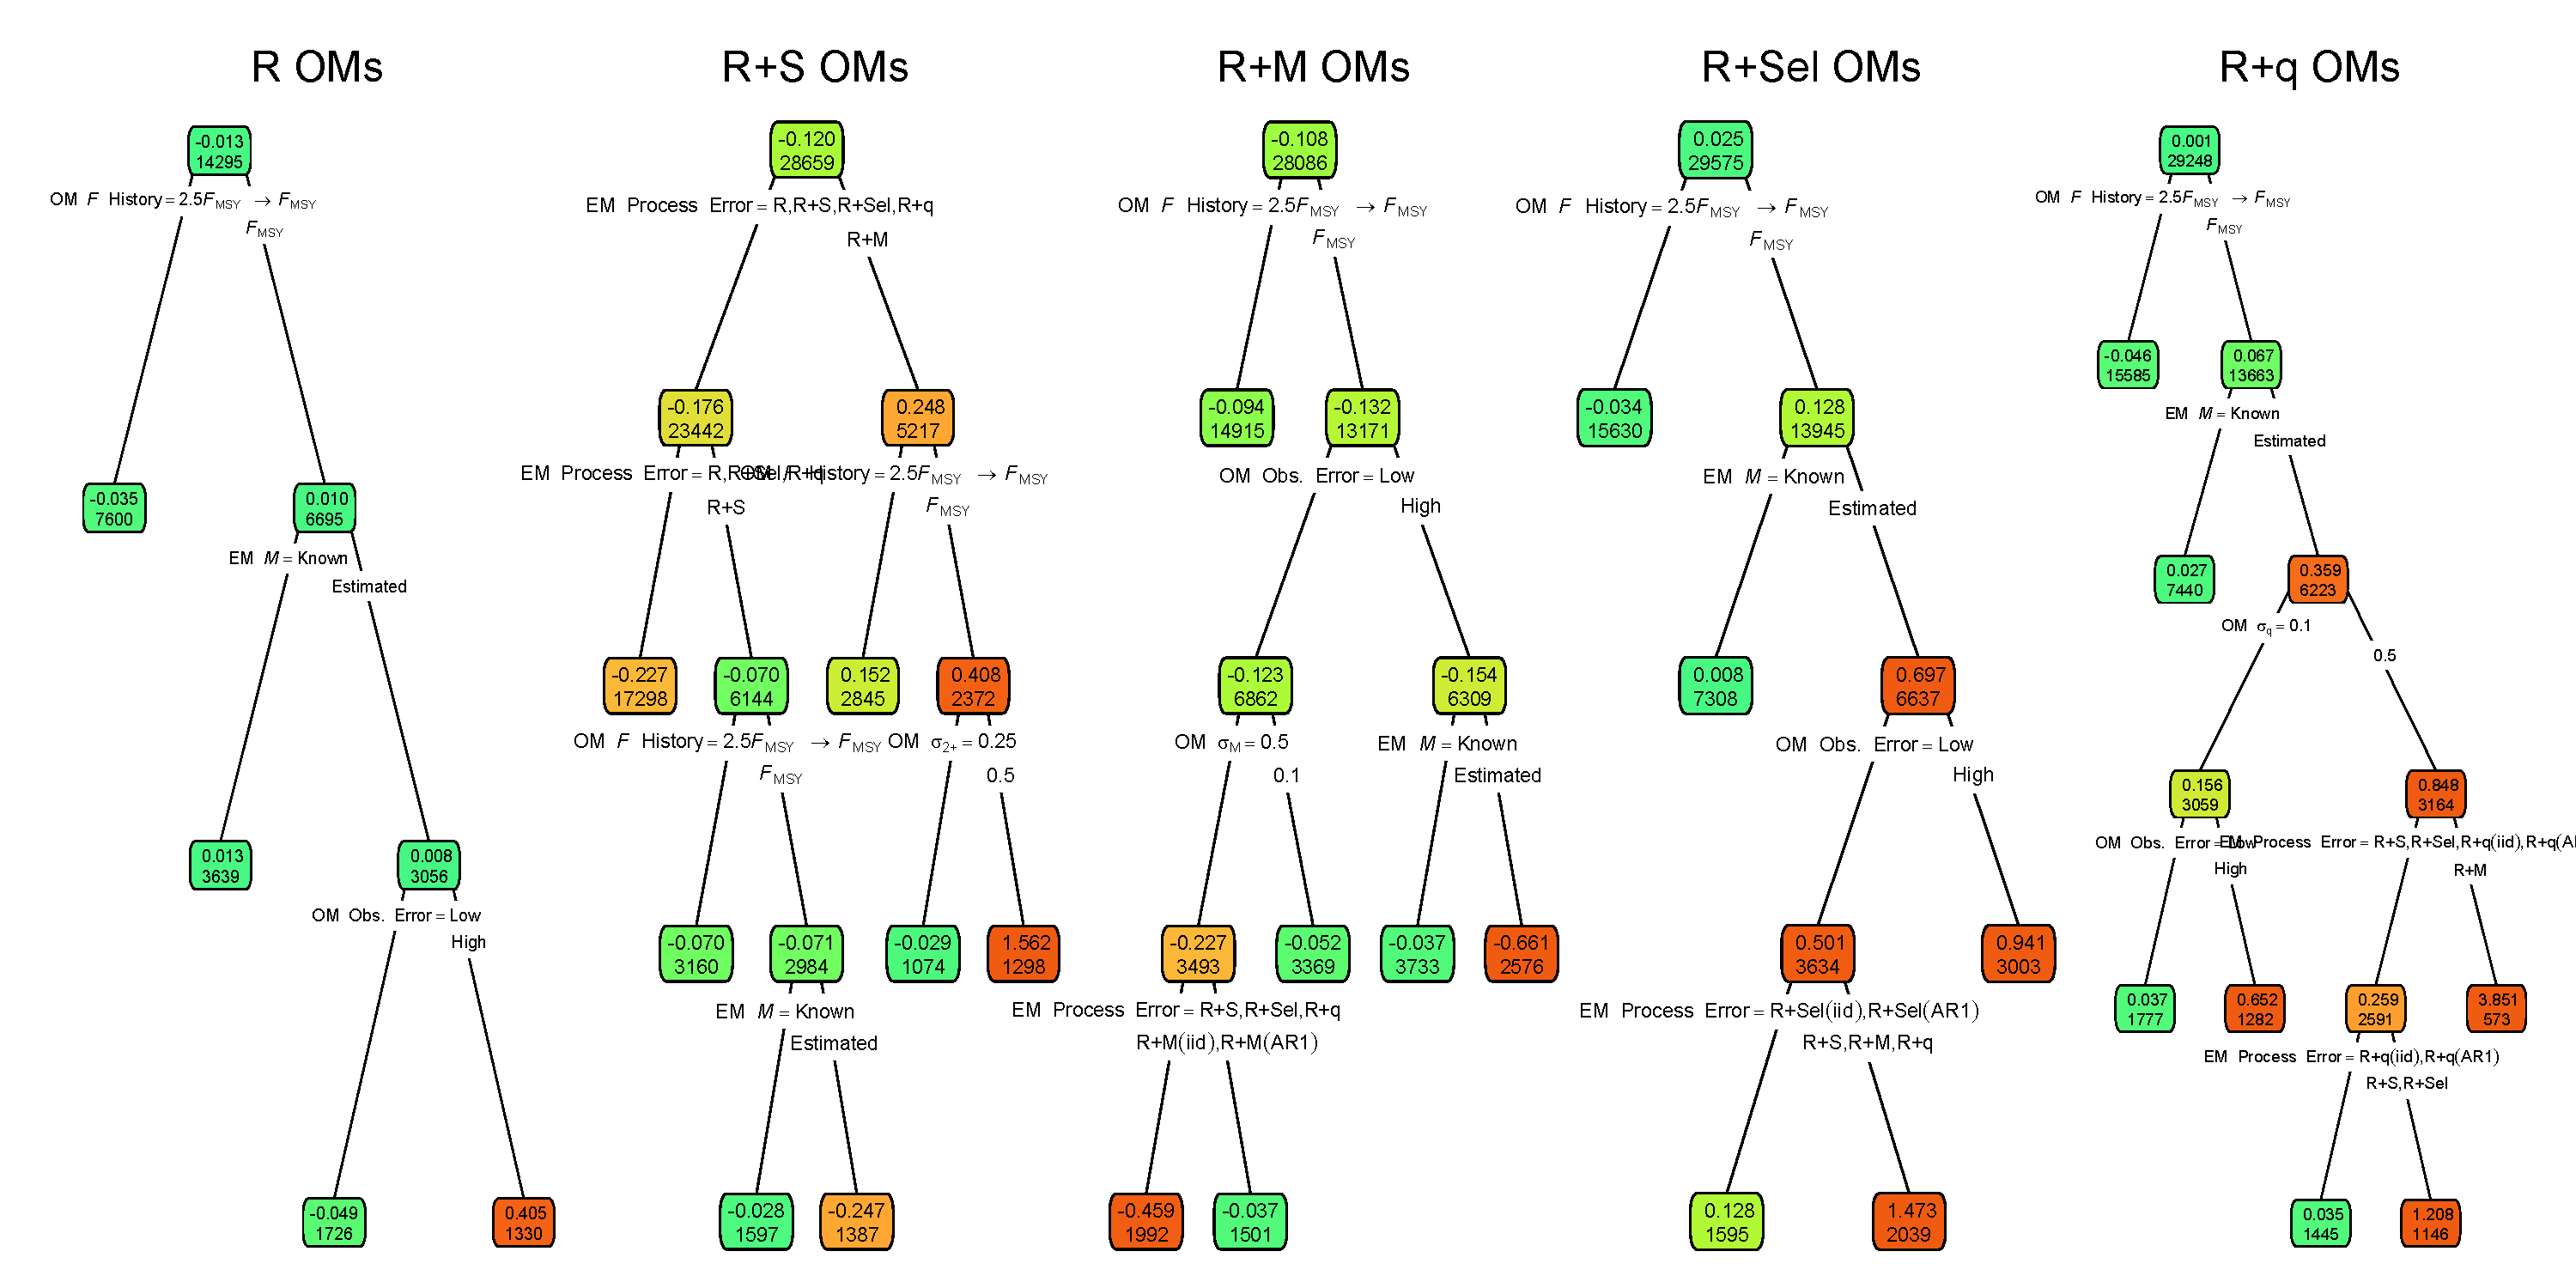
\includegraphics[width = 1.4\textwidth]{R_bias_regtree_plots}
\end{center}
\caption{\DIFaddFL{Regression trees indicating primary factors determining reductions in sums of squares of errors in estimation measured by Eq. \ref{bias_regression_response} for terminal year recruitment for R+S, R+M, R+Sel and R+q OMs. Each node shows the median error (top) and number of observations (bottom) for the corresponding subset. Median errors closer to or further from zero are indicated by more green or red polygons, respectively.}}\label{R_bias_regtree}
\end{figure}
\end{landscape}

\clearpage

\begin{landscape}
\begin{figure}
\begin{center}
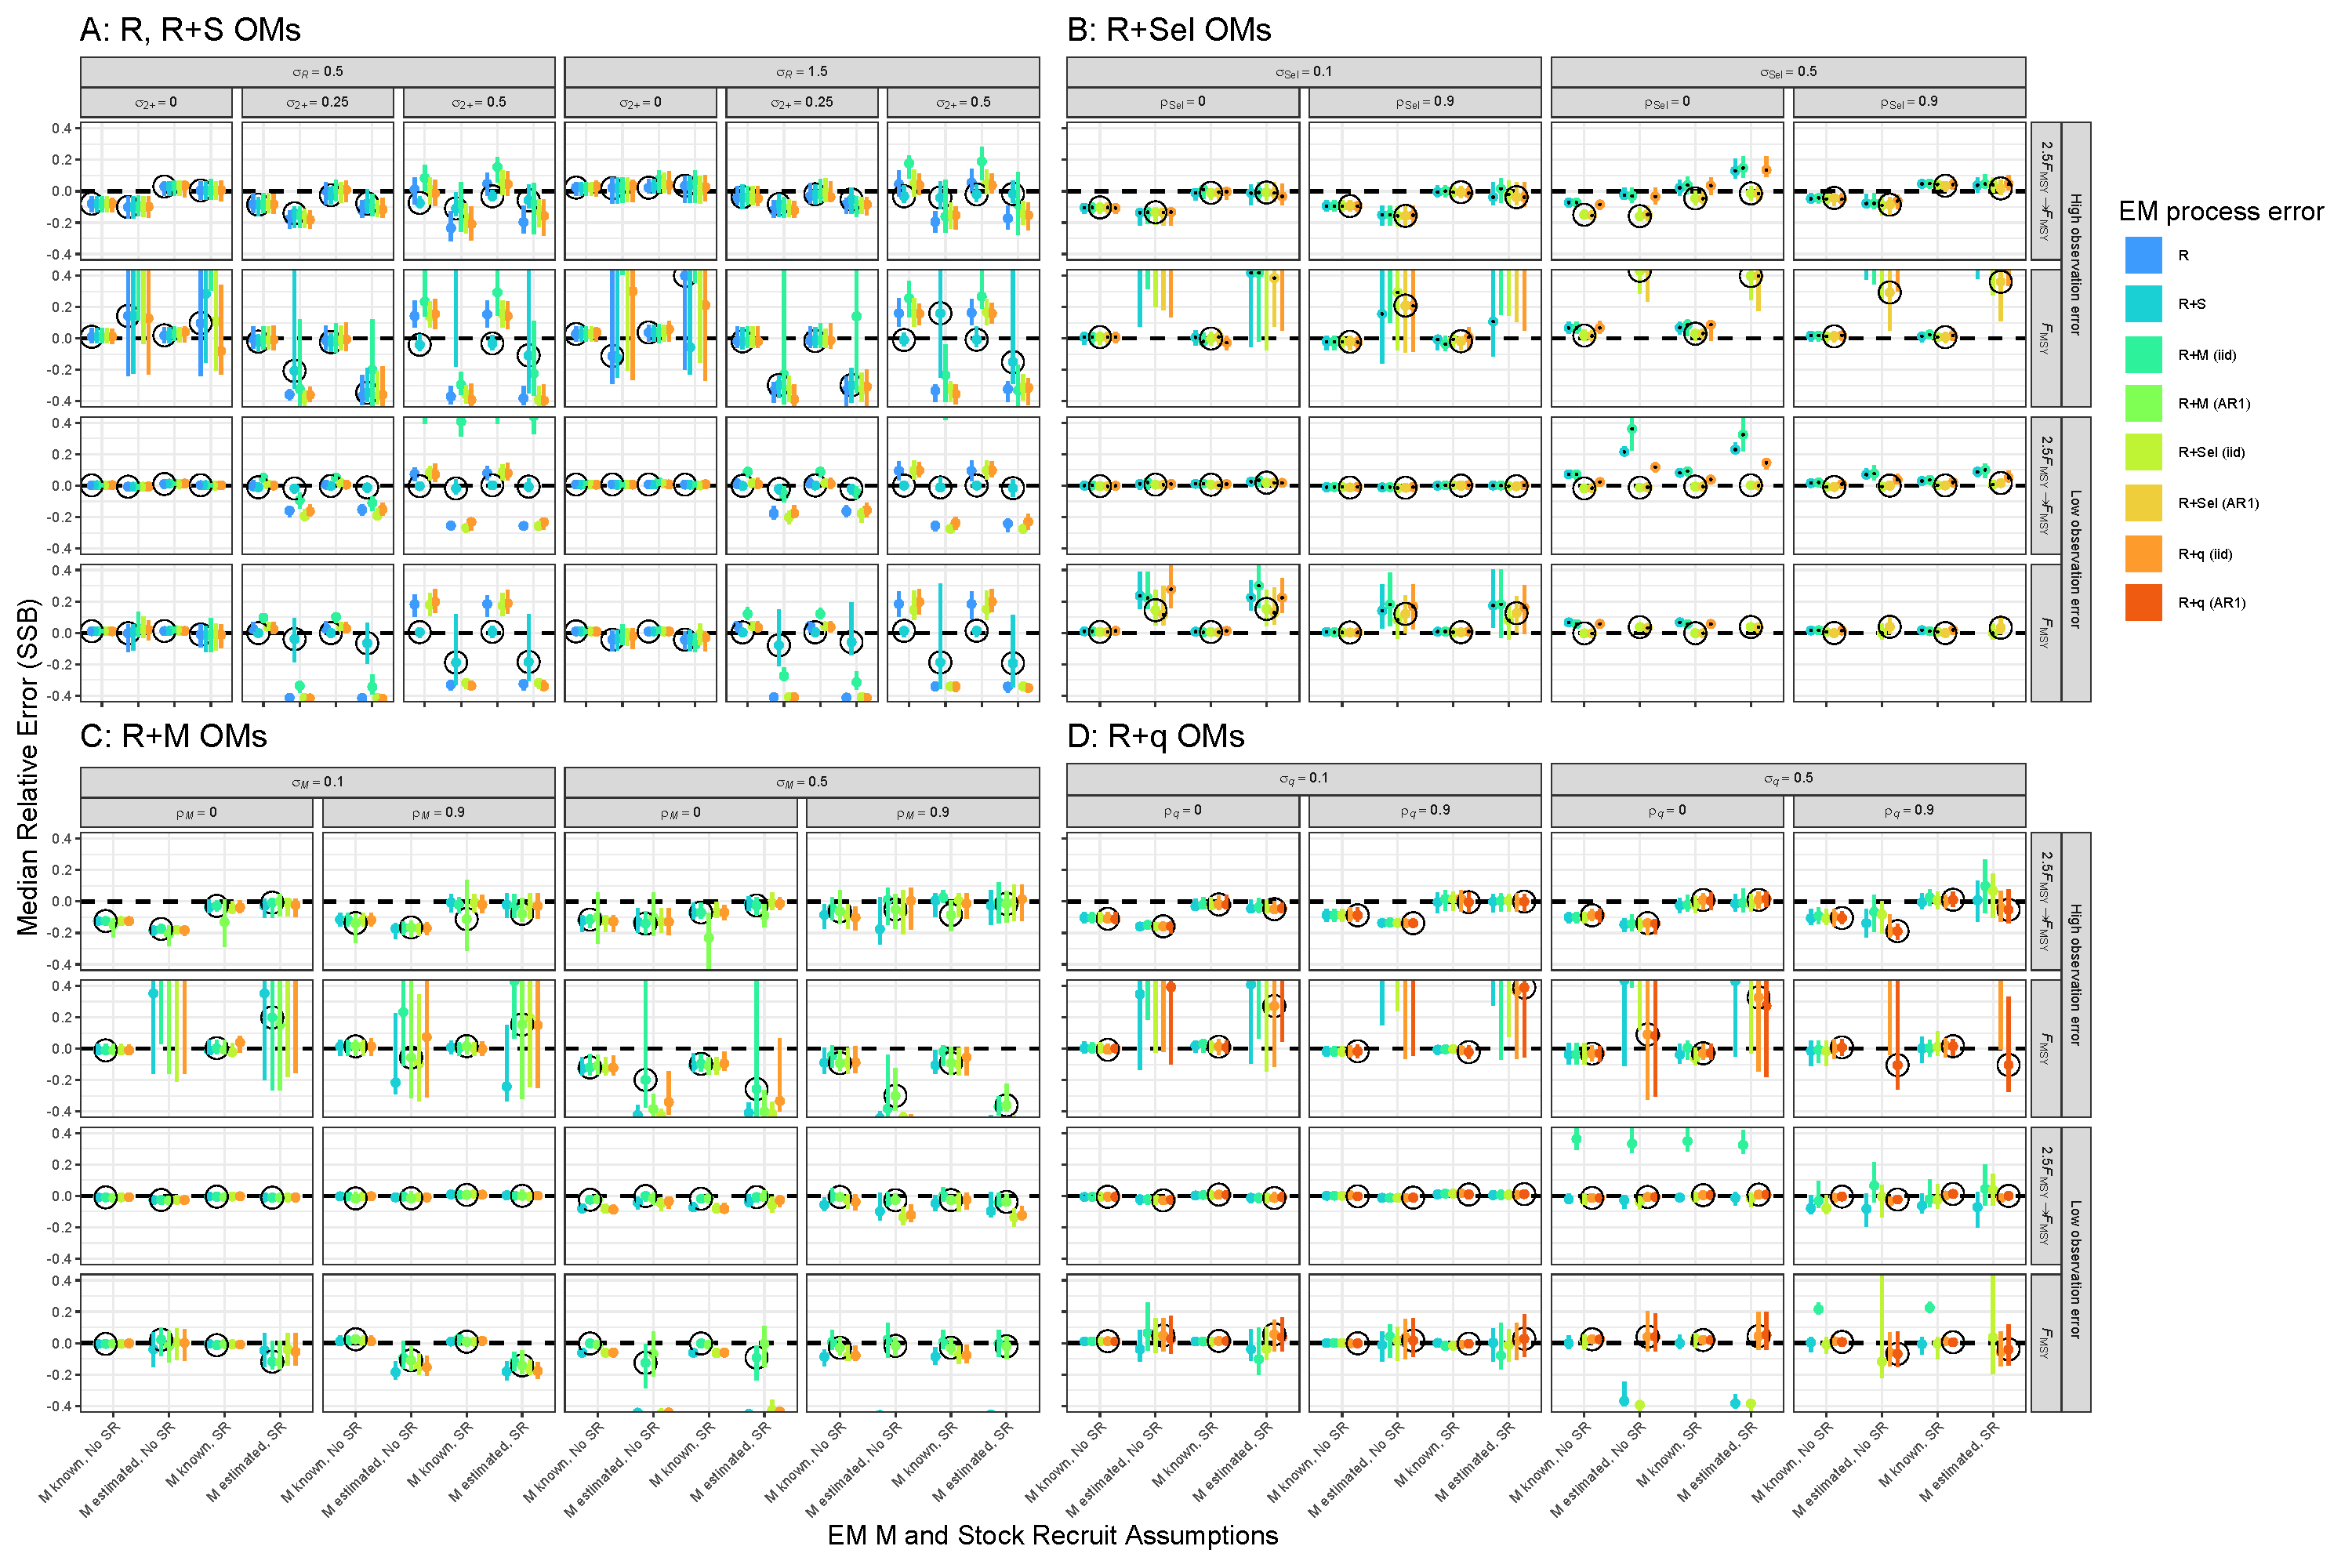
\includegraphics[width = 1.4\textwidth]{term_SSB_bias_plots}
\end{center}
\caption{\DIFaddFL{Median relative error of terminal year SSB for estimating models fitted to data sets simulated with alternative process error structures: R and R+S (A), R+Sel (B), R+M (C), or R+q (D). Circled values indicate results where the EM process error structure matches that of the operating model and vertical lines represent 95\% confidence intervals.}}\label{SSB_rel_error}
\end{figure}
\end{landscape}

\begin{landscape}
\begin{figure}
\begin{center}
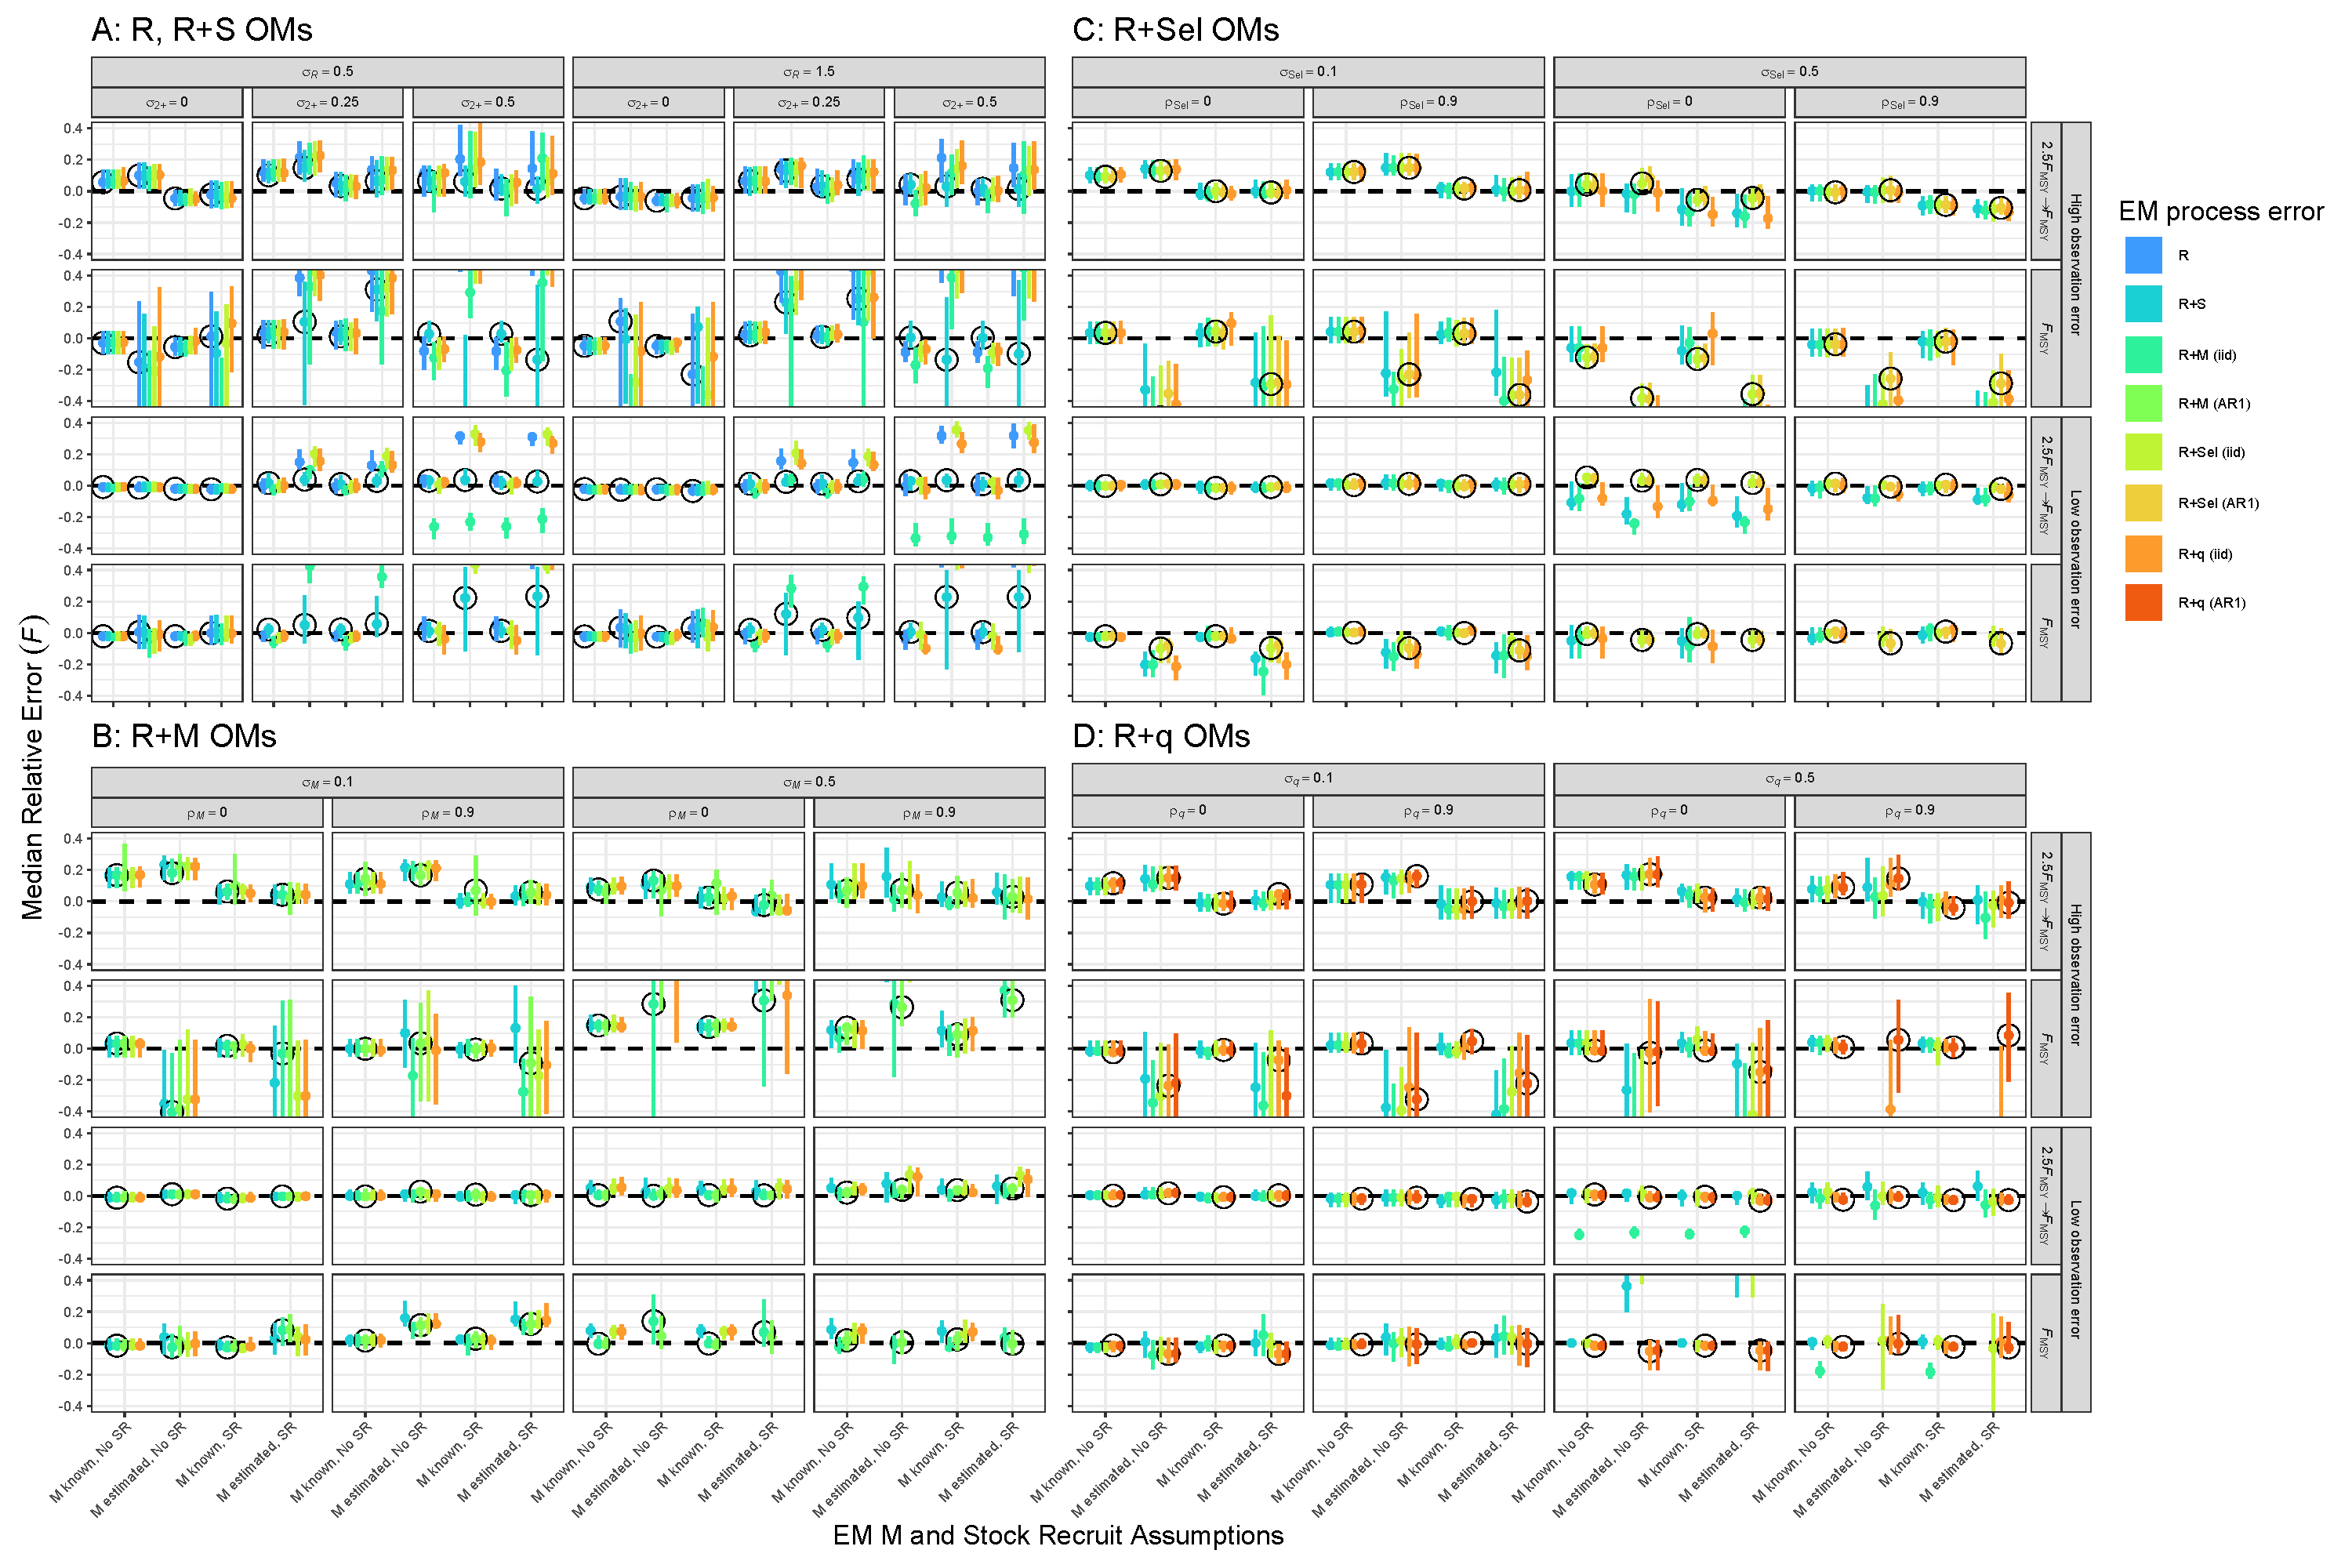
\includegraphics[width = 1.4\textwidth]{term_F_bias_plots}
\end{center}
\caption{\DIFaddFL{Median relative error of terminal year fully-selected fishing mortality for estimating models fitted to data sets simulated with alternative process error structures: R and R+S (A), R+Sel (B), R+M (C), or R+q (D). Circled values indicate results where the EM process error structure matches that of the operating model and vertical lines represent 95\% confidence intervals.}}\label{F_rel_error}
\end{figure}
\end{landscape}

\begin{landscape}
\begin{figure}
\begin{center}
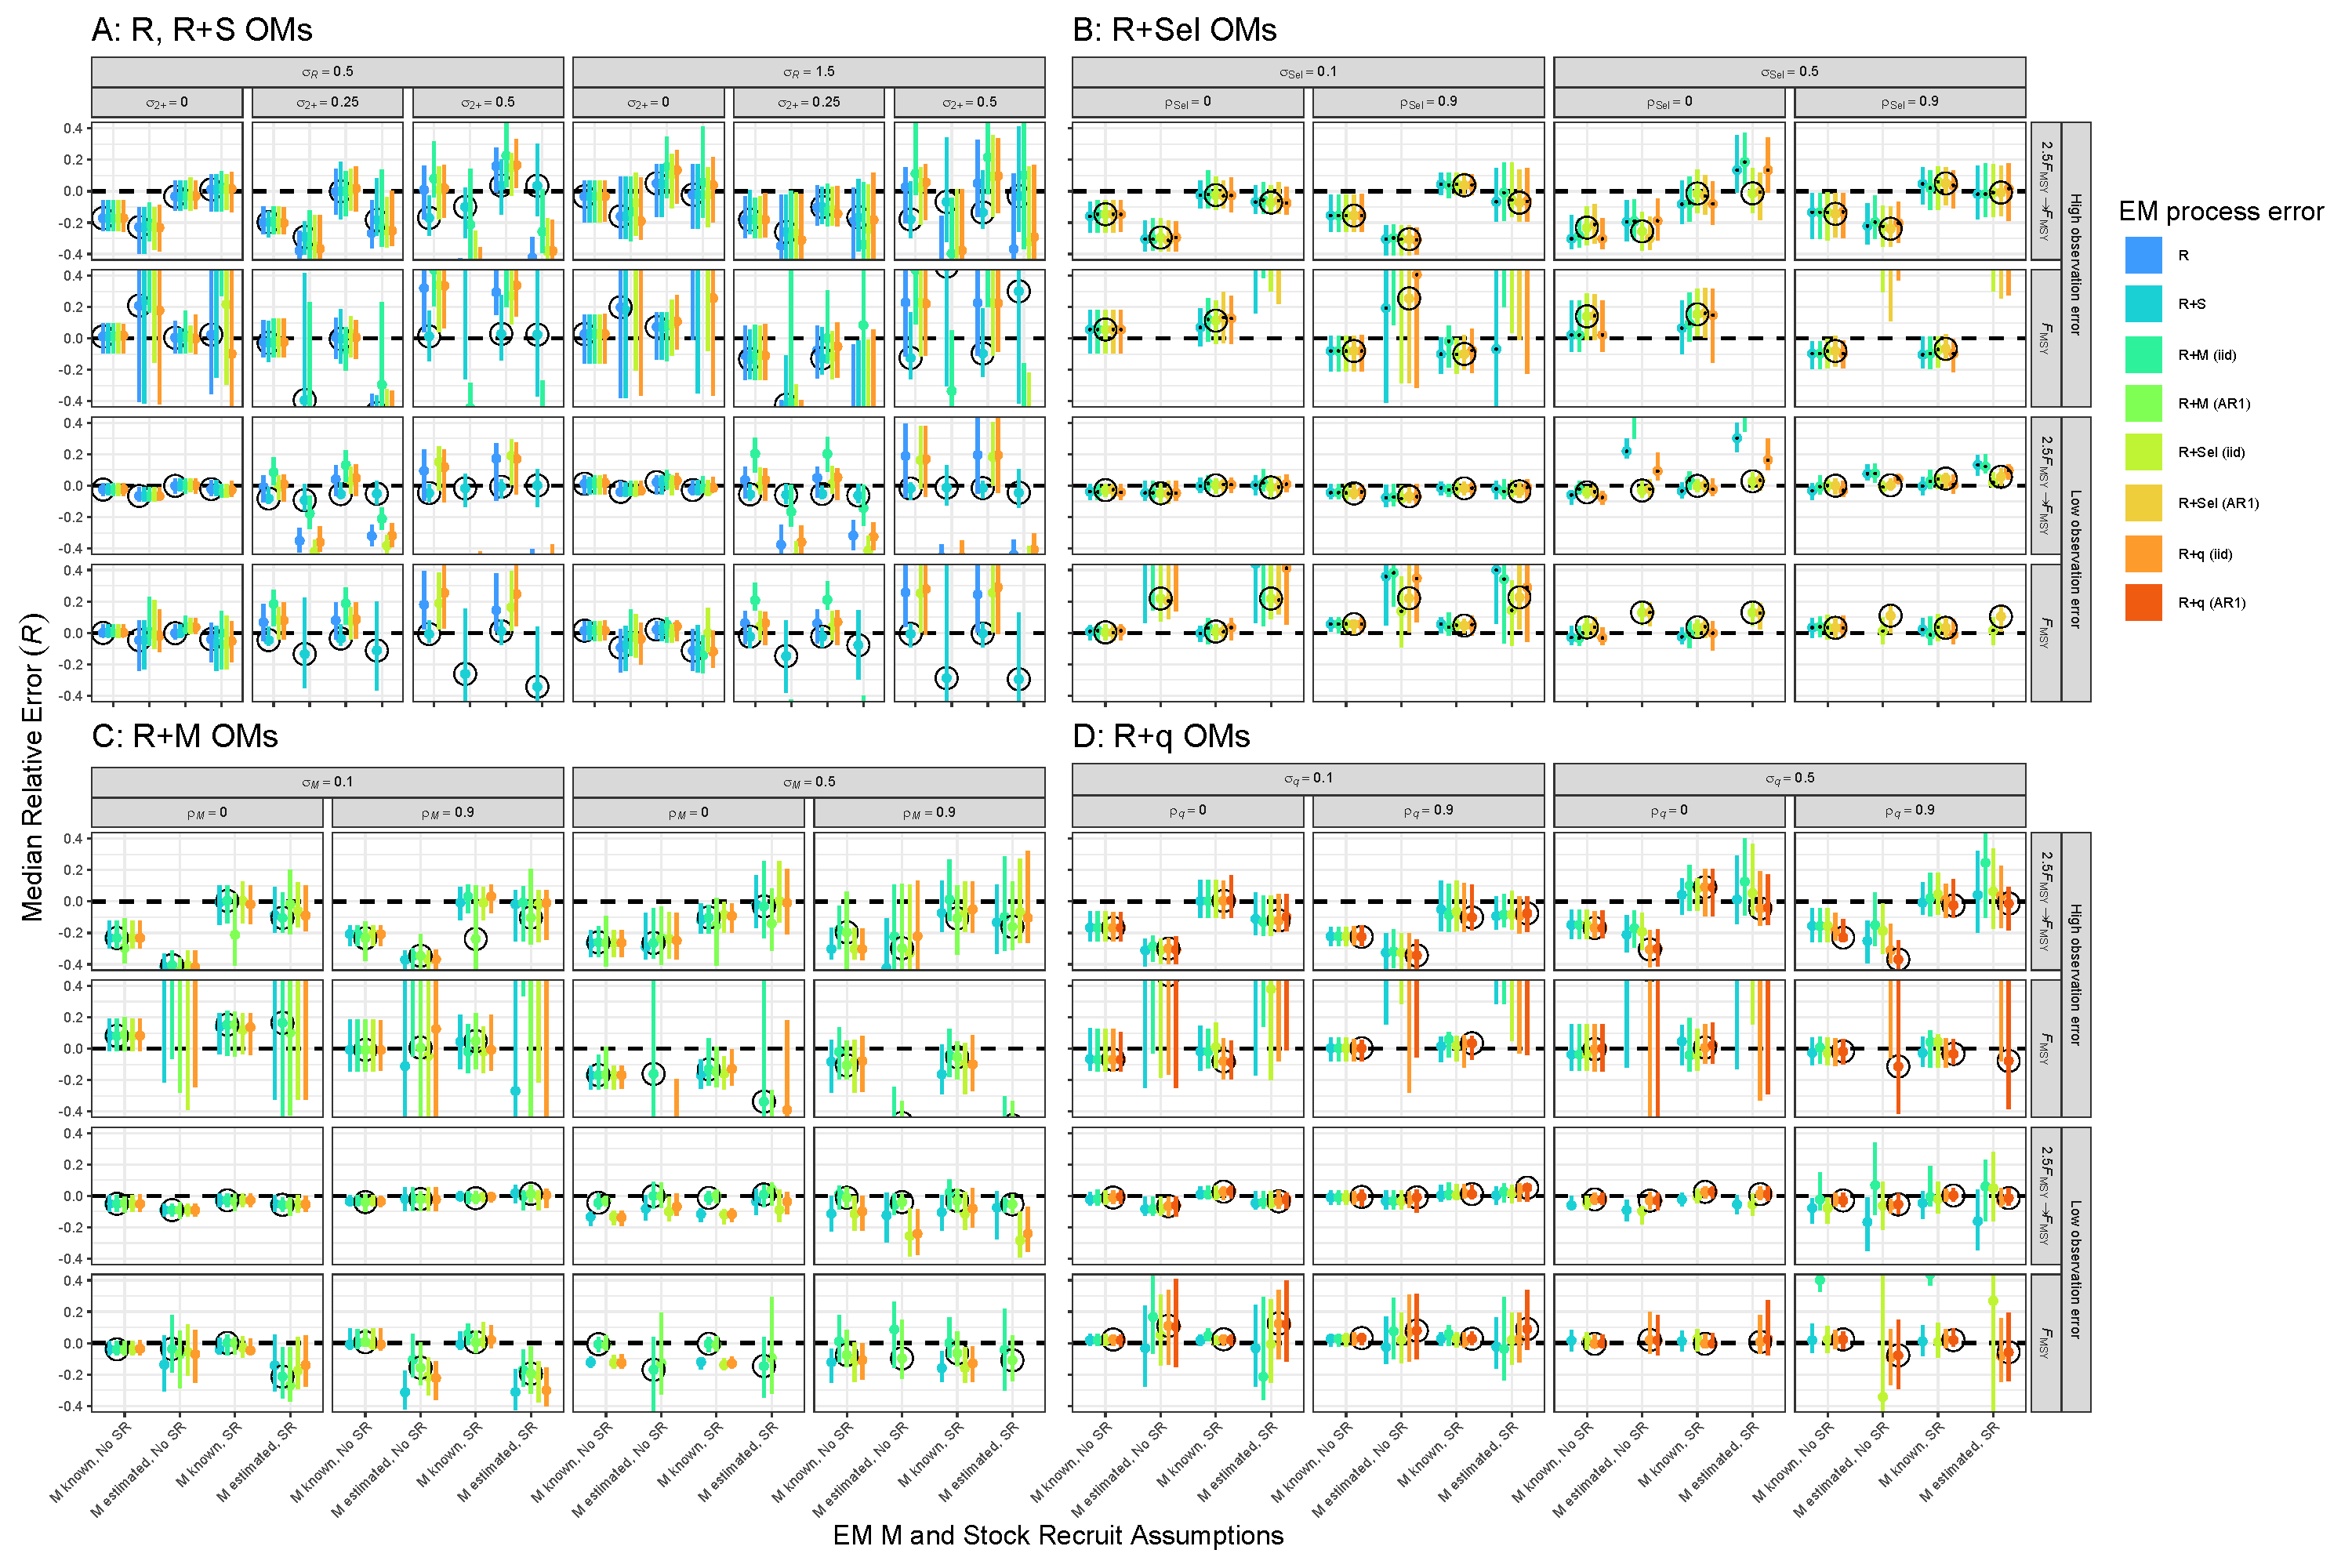
\includegraphics[width = 1.4\textwidth]{term_R_bias_plots}
\end{center}
\caption{\DIFaddFL{Median relative error of terminal year recruitment for estimating models fitted to data sets simulated with alternative process error structures: R and R+S (A), R+Sel (B), R+M (C), or R+q (D). Circled values indicate results where the EM process error structure matches that of the operating model and vertical lines represent 95\% confidence intervals.}}\label{R_rel_error}
\end{figure}
\end{landscape}

\begin{landscape}
\begin{figure}
\begin{center}
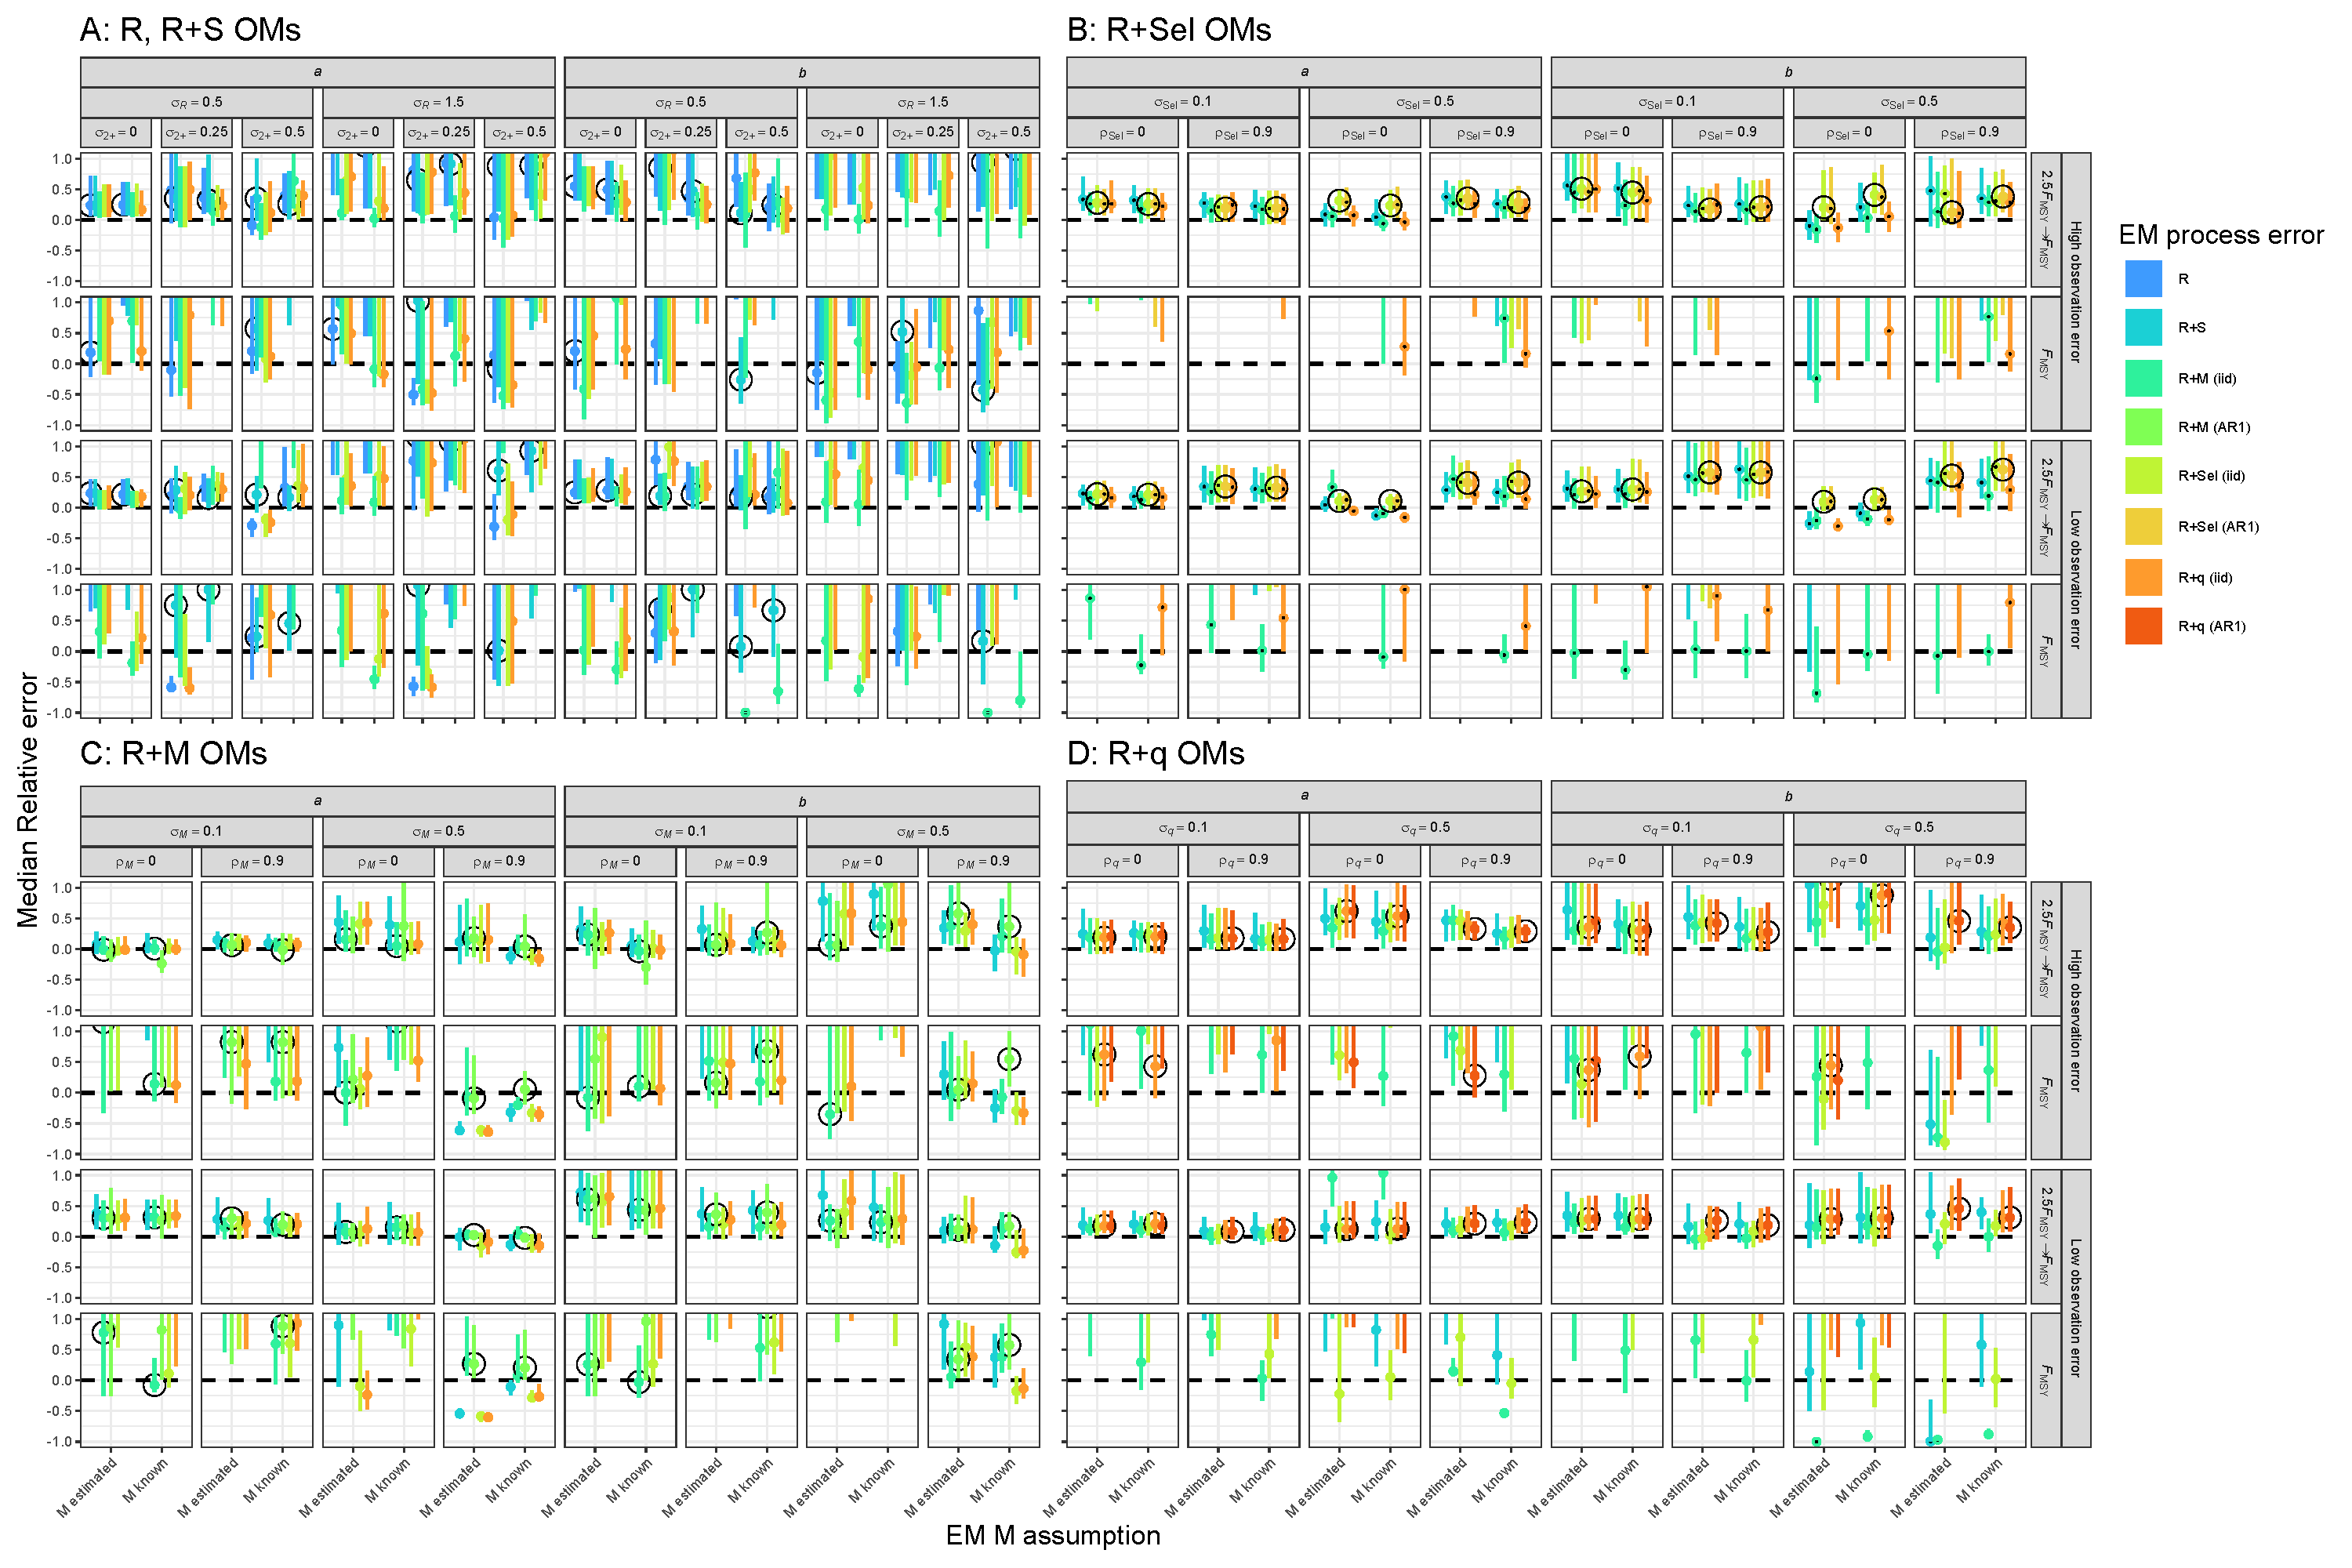
\includegraphics[width = 1.4\textwidth]{sr_bias_plots}
\end{center}
\caption{\DIFaddFL{Median relative error of Beverton-Holt stock-recruit parameters ($a$ and $b$) for estimating models fitted to data sets simulated with alternative process error structures: R and R+S (A), R+Sel (B), R+M (C), or R+q (D). Circled values indicate results where the EM process error structure matches that of the operating model and vertical lines represent 95\% confidence intervals.}}\label{SR_rel_error}
\end{figure}
\end{landscape}

\begin{landscape}
\begin{figure}
\begin{center}
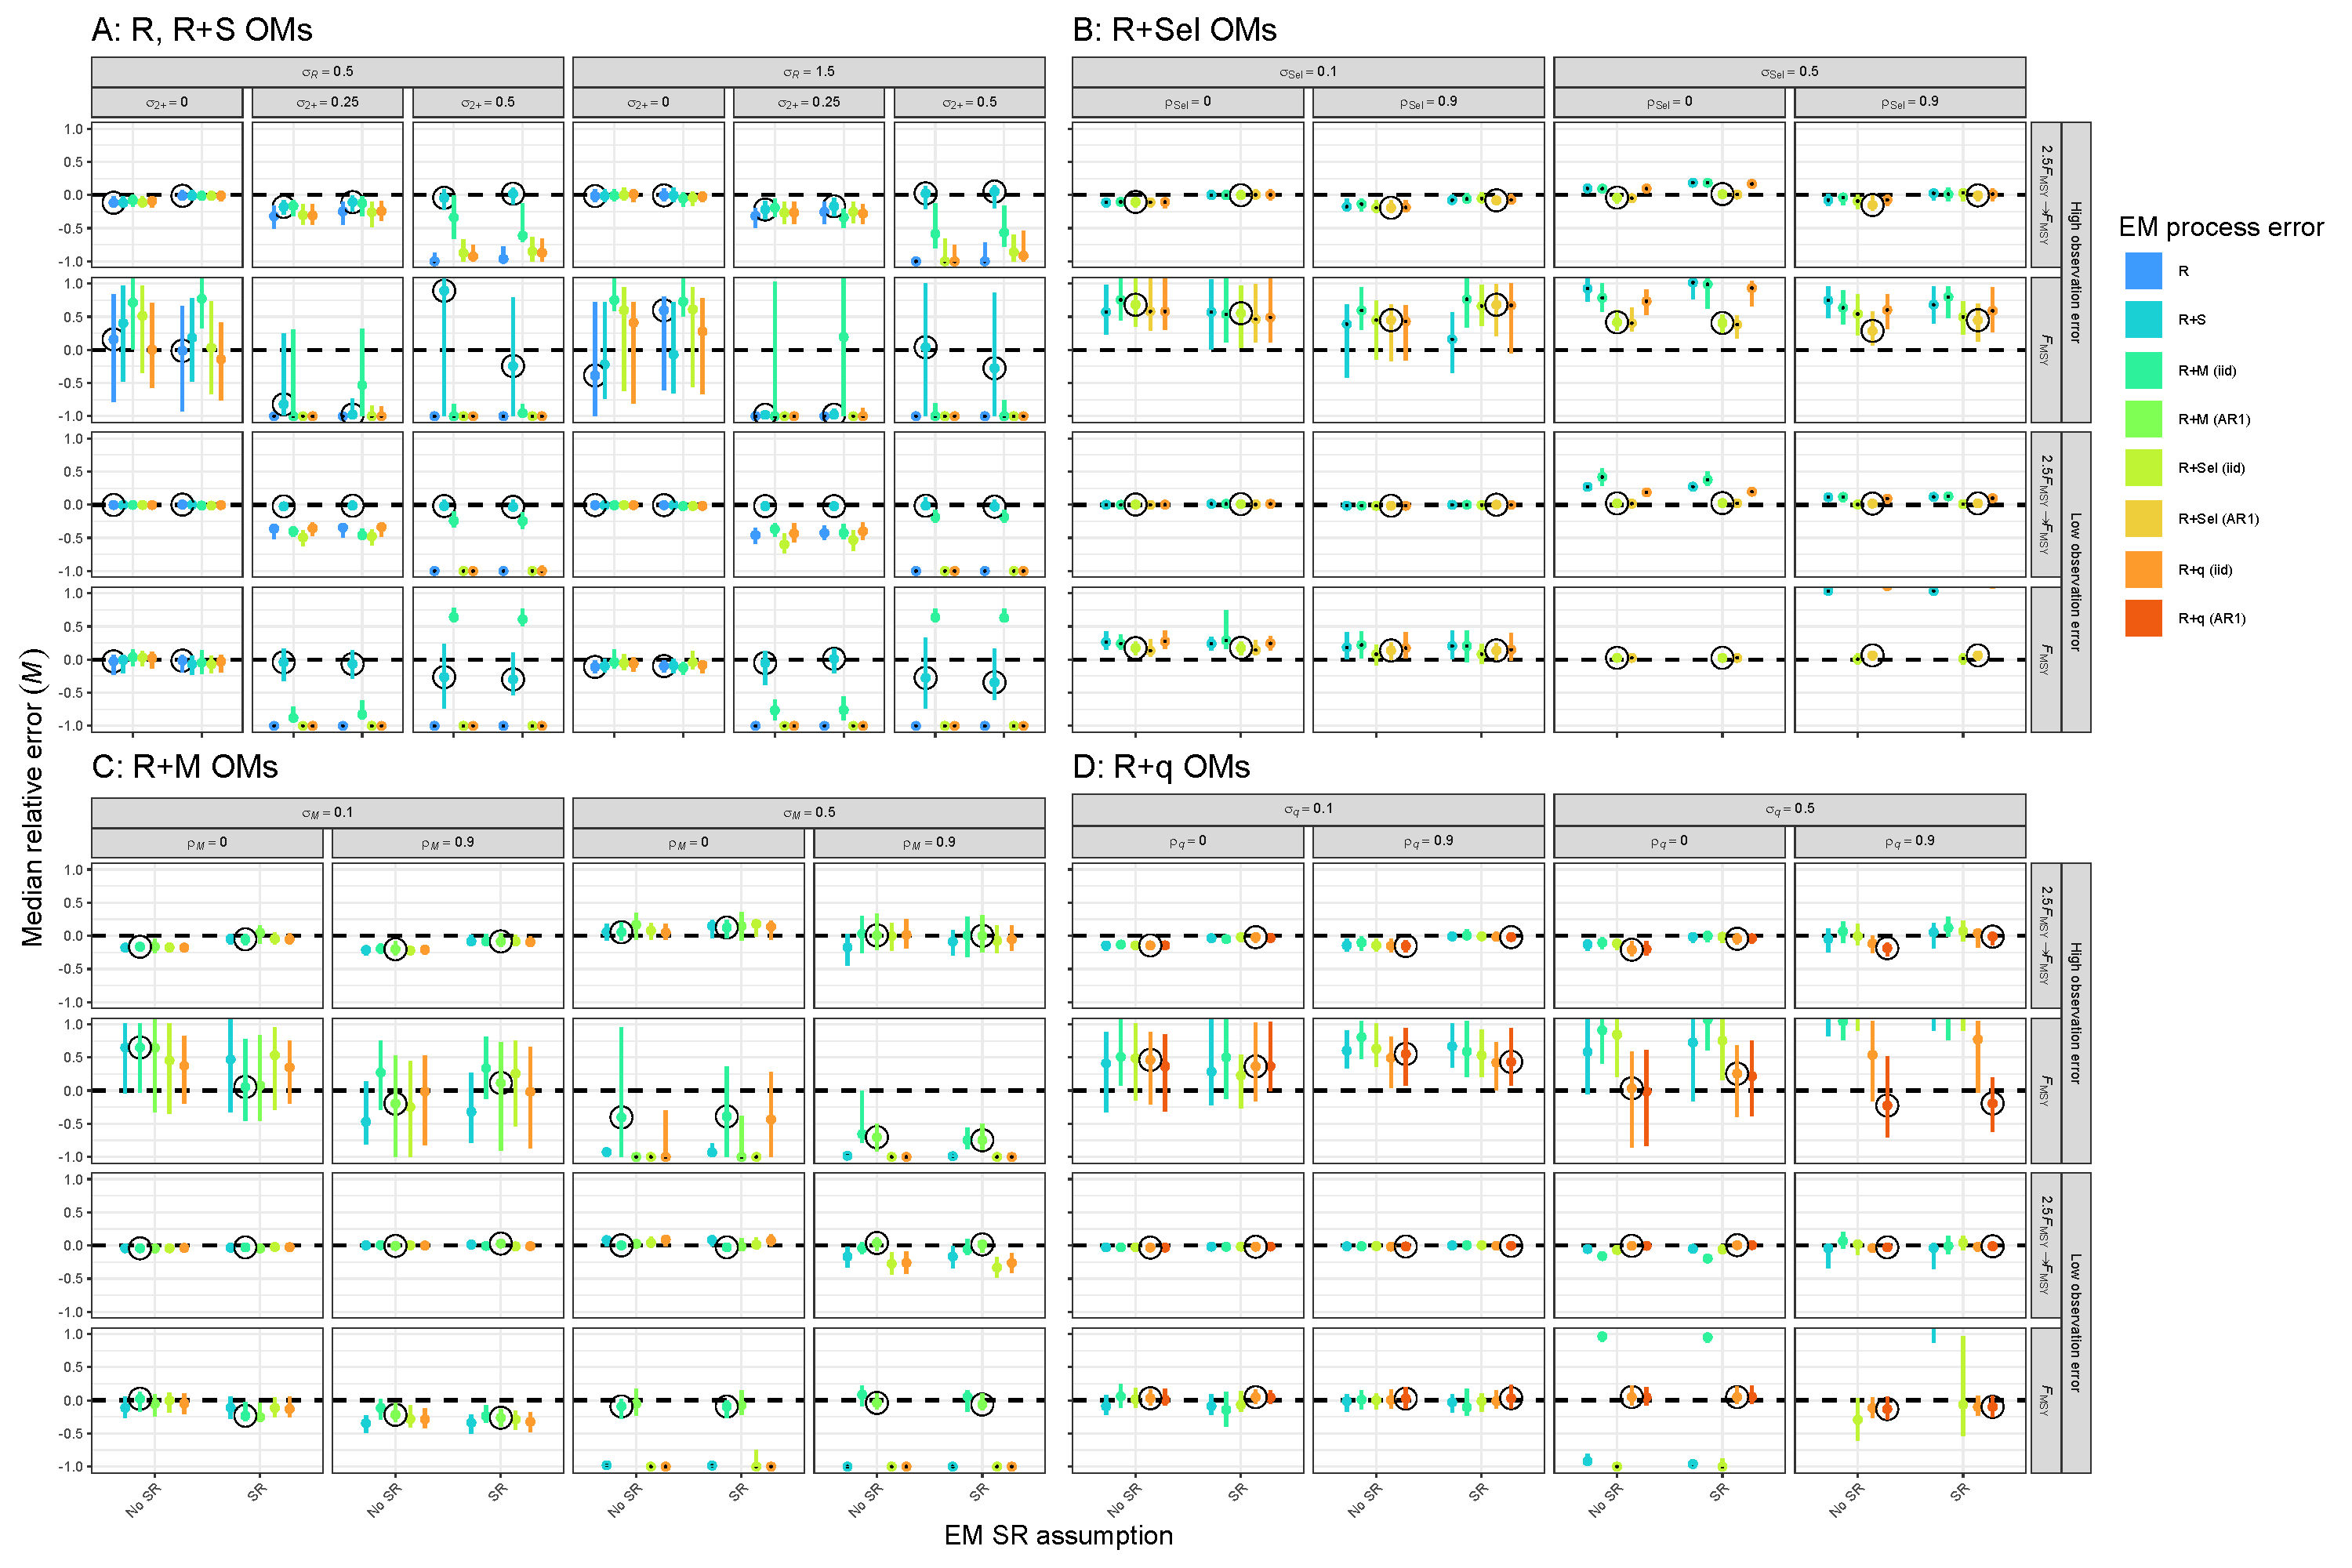
\includegraphics[width = 1.4\textwidth]{M_bias_plots}
\end{center}
\caption{\DIFaddFL{Median relative error of median natural mortality for estimating models fitted to data sets simulated with alternative process error structures: R and R+S (A), R+Sel (B), R+M (C), or R+q (D). Circled values indicate results where the EM process error structure matches that of the operating model and vertical lines represent 95\% confidence intervals.}}\label{M_rel_error}
\end{figure}
\end{landscape}

\begin{landscape}
\begin{figure}
\begin{center}
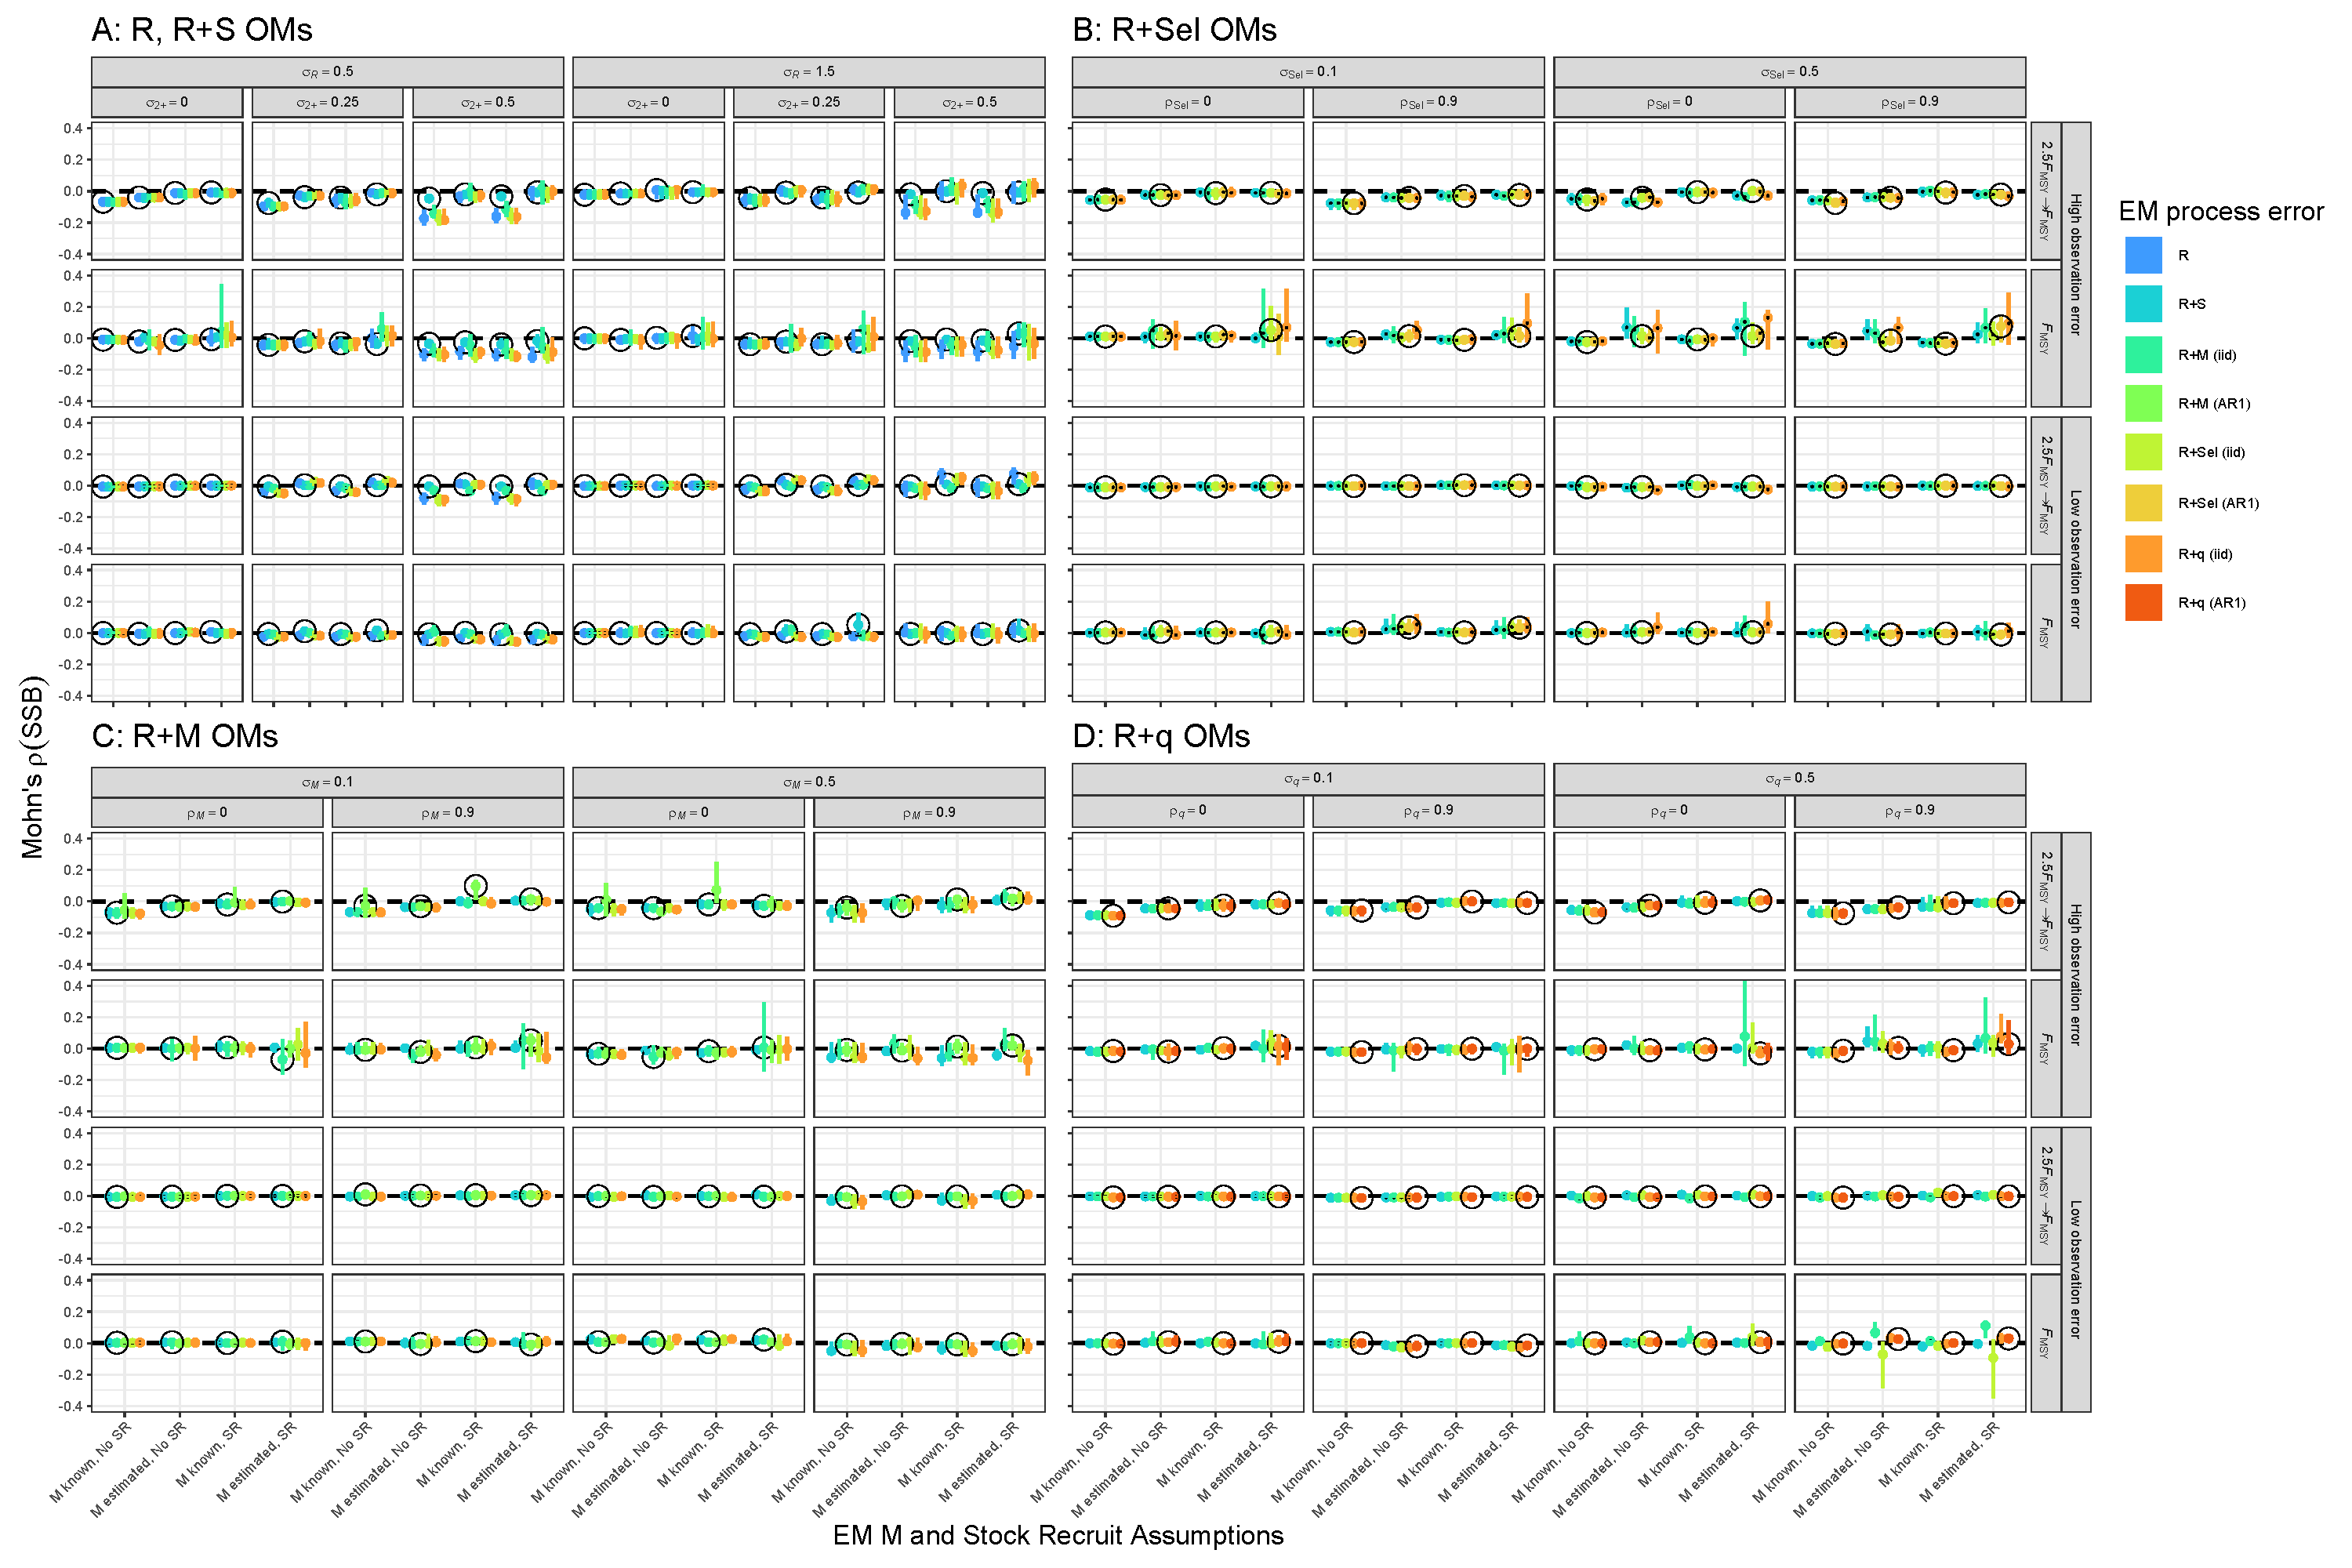
\includegraphics[width = 1.4\textwidth]{mohns_rho_ssb_plots}
\end{center}
\caption{\DIFaddFL{Median Mohn's $\rho$ for SSB for estimating models fitted to data sets simulated with alternative process error structures: R and R+S (A), R+Sel (B), R+M (C), or R+q (D). Circled values indicate results where the EM process error structure matches that of the operating model and vertical lines represent 95\% confidence intervals.}}\label{mohns_rho_ssb}
\end{figure}
\end{landscape}

\begin{landscape}
\begin{figure}
\begin{center}
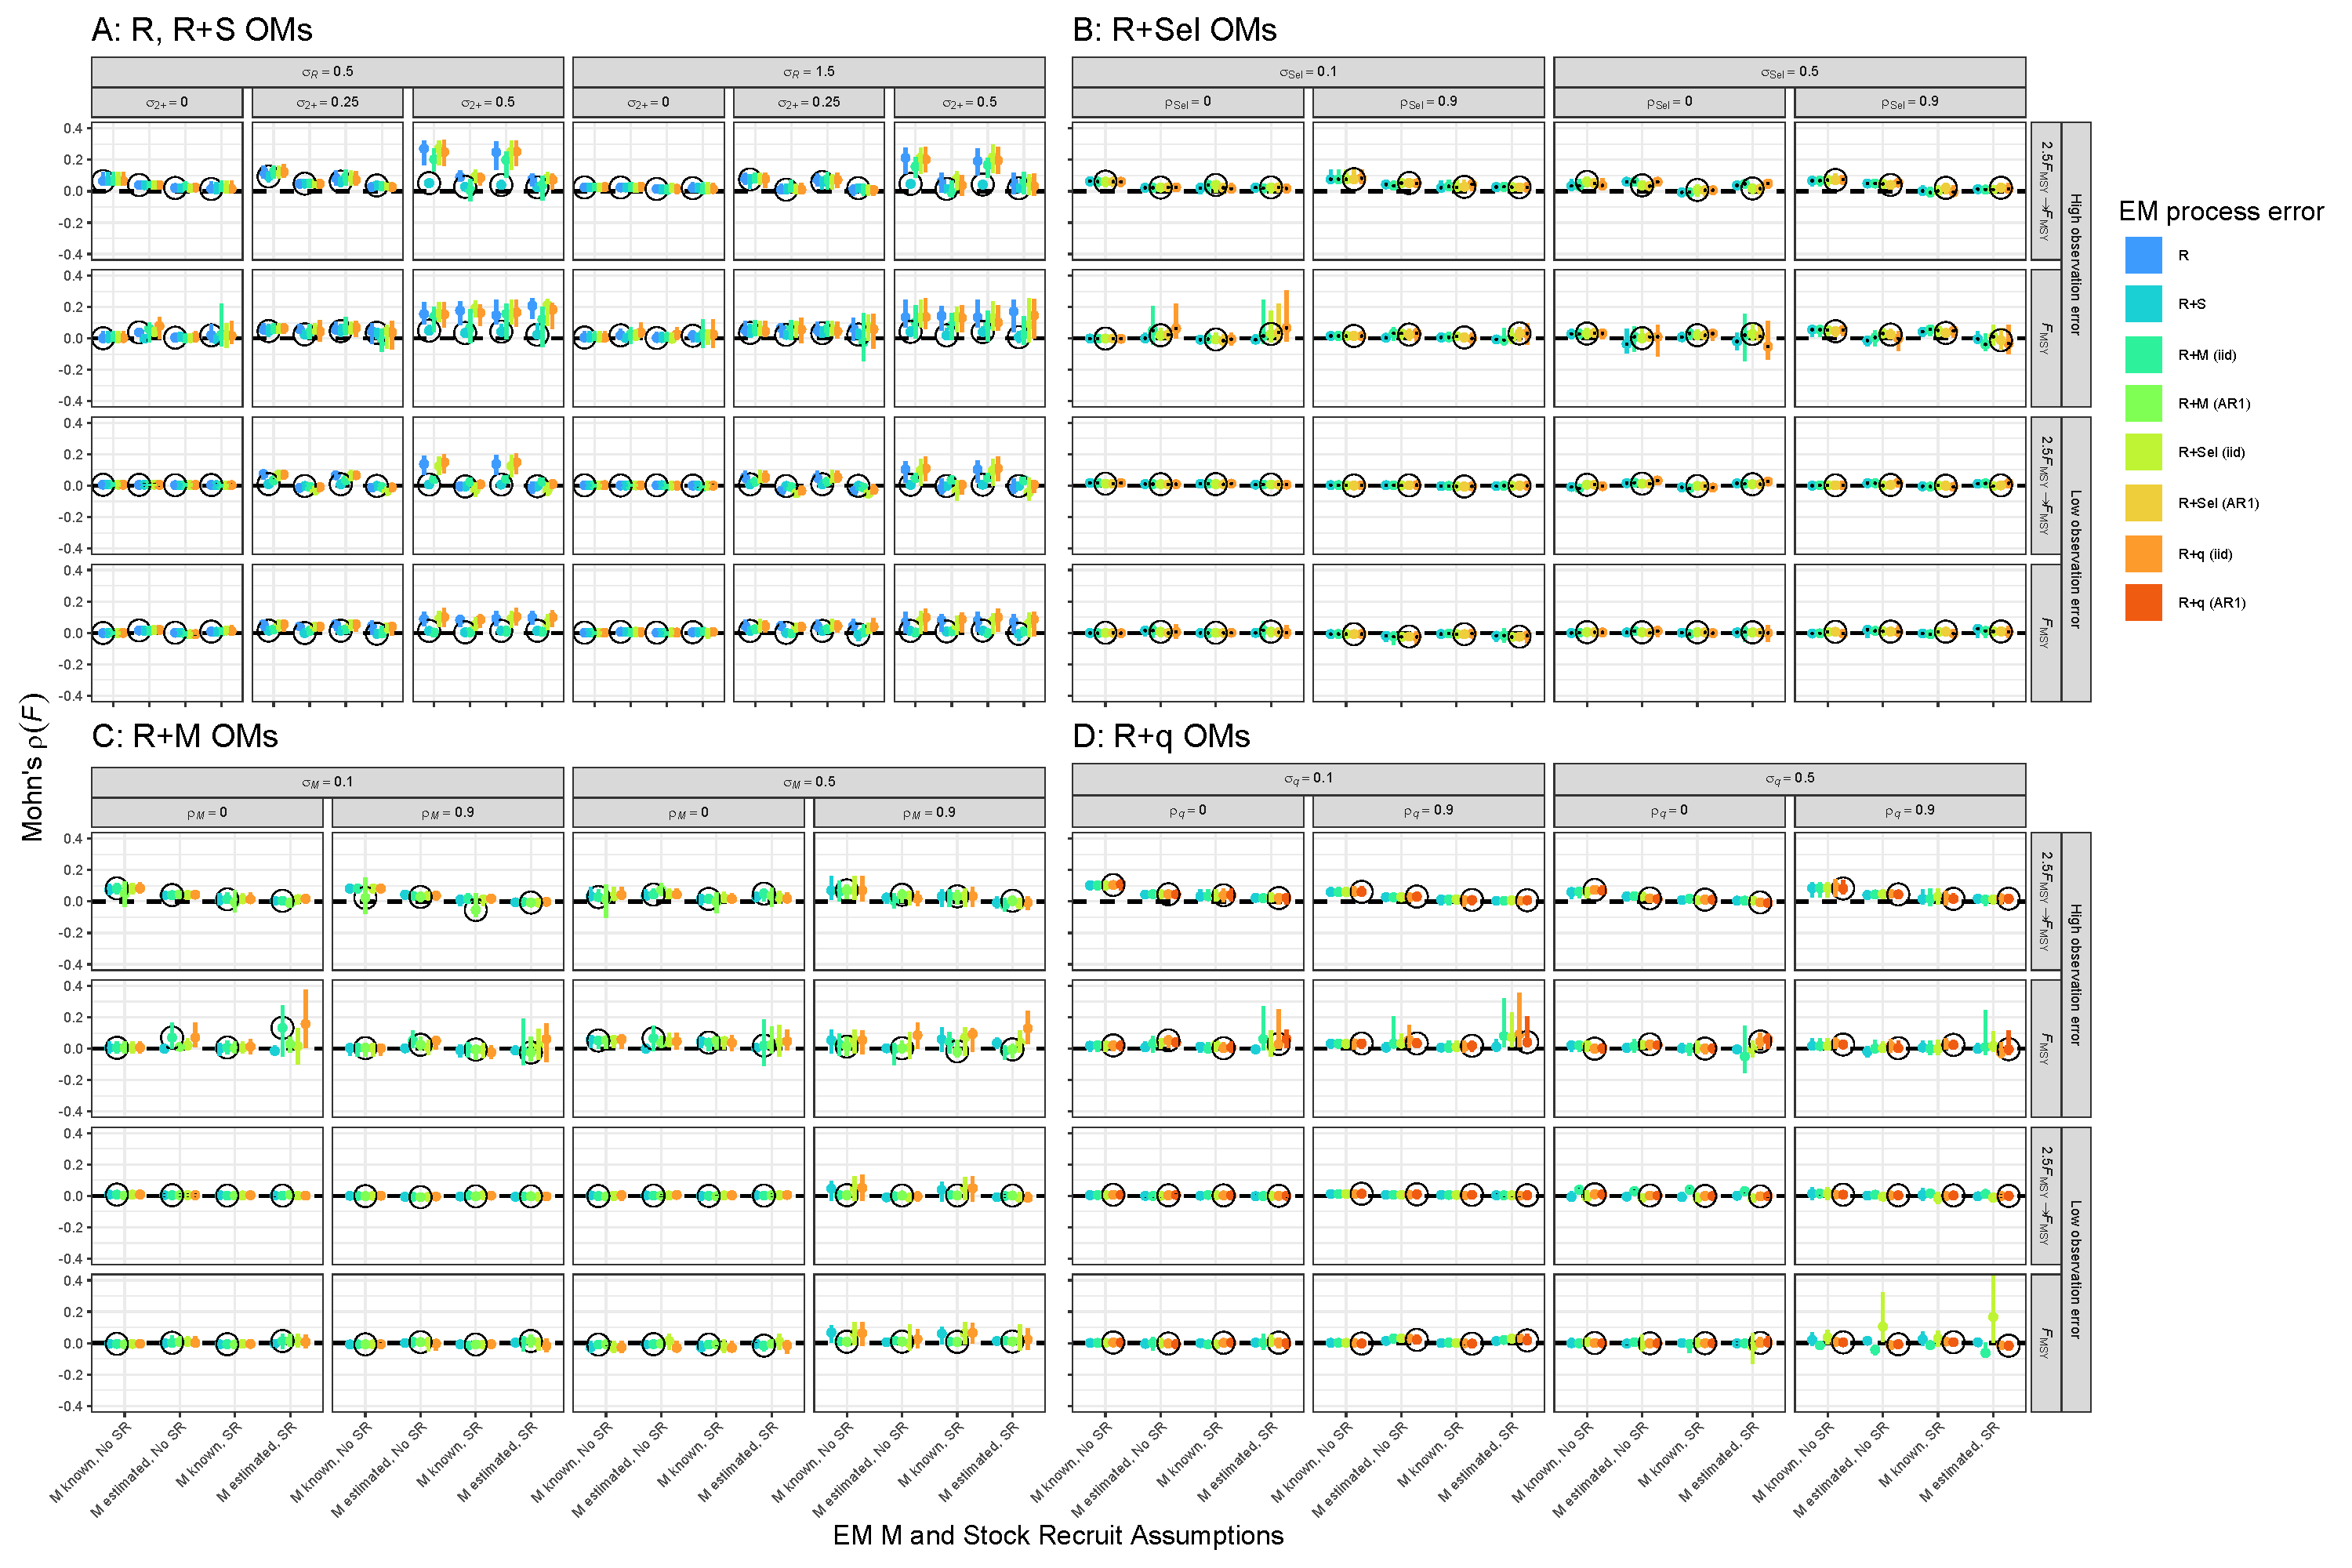
\includegraphics[width = 1.4\textwidth]{mohns_rho_F_plots}
\end{center}
\caption{\DIFaddFL{Median Mohn's $\rho$ of fishing mortality averaged over all age classes for estimating models fitted to data sets simulated with alternative process error structures: R and R+S (A), R+Sel (B), R+M (C), or R+q (D). Circled values indicate results where the EM process error structure matches that of the operating model and vertical lines represent 95\% confidence intervals.}}\label{mohns_rho_F}
\end{figure}
\end{landscape}

\begin{landscape}
\begin{figure}
\begin{center}
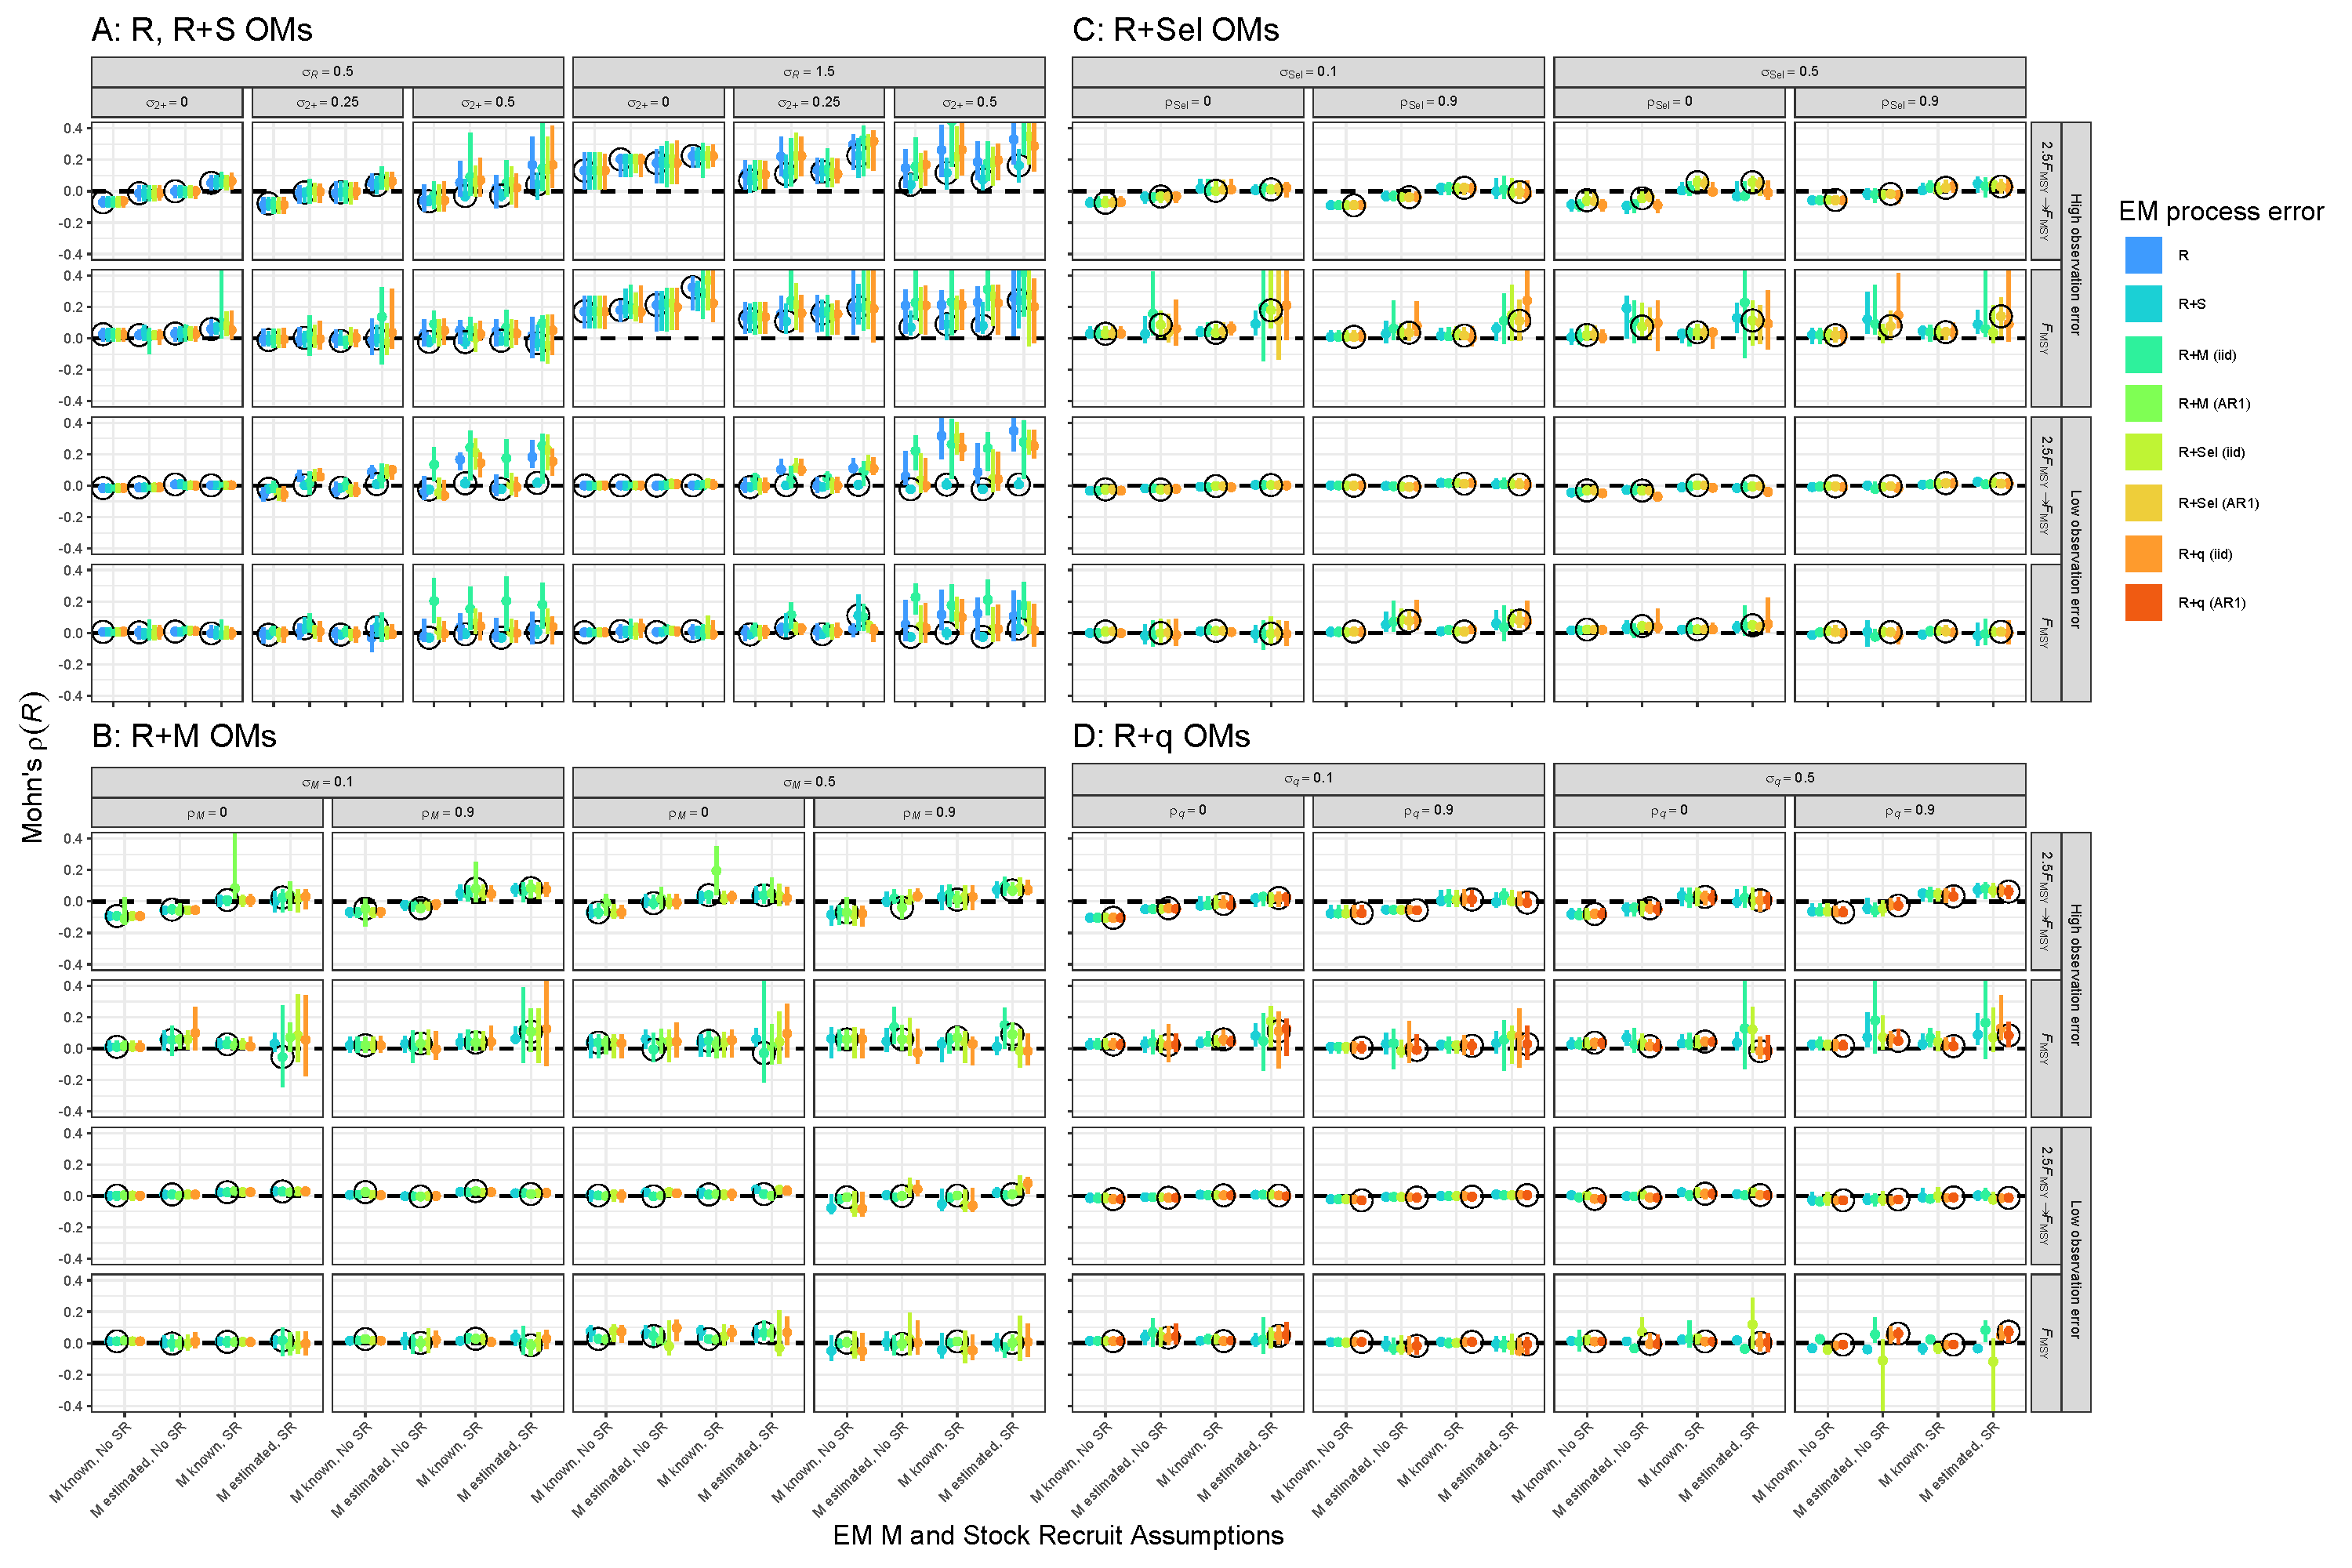
\includegraphics[width = 1.4\textwidth]{mohns_rho_R_plots}
\end{center}
\caption{\DIFaddFL{Median Mohn's $\rho$ of recruitment for estimating models fitted to data sets simulated with alternative process error structures: R and R+S (A), R+Sel (B), R+M (C), or R+q (D). Circled values indicate results where the EM process error structure matches that of the operating model and vertical lines represent 95\% confidence intervals.}}\label{mohns_rho_R}
\end{figure}
\end{landscape}

\begin{landscape}
\begin{table}
\DIFaddendFL \caption{Distinguishing characteristics of the operating models with random effects on recruitment and apparent survival (R.R+S). Standard deviations (SD) are for log-normal distributed indices and logistic normal distributed age composition observations (fleet and indices). Fishing mortality changes after year 20 (of 40) for fishing histories where fishing mortality is not constant.}\label{naa_om_table}
{\footnotesize \begin{center}
\begin{tabular}{rrrrr}
\hline\hline
\multicolumn{1}{c}{Model}&\multicolumn{1}{c}{$\sigma_R$}&\multicolumn{1}{c}{$\sigma_{2+}$}&\multicolumn{1}{c}{Fishing History}&\multicolumn{1}{c}{Observation Uncertainty}\tabularnewline
\hline
$\text{NAA}_{1}$&$0.5$&$$&$2.5 F_{\text{MSY}} \rightarrow F_{\text{MSY}}$&Index SD = 0.1, Age composition SD = 0.3\tabularnewline
$\text{NAA}_{2}$&$1.5$&$$&$2.5 F_{\text{MSY}} \rightarrow F_{\text{MSY}}$&Index SD = 0.1, Age composition SD = 0.3\tabularnewline
$\text{NAA}_{3}$&$0.5$&$0.25$&$2.5 F_{\text{MSY}} \rightarrow F_{\text{MSY}}$&Index SD = 0.1, Age composition SD = 0.3\tabularnewline
$\text{NAA}_{4}$&$1.5$&$0.25$&$2.5 F_{\text{MSY}} \rightarrow F_{\text{MSY}}$&Index SD = 0.1, Age composition SD = 0.3\tabularnewline
$\text{NAA}_{5}$&$0.5$&$0.50$&$2.5 F_{\text{MSY}} \rightarrow F_{\text{MSY}}$&Index SD = 0.1, Age composition SD = 0.3\tabularnewline
$\text{NAA}_{6}$&$1.5$&$0.50$&$2.5 F_{\text{MSY}} \rightarrow F_{\text{MSY}}$&Index SD = 0.1, Age composition SD = 0.3\tabularnewline
$\text{NAA}_{7}$&$0.5$&$$&$F_{\text{MSY}}$&Index SD = 0.1, Age composition SD = 0.3\tabularnewline
$\text{NAA}_{8}$&$1.5$&$$&$F_{\text{MSY}}$&Index SD = 0.1, Age composition SD = 0.3\tabularnewline
$\text{NAA}_{9}$&$0.5$&$0.25$&$F_{\text{MSY}}$&Index SD = 0.1, Age composition SD = 0.3\tabularnewline
$\text{NAA}_{10}$&$1.5$&$0.25$&$F_{\text{MSY}}$&Index SD = 0.1, Age composition SD = 0.3\tabularnewline
$\text{NAA}_{11}$&$0.5$&$0.50$&$F_{\text{MSY}}$&Index SD = 0.1, Age composition SD = 0.3\tabularnewline
$\text{NAA}_{12}$&$1.5$&$0.50$&$F_{\text{MSY}}$&Index SD = 0.1, Age composition SD = 0.3\tabularnewline
$\text{NAA}_{13}$&$0.5$&$$&$2.5 F_{\text{MSY}} \rightarrow F_{\text{MSY}}$&Index SD = 0.4, Age composition SD = 1.5\tabularnewline
$\text{NAA}_{14}$&$1.5$&$$&$2.5 F_{\text{MSY}} \rightarrow F_{\text{MSY}}$&Index SD = 0.4, Age composition SD = 1.5\tabularnewline
$\text{NAA}_{15}$&$0.5$&$0.25$&$2.5 F_{\text{MSY}} \rightarrow F_{\text{MSY}}$&Index SD = 0.4, Age composition SD = 1.5\tabularnewline
$\text{NAA}_{16}$&$1.5$&$0.25$&$2.5 F_{\text{MSY}} \rightarrow F_{\text{MSY}}$&Index SD = 0.4, Age composition SD = 1.5\tabularnewline
$\text{NAA}_{17}$&$0.5$&$0.50$&$2.5 F_{\text{MSY}} \rightarrow F_{\text{MSY}}$&Index SD = 0.4, Age composition SD = 1.5\tabularnewline
$\text{NAA}_{18}$&$1.5$&$0.50$&$2.5 F_{\text{MSY}} \rightarrow F_{\text{MSY}}$&Index SD = 0.4, Age composition SD = 1.5\tabularnewline
$\text{NAA}_{19}$&$0.5$&$$&$F_{\text{MSY}}$&Index SD = 0.4, Age composition SD = 1.5\tabularnewline
$\text{NAA}_{20}$&$1.5$&$$&$F_{\text{MSY}}$&Index SD = 0.4, Age composition SD = 1.5\tabularnewline
$\text{NAA}_{21}$&$0.5$&$0.25$&$F_{\text{MSY}}$&Index SD = 0.4, Age composition SD = 1.5\tabularnewline
$\text{NAA}_{22}$&$1.5$&$0.25$&$F_{\text{MSY}}$&Index SD = 0.4, Age composition SD = 1.5\tabularnewline
$\text{NAA}_{23}$&$0.5$&$0.50$&$F_{\text{MSY}}$&Index SD = 0.4, Age composition SD = 1.5\tabularnewline
$\text{NAA}_{24}$&$1.5$&$0.50$&$F_{\text{MSY}}$&Index SD = 0.4, Age composition SD = 1.5\tabularnewline
\hline
\end{tabular}\end{center}
}
\end{table}
\end{landscape}

\begin{landscape}
\begin{table}
\caption{Distinguishing characteristics of the operating models with random effects on recruitment and natural mortality (R+M). Standard deviations (SD) are for log-normal distributed indices and logistic normal distributed age composition observations (fleet and indices). Fishing mortality changes after year 20 (of 40) for fishing histories where fishing mortality is not constant. For AR1 process errors, $\sigma$ is defined for the marginal distribution of the processes.}\label{M_om_table}
{\begin{center}
\begin{tabular}{rrrrrr}
\hline\hline
\multicolumn{1}{c}{Model}&\multicolumn{1}{c}{$\sigma_R$}&\multicolumn{1}{c}{$\sigma_{M}$}&\multicolumn{1}{c}{$\rho_{M}$}&\multicolumn{1}{c}{Fishing History}&\multicolumn{1}{c}{Observation Uncertainty}\tabularnewline
\hline
$M_{1}$&$0.5$&$0.1$&$0.0$&$2.5 F_{\text{MSY}} \rightarrow F_{\text{MSY}}$&Index SD = 0.1, Age composition SD = 0.3\tabularnewline
$M_{2}$&$0.5$&$0.5$&$0.0$&$2.5 F_{\text{MSY}} \rightarrow F_{\text{MSY}}$&Index SD = 0.1, Age composition SD = 0.3\tabularnewline
$M_{3}$&$0.5$&$0.1$&$0.9$&$2.5 F_{\text{MSY}} \rightarrow F_{\text{MSY}}$&Index SD = 0.1, Age composition SD = 0.3\tabularnewline
$M_{4}$&$0.5$&$0.5$&$0.9$&$2.5 F_{\text{MSY}} \rightarrow F_{\text{MSY}}$&Index SD = 0.1, Age composition SD = 0.3\tabularnewline
$M_{5}$&$0.5$&$0.1$&$0.0$&$F_{\text{MSY}}$&Index SD = 0.1, Age composition SD = 0.3\tabularnewline
$M_{6}$&$0.5$&$0.5$&$0.0$&$F_{\text{MSY}}$&Index SD = 0.1, Age composition SD = 0.3\tabularnewline
$M_{7}$&$0.5$&$0.1$&$0.9$&$F_{\text{MSY}}$&Index SD = 0.1, Age composition SD = 0.3\tabularnewline
$M_{8}$&$0.5$&$0.5$&$0.9$&$F_{\text{MSY}}$&Index SD = 0.1, Age composition SD = 0.3\tabularnewline
$M_{9}$&$0.5$&$0.1$&$0.0$&$2.5 F_{\text{MSY}} \rightarrow F_{\text{MSY}}$&Index SD = 0.4, Age composition SD = 1.5\tabularnewline
$M_{10}$&$0.5$&$0.5$&$0.0$&$2.5 F_{\text{MSY}} \rightarrow F_{\text{MSY}}$&Index SD = 0.4, Age composition SD = 1.5\tabularnewline
$M_{11}$&$0.5$&$0.1$&$0.9$&$2.5 F_{\text{MSY}} \rightarrow F_{\text{MSY}}$&Index SD = 0.4, Age composition SD = 1.5\tabularnewline
$M_{12}$&$0.5$&$0.5$&$0.9$&$2.5 F_{\text{MSY}} \rightarrow F_{\text{MSY}}$&Index SD = 0.4, Age composition SD = 1.5\tabularnewline
$M_{13}$&$0.5$&$0.1$&$0.0$&$F_{\text{MSY}}$&Index SD = 0.4, Age composition SD = 1.5\tabularnewline
$M_{14}$&$0.5$&$0.5$&$0.0$&$F_{\text{MSY}}$&Index SD = 0.4, Age composition SD = 1.5\tabularnewline
$M_{15}$&$0.5$&$0.1$&$0.9$&$F_{\text{MSY}}$&Index SD = 0.4, Age composition SD = 1.5\tabularnewline
$M_{16}$&$0.5$&$0.5$&$0.9$&$F_{\text{MSY}}$&Index SD = 0.4, Age composition SD = 1.5\tabularnewline
\hline
\end{tabular}\end{center}
}
\end{table}
\end{landscape}

\begin{landscape}
\begin{table}
\caption{Distinguishing characteristics of the operating models with random effects on recruitment and selectivity (R+Sel). Standard deviations (SD) are for log-normal distributed indices and logistic normal distributed age composition observations (fleet and indices). Fishing mortality changes after year 20 (of 40) for fishing histories where fishing mortality is not constant. For AR1 process errors, $\sigma$ is defined for the marginal distribution of the processes.}\label{sel_om_table}
{\begin{center}
\begin{tabular}{rrrrrr}
\hline\hline
\multicolumn{1}{c}{Model}&\multicolumn{1}{c}{$\sigma_R$}&\multicolumn{1}{c}{$\sigma_{\text{Sel}}$}&\multicolumn{1}{c}{$\rho_{\text{Sel}}$}&\multicolumn{1}{c}{Fishing History}&\multicolumn{1}{c}{Observation Uncertainty}\tabularnewline
\hline
$\text{Sel}_{1}$&$0.5$&$0.1$&$0.0$&$2.5 F_{\text{MSY}} \rightarrow F_{\text{MSY}}$&Index SD = 0.1, Age composition SD = 0.3\tabularnewline
$\text{Sel}_{2}$&$0.5$&$0.5$&$0.0$&$2.5 F_{\text{MSY}} \rightarrow F_{\text{MSY}}$&Index SD = 0.1, Age composition SD = 0.3\tabularnewline
$\text{Sel}_{3}$&$0.5$&$0.1$&$0.9$&$2.5 F_{\text{MSY}} \rightarrow F_{\text{MSY}}$&Index SD = 0.1, Age composition SD = 0.3\tabularnewline
$\text{Sel}_{4}$&$0.5$&$0.5$&$0.9$&$2.5 F_{\text{MSY}} \rightarrow F_{\text{MSY}}$&Index SD = 0.1, Age composition SD = 0.3\tabularnewline
$\text{Sel}_{5}$&$0.5$&$0.1$&$0.0$&$F_{\text{MSY}}$&Index SD = 0.1, Age composition SD = 0.3\tabularnewline
$\text{Sel}_{6}$&$0.5$&$0.5$&$0.0$&$F_{\text{MSY}}$&Index SD = 0.1, Age composition SD = 0.3\tabularnewline
$\text{Sel}_{7}$&$0.5$&$0.1$&$0.9$&$F_{\text{MSY}}$&Index SD = 0.1, Age composition SD = 0.3\tabularnewline
$\text{Sel}_{8}$&$0.5$&$0.5$&$0.9$&$F_{\text{MSY}}$&Index SD = 0.1, Age composition SD = 0.3\tabularnewline
$\text{Sel}_{9}$&$0.5$&$0.1$&$0.0$&$2.5 F_{\text{MSY}} \rightarrow F_{\text{MSY}}$&Index SD = 0.4, Age composition SD = 1.5\tabularnewline
$\text{Sel}_{10}$&$0.5$&$0.5$&$0.0$&$2.5 F_{\text{MSY}} \rightarrow F_{\text{MSY}}$&Index SD = 0.4, Age composition SD = 1.5\tabularnewline
$\text{Sel}_{11}$&$0.5$&$0.1$&$0.9$&$2.5 F_{\text{MSY}} \rightarrow F_{\text{MSY}}$&Index SD = 0.4, Age composition SD = 1.5\tabularnewline
$\text{Sel}_{12}$&$0.5$&$0.5$&$0.9$&$2.5 F_{\text{MSY}} \rightarrow F_{\text{MSY}}$&Index SD = 0.4, Age composition SD = 1.5\tabularnewline
$\text{Sel}_{13}$&$0.5$&$0.1$&$0.0$&$F_{\text{MSY}}$&Index SD = 0.4, Age composition SD = 1.5\tabularnewline
$\text{Sel}_{14}$&$0.5$&$0.5$&$0.0$&$F_{\text{MSY}}$&Index SD = 0.4, Age composition SD = 1.5\tabularnewline
$\text{Sel}_{15}$&$0.5$&$0.1$&$0.9$&$F_{\text{MSY}}$&Index SD = 0.4, Age composition SD = 1.5\tabularnewline
$\text{Sel}_{16}$&$0.5$&$0.5$&$0.9$&$F_{\text{MSY}}$&Index SD = 0.4, Age composition SD = 1.5\tabularnewline
\hline
\end{tabular}\end{center}
}
\end{table}
\end{landscape}

\begin{landscape}
\begin{table}
\caption{Distinguishing characteristics of the operating models with random effects on recruitment and catchability (R+q). Standard deviations (SD) are for log-normal distributed indices and logistic normal distributed age composition observations (fleet and indices). Fishing mortality changes after year 20 (of 40) for fishing histories where fishing mortality is not constant. For AR1 process errors, $\sigma$ is defined for the marginal distribution of the processes.}\label{q_om_table}
{\begin{center}
\begin{tabular}{rrrrrr}
\hline\hline
\multicolumn{1}{c}{Model}&\multicolumn{1}{c}{$\sigma_R$}&\multicolumn{1}{c}{$\sigma_{q}$}&\multicolumn{1}{c}{$\rho_{q}$}&\multicolumn{1}{c}{Fishing History}&\multicolumn{1}{c}{Observation Uncertainty}\tabularnewline
\hline
$q_{1}$&$0.5$&$0.1$&$0.0$&$2.5 F_{\text{MSY}} \rightarrow F_{\text{MSY}}$&Index SD = 0.1, Age composition SD = 0.3\tabularnewline
$q_{2}$&$0.5$&$0.5$&$0.0$&$2.5 F_{\text{MSY}} \rightarrow F_{\text{MSY}}$&Index SD = 0.1, Age composition SD = 0.3\tabularnewline
$q_{3}$&$0.5$&$0.1$&$0.9$&$2.5 F_{\text{MSY}} \rightarrow F_{\text{MSY}}$&Index SD = 0.1, Age composition SD = 0.3\tabularnewline
$q_{4}$&$0.5$&$0.5$&$0.9$&$2.5 F_{\text{MSY}} \rightarrow F_{\text{MSY}}$&Index SD = 0.1, Age composition SD = 0.3\tabularnewline
$q_{5}$&$0.5$&$0.1$&$0.0$&$F_{\text{MSY}}$&Index SD = 0.1, Age composition SD = 0.3\tabularnewline
$q_{6}$&$0.5$&$0.5$&$0.0$&$F_{\text{MSY}}$&Index SD = 0.1, Age composition SD = 0.3\tabularnewline
$q_{7}$&$0.5$&$0.1$&$0.9$&$F_{\text{MSY}}$&Index SD = 0.1, Age composition SD = 0.3\tabularnewline
$q_{8}$&$0.5$&$0.5$&$0.9$&$F_{\text{MSY}}$&Index SD = 0.1, Age composition SD = 0.3\tabularnewline
$q_{9}$&$0.5$&$0.1$&$0.0$&$2.5 F_{\text{MSY}} \rightarrow F_{\text{MSY}}$&Index SD = 0.4, Age composition SD = 1.5\tabularnewline
$q_{10}$&$0.5$&$0.5$&$0.0$&$2.5 F_{\text{MSY}} \rightarrow F_{\text{MSY}}$&Index SD = 0.4, Age composition SD = 1.5\tabularnewline
$q_{11}$&$0.5$&$0.1$&$0.9$&$2.5 F_{\text{MSY}} \rightarrow F_{\text{MSY}}$&Index SD = 0.4, Age composition SD = 1.5\tabularnewline
$q_{12}$&$0.5$&$0.5$&$0.9$&$2.5 F_{\text{MSY}} \rightarrow F_{\text{MSY}}$&Index SD = 0.4, Age composition SD = 1.5\tabularnewline
$q_{13}$&$0.5$&$0.1$&$0.0$&$F_{\text{MSY}}$&Index SD = 0.4, Age composition SD = 1.5\tabularnewline
$q_{14}$&$0.5$&$0.5$&$0.0$&$F_{\text{MSY}}$&Index SD = 0.4, Age composition SD = 1.5\tabularnewline
$q_{15}$&$0.5$&$0.1$&$0.9$&$F_{\text{MSY}}$&Index SD = 0.4, Age composition SD = 1.5\tabularnewline
$q_{16}$&$0.5$&$0.5$&$0.9$&$F_{\text{MSY}}$&Index SD = 0.4, Age composition SD = 1.5\tabularnewline
\hline
\end{tabular}\end{center}
}
\end{table}
\end{landscape}

\begin{table}
\caption{Distinguishing characteristics of the estimating models and operating model process error categories (R, R+S, R+M, R+Sel, R+q) where used.}\label{em_table}
{\scriptsize \begin{center}
\begin{tabular}{rrrrrrrr}
\hline\hline
\multicolumn{1}{c}{Model}&\multicolumn{1}{c}{Recruitment model}&\multicolumn{1}{c}{Median $M$}&\multicolumn{1}{c}{Process error}&\multicolumn{1}{c}{R,R+S OMs}&\multicolumn{1}{c}{R+M OMs}&\multicolumn{1}{c}{R+Sel OMs}&\multicolumn{1}{c}{R+q OMs}\tabularnewline
\hline
EM$_{1}$&Mean recruitment&0.2&R ($\sigma_{2+} = 0$)&$+$&$-$&$-$&$-$\tabularnewline
EM$_{2}$&Beverton-Holt&0.2&R ($\sigma_{2+} = 0$)&$+$&$-$&$-$&$-$\tabularnewline
EM$_{3}$&Mean recruitment&Estimated&R ($\sigma_{2+} = 0$)&$+$&$-$&$-$&$-$\tabularnewline
EM$_{4}$&Beverton-Holt&Estimated&R ($\sigma_{2+} = 0$)&$+$&$-$&$-$&$-$\tabularnewline
EM$_{5}$&Mean recruitment&0.2&R+S ($\sigma_{2+}$ estimated)&$+$&$+$&$+$&$+$\tabularnewline
EM$_{6}$&Beverton-Holt&0.2&R+S ($\sigma_{2+}$ estimated)&$+$&$+$&$+$&$+$\tabularnewline
EM$_{7}$&Mean recruitment&Estimated&R+S ($\sigma_{2+}$ estimated)&$+$&$+$&$+$&$+$\tabularnewline
EM$_{8}$&Beverton-Holt&Estimated&R+S ($\sigma_{2+}$ estimated)&$+$&$+$&$+$&$+$\tabularnewline
EM$_{9}$&Mean recruitment&0.2&R+M ($\rho_{M} = 0$)&$+$&$+$&$+$&$+$\tabularnewline
EM$_{10}$&Beverton-Holt&0.2&R+M ($\rho_{M} = 0$)&$+$&$+$&$+$&$+$\tabularnewline
EM$_{11}$&Mean recruitment&Estimated&R+M ($\rho_{M} = 0$)&$+$&$+$&$+$&$+$\tabularnewline
EM$_{12}$&Beverton-Holt&Estimated&R+M ($\rho_{M} = 0$)&$+$&$+$&$+$&$+$\tabularnewline
EM$_{13}$&Mean recruitment&0.2&R+Sel ($\rho_{\text{Sel}} = 0$)&$+$&$+$&$+$&$+$\tabularnewline
EM$_{14}$&Beverton-Holt&0.2&R+Sel ($\rho_{\text{Sel}} = 0$)&$+$&$+$&$+$&$+$\tabularnewline
EM$_{15}$&Mean recruitment&Estimated&R+Sel ($\rho_{\text{Sel}} = 0$)&$+$&$+$&$+$&$+$\tabularnewline
EM$_{16}$&Beverton-Holt&Estimated&R+Sel ($\rho_{\text{Sel}} = 0$)&$+$&$+$&$+$&$+$\tabularnewline
EM$_{17}$&Mean recruitment&0.2&R+q ($\rho_{q} = 0$)&$+$&$+$&$+$&$+$\tabularnewline
EM$_{18}$&Beverton-Holt&0.2&R+q ($\rho_{q} = 0$)&$+$&$+$&$+$&$+$\tabularnewline
EM$_{19}$&Mean recruitment&Estimated&R+q ($\rho_{q} = 0$)&$+$&$+$&$+$&$+$\tabularnewline
EM$_{20}$&Beverton-Holt&Estimated&R+q ($\rho_{q} = 0$)&$+$&$+$&$+$&$+$\tabularnewline
EM$_{21}$&Mean recruitment&0.2&R+M ($\rho_{M}$ estimated)&$-$&$+$&$-$&$-$\tabularnewline
EM$_{22}$&Beverton-Holt&0.2&R+M ($\rho_{M}$ estimated)&$-$&$+$&$-$&$-$\tabularnewline
EM$_{23}$&Mean recruitment&Estimated&R+M ($\rho_{M}$ estimated)&$-$&$+$&$-$&$-$\tabularnewline
EM$_{24}$&Beverton-Holt&Estimated&R+M ($\rho_{M}$ estimated)&$-$&$+$&$-$&$-$\tabularnewline
EM$_{25}$&Mean recruitment&0.2&R+Sel ($\rho_{\text{Sel}}$ estimated)&$-$&$-$&$+$&$-$\tabularnewline
EM$_{26}$&Beverton-Holt&0.2&R+Sel ($\rho_{\text{Sel}}$ estimated)&$-$&$-$&$+$&$-$\tabularnewline
EM$_{27}$&Mean recruitment&Estimated&R+Sel ($\rho_{\text{Sel}}$ estimated)&$-$&$-$&$+$&$-$\tabularnewline
EM$_{28}$&Beverton-Holt&Estimated&R+Sel ($\rho_{\text{Sel}}$ estimated)&$-$&$-$&$+$&$-$\tabularnewline
EM$_{29}$&Mean recruitment&0.2&R+q ($\rho_{q}$ estimated)&$-$&$-$&$-$&$+$\tabularnewline
EM$_{30}$&Beverton-Holt&0.2&R+q ($\rho_{q}$ estimated)&$-$&$-$&$-$&$+$\tabularnewline
EM$_{31}$&Mean recruitment&Estimated&R+q ($\rho_{q}$ estimated)&$-$&$-$&$-$&$+$\tabularnewline
EM$_{32}$&Beverton-Holt&Estimated&R+q ($\rho_{q}$ estimated)&$-$&$-$&$-$&$+$\tabularnewline
\hline
\end{tabular}\end{center}
}
\end{table}

\DIFdelbegin %DIFDELCMD < \clearpage
%DIFDELCMD < 

%DIFDELCMD < \begin{landscape}
%DIFDELCMD < \begin{figure}
%DIFDELCMD < %%%
\DIFdelendFL \DIFaddbeginFL \begin{table}
\caption{\DIFaddFL{For each OM process error type (columns), percent reduction in deviance for logistic regression models fit to indicators of convergence (maximum absolute gradient < $10^{-6}$) with each OM and EM factor (rows) included individually, combined, and with second and third order interactions.}}\label{convergence_gradient_PRD_table}
{\DIFaddendFL \begin{center}
\DIFdelbeginFL %DIFDELCMD < 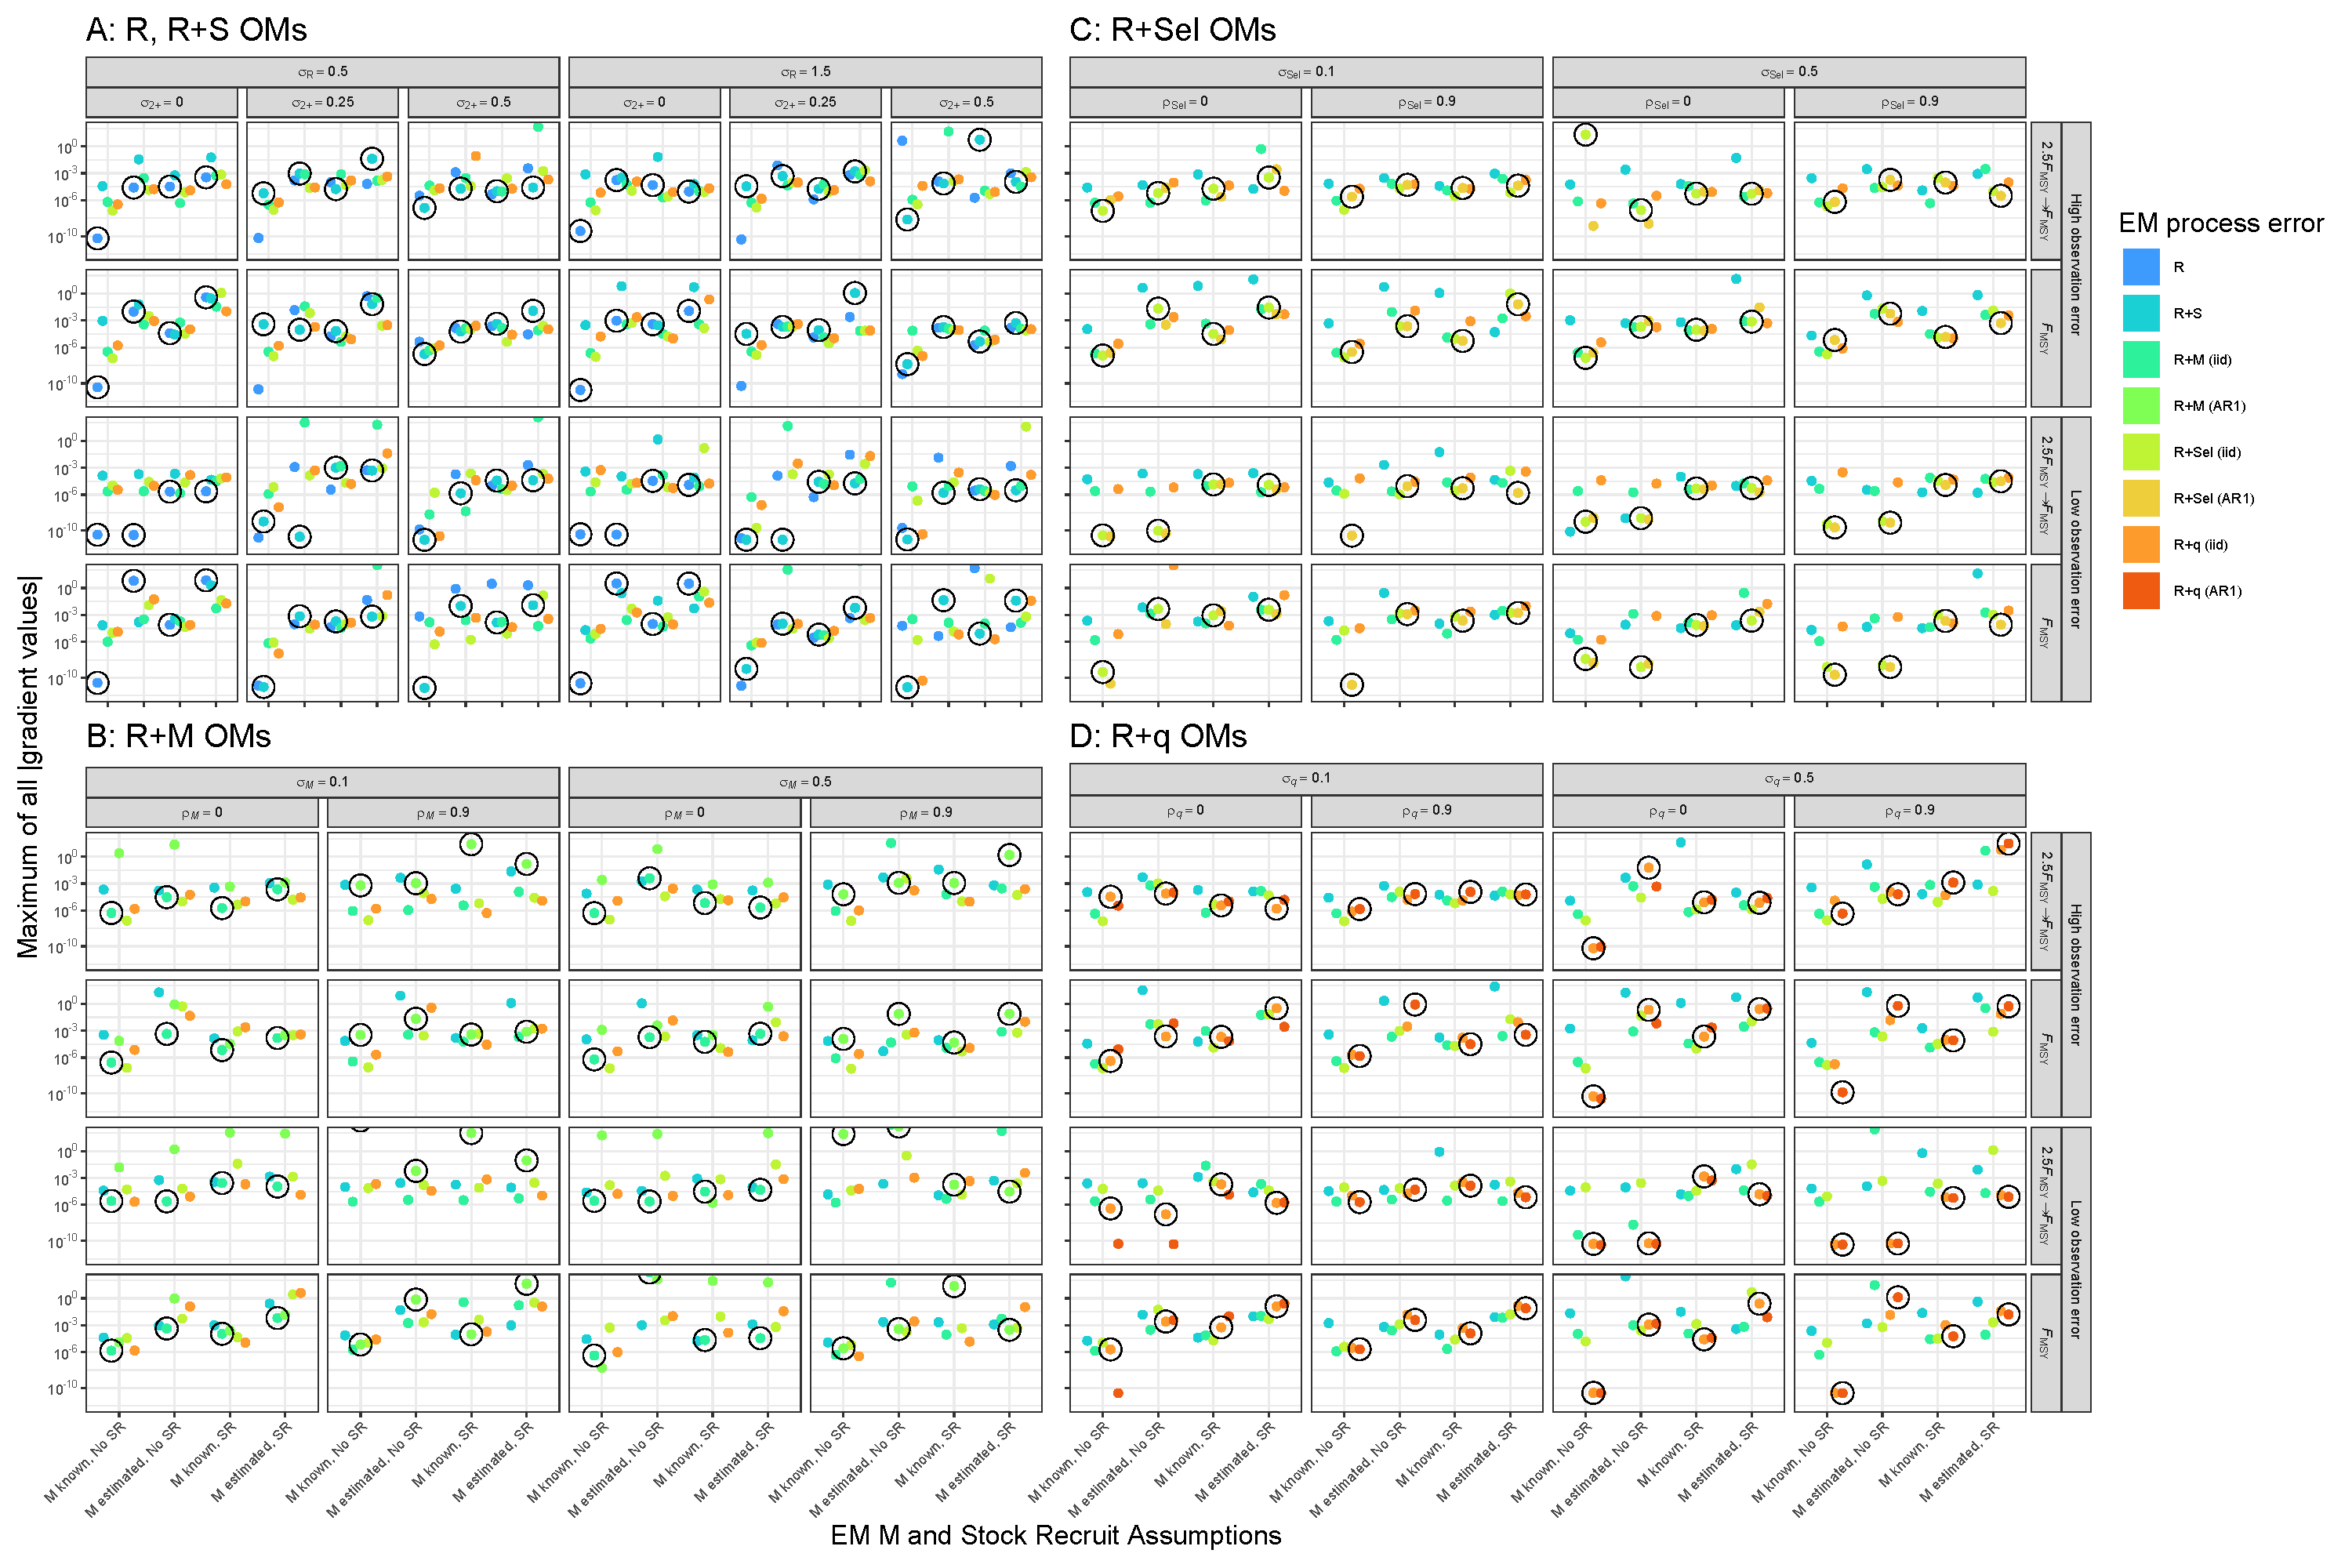
\includegraphics{hess_grad_convergence_plots}
%DIFDELCMD < %%%
\DIFdelendFL \DIFaddbeginFL \begin{tabular}{lrrrrr}
\hline\hline
\multicolumn{1}{l}{\DIFaddFL{Factor}}&\multicolumn{1}{c}{\DIFaddFL{R}}&\multicolumn{1}{c}{\DIFaddFL{R+S}}&\multicolumn{1}{c}{\DIFaddFL{R+M}}&\multicolumn{1}{c}{\DIFaddFL{R+Sel}}&\multicolumn{1}{c}{\DIFaddFL{R+q}}\tabularnewline
\hline
\DIFaddFL{EM Process Error}&\DIFaddFL{30.40}& \DIFaddFL{0.45}&\DIFaddFL{17.57}&\DIFaddFL{16.04}&\DIFaddFL{24.03}\tabularnewline
\DIFaddFL{EM $M$ Assumption}& \DIFaddFL{2.38}&\DIFaddFL{24.11}& \DIFaddFL{4.42}& \DIFaddFL{1.02}& \DIFaddFL{2.66}\tabularnewline
\DIFaddFL{EM SR Assumption}& \DIFaddFL{1.80}& \DIFaddFL{0.32}& \DIFaddFL{0.96}& \DIFaddFL{3.38}& \DIFaddFL{2.13}\tabularnewline
\DIFaddFL{OM Obs. Error}& \DIFaddFL{0.12}& \DIFaddFL{0.77}& \DIFaddFL{0.33}& \DIFaddFL{1.76}& \DIFaddFL{0.28}\tabularnewline
\DIFaddFL{OM $F$ History}& \DIFaddFL{3.51}& \DIFaddFL{6.33}& \DIFaddFL{2.36}& \DIFaddFL{5.86}& \DIFaddFL{5.30}\tabularnewline
\DIFaddFL{OM $\sigma_R$}&\DIFaddFL{\textless  0.01}&\DIFaddFL{\textless  0.01}&\DIFaddFL{--}&\DIFaddFL{--}&\DIFaddFL{--}\tabularnewline
\DIFaddFL{OM $\sigma_{2+}$ }&\DIFaddFL{--}&\DIFaddFL{\textless  0.01}&\DIFaddFL{--}&\DIFaddFL{--}&\DIFaddFL{--}\tabularnewline
\DIFaddFL{OM $\sigma_M$}&\DIFaddFL{--}&\DIFaddFL{--}& \DIFaddFL{0.39}&\DIFaddFL{--}&\DIFaddFL{--}\tabularnewline
\DIFaddFL{OM $\rho_R$}&\DIFaddFL{--}&\DIFaddFL{--}& \DIFaddFL{0.09}&\DIFaddFL{--}&\DIFaddFL{--}\tabularnewline
\DIFaddFL{OM $\sigma_{Sel}$}&\DIFaddFL{--}&\DIFaddFL{--}&\DIFaddFL{--}& \DIFaddFL{1.08}&\DIFaddFL{--}\tabularnewline
\DIFaddFL{OM $\rho_{Sel}$}&\DIFaddFL{--}&\DIFaddFL{--}&\DIFaddFL{--}& \DIFaddFL{0.01}&\DIFaddFL{--}\tabularnewline
\DIFaddFL{OM $\sigma_q$}&\DIFaddFL{--}&\DIFaddFL{--}&\DIFaddFL{--}&\DIFaddFL{--}& \DIFaddFL{0.06}\tabularnewline
\DIFaddFL{OM $\rho_q$}&\DIFaddFL{--}&\DIFaddFL{--}&\DIFaddFL{--}&\DIFaddFL{--}&\DIFaddFL{\textless  0.01}\tabularnewline
\DIFaddFL{All factors}&\DIFaddFL{43.69}&\DIFaddFL{35.72}&\DIFaddFL{29.33}&\DIFaddFL{34.57}&\DIFaddFL{40.69}\tabularnewline
\DIFaddFL{+ All Two Way}&\DIFaddFL{50.53}&\DIFaddFL{42.99}&\DIFaddFL{43.91}&\DIFaddFL{45.93}&\DIFaddFL{48.62}\tabularnewline
\DIFaddFL{+ All Three Way}&\DIFaddFL{52.30}&\DIFaddFL{48.41}&\DIFaddFL{46.81}&\DIFaddFL{47.71}&\DIFaddFL{50.40}\tabularnewline
\hline
\end{tabular}\DIFaddendFL \end{center}
\DIFdelbeginFL %DIFDELCMD < \caption{%
{%DIFAUXCMD
\DIFdelFL{The maximum of the absolute values of all gradient values for all fits that provided hessian-based standard errors across all simuated data sets of a given OM configuration (A: R and R+S, B: R+M, C: R+Sel, or D: R+q).  Results are conditional on EM fits with alternative process error type (colored points and lines), median natural mortality (estimated or known) and recruitment assumptions (Beverton-Holt stock-recruit relationship or not). Circled values indicate results where the EM process error structure matches that of the operating model and vertical lines represent 95\% confidence intervals.}}%DIFAUXCMD
%DIFDELCMD < \label{hess_grad}
%DIFDELCMD < \end{figure}
%DIFDELCMD < \end{landscape}
%DIFDELCMD < %%%
\DIFdelend \DIFaddbegin }
\end{table}
\DIFaddend 

\DIFdelbegin %DIFDELCMD < \begin{landscape}
%DIFDELCMD < \begin{figure}
%DIFDELCMD < %%%
\DIFdelendFL \DIFaddbeginFL \begin{table}
\caption{\DIFaddFL{For each OM process error type (columns), percent reduction in deviance for linear regression models fit to transformed Mohn's $\rho$ values for each simulation (Eq. \ref{bias_regression_response}) for fishing mortality averaged over all age classes with each OM and EM factor (rows) included individually, combined, and with second and third order interactions.}}\label{mohns_rho_F_PRD_table}
{\DIFaddendFL \begin{center}
\DIFdelbeginFL %DIFDELCMD < 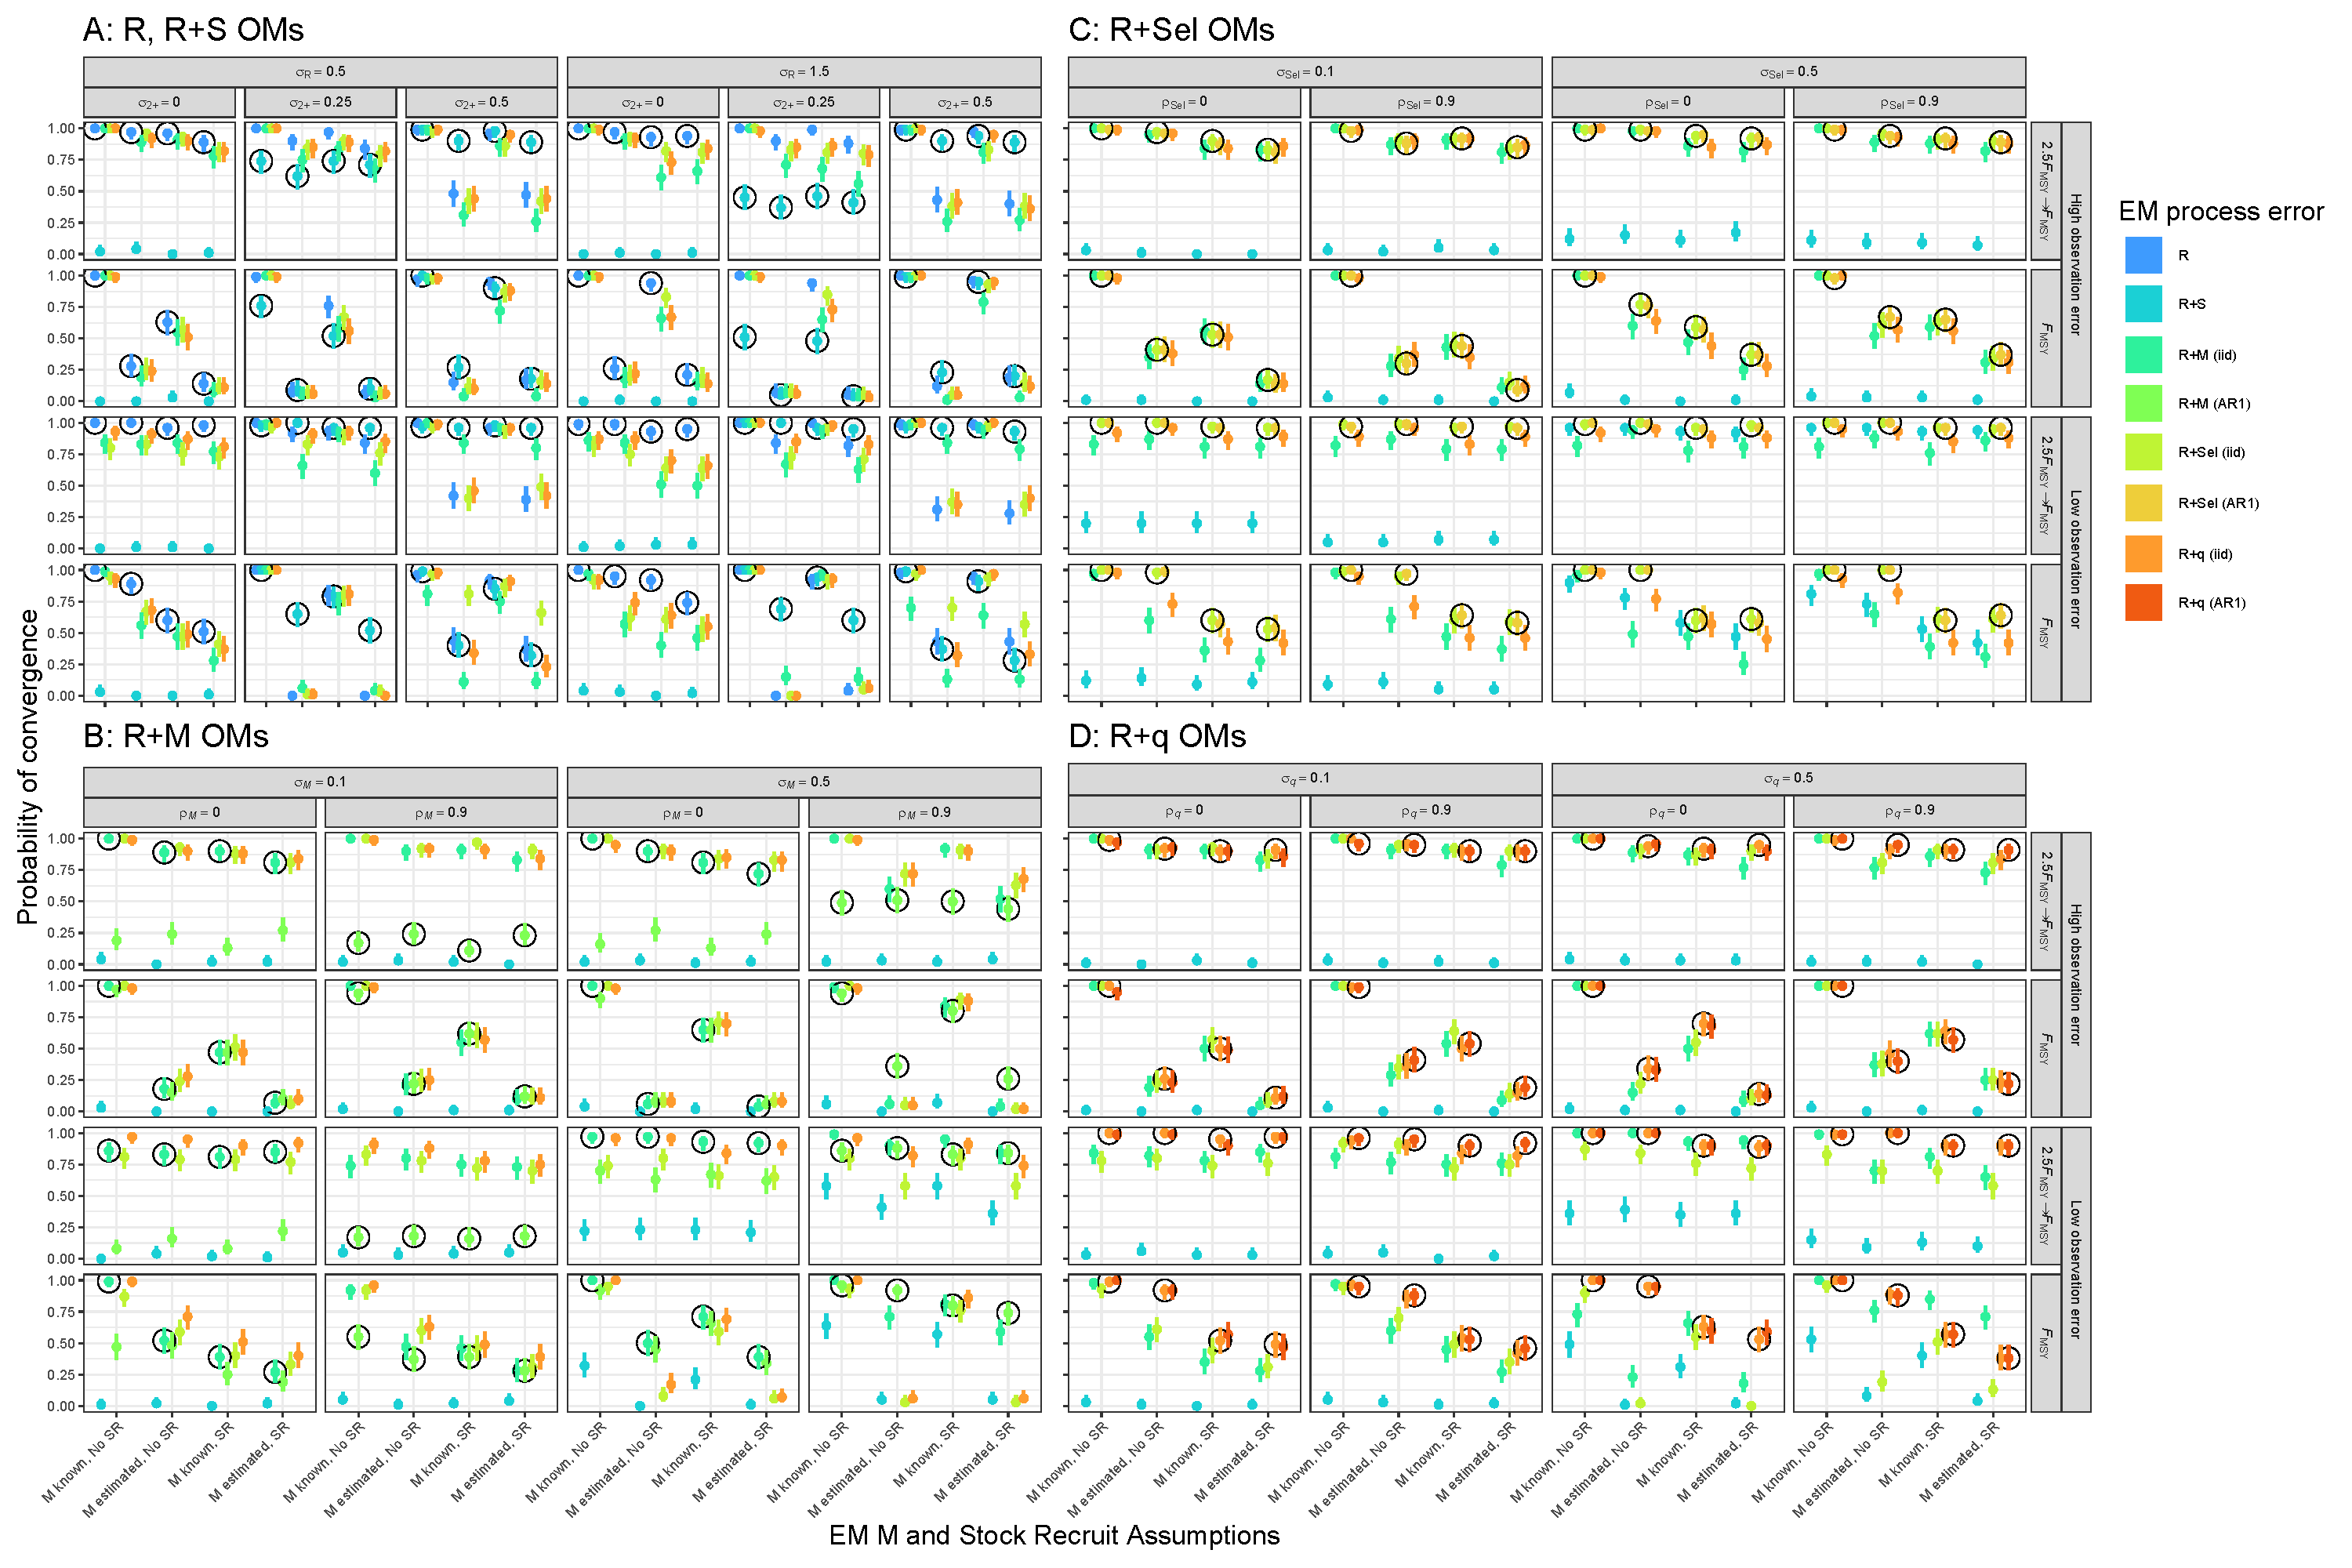
\includegraphics{type_3_convergence_plots}
%DIFDELCMD < %%%
\DIFdelendFL \DIFaddbeginFL \begin{tabular}{lrrrrr}
\hline\hline
\multicolumn{1}{l}{\DIFaddFL{Factor}}&\multicolumn{1}{c}{\DIFaddFL{R}}&\multicolumn{1}{c}{\DIFaddFL{R+S}}&\multicolumn{1}{c}{\DIFaddFL{R+M}}&\multicolumn{1}{c}{\DIFaddFL{R+Sel}}&\multicolumn{1}{c}{\DIFaddFL{R+q}}\tabularnewline
\hline
\DIFaddFL{EM $M$ Assumption}&\DIFaddFL{0.06}&\DIFaddFL{0.09}&\DIFaddFL{0.01}&\DIFaddFL{0.12}&\DIFaddFL{0.01}\tabularnewline
\DIFaddFL{EM SR assumption}&\DIFaddFL{0.01}&\DIFaddFL{\textless  0.01}&\DIFaddFL{0.01}&\DIFaddFL{0.02}&\DIFaddFL{0.01}\tabularnewline
\DIFaddFL{EM Process Error}&\DIFaddFL{0.03}&\DIFaddFL{0.07}&\DIFaddFL{0.02}&\DIFaddFL{0.06}&\DIFaddFL{0.03}\tabularnewline
\DIFaddFL{OM Obs. Error}&\DIFaddFL{0.16}&\DIFaddFL{0.10}&\DIFaddFL{0.05}&\DIFaddFL{0.02}&\DIFaddFL{0.07}\tabularnewline
\DIFaddFL{OM $F$ History}&\DIFaddFL{0.07}&\DIFaddFL{0.02}&\DIFaddFL{0.03}&\DIFaddFL{0.24}&\DIFaddFL{0.03}\tabularnewline
\DIFaddFL{OM $\sigma_R$}&\DIFaddFL{\textless  0.01}&\DIFaddFL{0.01}&\DIFaddFL{--}&\DIFaddFL{--}&\DIFaddFL{--}\tabularnewline
\DIFaddFL{OM $\sigma_{2+}$ }&\DIFaddFL{--}&\DIFaddFL{0.09}&\DIFaddFL{--}&\DIFaddFL{--}&\DIFaddFL{--}\tabularnewline
\DIFaddFL{OM $\sigma_M$}&\DIFaddFL{--}&\DIFaddFL{--}&\DIFaddFL{\textless  0.01}&\DIFaddFL{--}&\DIFaddFL{--}\tabularnewline
\DIFaddFL{OM $\rho_R$}&\DIFaddFL{--}&\DIFaddFL{--}&\DIFaddFL{\textless  0.01}&\DIFaddFL{--}&\DIFaddFL{--}\tabularnewline
\DIFaddFL{OM $\sigma_{Sel}$}&\DIFaddFL{--}&\DIFaddFL{--}&\DIFaddFL{--}&\DIFaddFL{0.01}&\DIFaddFL{--}\tabularnewline
\DIFaddFL{OM $\rho_{Sel}$}&\DIFaddFL{--}&\DIFaddFL{--}&\DIFaddFL{--}&\DIFaddFL{\textless  0.01}&\DIFaddFL{--}\tabularnewline
\DIFaddFL{OM $\sigma_q$}&\DIFaddFL{--}&\DIFaddFL{--}&\DIFaddFL{--}&\DIFaddFL{--}&\DIFaddFL{\textless  0.01}\tabularnewline
\DIFaddFL{OM $\rho_q$}&\DIFaddFL{--}&\DIFaddFL{--}&\DIFaddFL{--}&\DIFaddFL{--}&\DIFaddFL{0.01}\tabularnewline
\DIFaddFL{All factors}&\DIFaddFL{0.32}&\DIFaddFL{0.38}&\DIFaddFL{0.12}&\DIFaddFL{0.48}&\DIFaddFL{0.15}\tabularnewline
\DIFaddFL{+ All Two Way}&\DIFaddFL{0.65}&\DIFaddFL{0.67}&\DIFaddFL{0.30}&\DIFaddFL{0.95}&\DIFaddFL{0.43}\tabularnewline
\DIFaddFL{+ All Three Way}&\DIFaddFL{1.18}&\DIFaddFL{1.11}&\DIFaddFL{0.63}&\DIFaddFL{1.34}&\DIFaddFL{0.90}\tabularnewline
\hline
\end{tabular}\DIFaddendFL \end{center}
\DIFdelbeginFL %DIFDELCMD < \caption{%
{%DIFAUXCMD
\DIFdelFL{Probability of estimating models providing maximum absolute values of gradients less than $10^{-6}$ assuming alternative process error (colored points and lines), and median natural mortality (estimated or known) and Beverton-Holt stock-recruit relationships (estimated or not; along x-axis) when fitted to operating models that have R and R+S (A), R+Sel (B), R+M (C), or R+q (D) process error structures. Circled values indicate results where the EM process error structure matches that of the operating model and vertical lines represent 95\% confidence intervals.}}%DIFAUXCMD
%DIFDELCMD < \label{gradient_convergence}
%DIFDELCMD < \end{figure}
%DIFDELCMD < \end{landscape}
%DIFDELCMD < %%%
\DIFdelend \DIFaddbegin }
\end{table}
\DIFaddend 

\DIFdelbegin %DIFDELCMD < \begin{landscape}
%DIFDELCMD < \begin{figure}
%DIFDELCMD < %%%
\DIFdelendFL \DIFaddbeginFL \begin{table}
\caption{\DIFaddFL{For each OM process error type (columns), percent reduction in deviance for linear regression models fit to transformed Mohn's $\rho$ values for each simulation (Eq. \ref{bias_regression_response}) for recruitment with each OM and EM factor (rows) included individually, combined, and with second and third order interactions.}}\label{mohns_rho_R_PRD_table}
{\DIFaddendFL \begin{center}
\DIFdelbeginFL %DIFDELCMD < 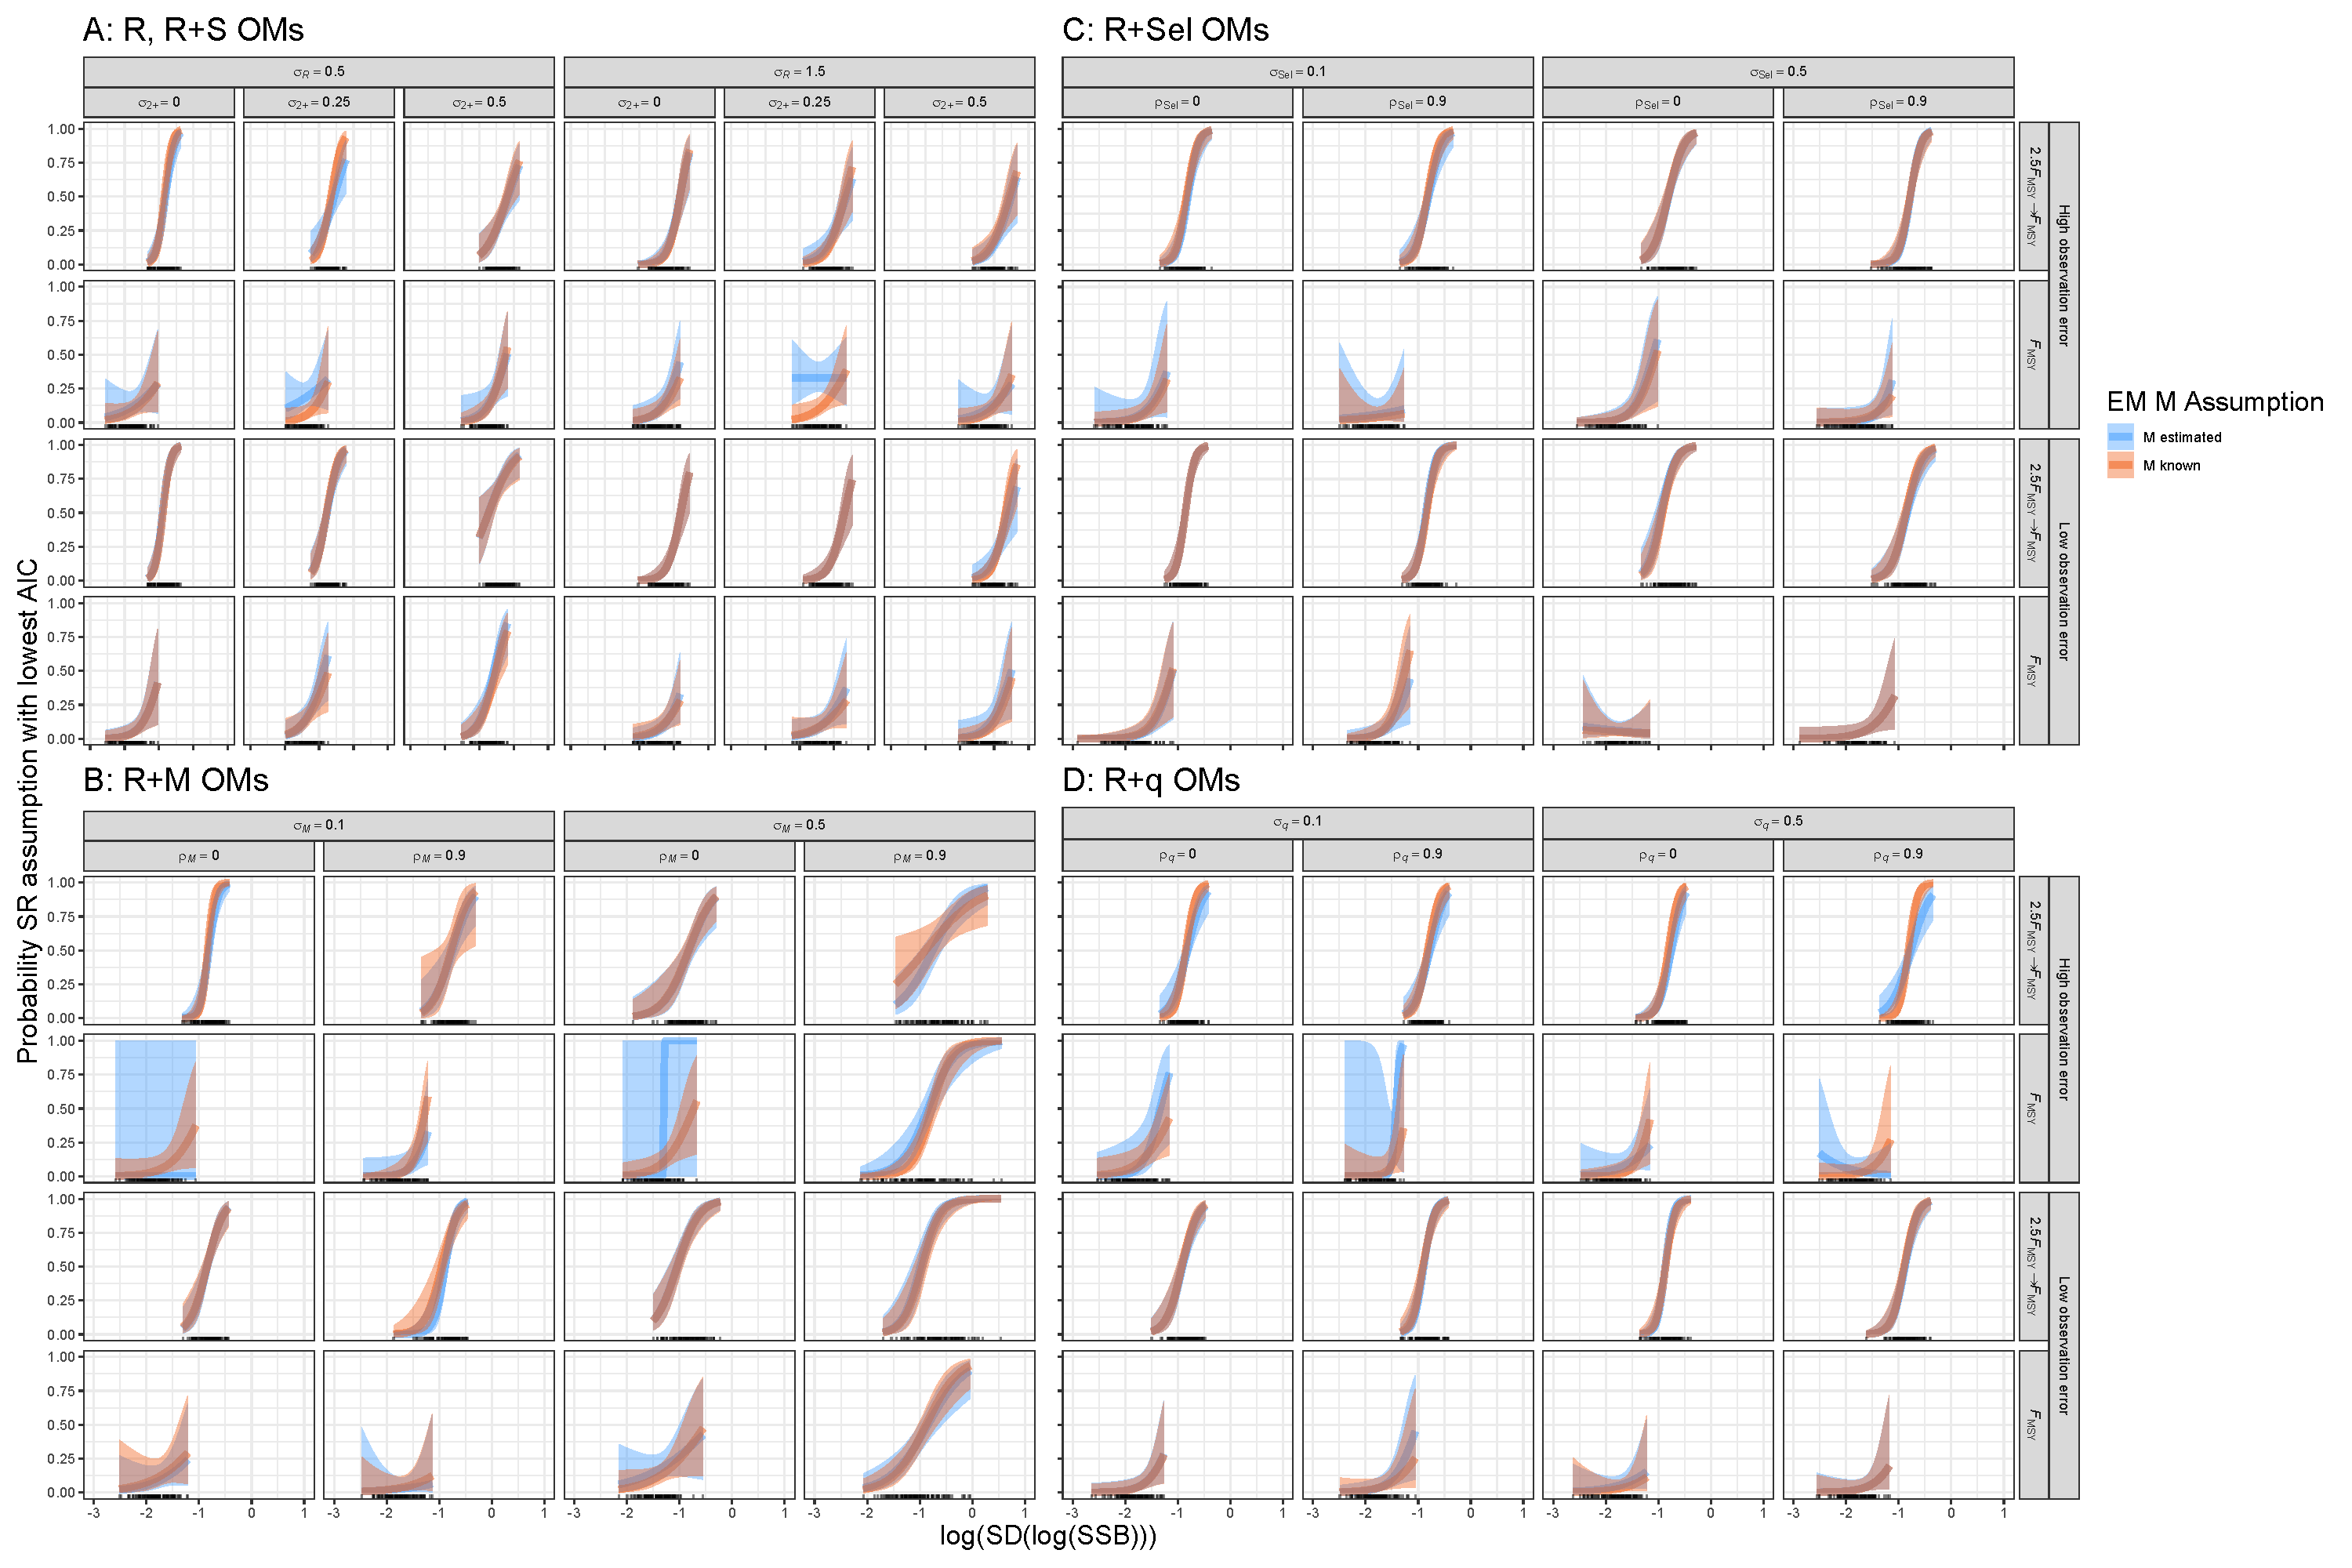
\includegraphics{sr_aic_plots}
%DIFDELCMD < %%%
\DIFdelendFL \DIFaddbeginFL \begin{tabular}{lrrrrr}
\hline\hline
\multicolumn{1}{l}{\DIFaddFL{Factor}}&\multicolumn{1}{c}{\DIFaddFL{R}}&\multicolumn{1}{c}{\DIFaddFL{R+S}}&\multicolumn{1}{c}{\DIFaddFL{R+M}}&\multicolumn{1}{c}{\DIFaddFL{R+Sel}}&\multicolumn{1}{c}{\DIFaddFL{R+q}}\tabularnewline
\hline
\DIFaddFL{EM $M$ Assumption}&\DIFaddFL{0.86}&\DIFaddFL{0.56}&\DIFaddFL{0.16}&\DIFaddFL{1.00}&\DIFaddFL{1.27}\tabularnewline
\DIFaddFL{EM SR assumption}&\DIFaddFL{\textless  0.01}&\DIFaddFL{0.02}&\DIFaddFL{0.01}&\DIFaddFL{0.01}&\DIFaddFL{0.01}\tabularnewline
\DIFaddFL{EM Process Error}&\DIFaddFL{0.01}&\DIFaddFL{0.59}&\DIFaddFL{0.18}&\DIFaddFL{0.07}&\DIFaddFL{0.04}\tabularnewline
\DIFaddFL{OM Obs. Error}&\DIFaddFL{0.34}&\DIFaddFL{0.01}&\DIFaddFL{0.08}&\DIFaddFL{0.24}&\DIFaddFL{0.27}\tabularnewline
\DIFaddFL{OM $F$ History}&\DIFaddFL{0.91}&\DIFaddFL{0.22}&\DIFaddFL{0.06}&\DIFaddFL{1.20}&\DIFaddFL{1.67}\tabularnewline
\DIFaddFL{OM $\sigma_R$}&\DIFaddFL{\textless  0.01}&\DIFaddFL{0.14}&\DIFaddFL{--}&\DIFaddFL{--}&\DIFaddFL{--}\tabularnewline
\DIFaddFL{OM $\sigma_{2+}$ }&\DIFaddFL{--}&\DIFaddFL{0.11}&\DIFaddFL{--}&\DIFaddFL{--}&\DIFaddFL{--}\tabularnewline
\DIFaddFL{OM $\sigma_M$}&\DIFaddFL{--}&\DIFaddFL{--}&\DIFaddFL{0.01}&\DIFaddFL{--}&\DIFaddFL{--}\tabularnewline
\DIFaddFL{OM $\rho_R$}&\DIFaddFL{--}&\DIFaddFL{--}&\DIFaddFL{\textless  0.01}&\DIFaddFL{--}&\DIFaddFL{--}\tabularnewline
\DIFaddFL{OM $\sigma_{Sel}$}&\DIFaddFL{--}&\DIFaddFL{--}&\DIFaddFL{--}&\DIFaddFL{0.01}&\DIFaddFL{--}\tabularnewline
\DIFaddFL{OM $\rho_{Sel}$}&\DIFaddFL{--}&\DIFaddFL{--}&\DIFaddFL{--}&\DIFaddFL{0.01}&\DIFaddFL{--}\tabularnewline
\DIFaddFL{OM $\sigma_q$}&\DIFaddFL{--}&\DIFaddFL{--}&\DIFaddFL{--}&\DIFaddFL{--}&\DIFaddFL{0.01}\tabularnewline
\DIFaddFL{OM $\rho_q$}&\DIFaddFL{--}&\DIFaddFL{--}&\DIFaddFL{--}&\DIFaddFL{--}&\DIFaddFL{0.01}\tabularnewline
\DIFaddFL{All factors}&\DIFaddFL{2.28}&\DIFaddFL{1.74}&\DIFaddFL{0.51}&\DIFaddFL{2.66}&\DIFaddFL{3.51}\tabularnewline
\DIFaddFL{+ All Two Way}&\DIFaddFL{4.20}&\DIFaddFL{2.74}&\DIFaddFL{1.08}&\DIFaddFL{5.08}&\DIFaddFL{6.51}\tabularnewline
\DIFaddFL{+ All Three Way}&\DIFaddFL{4.83}&\DIFaddFL{3.79}&\DIFaddFL{1.79}&\DIFaddFL{6.03}&\DIFaddFL{7.82}\tabularnewline
\hline
\end{tabular}\DIFaddendFL \end{center}
\DIFdelbeginFL %DIFDELCMD < \caption{%
{%DIFAUXCMD
\DIFdelFL{Estimated probability of lowest AIC from logistic regression on the log-standard deviation of the true log(SSB) in each simulation for estimating model with Beverton-Holt stock-recruit relationships, rather than the otherwise equivalent EM without the stock-recruit relationship. Results are conditional on alternative assumptions for median natural mortality (estimated or known) and on EMs having the correct process error structure: R and R+S (A), R+Sel (B), R+M (C), or R+q (D). Rug along x-axis denotes $SD(\log(SSB))$ values for each simulation and polygons represent 95\% confidence intervals.}}%DIFAUXCMD
%DIFDELCMD < \label{sr_aic_supp}
%DIFDELCMD < \end{figure}
%DIFDELCMD < \end{landscape}
%DIFDELCMD < %%%
\DIFdelend \DIFaddbegin }
\end{table}
\DIFaddend 

\DIFdelbegin %DIFDELCMD < \clearpage
%DIFDELCMD < %%%
\DIFdelend \DIFaddbegin \subsubsection*{\DIFadd{Convergence full
results}}\label{convergence-full-results}
\addcontentsline{toc}{subsubsection}{\DIFadd{Convergence full results}}
\DIFaddend 

\DIFdelbegin %DIFDELCMD < \begin{landscape}
%DIFDELCMD < \begin{figure}
%DIFDELCMD < \begin{center}
%DIFDELCMD < 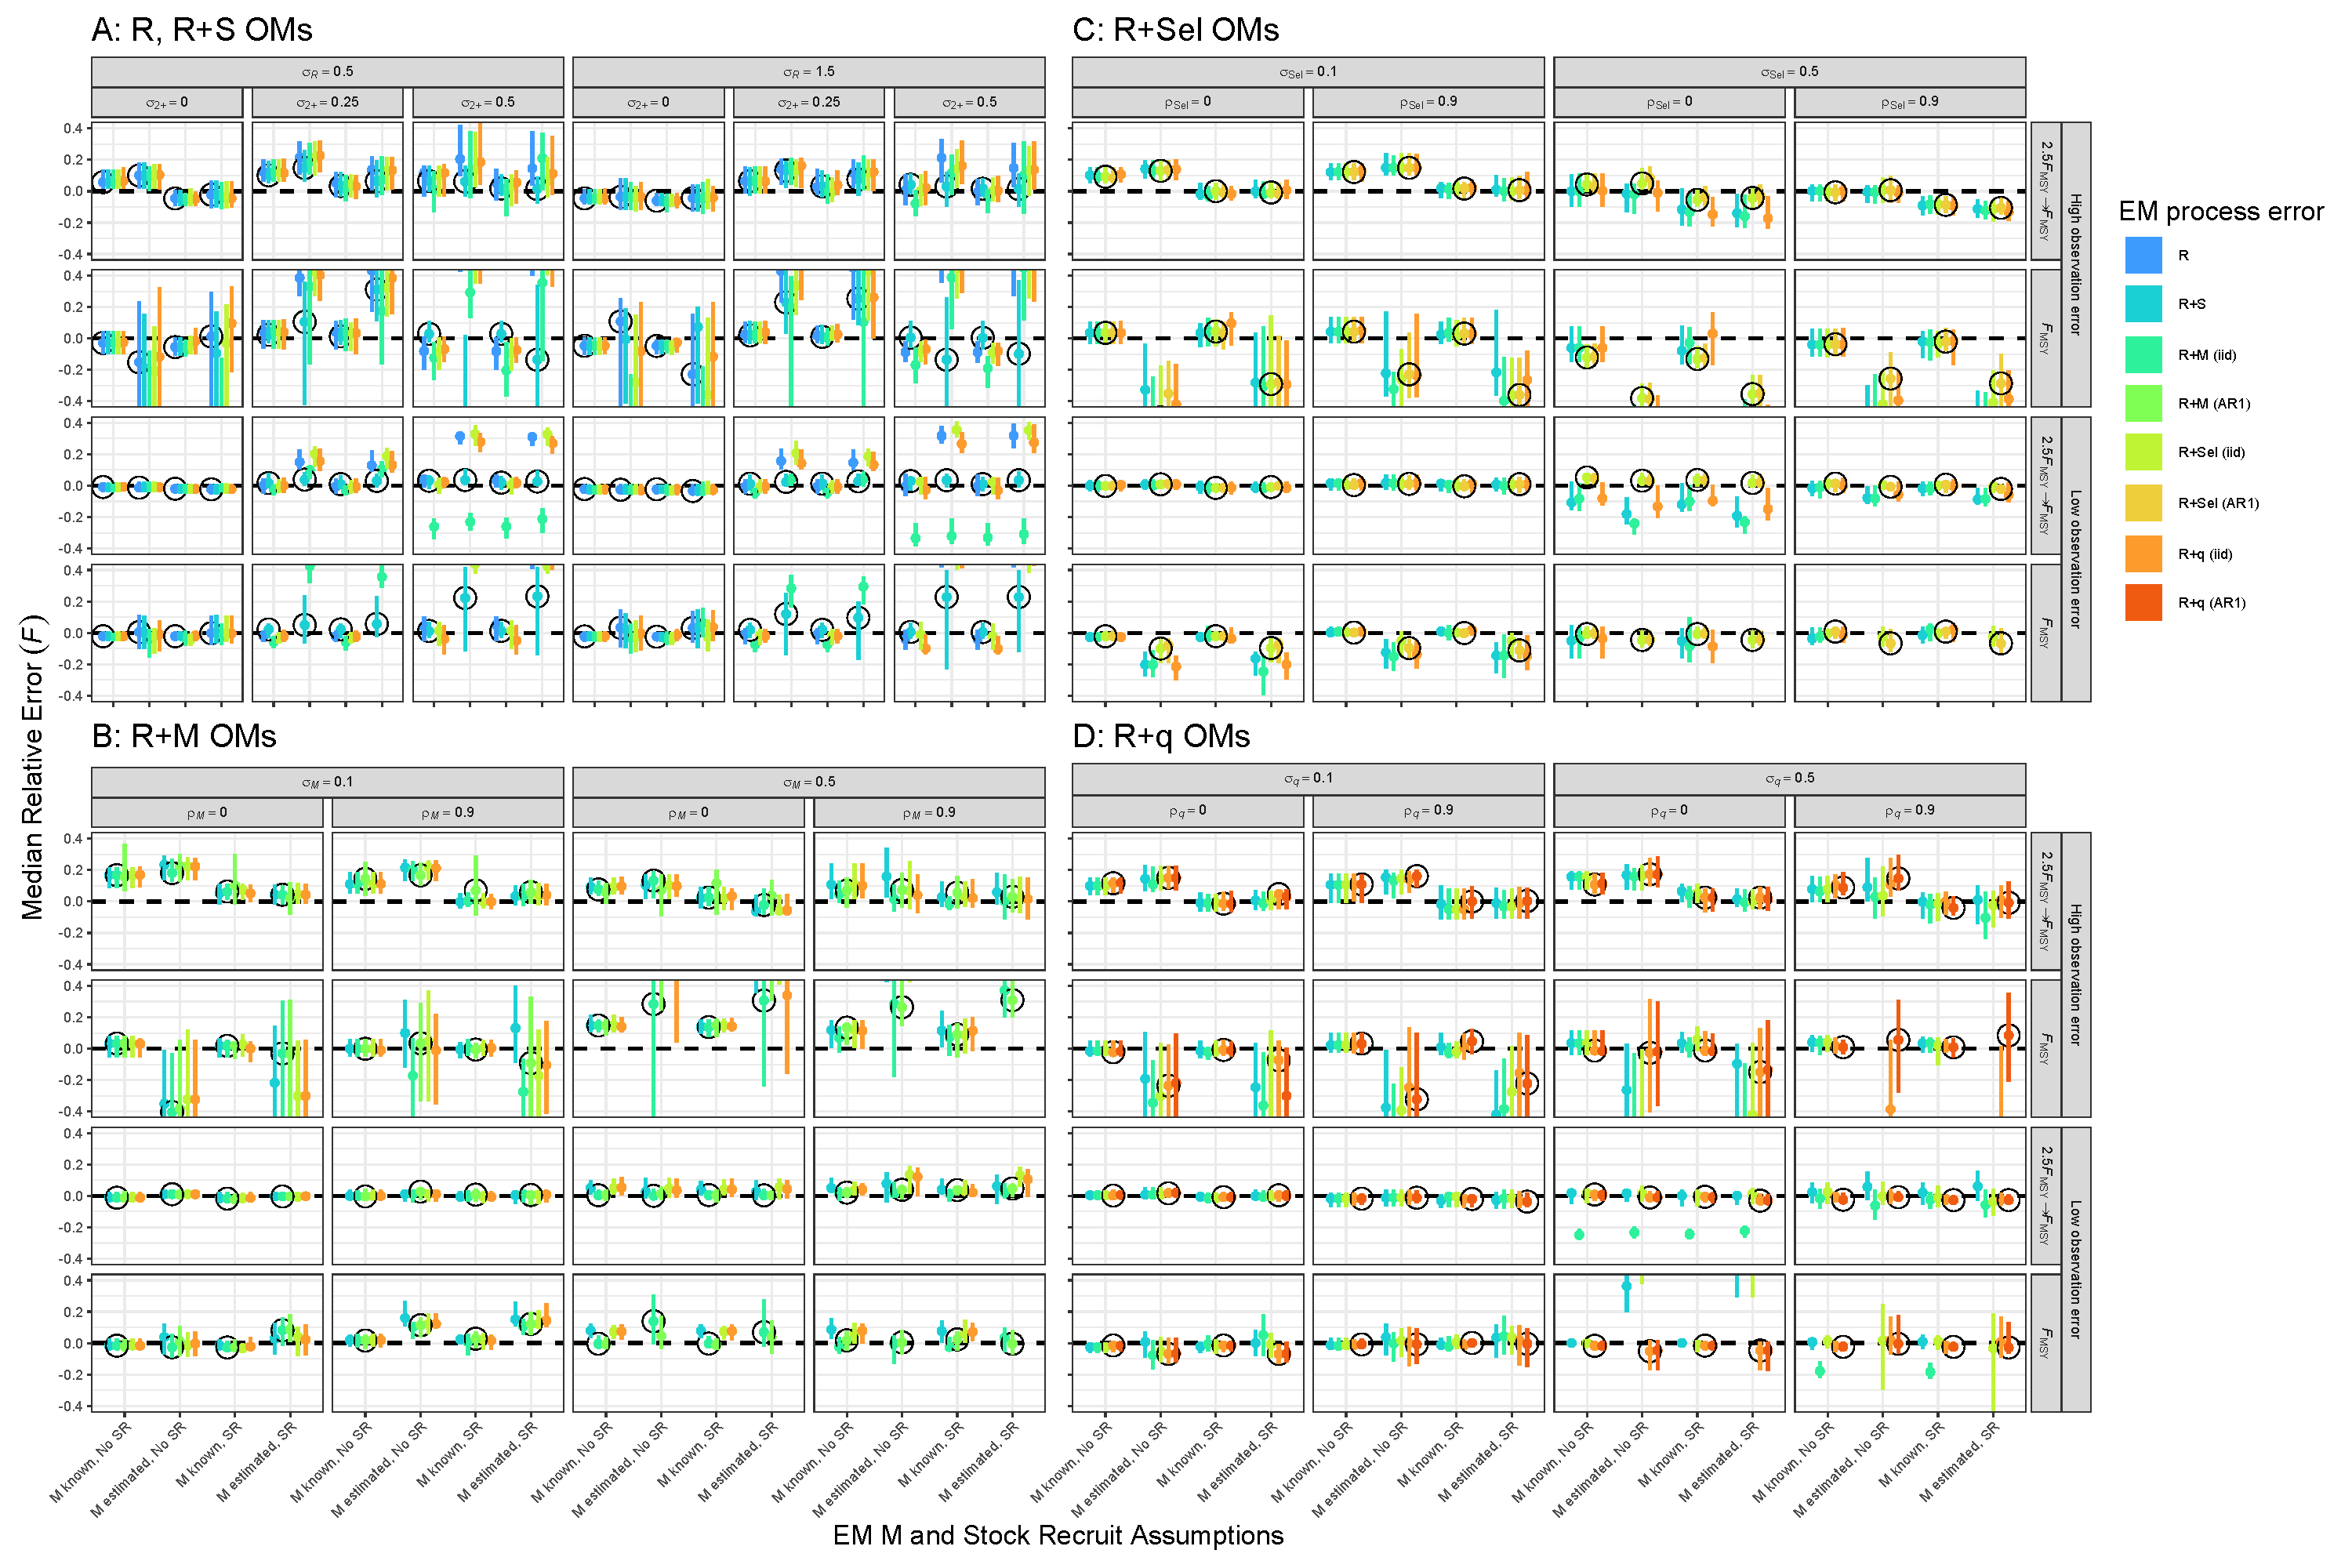
\includegraphics{term_F_bias_plots}
%DIFDELCMD < \end{center}
%DIFDELCMD < %%%
%DIFDELCMD < \caption{%
{%DIFAUXCMD
\DIFdelFL{Median relative error of terminal year fully-selected fishing mortality for estimating models fitted to data sets simulated with alternative process error structures: R and R+S (A), R+Sel (B), R+M (C), or R+q (D). Circled values indicate results where the EM process error structure matches that of the operating model and vertical lines represent 95\% confidence intervals.}}%DIFAUXCMD
%DIFDELCMD < \label{F_rel_error}
%DIFDELCMD < \end{figure}
%DIFDELCMD < \end{landscape}
%DIFDELCMD < %%%
\DIFdelend \DIFaddbegin \DIFadd{For many R and R+S OMs, convergence rate declined when either the median
natural mortality rate or the Beverton-Holt SRR was estimated even when
the process error assumptions of the EMs and OMs matched (Figure
\ref{hessian_SE_convergence}, A). When there was high observation error
and constant fishing pressure (\(F = F_{\text{MSY}}\) for all 40 years),
convergence was poor for of all EM process error configurations other
than R EMs when fitted to R OMs (\(\sigma_{2+} = 0\)) regardless of
whether median natural mortality and SRRs were estimated. Convergence of
R EMs was high for all R and R+S OMs except when there was high
observation error and constant fishing pressure, and when median natural
mortality and SRRs were estimated. R+S EMs fit to R OMs exhibited poor
convergence regardless of whether natural mortality or a SRR was
estimated. R+S EMs fit to R+S OMs had highest convergence rates when
there was contrast in fishing pressure and low observation error.
Convergence rates were high for all EMs when fit to data from R+S OMs
with lower observation error except those where median natural mortality
and/or SRRs were estimated.
}\DIFaddend 

\DIFaddbegin \DIFadd{Convergence of all EMs fitted to R+M OMs was highest when the OMs had
higher natural mortality process error variability, low observation
error, and contrast in fishing pressure (Figure
\ref{hessian_SE_convergence}, B). R+M EMs that estimated autocorrelation
of process errors had poor convergence for R+M OMs when there was low
natural mortality process error variability regardless of
autocorrelation of the simulated process errors. R+S EMs fitted to data
generated from R+M OMs always converged poorly whether or not median
natural mortality and the Beverton-Holt SRR were estimated.
}

\DIFadd{The R+S EMs, in particular, had poor convergence when fit to data
generated from R+Sel OMs with lower selectivity process error
variability or higher observation error (Figure
\ref{hessian_SE_convergence}, C). R+Sel EMs generally converged better
than other EMs for R+Sel OMs with higher process error variability,
lower observation error, and contrast in fishing pressure regardless of
whether median natural mortality or a SRR was estimated.
}

\DIFadd{For R+q OMs, convergence of R+q EMs was generally better than that of
other EMs when there was contrast in fishing pressure (Figure
(\ref{hessian_SE_convergence}, D). Convergence of R+S EMs was generally
worse than that of all other EMs across all OMs whether or not median
natural mortality or a SRR was estimated. Again, convergence probability
generally declined for all EMs when median natural mortality or a SRR
was estimated.
}

\DIFadd{We found a wide range of maximum absolute values of gradients for models
that converged (Figure \ref{hess_grad}). The largest value observed for
a given EM and OM combination was typically \(<10^{-3}\), but many
converged models had values greater than 1. For many OMs, EMs that
assumed the correct process error type and did not estimate median
natural mortality or the Beverton-Holt SRR produced the lowest gradient
values.
}

\DIFaddend \begin{landscape}
\begin{figure}
\begin{center}
\DIFdelbeginFL %DIFDELCMD < 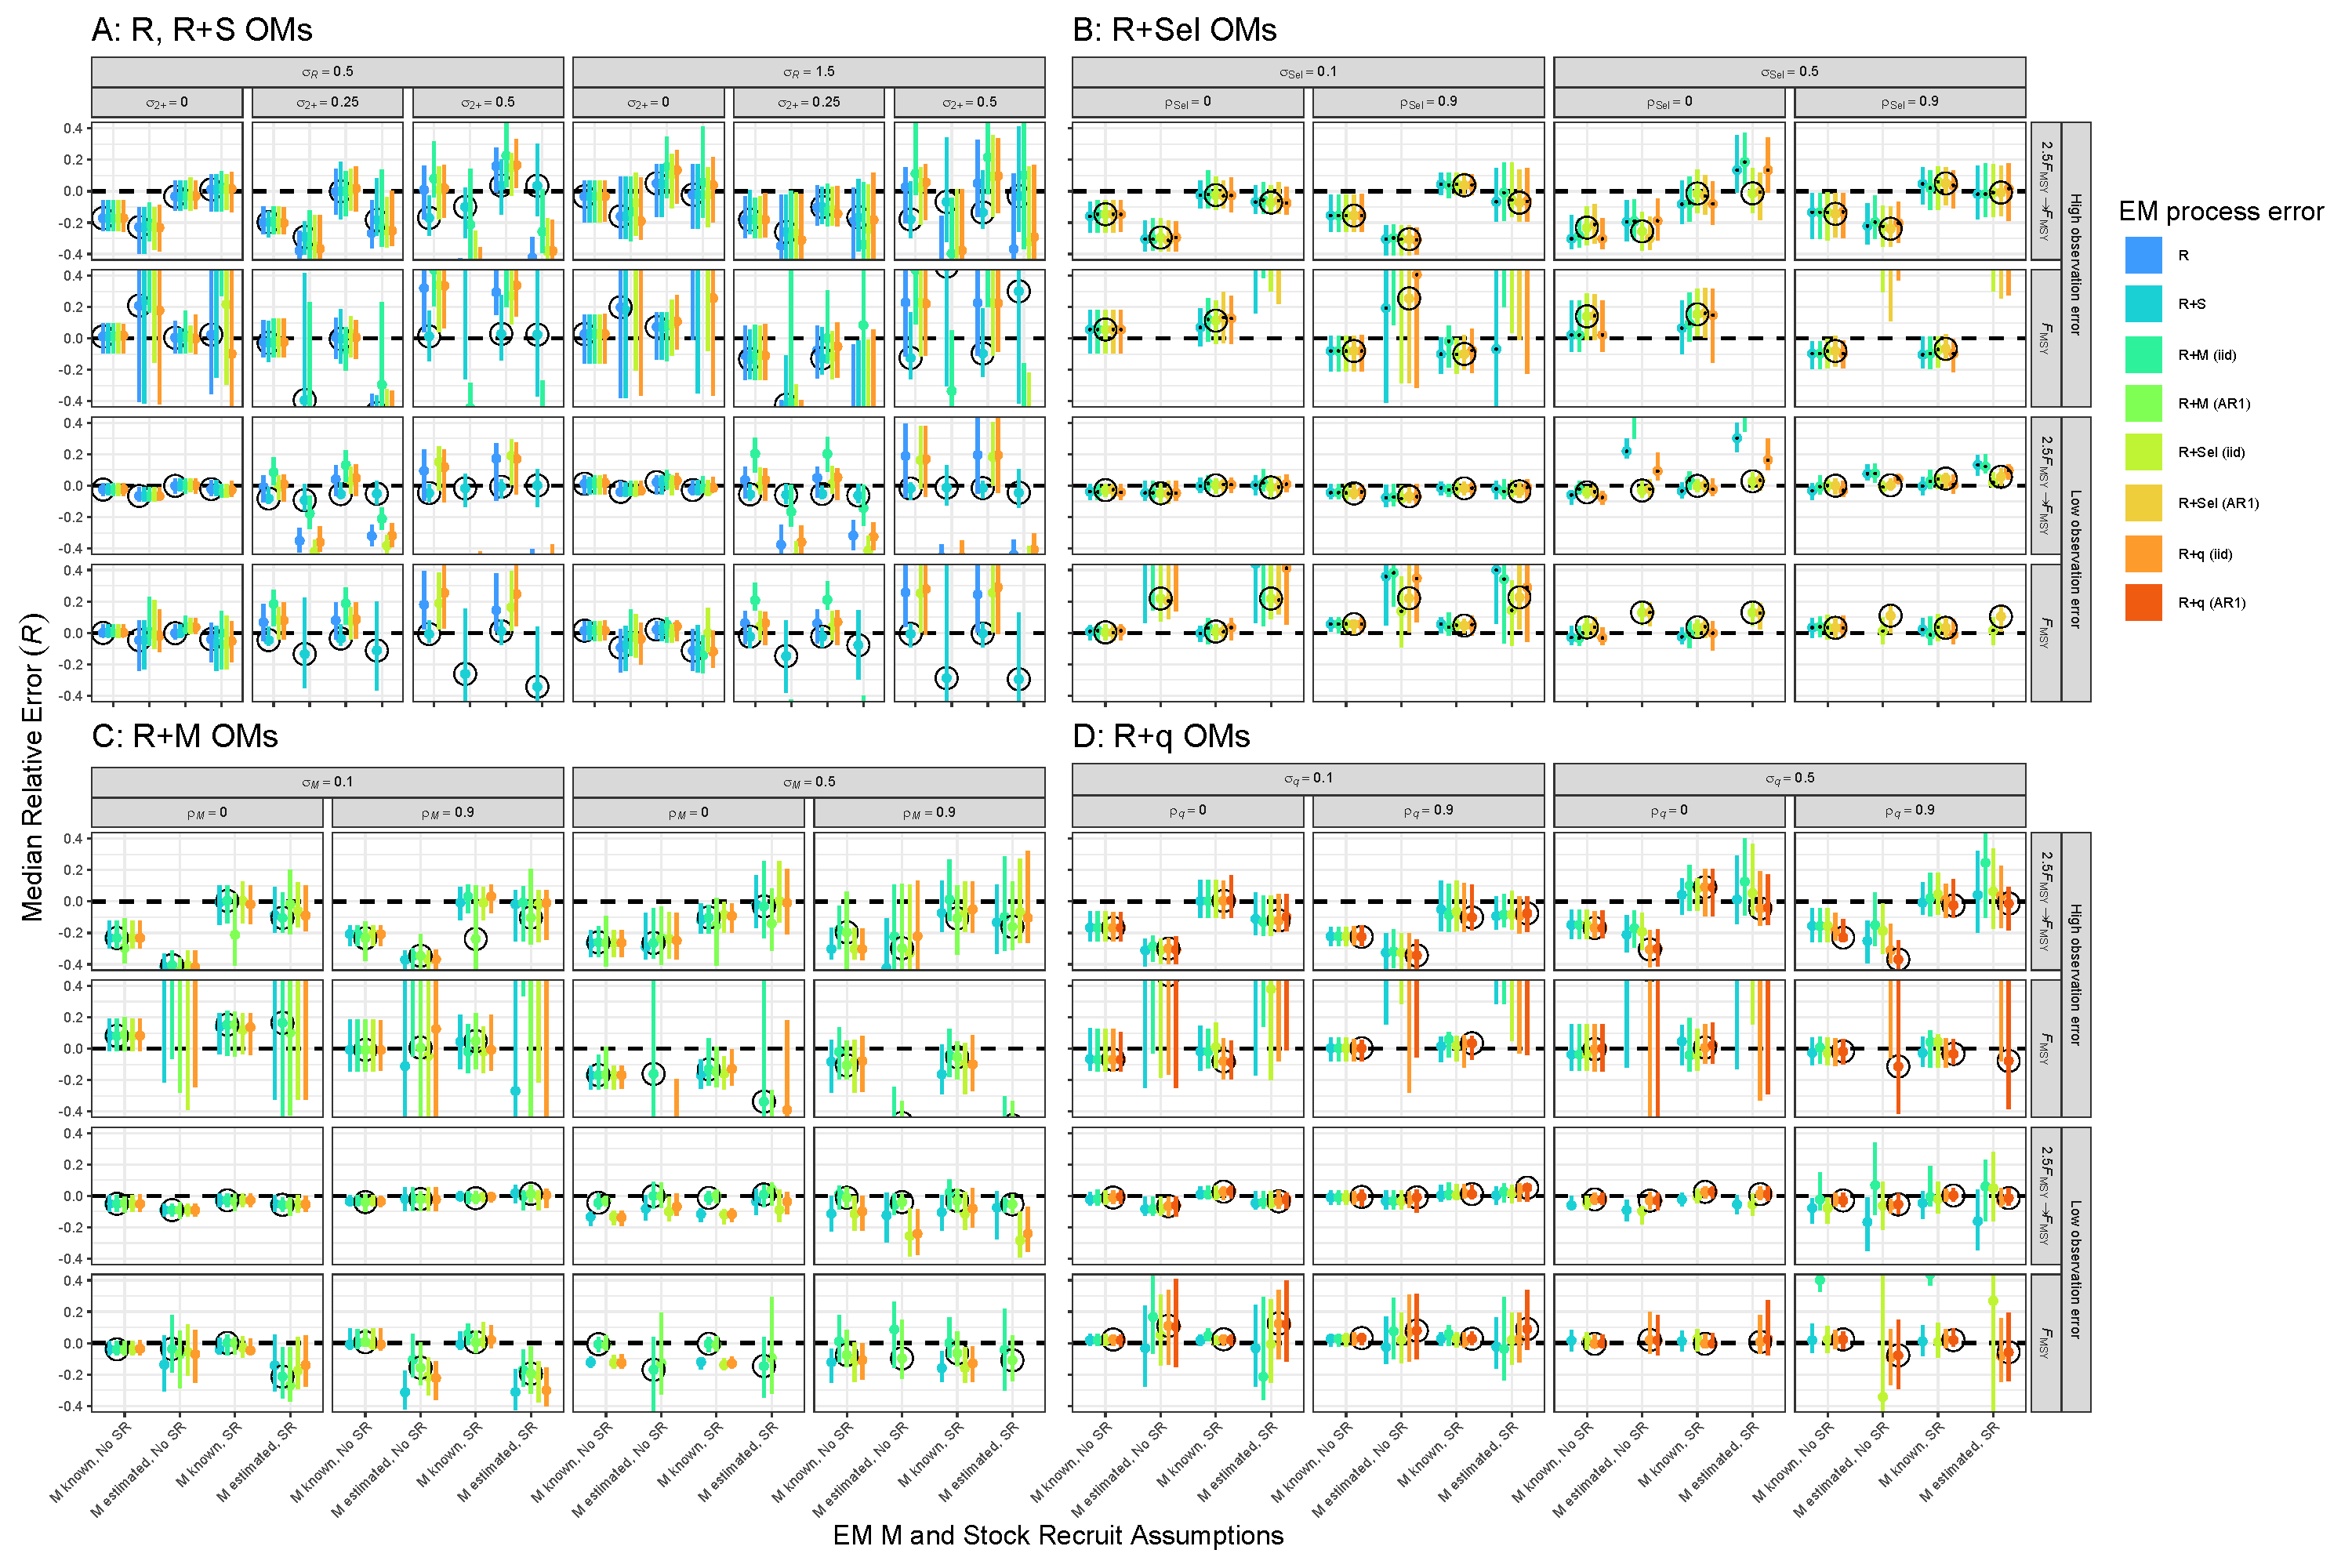
\includegraphics{term_R_bias_plots}
%DIFDELCMD < %%%
\DIFdelendFL \DIFaddbeginFL 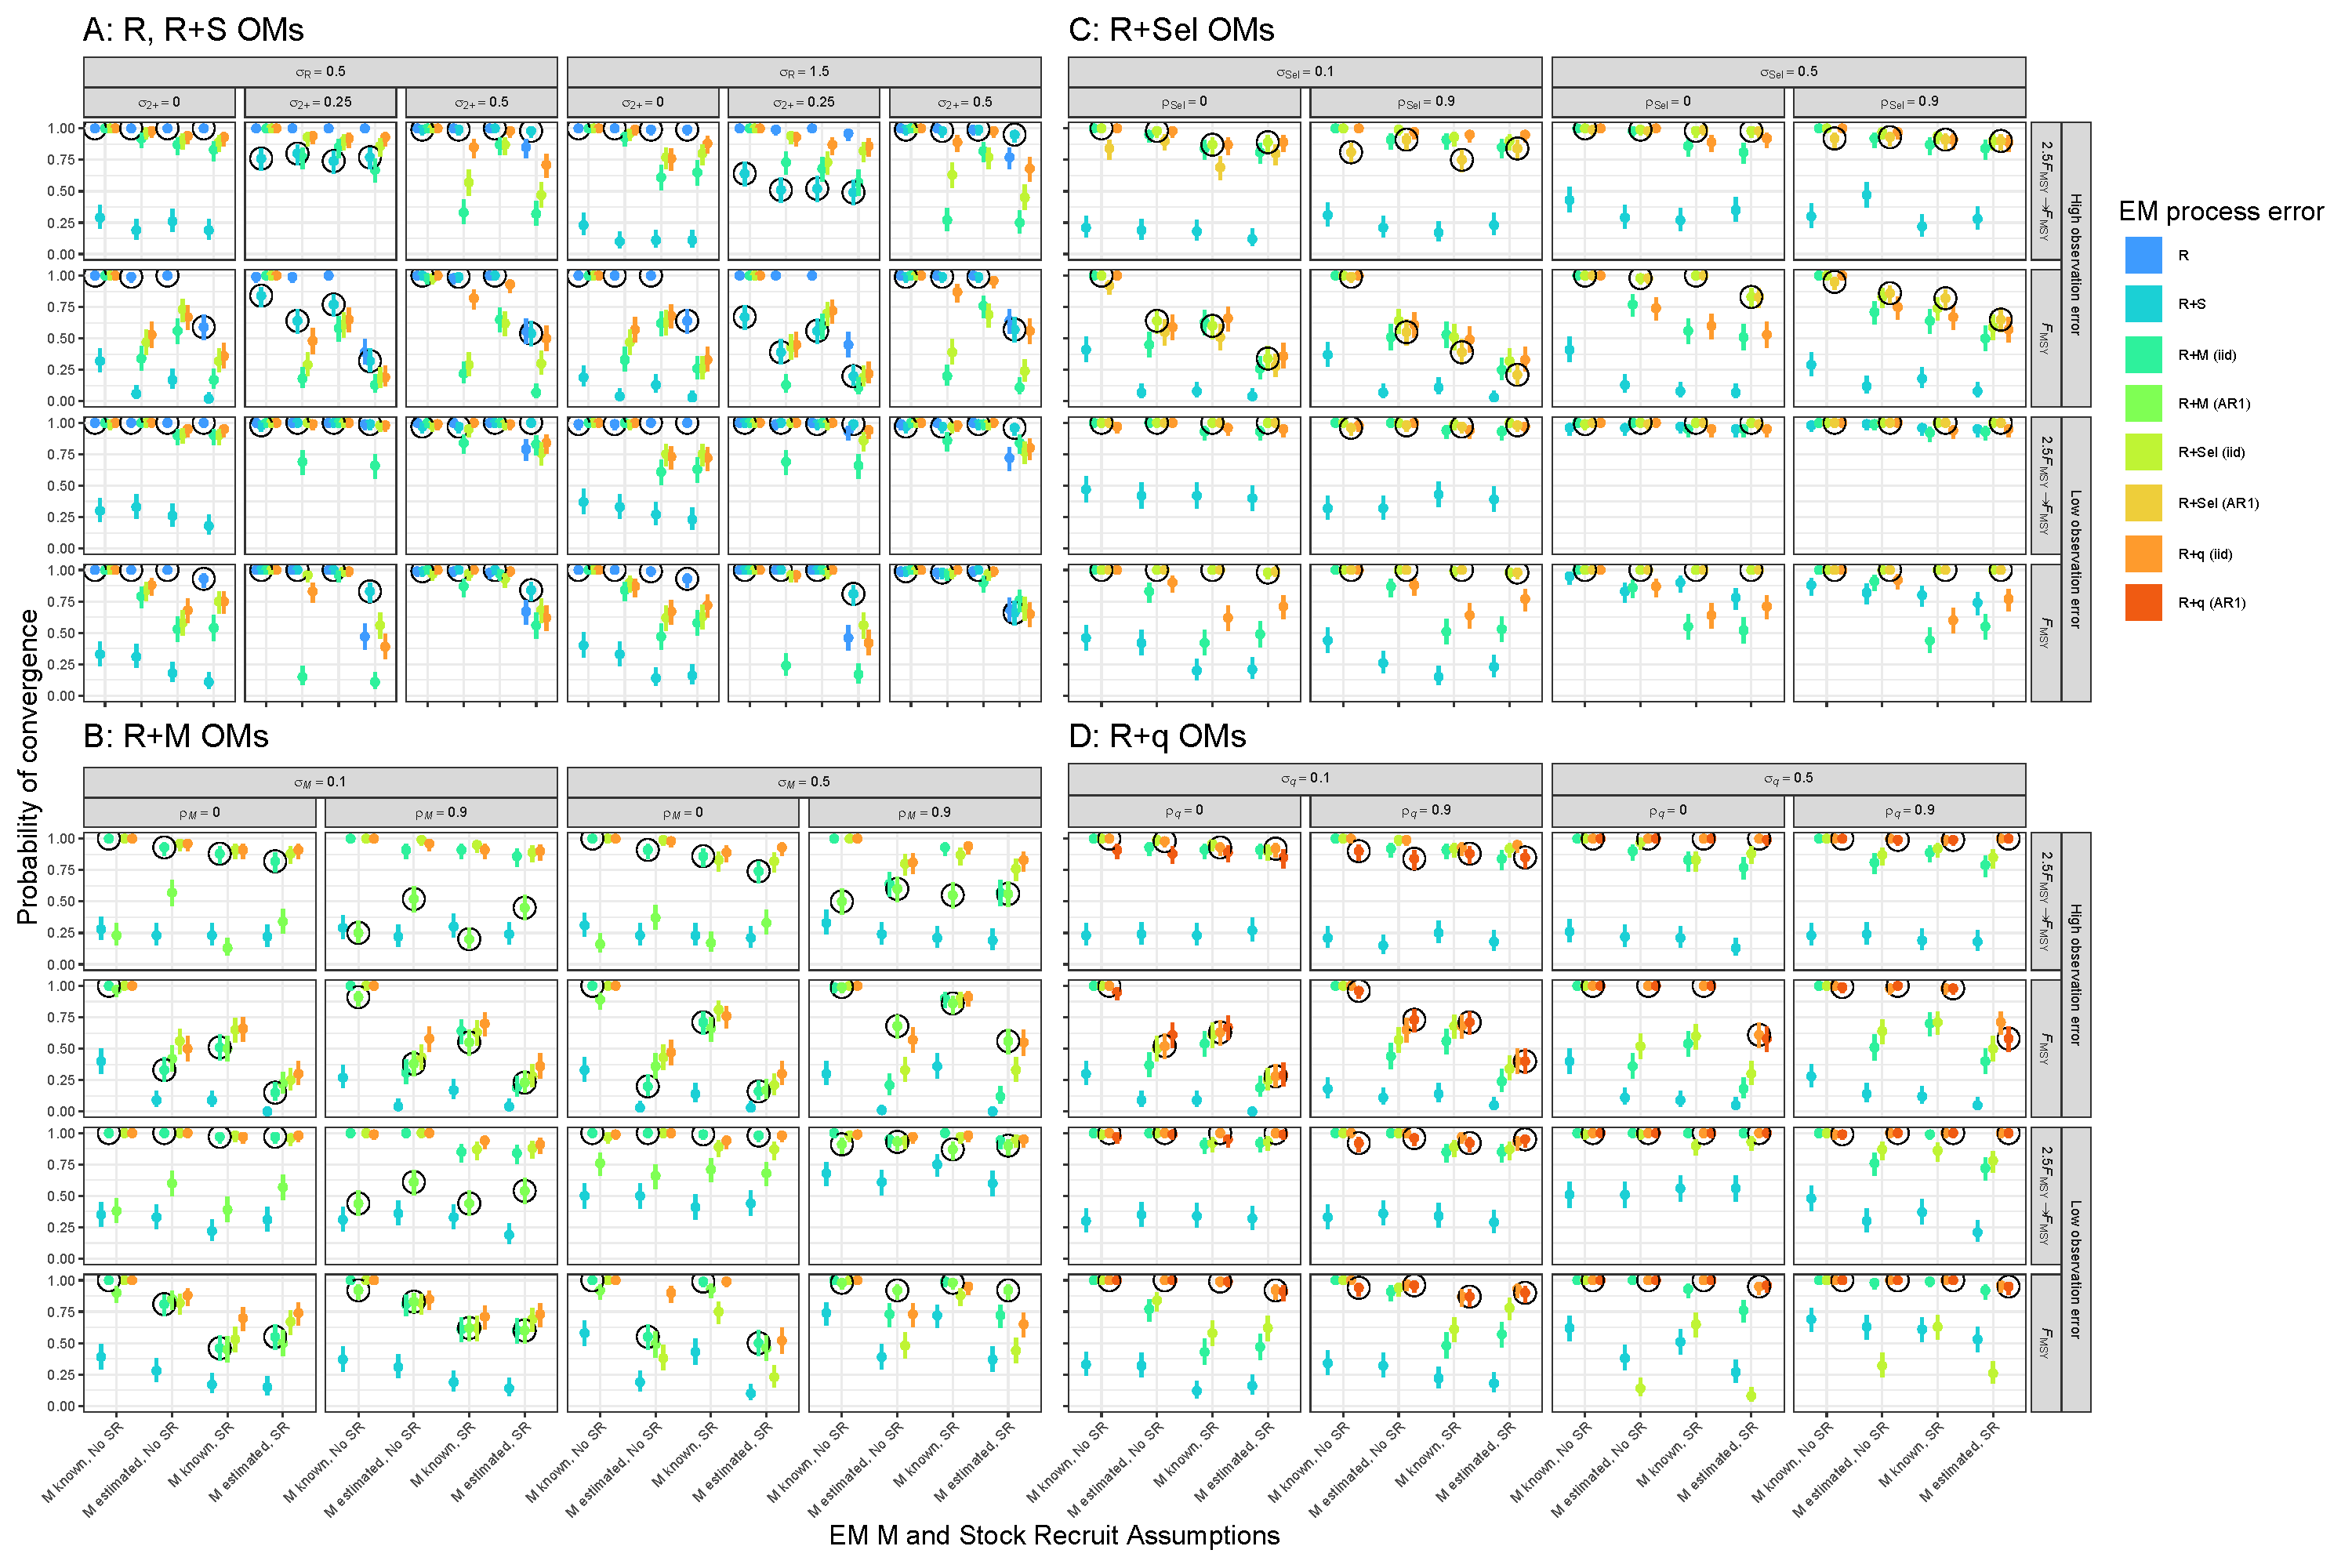
\includegraphics[width = 1.4\textwidth]{type_4_convergence_plots}
\DIFaddendFL \end{center}
\caption{\DIFdelbeginFL \DIFdelFL{Median relative error }\DIFdelendFL \DIFaddbeginFL \DIFaddFL{Estimated probability }\DIFaddendFL of \DIFdelbeginFL \DIFdelFL{terminal year recruitment }\DIFdelendFL \DIFaddbeginFL \DIFaddFL{fits providing hessian-based standard errors }\DIFaddendFL for \DIFdelbeginFL \DIFdelFL{estimating models fitted to data sets simulated with }\DIFdelendFL \DIFaddbeginFL \DIFaddFL{EMs assuming }\DIFaddendFL alternative process error \DIFdelbeginFL \DIFdelFL{structures: }\DIFdelendFL \DIFaddbeginFL \DIFaddFL{(colored points and lines), and median natural mortality (estimated or known) and Beverton-Holt stock-recruit relationships (estimated or not; along x-axis) when fitted to operating models that have }\DIFaddendFL R and R+S (A), R+Sel (B), R+M (C), or R+q (D) \DIFaddbeginFL \DIFaddFL{process error structures}\DIFaddendFL . Circled values indicate results where the EM process error structure matches that of the operating model and vertical lines represent 95\% confidence intervals.}\DIFdelbeginFL %DIFDELCMD < \label{R_rel_error}
%DIFDELCMD < %%%
\DIFdelendFL \DIFaddbeginFL \label{hessian_SE_convergence}
\DIFaddendFL \end{figure}
\end{landscape}

\begin{landscape}
\begin{figure}
\begin{center}
\DIFdelbeginFL %DIFDELCMD < 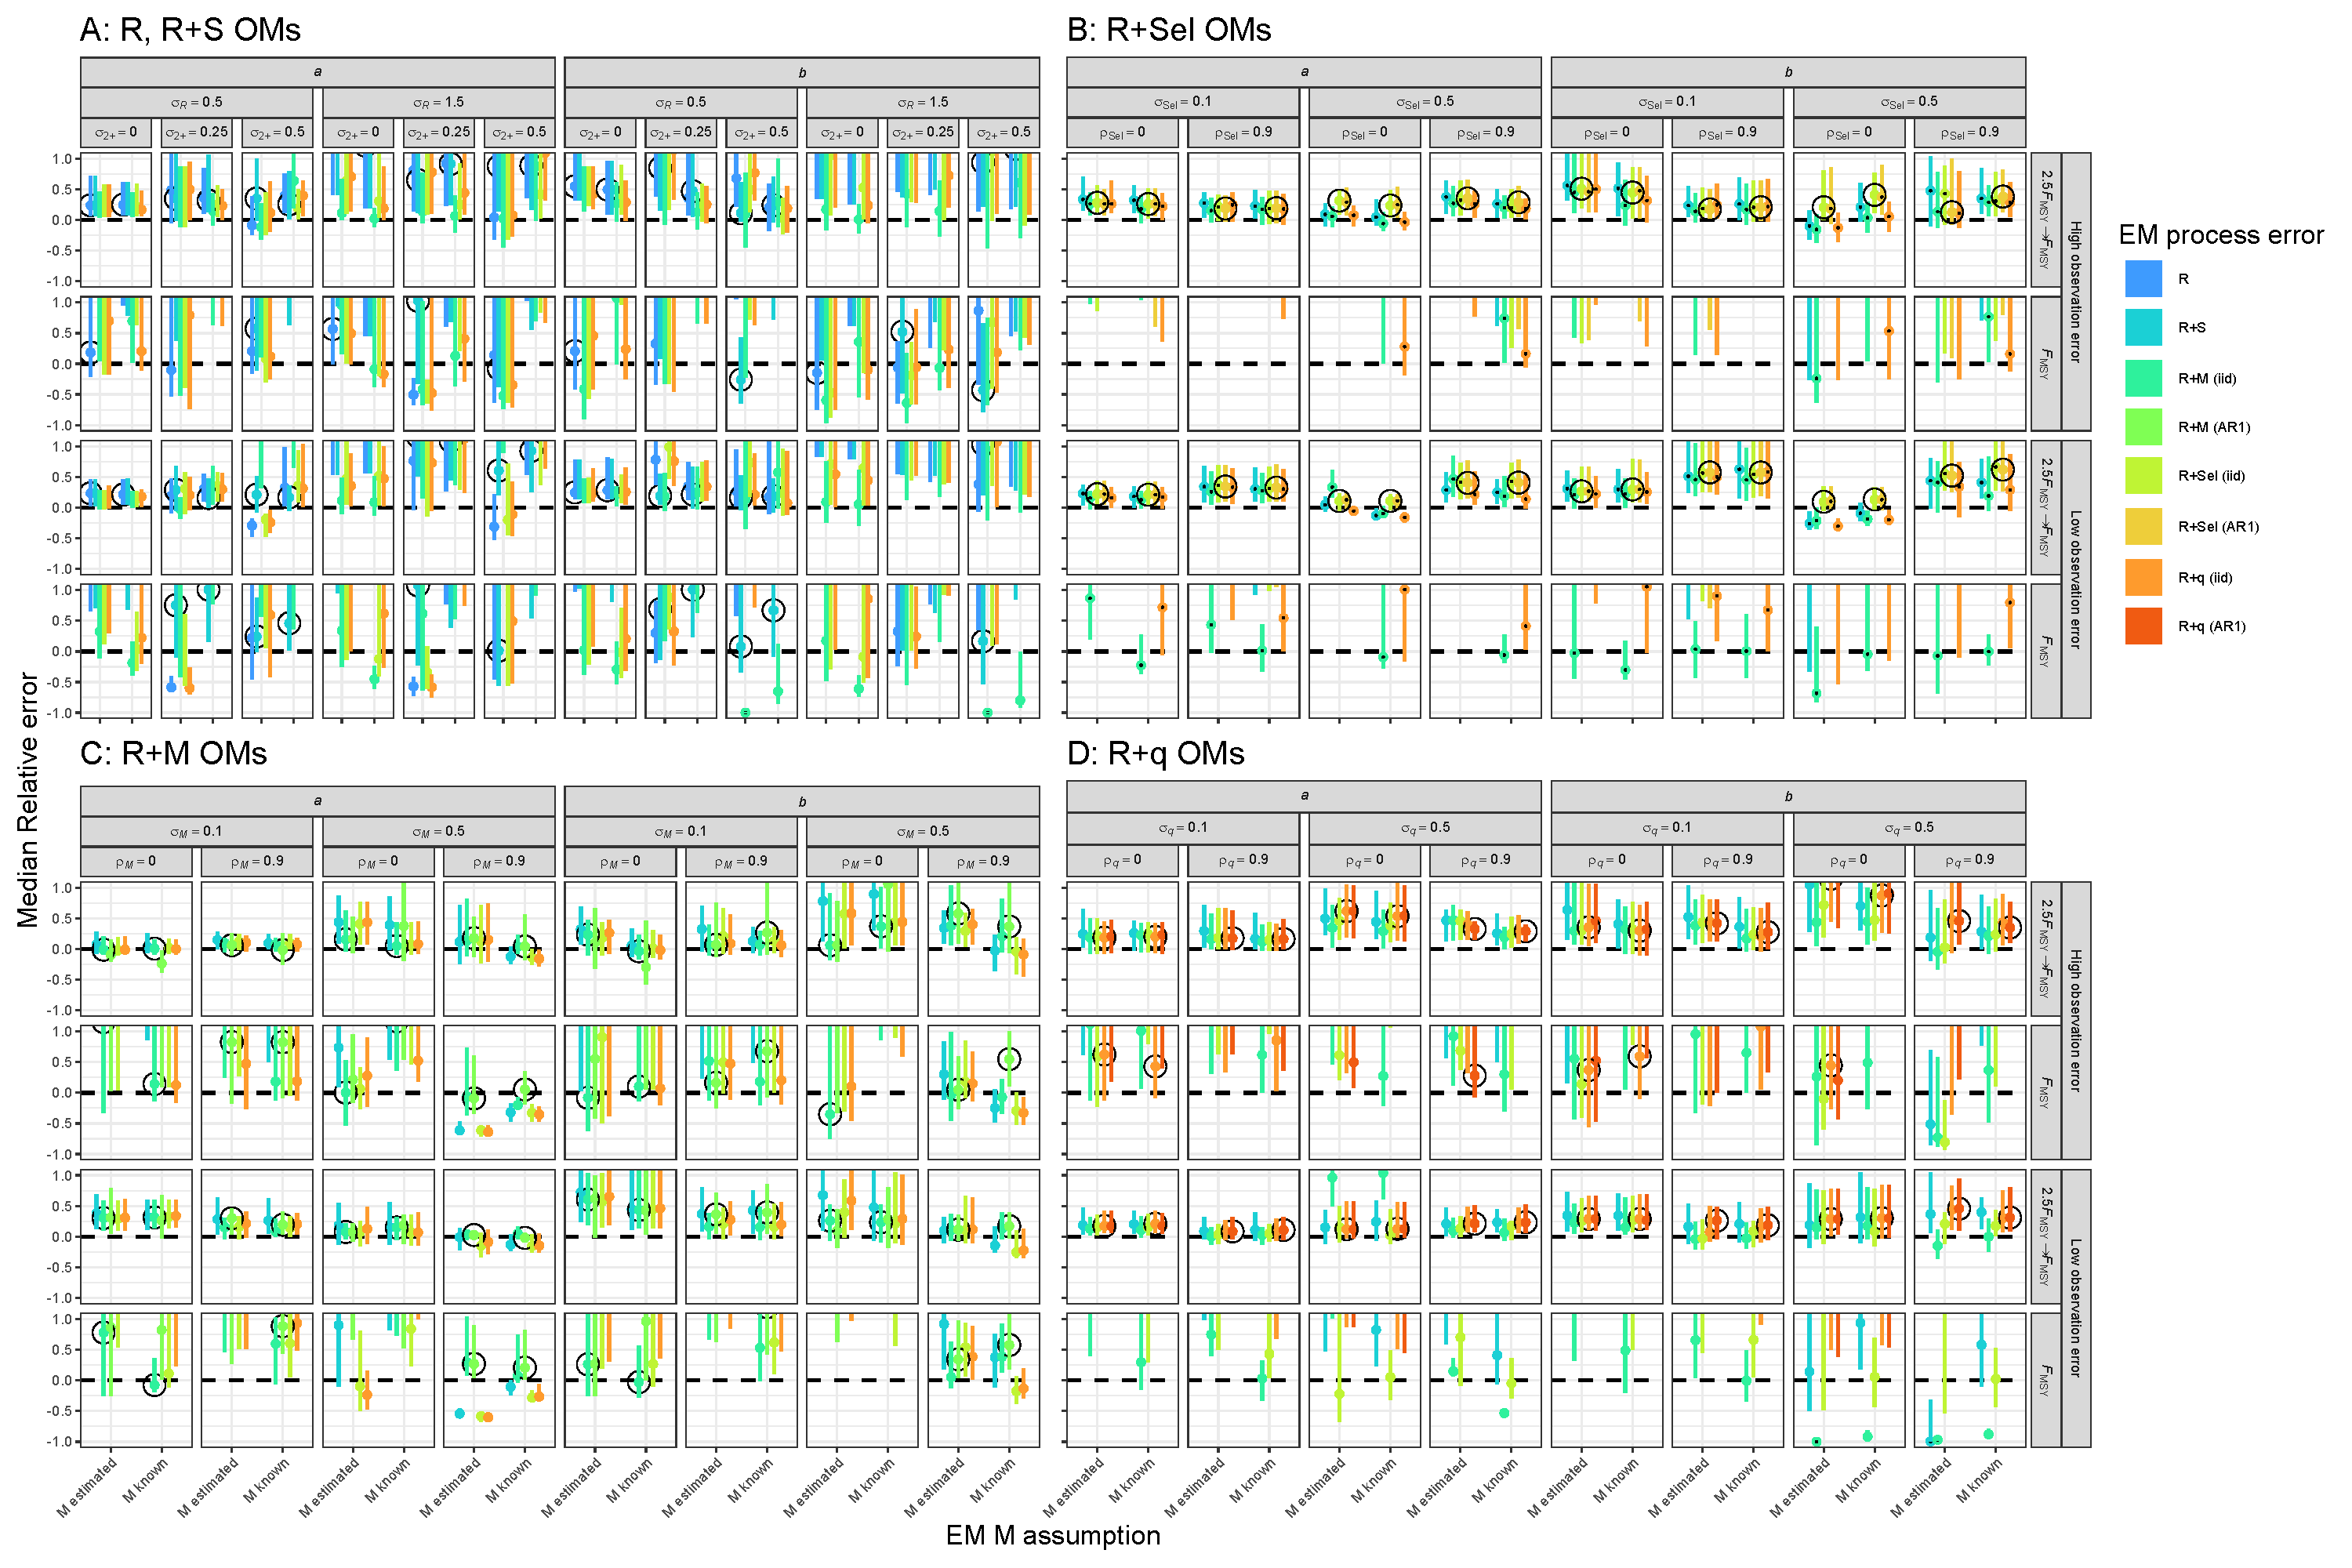
\includegraphics{sr_bias_plots}
%DIFDELCMD < %%%
\DIFdelendFL \DIFaddbeginFL 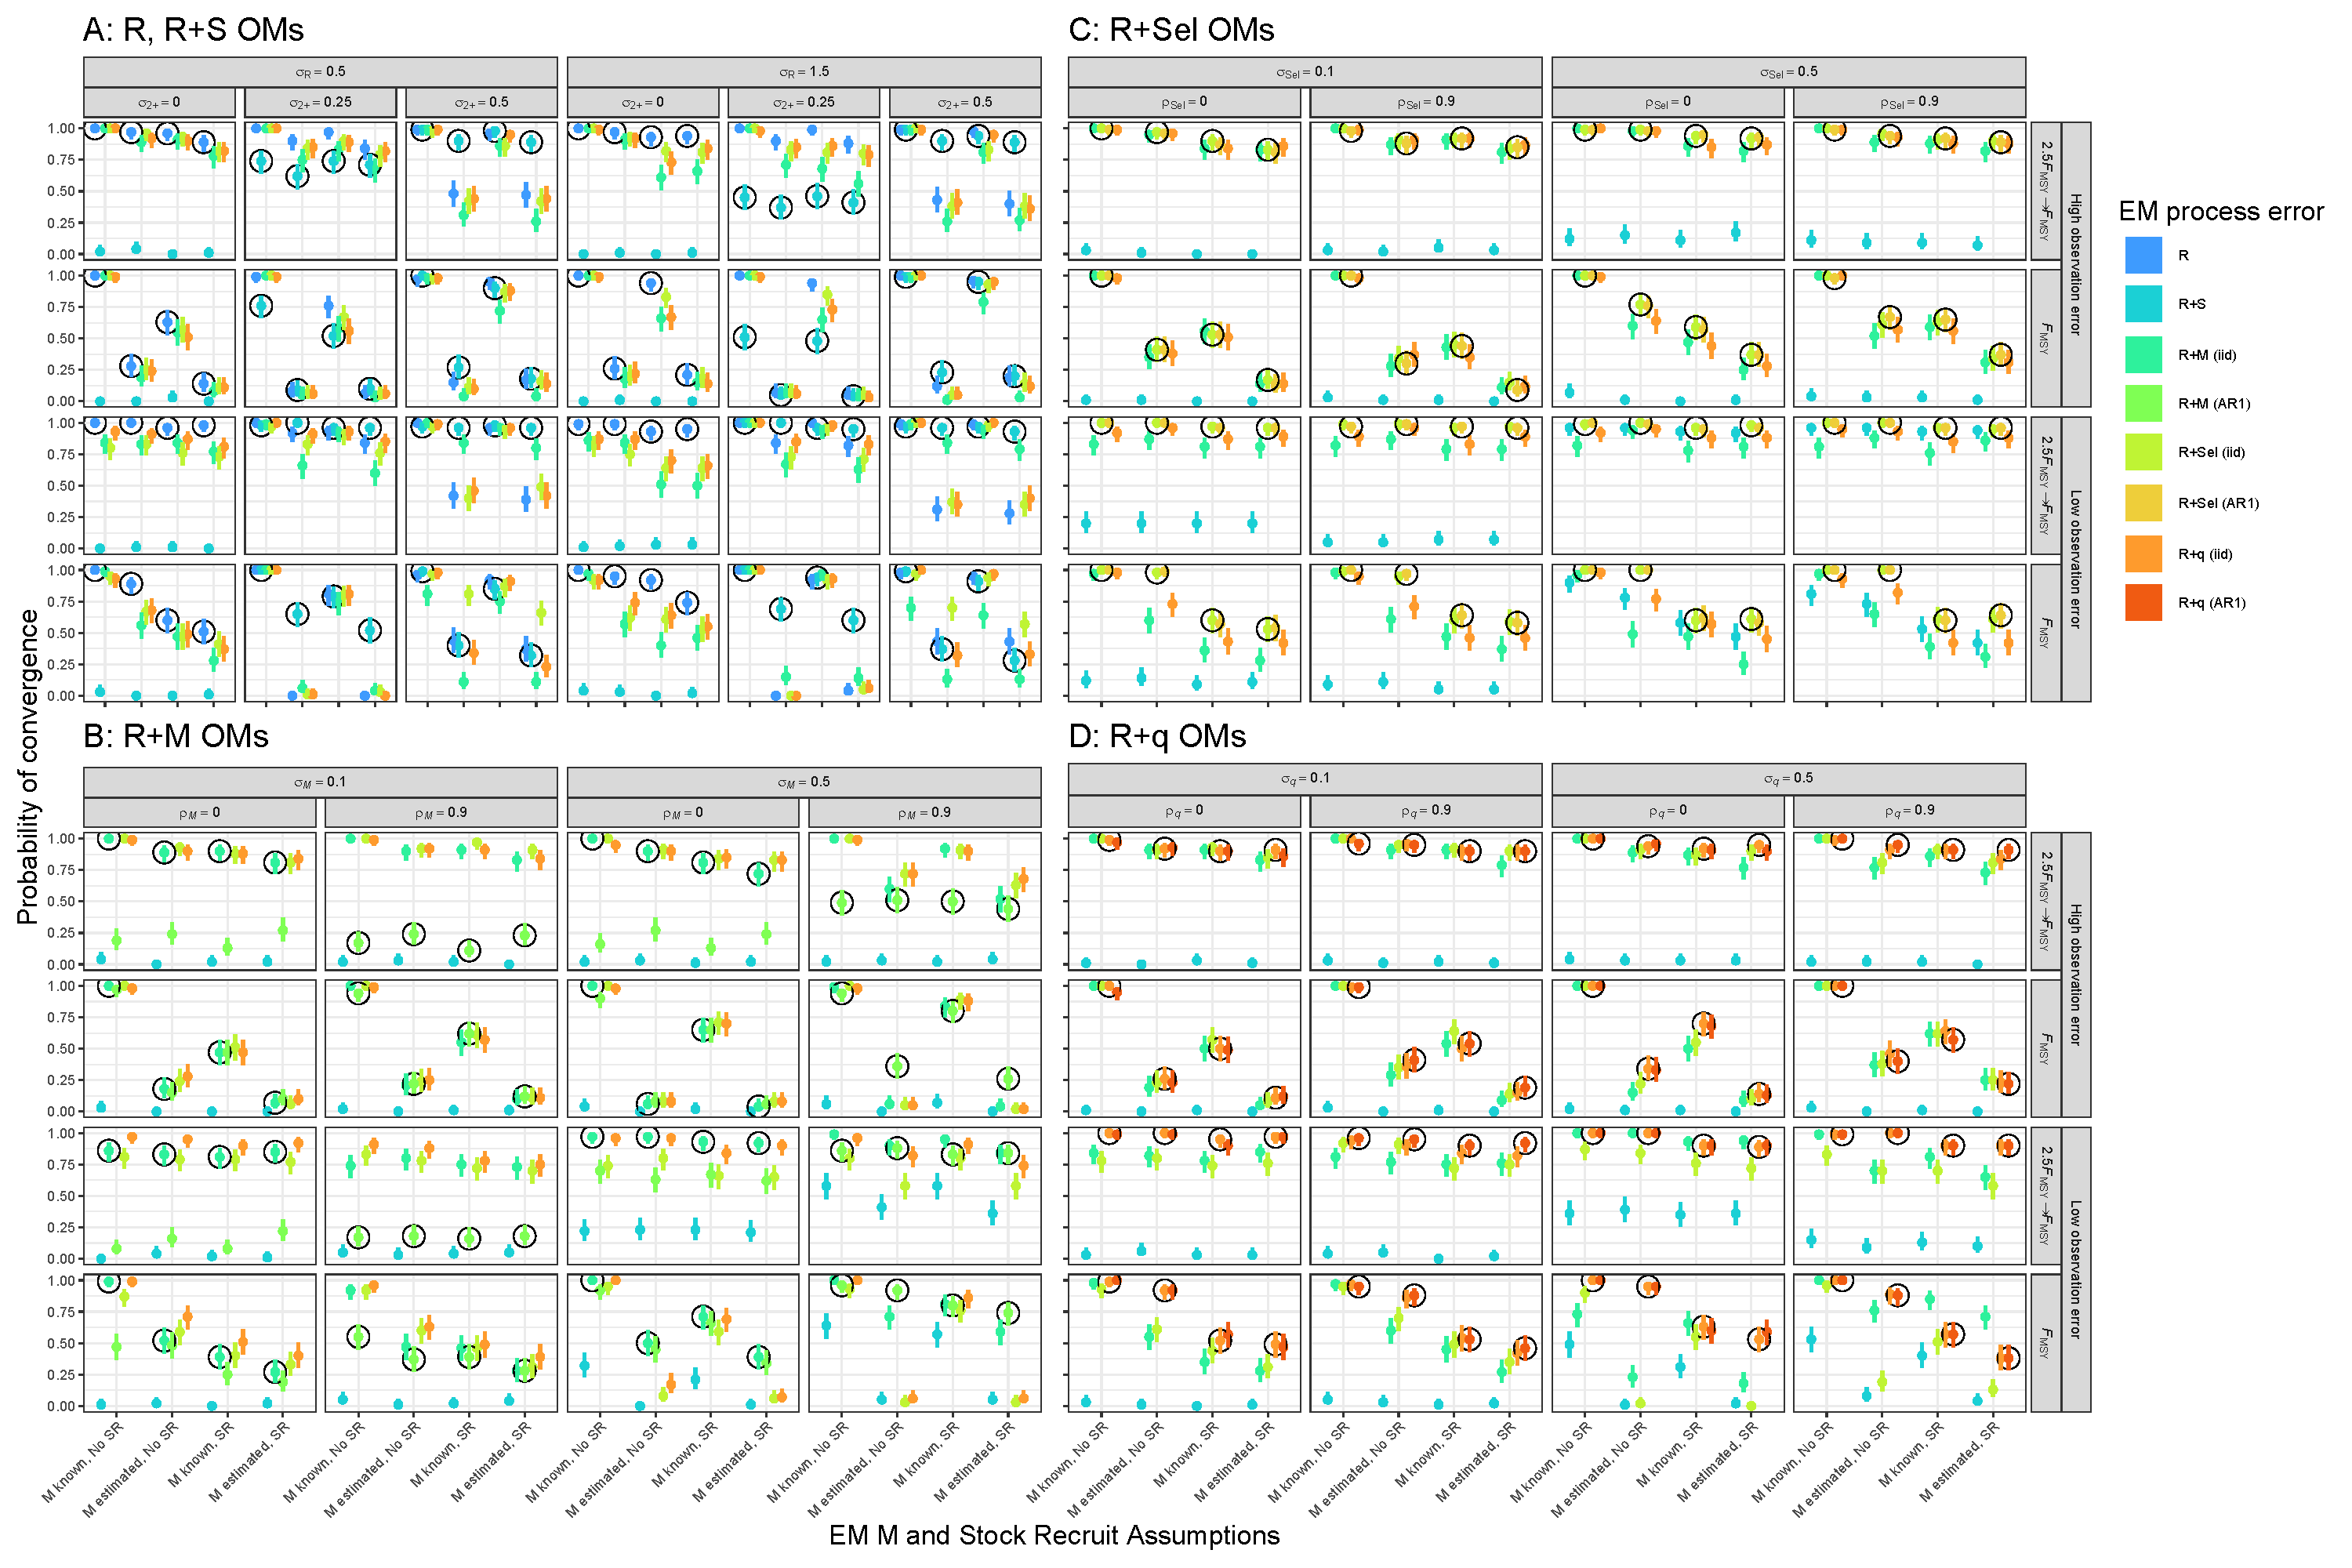
\includegraphics[width = 1.4\textwidth]{type_3_convergence_plots}
\DIFaddendFL \end{center}
\caption{\DIFdelbeginFL \DIFdelFL{Median relative error }\DIFdelendFL \DIFaddbeginFL \DIFaddFL{Probability }\DIFaddendFL of \DIFaddbeginFL \DIFaddFL{estimating models providing maximum absolute values of gradients less than $10^{-6}$ assuming alternative process error (colored points and lines), and median natural mortality (estimated or known) and }\DIFaddendFL Beverton-Holt stock-recruit \DIFdelbeginFL \DIFdelFL{parameters }\DIFdelendFL \DIFaddbeginFL \DIFaddFL{relationships }\DIFaddendFL (\DIFdelbeginFL \DIFdelFL{$a$ and $b$}\DIFdelendFL \DIFaddbeginFL \DIFaddFL{estimated or not; along x-axis}\DIFaddendFL ) \DIFdelbeginFL \DIFdelFL{for estimating models }\DIFdelendFL \DIFaddbeginFL \DIFaddFL{when }\DIFaddendFL fitted to \DIFdelbeginFL \DIFdelFL{data sets simulated with alternative process error structures: }\DIFdelendFL \DIFaddbeginFL \DIFaddFL{operating models that have }\DIFaddendFL R and R+S (A), R+Sel (B), R+M (C), or R+q (D) \DIFaddbeginFL \DIFaddFL{process error structures}\DIFaddendFL . Circled values indicate results where the EM process error structure matches that of the operating model and vertical lines represent 95\% confidence intervals.}\DIFdelbeginFL %DIFDELCMD < \label{SR_rel_error}
%DIFDELCMD < %%%
\DIFdelendFL \DIFaddbeginFL \label{gradient_convergence}
\DIFaddendFL \end{figure}
\end{landscape}

\DIFaddbegin \subsubsection*{\DIFadd{AIC for process error full
results}}\label{aic-for-process-error-full-results}
\addcontentsline{toc}{subsubsection}{\DIFadd{AIC for process error full results}}

\DIFadd{Marginal AIC accurately determined the correct process error assumptions
in EMs when data were generated from R and R+S OMs, regardless of
whether median natural mortality or a SRR was estimated (Figure
\ref{pe_aic}, A). Attempting to estimate median natural mortality or a
SRR separately had a negligible effect on the accuracy of determining
the correct process error assumption. When both were estimated, there
was a noticeable reduction in accuracy when OMs had a constant fishing
pressure, low observation error, and larger variability in recruitment
process errors.
}

\DIFadd{For R+M OMs, marginal AIC only accurately determined the correct process
error model and correlation structure when observation error was low and
variability in natural mortality process errors was high (Figures
\ref{pe_aic}, B). Of these OMs, estimating the median natural mortality
rate only reduced the accuracy of AIC when natural mortality process
errors were independent and fishing pressure was constant. For OMs with
poor model selection accuracy, AIC most frequently selected EMs with
process errors in catchability (R+q) or selectivity (R+Sel). Selection
of R+S EMs was generally unlikely.
}

\DIFadd{Marginal AIC most accurately determined the correct source of process
error and correlation structure for R+Sel OMs with low observation error
(Figures \ref{pe_aic}, C). When there was low variability in selectivity
process errors and high observation error, R+q or R+S EMs were more
likely to have the best AIC. Whether median natural morality or SRRs
were estimated appeared to have little effect on the performance of AIC.
}

\DIFadd{Marginal AIC most accurately determined the correct source of process
error and correlation structure for R+q OMs with high variability in
catchability process errors (Figures \ref{pe_aic},D). The R+q OMs with
low variability in catchability process errors and high observation
error had the least model selection accuracy. However, for these OMs,
the marginal AIC accurately determined the correct source of process
error (but not correlation structure) except when OMs assumed a constant
fishing pressure and EMs estimated both median natural morality and the
SRR.
}

\DIFaddend \begin{landscape}
\begin{figure}
\begin{center}
\DIFdelbeginFL %DIFDELCMD < 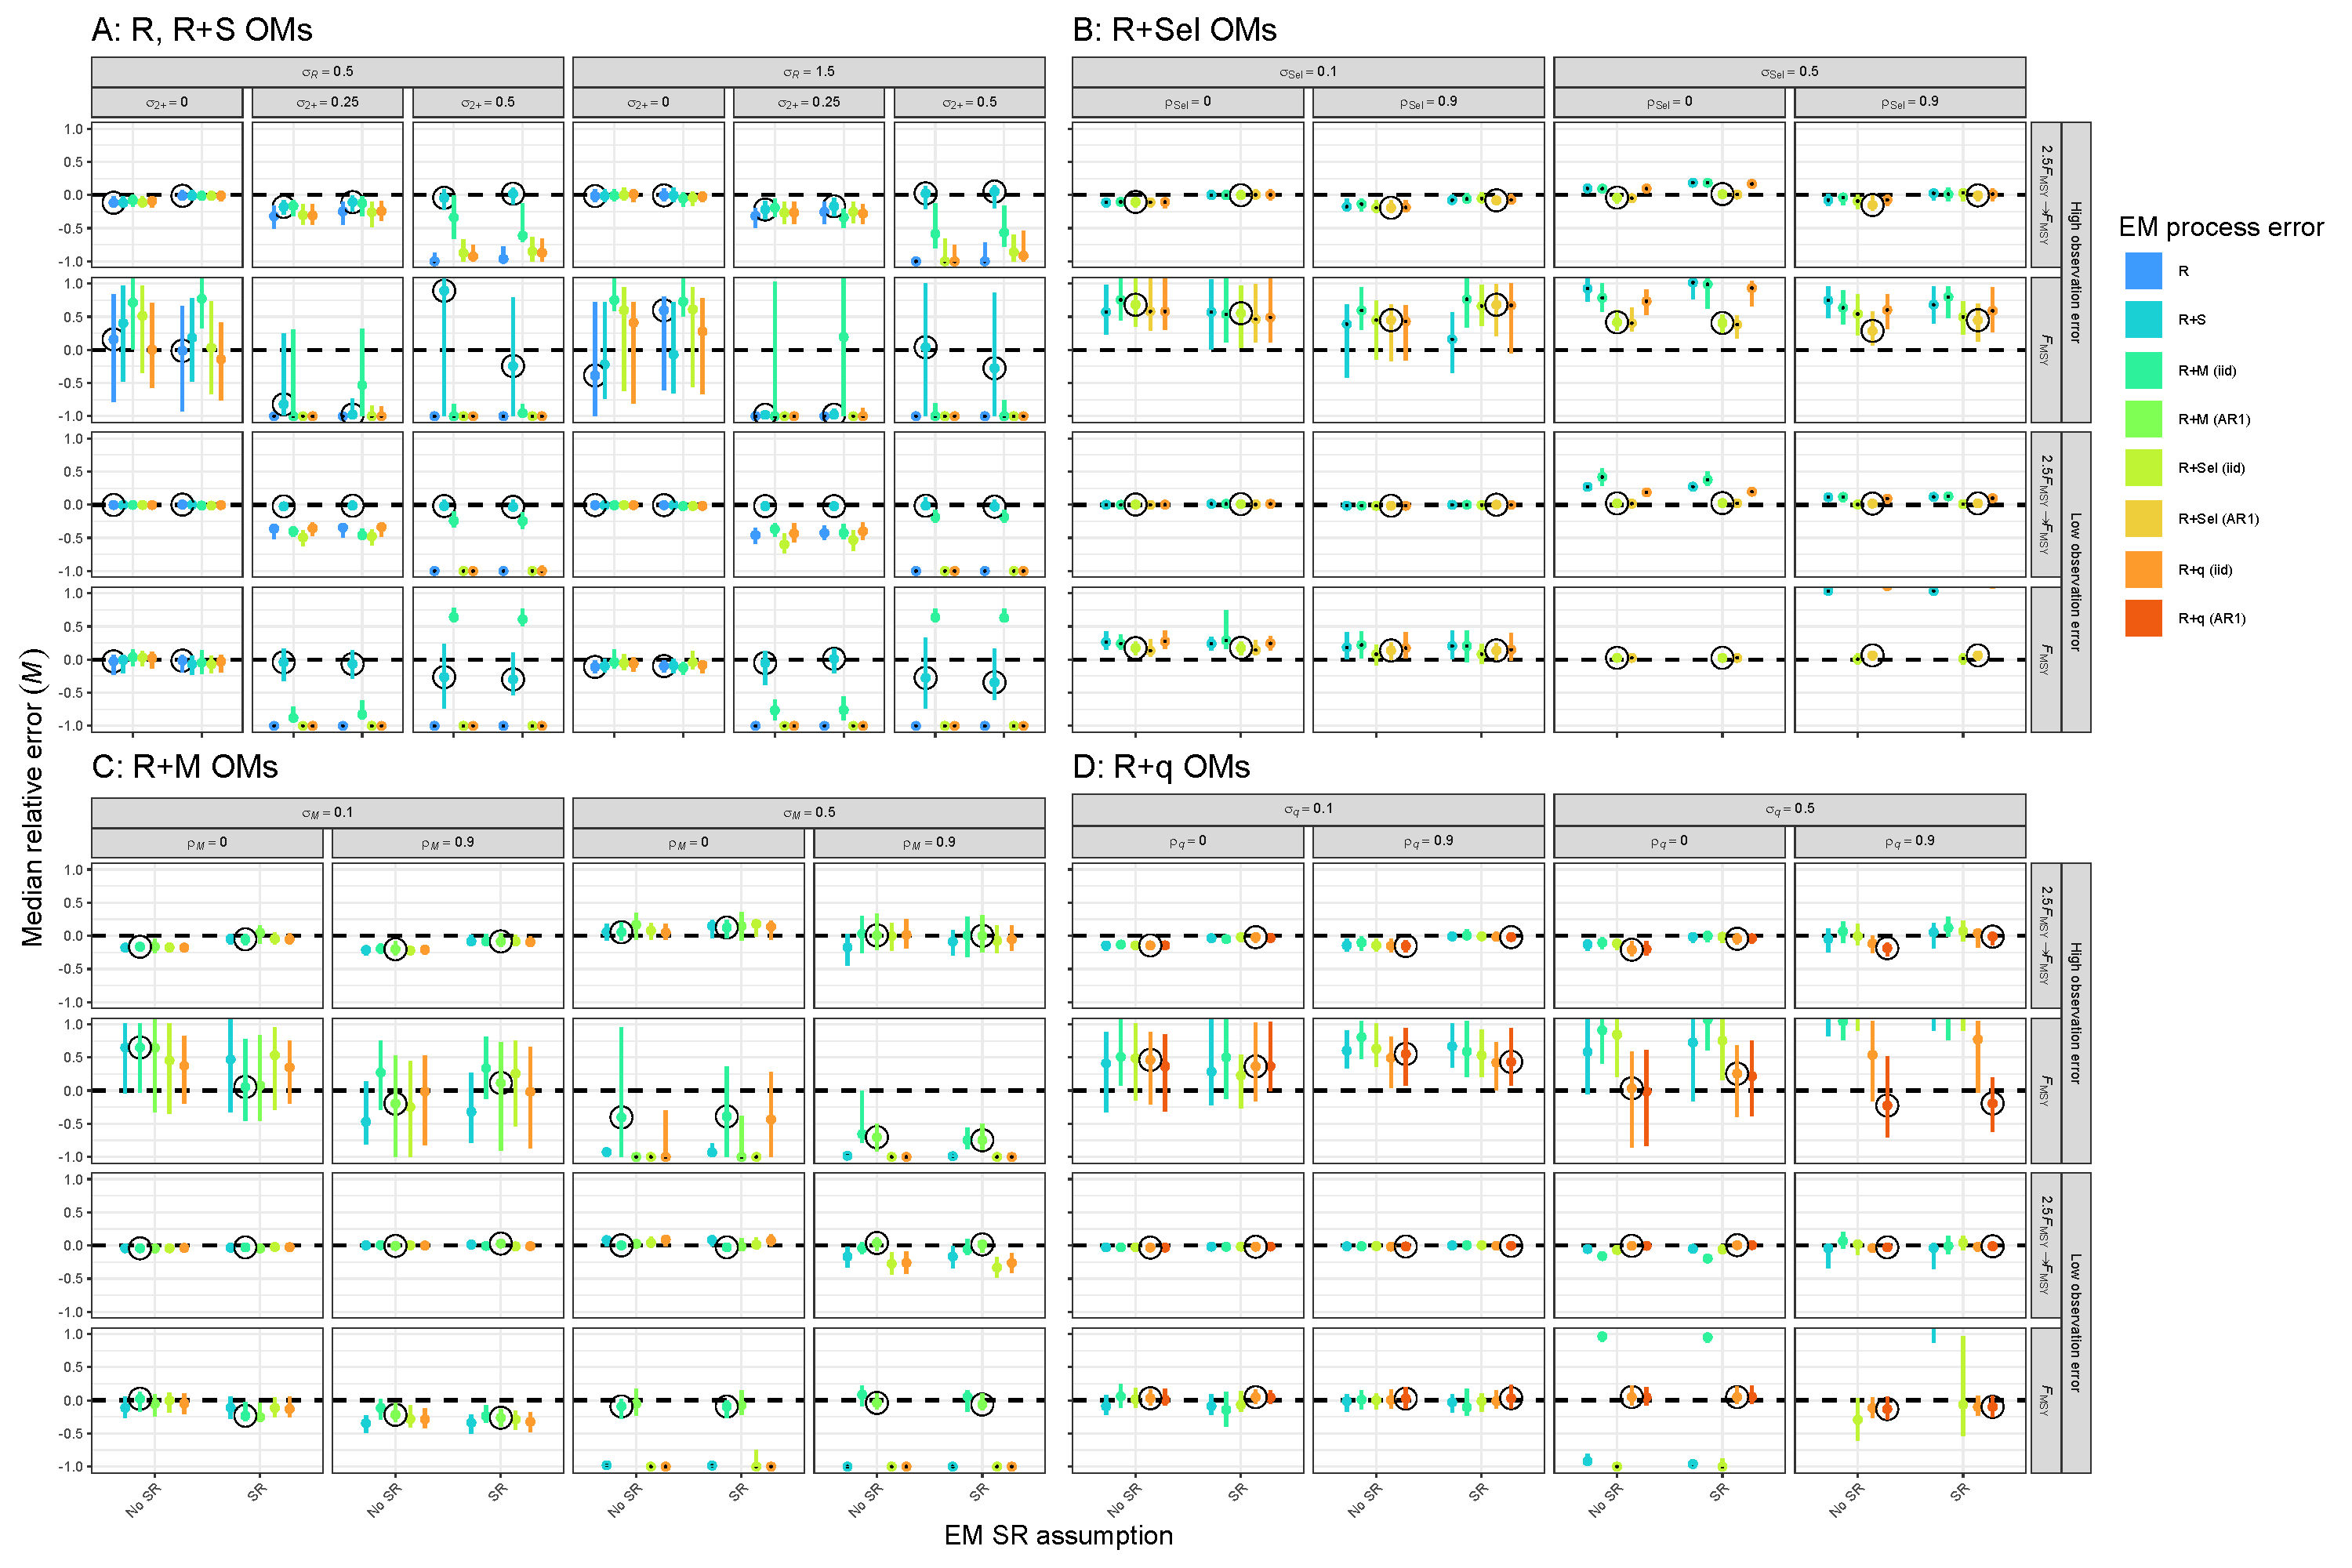
\includegraphics{M_bias_plots}
%DIFDELCMD < %%%
\DIFdelendFL \DIFaddbeginFL 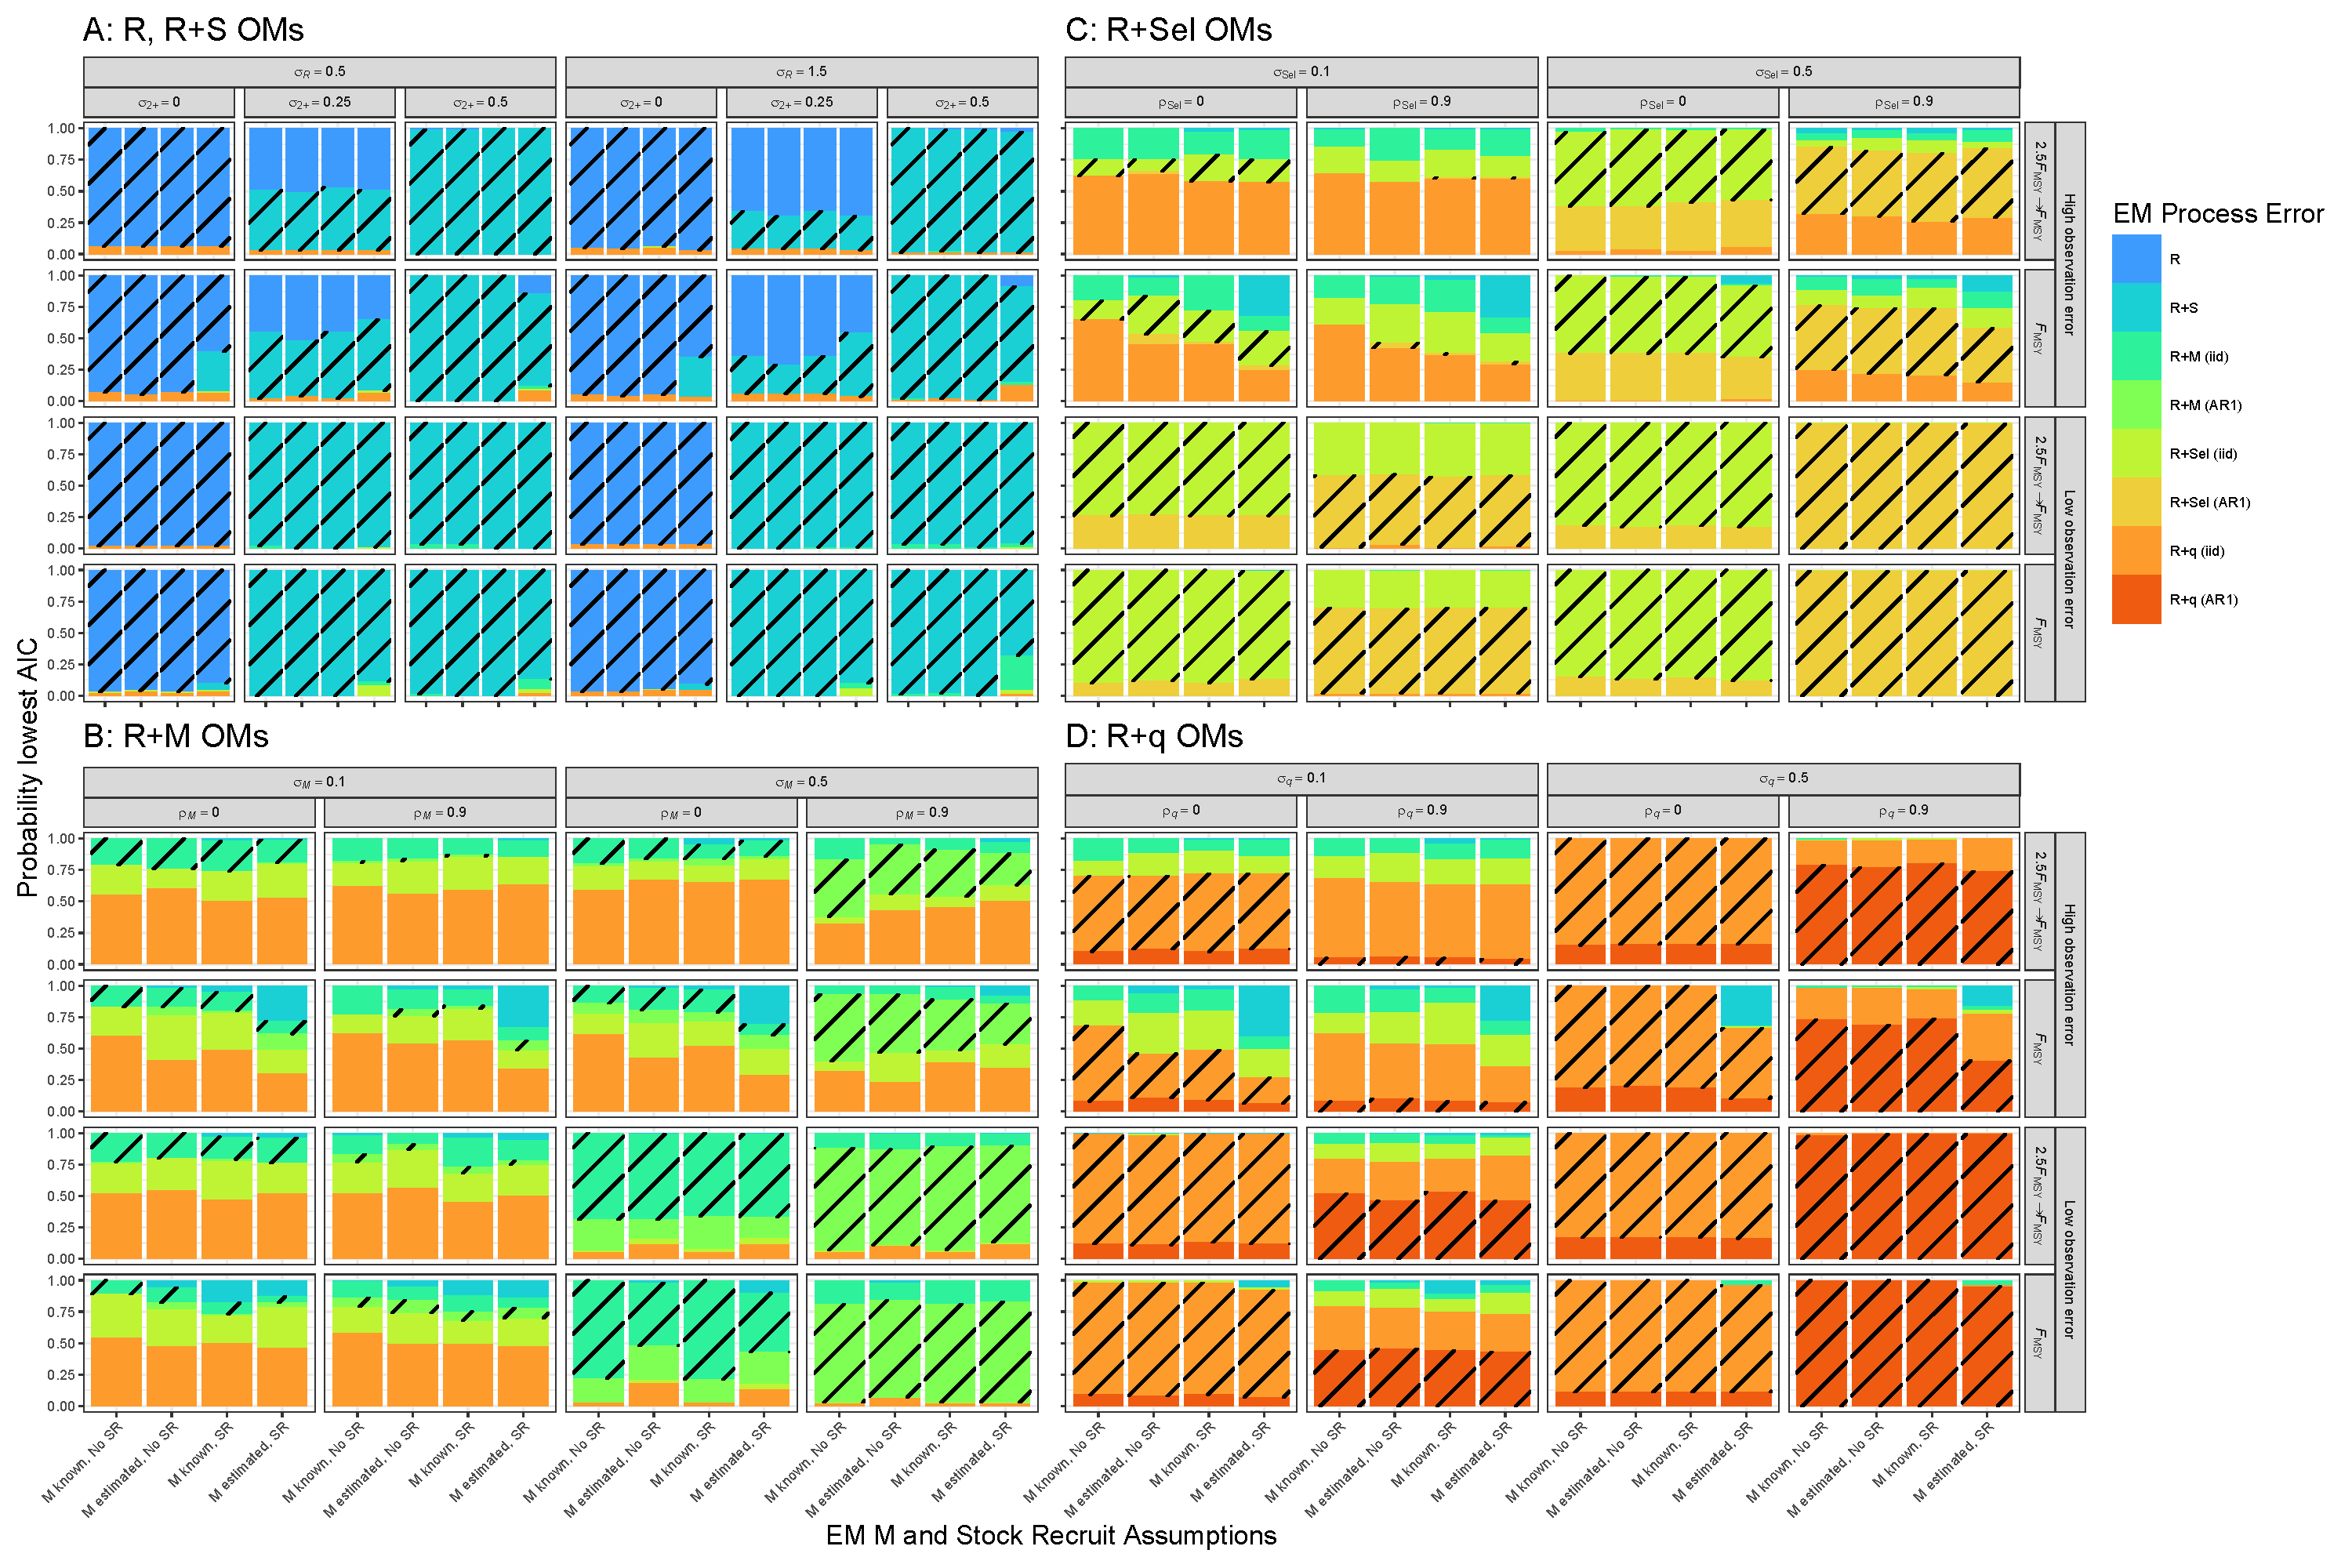
\includegraphics[width = 1.4\textwidth]{pe_aic_plots}
\DIFaddendFL \end{center}
\caption{\DIFdelbeginFL \DIFdelFL{Median relative error }\DIFdelendFL \DIFaddbeginFL \DIFaddFL{Estimated probability }\DIFaddendFL of \DIFdelbeginFL \DIFdelFL{median natural mortality }\DIFdelendFL \DIFaddbeginFL \DIFaddFL{lowest AIC }\DIFaddendFL for \DIFdelbeginFL \DIFdelFL{estimating models fitted to data sets simulated with }\DIFdelendFL \DIFaddbeginFL \DIFaddFL{EMs assuming }\DIFaddendFL alternative process error structures \DIFdelbeginFL \DIFdelFL{: }\DIFdelendFL \DIFaddbeginFL \DIFaddFL{(colored bars) conditional on alternative assumptions for median natural mortality (estimated or known) and Beverton-Holt stock-recruit relationships (estimated or not; along x-axis) when fitted to operating models that have }\DIFaddendFL R and R+S (A), R+Sel (B), R+M (C), or R+q (D) \DIFaddbeginFL \DIFaddFL{process error structures}\DIFaddendFL . \DIFdelbeginFL \DIFdelFL{Circled values }\DIFdelendFL \DIFaddbeginFL \DIFaddFL{Striped bars }\DIFaddendFL indicate results where the EM process error structure matches that of the operating model\DIFdelbeginFL \DIFdelFL{and vertical lines represent 95\% confidence intervals}\DIFdelendFL .}\DIFdelbeginFL %DIFDELCMD < \label{M_rel_error}
%DIFDELCMD < %%%
\DIFdelendFL \DIFaddbeginFL \label{pe_aic}
\DIFaddendFL \end{figure}
\end{landscape}

\DIFaddbegin \subsubsection*{\DIFadd{AIC for stock-recruit relationship full
results}}\label{aic-for-stock-recruit-relationship-full-results}
\addcontentsline{toc}{subsubsection}{\DIFadd{AIC for stock-recruit relationship
full results}}

\DIFadd{For each EM and OM combination, we fit logistic regression models to the
indicator of Beverton-Holt models having lower AIC as a function of the
log-standard deviation of the true log(SSB) (similar to the log of the
coefficient of variation for SSB) since simulations with realized SSB
producing low and high recruitment would have larger variation in
realized SSB.
}

\DIFadd{Our comparisons of model performance conditioned on assuming the true
process error configuration is known (EM and OM process error types
match) and we focus on results where the EMs assume median natural
mortality is known because there was little difference in results when
the EMs estimated this parameter. Broadly, we found generally poor
accuracy of AIC in selecting models assuming a Beverton-Holt SRR over
the null model without an SRR for all OMs. However, we also found
increased accuracy of AIC in determining the Beverton-Holt SRR when the
simulated population exhibited greater variation in spawning biomass for
nearly every OM (Figure \ref{sr_aic}).
}

\DIFadd{With R and R+S process error assumptions, probability of lowest AIC for
the B-H SRR as a function of SSB variability were greatest for OMs with
contrast in fishing pressure and lower process variability in
recruitment (Figure \ref{sr_aic}, A). The largest variation in SSB
occurred in OMs with larger recruitment variability (\(\sigma_R = 1.5\);
Figure \ref{sr_aic}, A, right column group), but the same high AIC
accuracy was achieved for OMs with lower recruitment variability at
lower levels of SSB variation. The level of observation error had little
effect on AIC accuracy.
}

\DIFadd{For R+M OMs, probability of lowest AIC for the Beverton-Holt SRR
increased steeply with variation in SSB whether it was induced by
contrast in fishing or variation in natural mortality process error.
(Figure \ref{sr_aic}, B). There was little difference in AIC accuracy
whether the natural mortality process errors were correleted and,
similar to R+S OMs, there was also little effect due to level of
observation error.
}

\DIFadd{For R+Sel OMs, contrast in fishing pressure over time was the primary
source of variation in SSB and these are the OMs where AIC accuracy for
the Beverton-Holt SRR was greatest (Figure \ref{sr_aic}, C). There was
little effect of variability or correlation of selectivity process
errors or the level of observation error on AIC accuracy.
}

\DIFadd{Like the R+Sel OMs, the greatest accuracy for AIC in selecting the
Beverton-Holt SRR occurred for R+q OMs where there was contrast in
fishing pressure over time which is also where there was the greatest
variation in SSB (Figure \ref{sr_aic}, D). There was also little effect
of variability or correlation of catchability process errors or the
level of observation error on AIC accuracy.
}

\DIFaddend \begin{landscape}
\begin{figure}
\begin{center}
\DIFdelbeginFL %DIFDELCMD < 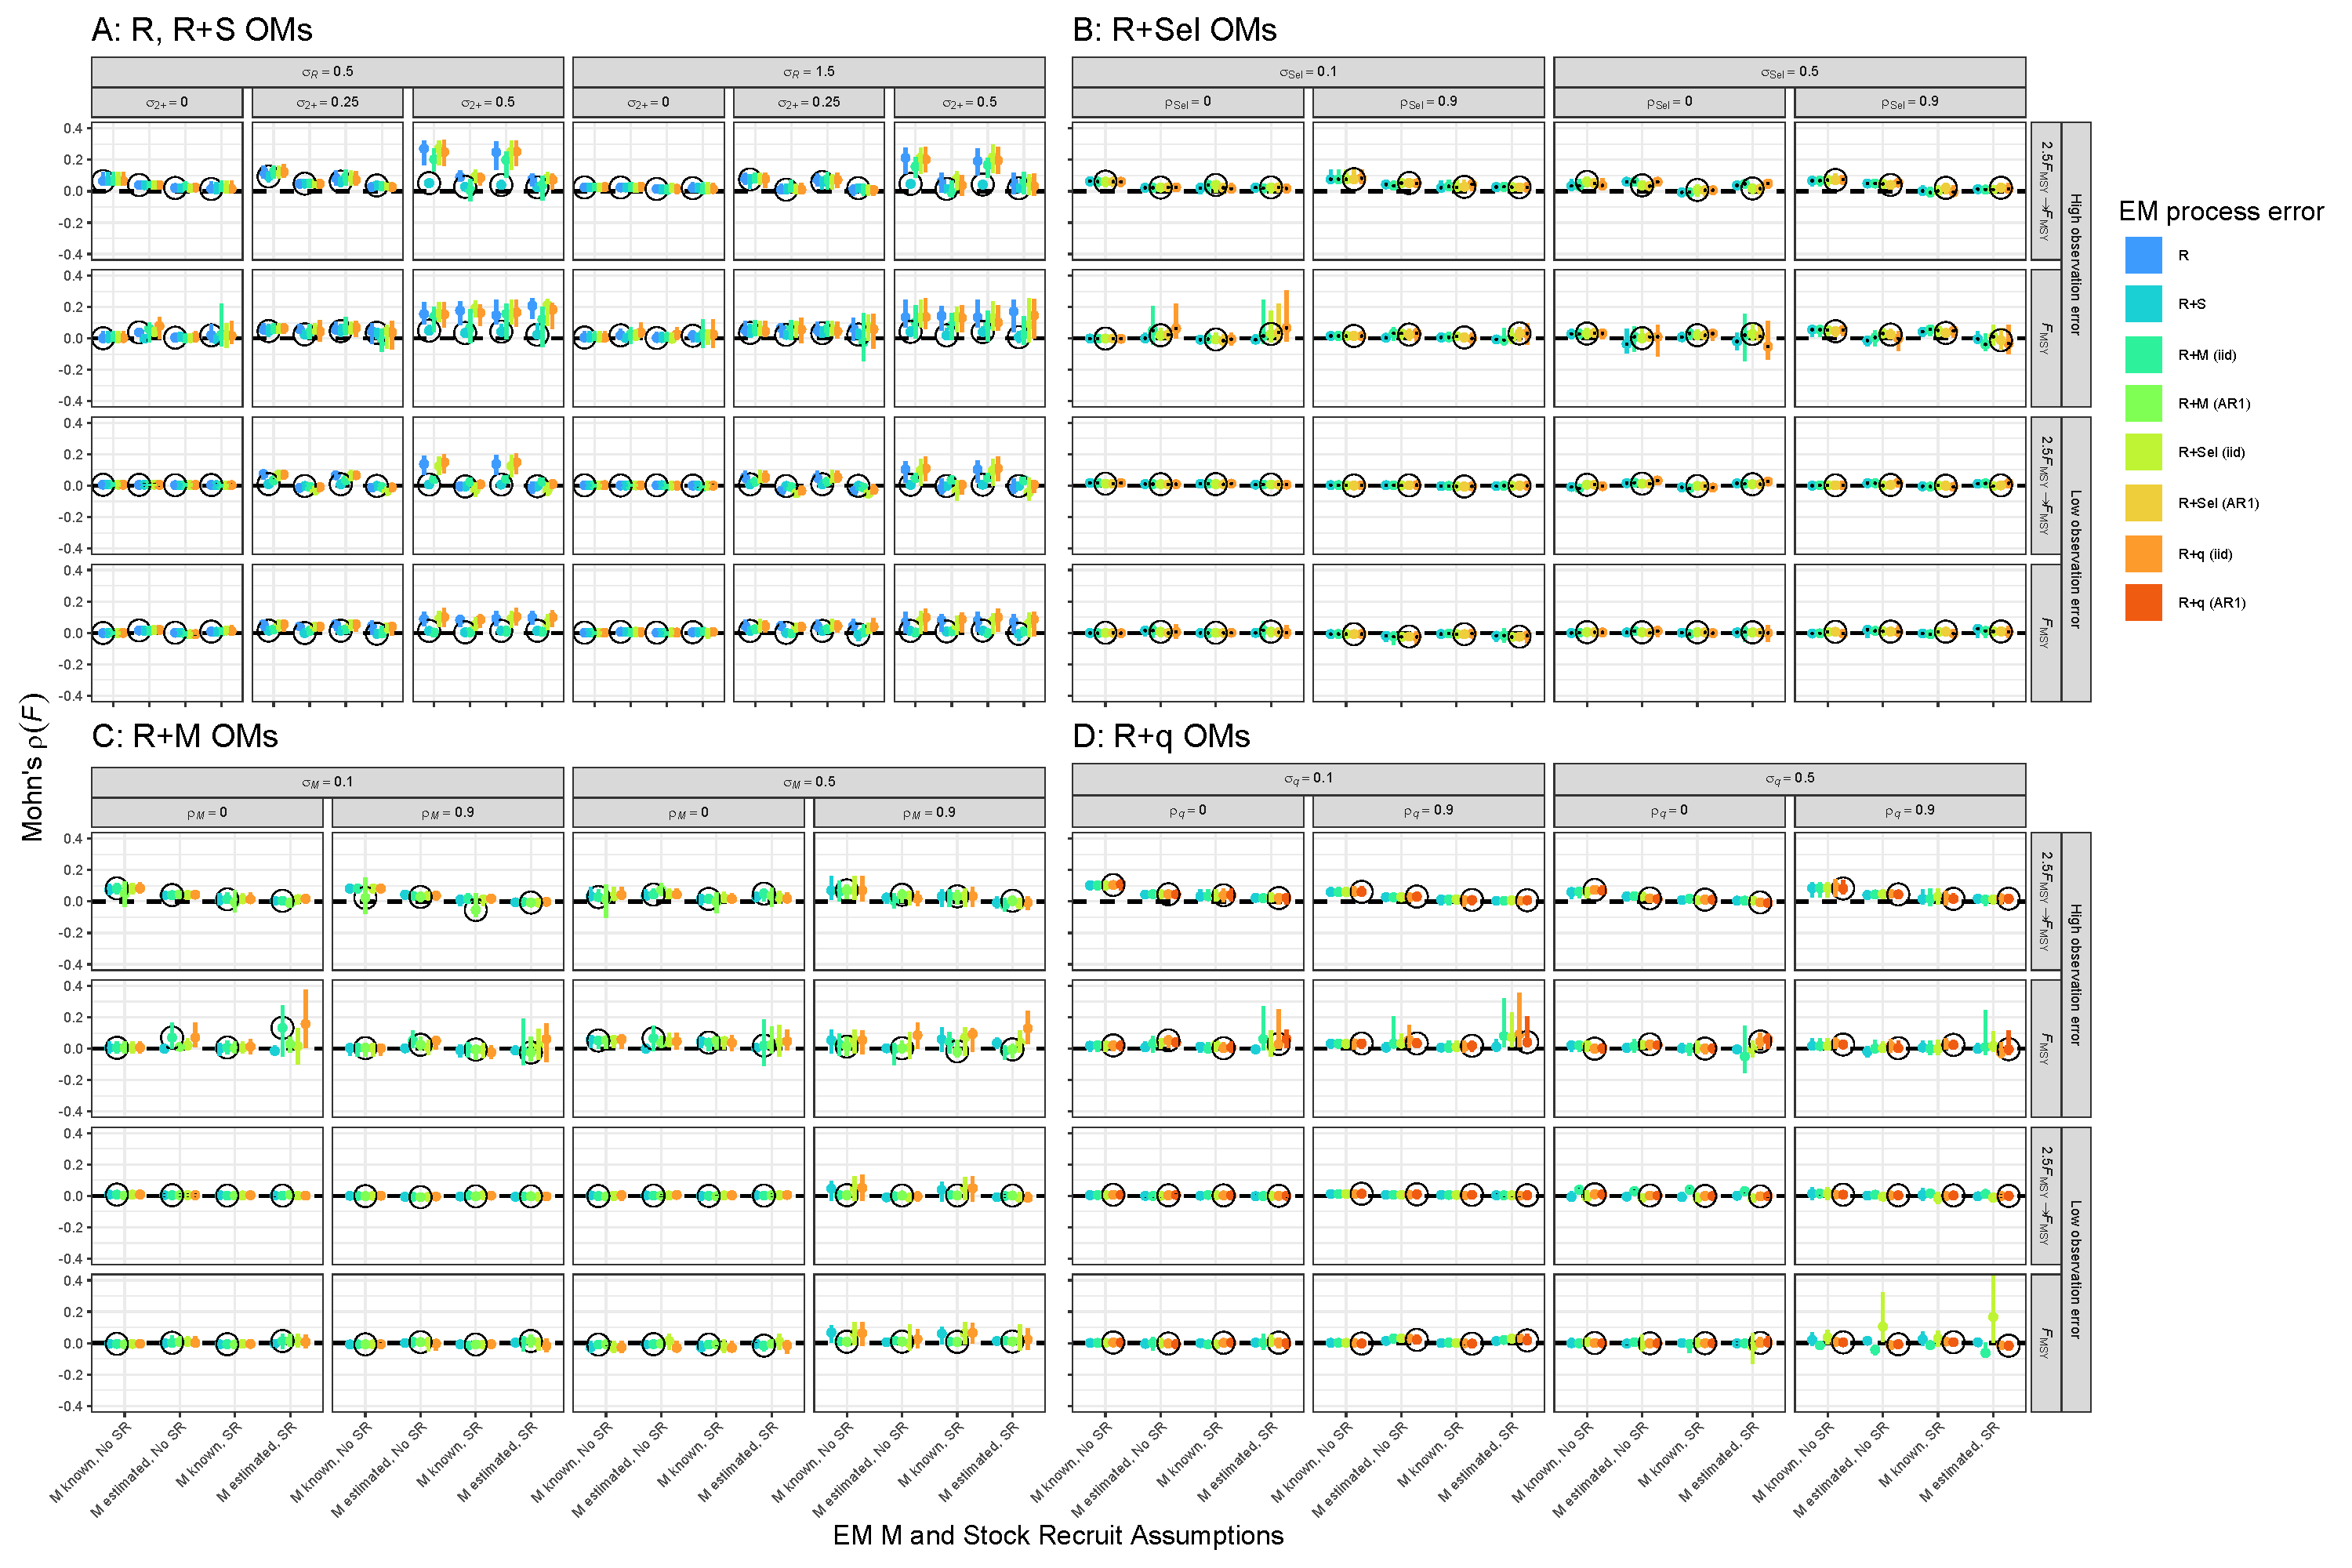
\includegraphics{mohns_rho_F_plots}
%DIFDELCMD < %%%
\DIFdelendFL \DIFaddbeginFL 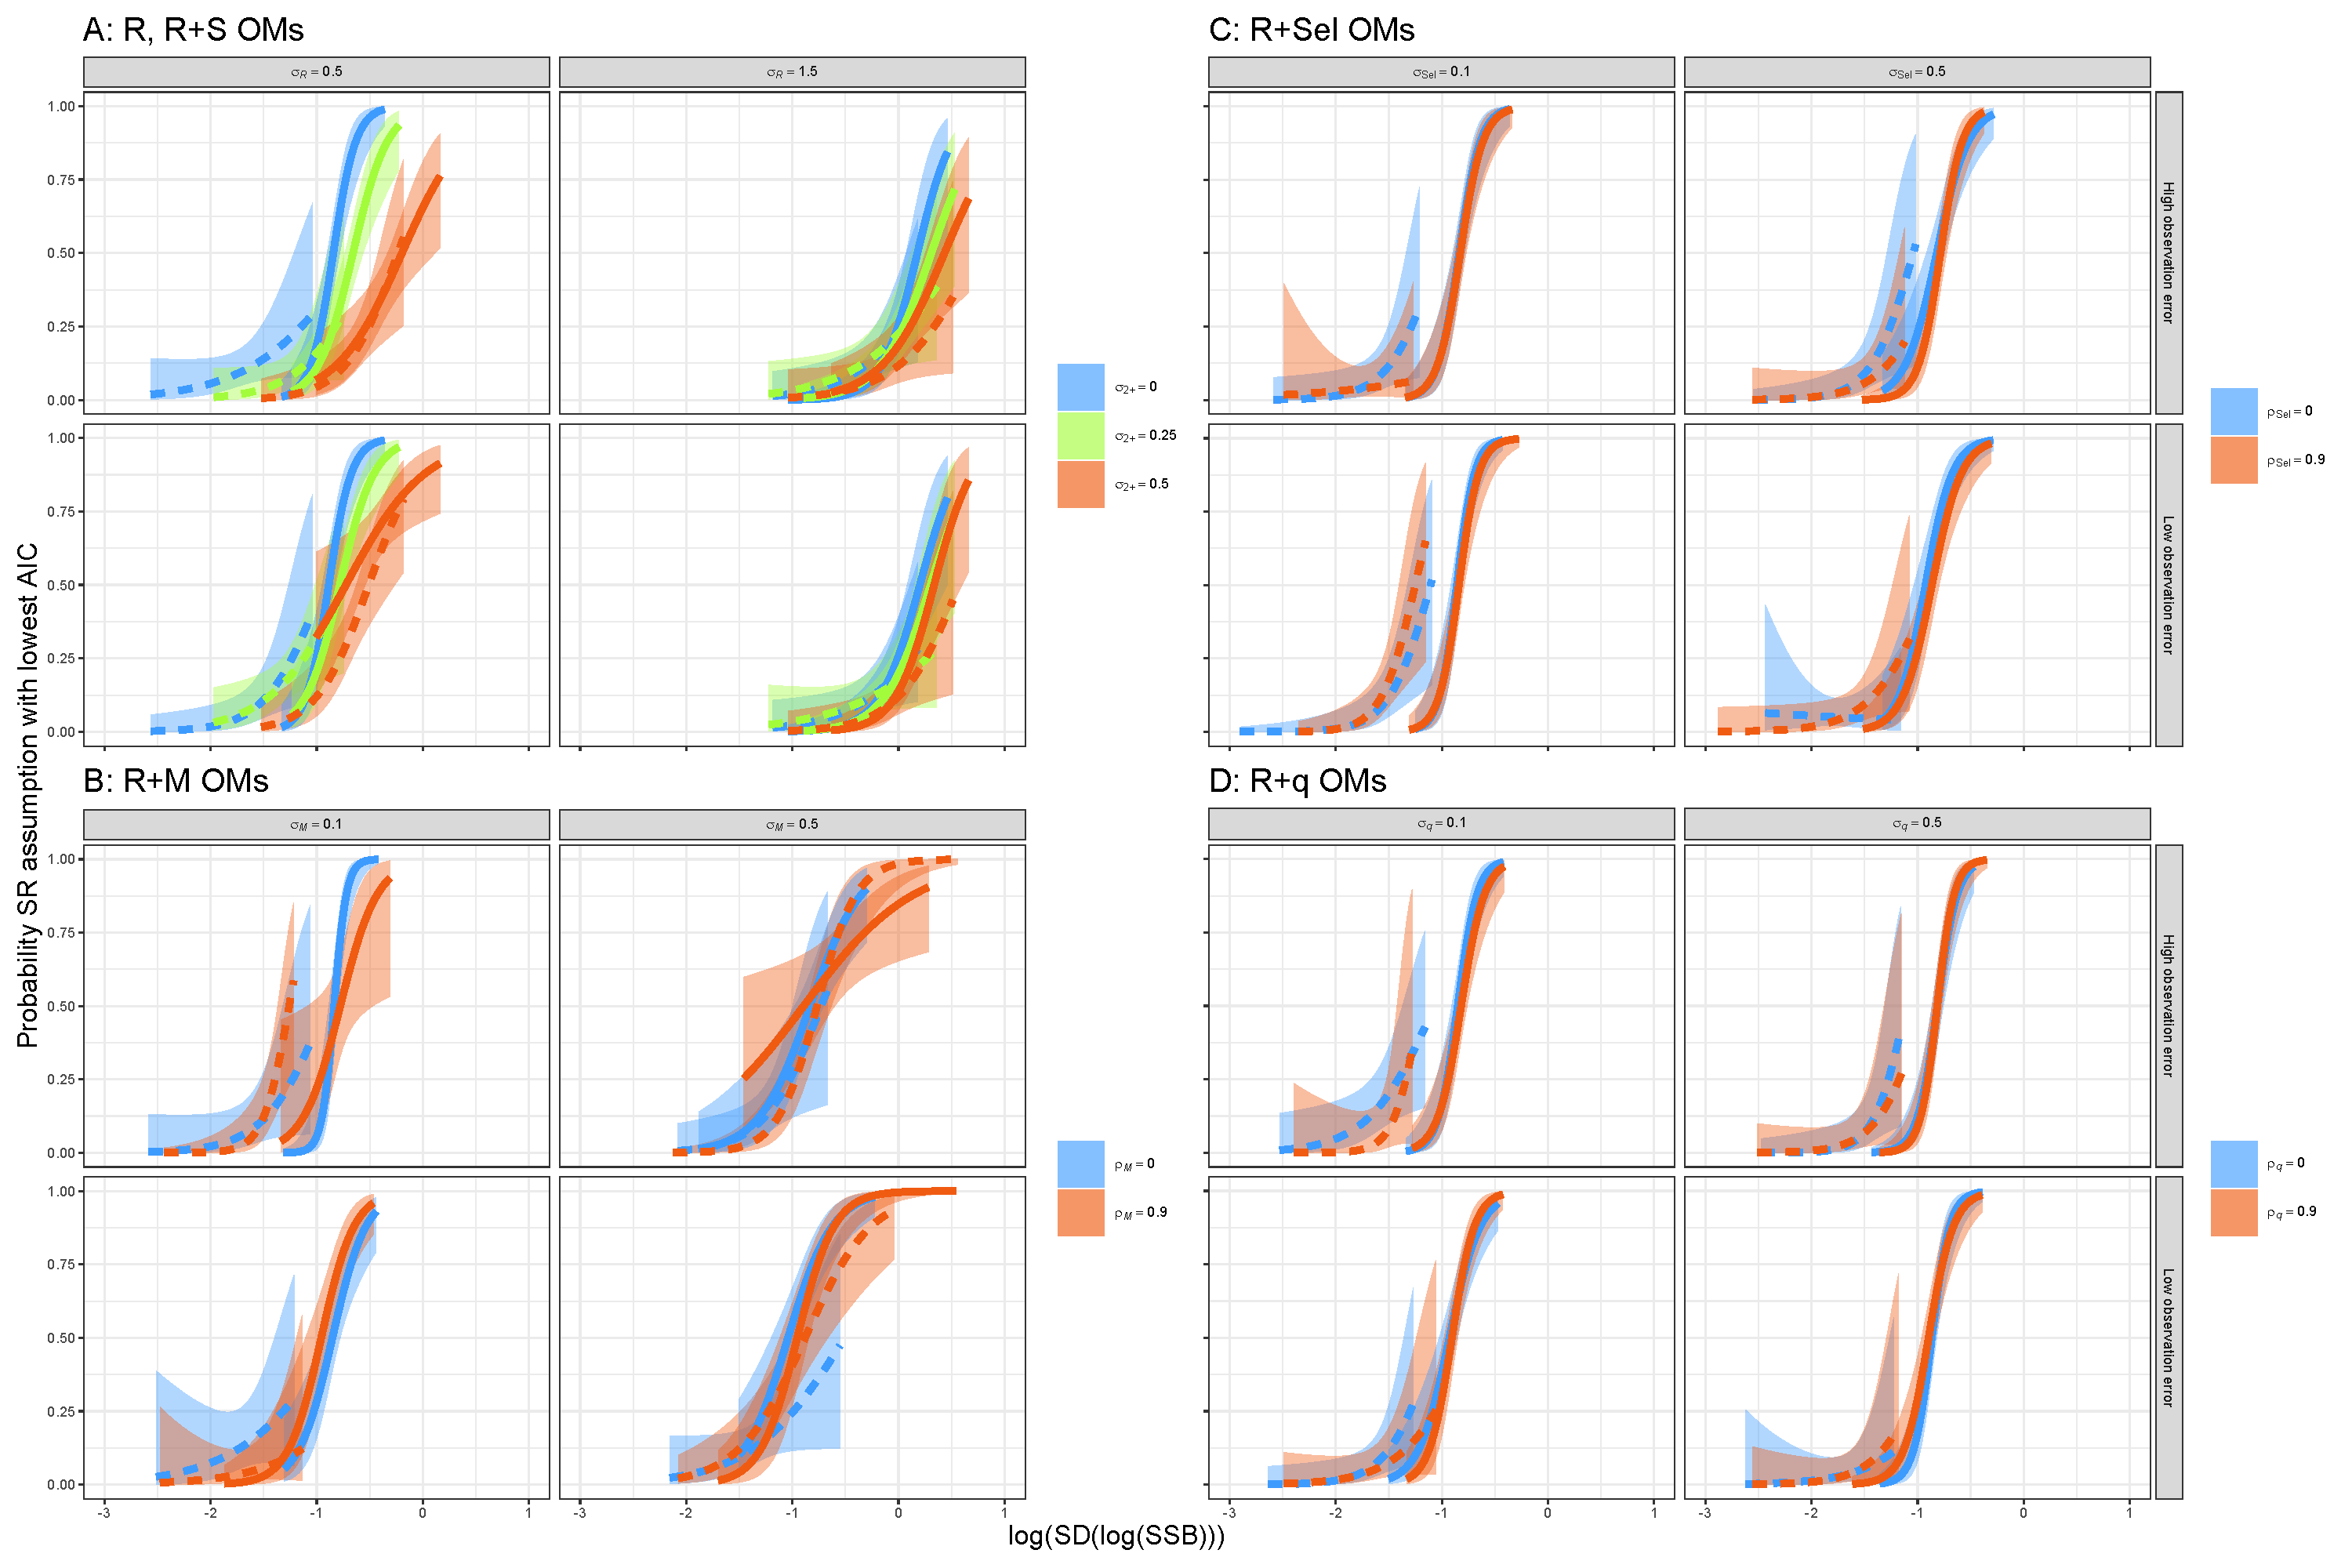
\includegraphics[height = 0.8\textheight]{sr_aic_plots_rev}
\DIFaddendFL \end{center}
\caption{\DIFdelbeginFL \DIFdelFL{Median Mohn's $\rho$ }\DIFdelendFL \DIFaddbeginFL \DIFaddFL{Estimated probability }\DIFaddendFL of \DIFdelbeginFL \DIFdelFL{fishing mortality averaged over all age classes }\DIFdelendFL \DIFaddbeginFL \DIFaddFL{lowest AIC from logistic regression on the log-standard deviation of the true log(SSB) in each simulation }\DIFaddendFL for estimating \DIFdelbeginFL \DIFdelFL{models fitted to data sets simulated }\DIFdelendFL \DIFaddbeginFL \DIFaddFL{model }\DIFaddendFL with \DIFaddbeginFL \DIFaddFL{Beverton-Holt stock-recruit relationships, rather than the otherwise equivalent EM without the stock-recruit relationship. Results are conditional on median M is known in the EM and }\DIFaddendFL alternative \DIFaddbeginFL \DIFaddFL{assumptions EMs having the correct }\DIFaddendFL process error \DIFdelbeginFL \DIFdelFL{structures}\DIFdelendFL \DIFaddbeginFL \DIFaddFL{structure}\DIFaddendFL : R and R+S (A), R+Sel (B), R+M (C), or R+q (D)\DIFdelbeginFL \DIFdelFL{. Circled values indicate results where }\DIFdelendFL \DIFaddbeginFL \DIFaddFL{, and median M is assumed known in }\DIFaddendFL the EM\DIFdelbeginFL \DIFdelFL{process error structure matches that of the operating model }\DIFdelendFL \DIFaddbeginFL \DIFaddFL{. Solid }\DIFaddendFL and \DIFdelbeginFL \DIFdelFL{vertical }\DIFdelendFL \DIFaddbeginFL \DIFaddFL{dashed }\DIFaddendFL lines \DIFaddbeginFL \DIFaddFL{are for OMs with and without temporal contrast in fishing pressure, respectively, and polygons }\DIFaddendFL represent 95\% confidence intervals. \DIFaddbeginFL \DIFaddFL{Range of results indicates the range of log-standard deviation of log(SSB) for simulations of the particular OM.}\DIFaddendFL }\DIFdelbeginFL %DIFDELCMD < \label{mohns_rho_F}
%DIFDELCMD < %%%
\DIFdelendFL \DIFaddbeginFL \label{sr_aic}
\DIFaddendFL \end{figure}
\end{landscape}

\begin{landscape}
\begin{figure}
\begin{center}
\DIFdelbeginFL %DIFDELCMD < 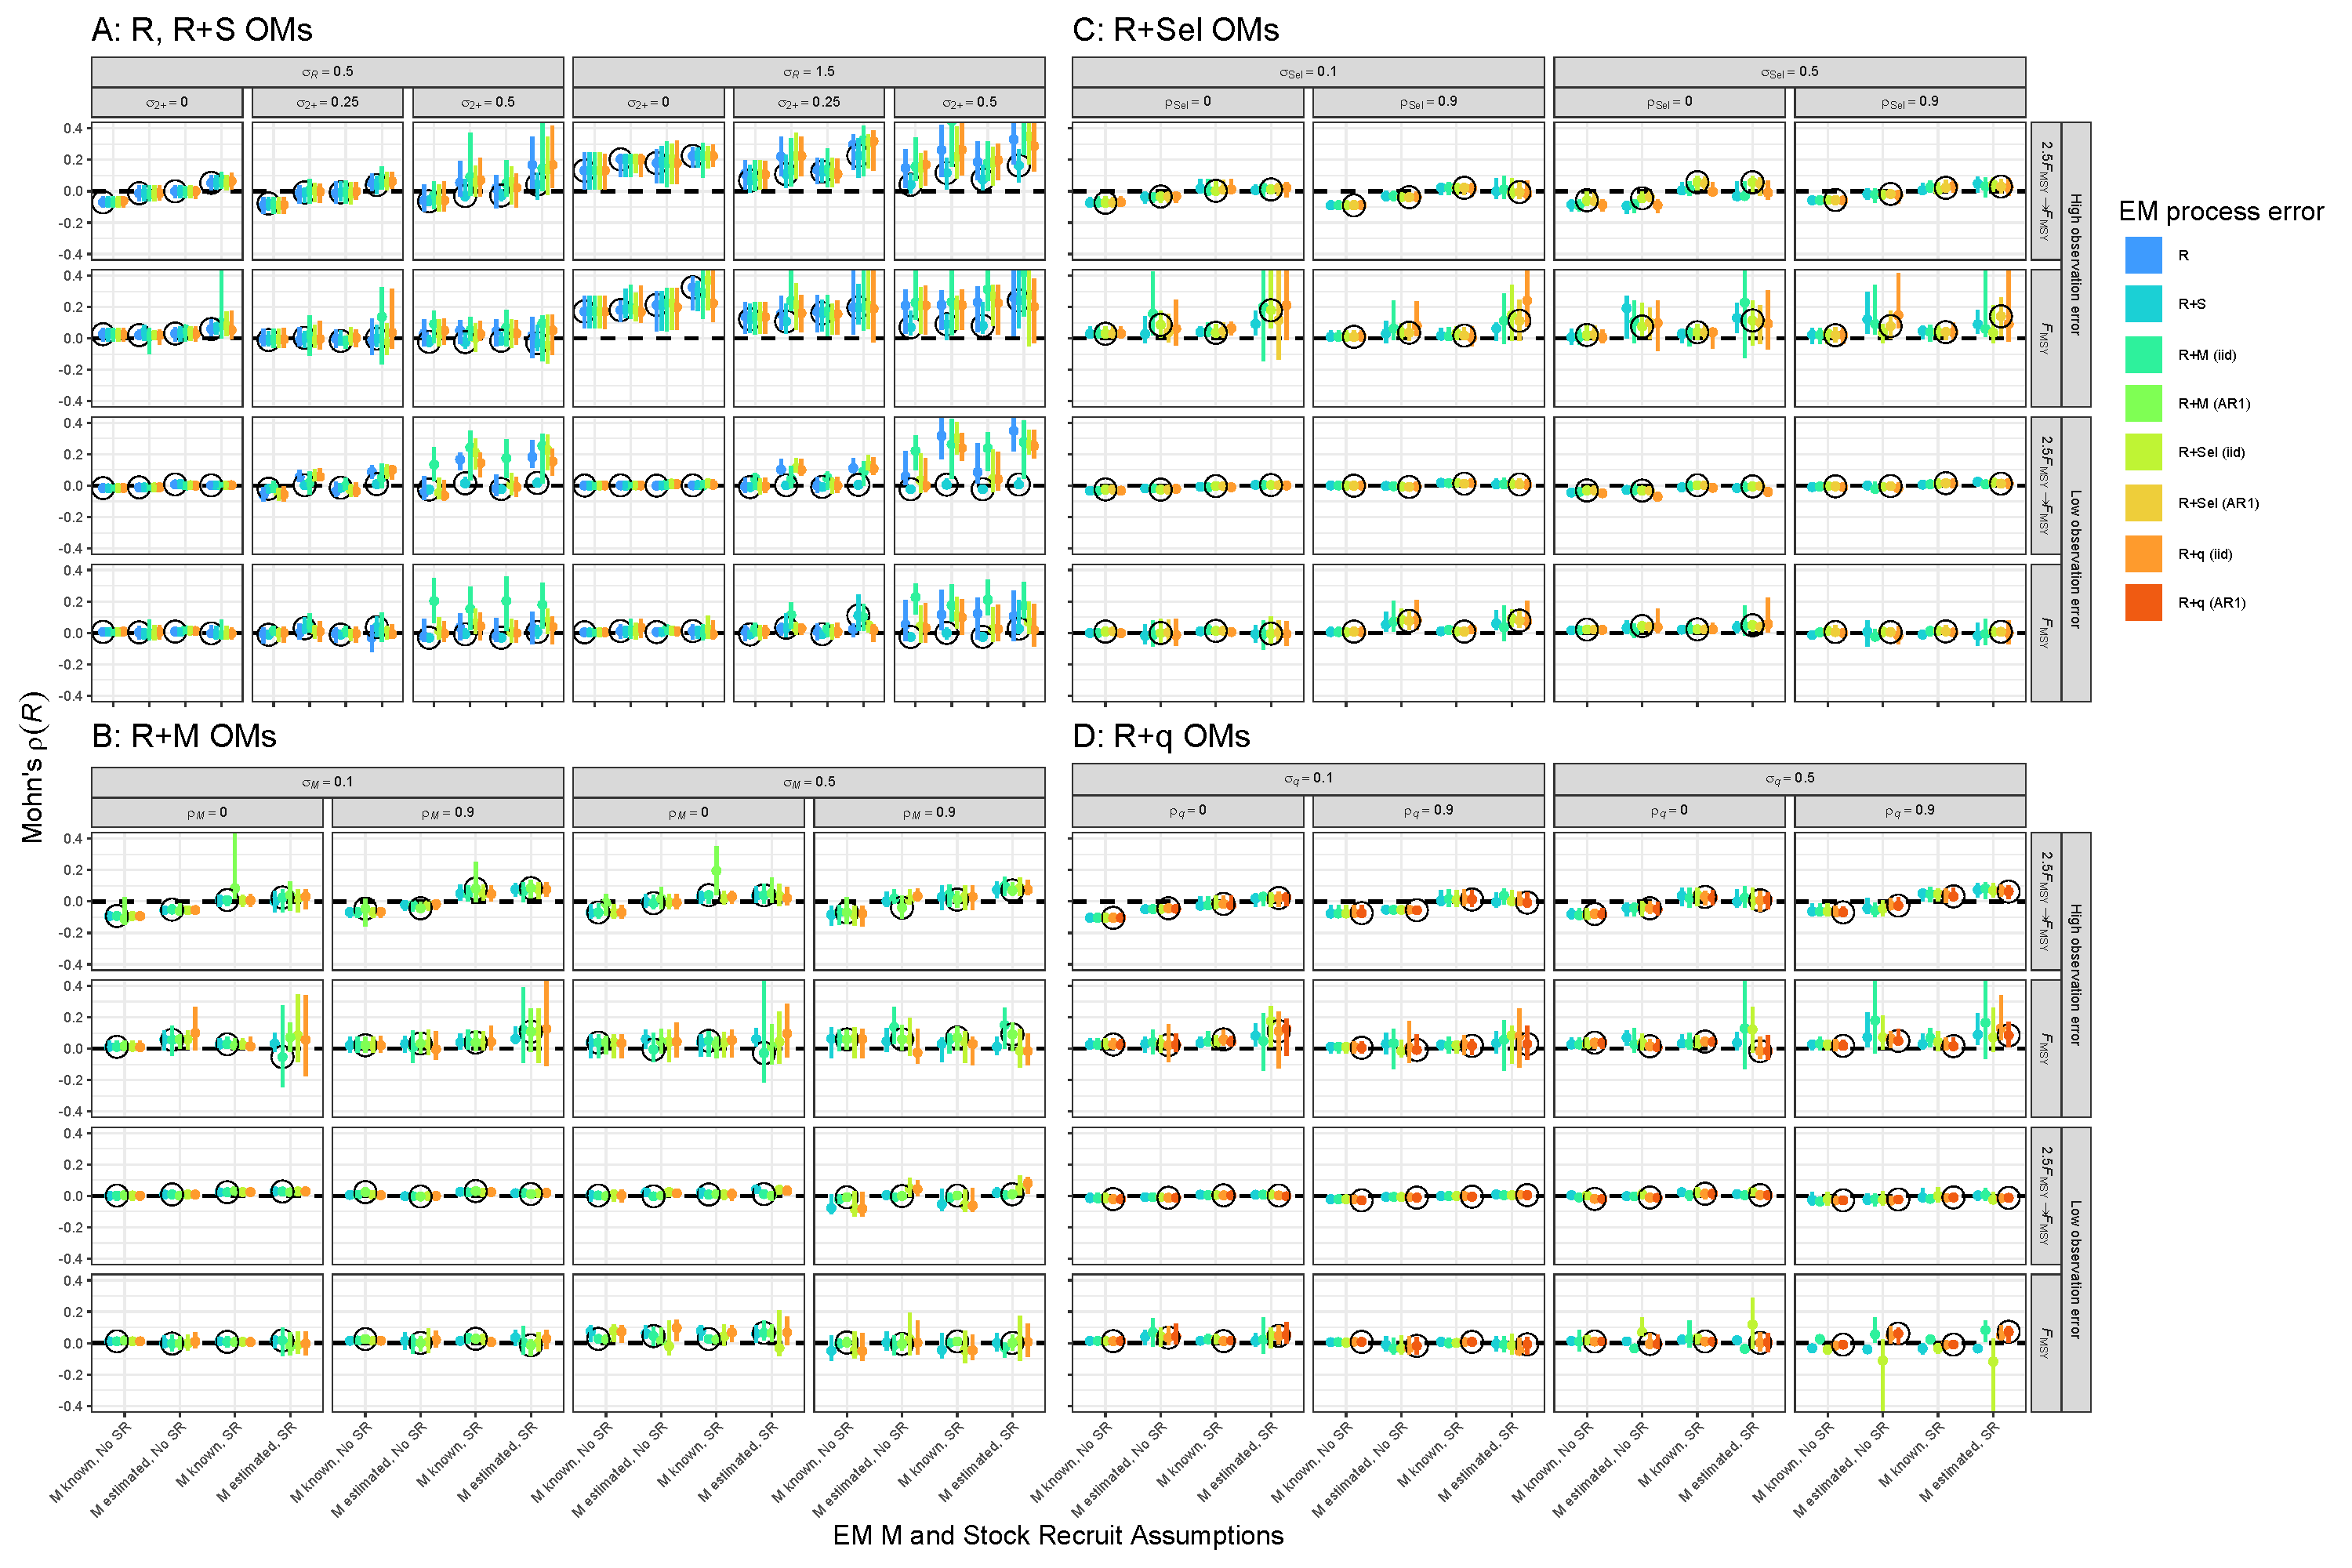
\includegraphics{mohns_rho_R_plots}
%DIFDELCMD < %%%
\DIFdelendFL \DIFaddbeginFL 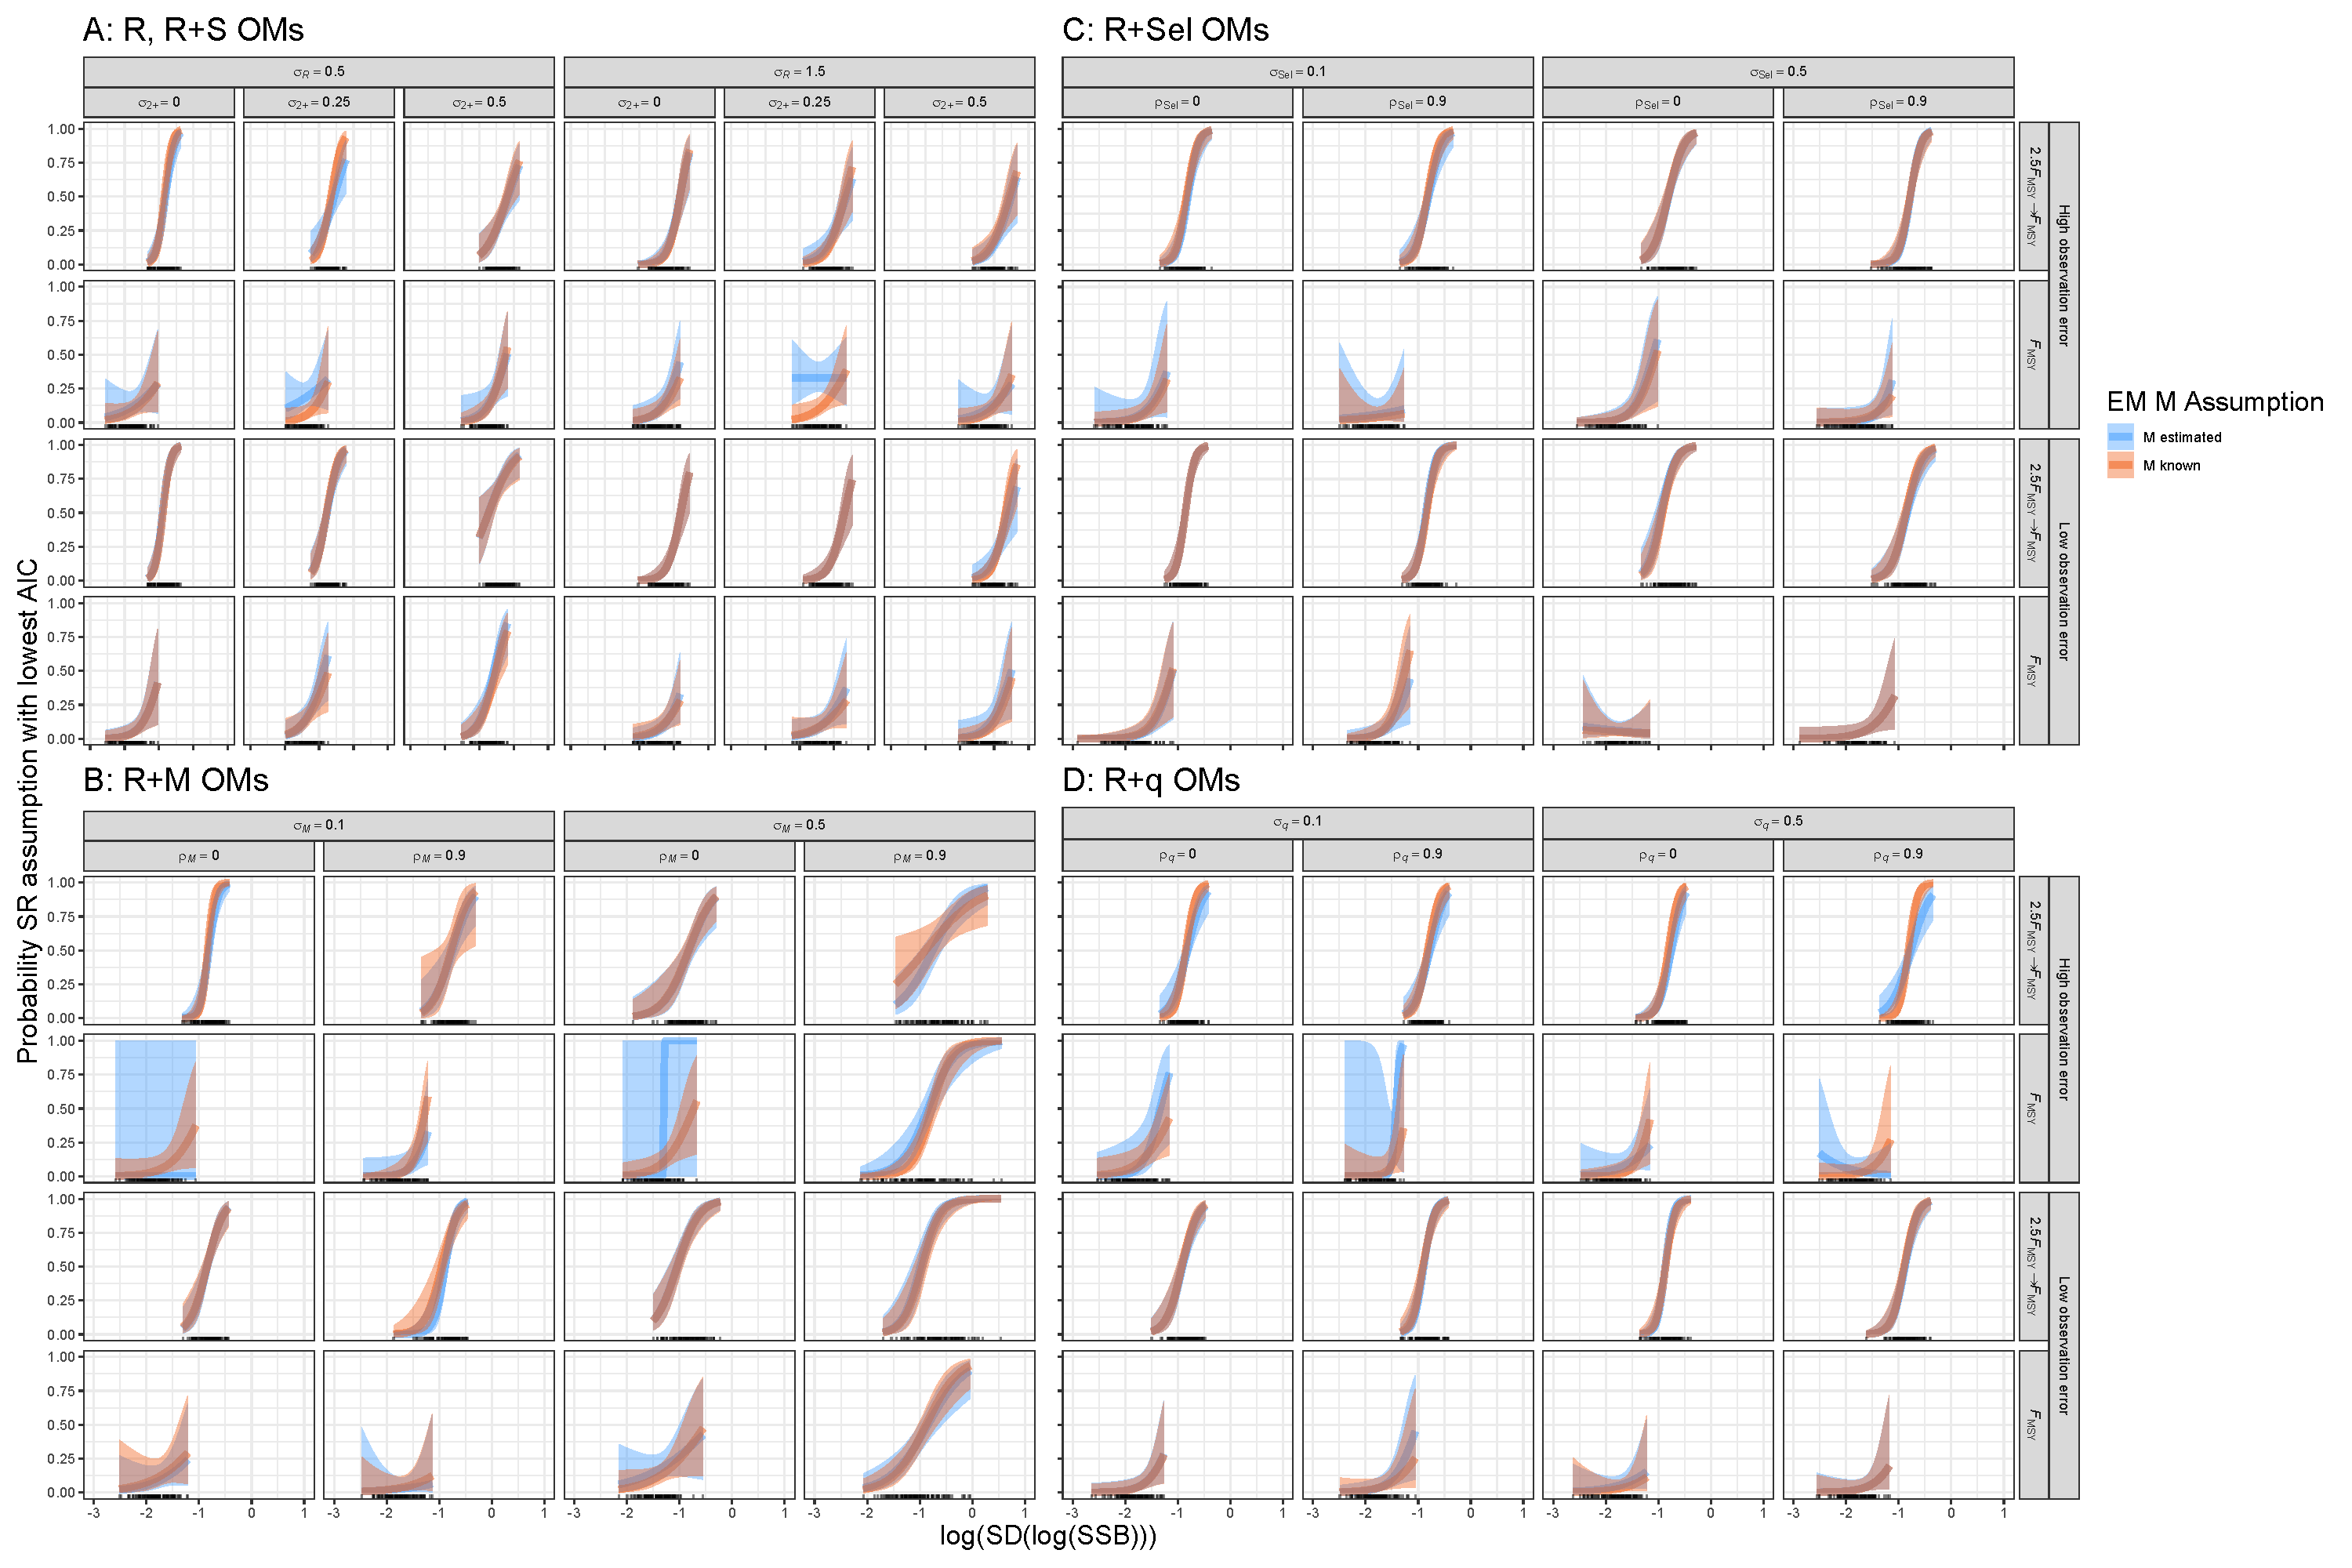
\includegraphics[width = 1.4\textwidth]{sr_aic_plots}
\DIFaddendFL \end{center}
\caption{\DIFdelbeginFL \DIFdelFL{Median Mohn's $\rho$ }\DIFdelendFL \DIFaddbeginFL \DIFaddFL{Estimated probability }\DIFaddendFL of \DIFdelbeginFL \DIFdelFL{recruitment }\DIFdelendFL \DIFaddbeginFL \DIFaddFL{lowest AIC from logistic regression on the log-standard deviation of the true log(SSB) in each simulation }\DIFaddendFL for estimating \DIFdelbeginFL \DIFdelFL{models fitted to data sets simulated }\DIFdelendFL \DIFaddbeginFL \DIFaddFL{model }\DIFaddendFL with \DIFaddbeginFL \DIFaddFL{Beverton-Holt stock-recruit relationships, rather than the otherwise equivalent EM without the stock-recruit relationship. Results are conditional on }\DIFaddendFL alternative \DIFaddbeginFL \DIFaddFL{assumptions for median natural mortality (estimated or known) and on EMs having the correct }\DIFaddendFL process error \DIFdelbeginFL \DIFdelFL{structures}\DIFdelendFL \DIFaddbeginFL \DIFaddFL{structure}\DIFaddendFL : R and R+S (A), R+Sel (B), R+M (C), or R+q (D). \DIFdelbeginFL \DIFdelFL{Circled }\DIFdelendFL \DIFaddbeginFL \DIFaddFL{Rug along x-axis denotes $SD(\log(SSB))$ }\DIFaddendFL values \DIFdelbeginFL \DIFdelFL{indicate results where the EM process error structure matches that of the operating model }\DIFdelendFL \DIFaddbeginFL \DIFaddFL{for each simulation }\DIFaddendFL and \DIFdelbeginFL \DIFdelFL{vertical lines }\DIFdelendFL \DIFaddbeginFL \DIFaddFL{polygons }\DIFaddendFL represent 95\% confidence intervals.}\DIFdelbeginFL %DIFDELCMD < \label{mohns_rho_R}
%DIFDELCMD < %%%
\DIFdelendFL \DIFaddbeginFL \label{sr_aic_supp}
\DIFaddendFL \end{figure}
\end{landscape}
\DIFaddbegin 

\subsubsection*{\DIFadd{Beverton-Holt parameter bias full
results}}\label{beverton-holt-parameter-bias-full-results}
\addcontentsline{toc}{subsubsection}{\DIFadd{Beverton-Holt parameter bias full
results}}

\DIFadd{Across all OMs, there was generally less bias and(or) lower variability
in estimation of the Beverton Holt \(a\) parameter than the \(b\)
parameter. In R and R+S OMs, EMs with the correct assumptions about
process errors provided the least biased estimation of Beverton-Holt SRR
parameters when there was a change in fishing pressure over time and
lower variability of recruitment process errors, but there was little
effect of estimating median natural mortality and a small increase in
bias for those OMs that had high observation error (Figure
\ref{SR_rel_error}, A). For other R and R+S OMs, estimating natural
mortality often resulted in less biased estimation of SRR parameters.
There was generally large variability in relative errors of the SRR
parameter estimates, but the lowest variability occurred with low
variability in recruitment and little or no variability in survival
process errors (\(\sigma_{2+} \in \{0,0.25\}\)), and contrast in fishing
pressure.
}

\DIFadd{In R+M OMs, the most accurate estimation of SRR parameters for all EM
process error assumptions occurred when there was a change in fishing
pressure, greater variability in natural mortality process errors, and
lower observation error (Figure \ref{SR_rel_error}, B). Relative to the
R, and R+S OMs, there was even less effect of estimating median natural
mortality on estimation bias for the SRR parameters.
}

\DIFadd{Bias for SRR parameters was large and variability in relative errors was
greatest for most EMs fit to R+Sel OMs with constant fishing pressure
(Figure \ref{SR_rel_error}, C). Less bias in parameter estimation
occurred for OMs with a change in fishing pressure and the best accuracy
occurred for those OMs that had low observation error and more variable
and uncorrelated selectivity process errors, and when the EMs had with
the correct process error assumption. There was little effect of
estimating natural mortality on relative errors for SRR parameters.
}

\DIFadd{Like R+Sel OMs, relative errors in SRR parameters for R+q OMs were more
accurate for most EM process error types when OMs had contrast in
fishing pressure and lower observation error (Figure \ref{SR_rel_error},
D). However, the best accuracy occurred for those OMs that had lower
variability in catchability process errors. The worst accuracy of SRR
parameter estimation regardless of EM type occurred when R+q OMs had low
observation error and constant fishing pressure (Figure
\ref{SR_rel_error}, D, fourth row).
}

\subsubsection*{\DIFadd{Median natural mortality rate bias full
results}}\label{median-natural-mortality-rate-bias-full-results}
\addcontentsline{toc}{subsubsection}{\DIFadd{Median natural mortality rate bias
full results}}

\DIFadd{Across all OMs and EMs there was little effect of estimating SRRs on the
bias in estimation of median natural mortality (Figure
\ref{M_rel_error}). Median natural mortality rate was estimated
accurately by all EM process error types for all R OMs except those with
high observation error and constant fishing pressure, in which case
relative errors were high (Figure \ref{M_rel_error}, A,
\(\sigma_{2+} = 0\)). For R+S OMs estimation of median natural mortality
rate was most accurate when observation error was low and there was
contrast in fishing pressure and the EM process error type was correct.
}

\DIFadd{For R+M OMs, median natural mortality was estimated most accurately,
regardless of EM process error type, when OMs had a change in fishing
pressure and low observation error (Figure \ref{M_rel_error}, B).
However, those R+M OMs that also had greatest variability in AR1
correlated natural mortality process errors only had unbiased estimation
when the EM process error type was correct.
}

\DIFadd{All EM process error types accurately estimated median natural mortality
rate for R+Sel OMs that had contrast in fishing pressure, low
observation error, and low selectivity process error variability (Figure
\ref{M_rel_error}, C). When selectivity process error variability
increased, the incorrect EM process errors produce more biased
estimation of median natural mortality rate. The least accurate
estimation occurred for all EM process error types when observation
error was high and fishing pressure was constant.
}

\DIFadd{Like R+Sel OMs, all EM process error types produced accurate estimation
of median natural mortality rate when fit to R+q OMs with contrast in
fishing pressure, low observation error and low catchability process
error variability (Figure \ref{M_rel_error}, D). Most EM process error
types produced biased estimation of median natural mortality when R+q
OMs had high observaiton error and constant fishing pressure.
}

\subsubsection*{\DIFadd{Spawning stock biomass bias full
results}}\label{spawning-stock-biomass-bias-full-results}
\addcontentsline{toc}{subsubsection}{\DIFadd{Spawning stock biomass bias full
results}}

\DIFadd{For R OMs (\(\sigma_{2+} = 0\)), there was no indication of bias (95\%
confidence intervals included 0) in terminal year SSB for any of the
estimating models regardless of process error assumptions, except when
no SR assumption was made, recruitment variability was low, and there
was contrast in fishing mortality and high observation error (Figure
\ref{SSB_rel_error}, A). However, errors in terminal SSB estimates were
highly variable when median natural mortality was estimated and there
was constant fishing pressure and high observation error (Figure
\ref{SSB_rel_error}, A, second row).
}

\DIFadd{For R+S OMs, the EMs with matching process error assumptions generally
produced unbiased estimation of terminal SSB except when median natural
mortality was estimated and there was high observation error. In R+S OMs
with low observation error, EMs with incorrect process error assumptions
typically provided biased estimation of terminal year SSB. Estimating
the Beverton-Holt SRR had little discernible effect on bias of terminal
year SSB estimation whereas estimating median M tended to produce more
variability in errors in terminal SSB estimation similar to R OMs.
}

\DIFadd{For R+ M OMs with low variability in natural mortality process errors,
low observation error and contrast in fishing motality over time all EMs
produced low variability in SSB estimation error that indicated
unbiasedness (Figure \ref{SSB_rel_error}, B, third row). However, larger
variability in natural mortality process errors increased bias of EMs
without the correct process error type. Estimating median natural
mortality increased variability of SSB estimation error particularly for
OMs with high observation error and constant fishing pressure over time.
It also increased bias in SSB estimation for many R+M OMs. Like R and
R+S OMs, estimating a SRR had little discernible effect on SSB bias.
}

\DIFadd{For R+Sel OMs, there was no evidence of bias for any EMs when
variability in selectivity process error and observation error was low,
and with contrast in fishing mortality (Figure \ref{SSB_rel_error}, C).
The largest bias occurred for any EMs that estimated median natural
mortality when the OMs had high observation error, constant fishing
pressure, and greater variability in selectivity process errors
(\(\sigma_{\text{Sel}} = 0.5\)) or low selectivity process errors
(\(\sigma_{\text{Sel}} = 0.1\)) and low observation error. However,
there was no evidence of SSB bias for correctly specified R+Sel EMs when
observation error was low and variation in selectivity process errors
was larger, whether median natural mortality was estimated or not
(Figure \ref{SSB_rel_error}, C, third row). We only observed an effect
of estimating the Beverton-Holt SRR for R+Sel OMs that had high
observation error and contrast in fishing pressure where estimating the
SRR produced less biased SSB estimation for many EMs (Figure
\ref{SSB_rel_error}, C, top row).
}

\DIFadd{All EMs fit to data from R+q OMs with low observation error and contrast
in fishing pressure exhibited little evidence of bias in terminal SSB
estimation except for R+M EMs when there was no AR1 correlation in
catchability process errors (Figure \ref{SSB_rel_error}, D). Many EMs
also performed well in R+q OMs with low observation error, but no
contrast in fishing pressure. For R+q OMs with high observation error
and contrast in fishing pressure, EMs that estimated the Beverton-Holt
SRR exhibited less SSB bias than those that did not. Estimating median
natural mortality in the EMs only resulted in much more variable SSB
estimation errors when there was no contrast in fishing pressure (Figure
\ref{SSB_rel_error}, D, first and third rows).
}

\DIFadd{For all OM process error types, relative errors in terminal year
recruitment were generally more variable than SSB, but effects of R and
R+S OM and EM attributes on bias (i.e, negative or positive or none)
were similar (Figure \ref{R_rel_error}, A). Furthermore, for EM
configurations where bias in terminal SSB was evident, median relative
errors in recruitment often indicated stronger bias in recruitment of
the same sign.
}

\subsubsection*{\texorpdfstring{Mohn's \(\rho\) Full
results}{Mohn's \textbackslash rho Full results}}\label{mohns-rho-full-results}
\addcontentsline{toc}{subsubsection}{\DIFadd{Mohn's \(\rho\) Full results}}

\DIFadd{Mohn's \(\rho\) for SSB was small in absolute value for all R and R+S
OMs, regardless of EM process error types, and whether median natural
mortality rate or SRRs were estimated (Figure \ref{mohns_rho_ssb}, A).
The strongest retrospective patterns (highest absolute Mohn's \(\rho\)
values) occurred in OMs with the largest apparent survival process error
variability, high observation error, and contrast in fishing pressure,
but only for EMs with the incorrect process error type and where median
natural mortality rate was assumed known (median \(\rho\) was
approximately -0.15). For R+M, R+Sel, and R+q OMs, Mohn's \(\rho\) was
also small in absolute value, but median values were all closer to 0
than the largest values in the R and R+S OMs (Figure
\ref{mohns_rho_ssb},B-D). For these OMs, there was no noticeable effect
of estimation of median natural mortality rate or SRRs on Mohn's
\(\rho\) for any EM process error types.
}

\DIFadd{Mohn's \(\rho\) for recruitment was small in absolute value for all R
OMs with low variability in recruitment process errors, regardless of EM
process error type, and whether median natural mortality rate or SRRs
were estimated (Figure \ref{mohns_rho_R}, A). However, R and R+S OMs
with greater recruitment process variability and higher observation
error had median Mohn's \(\rho\) for recruitment greater than zero for
most EMs even when the EM process error type was correct. In R+S OMs
with lower observation error, EMs with the correct process error type
exhibited better median Mohn's \(\rho\) close to 0 than EMs with the
incorrect process error type. For R+M, R+Sel, and R+q OMs, results for
Mohn's \(\rho\) for recruitment are similar to those for SSB, but the
range in median values and variation in Mohn's \(\rho\) values for a
given OM are generally larger for recruitment (Figure \ref{mohns_rho_R},
B-D).
}\DIFaddend 

\end{document}
